\documentclass{book}
\usepackage[a4paper,top=2.5cm,bottom=2.5cm,left=2.5cm,right=2.5cm]{geometry}
\usepackage{makeidx}
\usepackage{natbib}
\usepackage{graphicx}
\usepackage{multicol}
\usepackage{float}
\usepackage{listings}
\usepackage{color}
\usepackage{ifthen}
\usepackage[table]{xcolor}
\usepackage{textcomp}
\usepackage{alltt}
\usepackage{ifpdf}
\ifpdf
\usepackage[pdftex,
            pagebackref=true,
            colorlinks=true,
            linkcolor=blue,
            unicode
           ]{hyperref}
\else
\usepackage[ps2pdf,
            pagebackref=true,
            colorlinks=true,
            linkcolor=blue,
            unicode
           ]{hyperref}
\usepackage{pspicture}
\fi
\usepackage[utf8]{inputenc}
\usepackage{mathptmx}
\usepackage[scaled=.90]{helvet}
\usepackage{courier}
\usepackage{sectsty}
\usepackage{amssymb}
\usepackage[titles]{tocloft}
\usepackage{doxygen}
\lstset{language=C++,inputencoding=utf8,basicstyle=\footnotesize,breaklines=true,breakatwhitespace=true,tabsize=4,numbers=left }
\makeindex
\setcounter{tocdepth}{3}
\renewcommand{\footrulewidth}{0.4pt}
\renewcommand{\familydefault}{\sfdefault}
\hfuzz=15pt
\setlength{\emergencystretch}{15pt}
\hbadness=750
\tolerance=750
\begin{document}
\hypersetup{pageanchor=false,citecolor=blue}
\begin{titlepage}
\vspace*{7cm}
\begin{center}
{\Large Software\-\_\-\-Engineering\-A6 }\\
\vspace*{1cm}
{\large Generated by Doxygen 1.8.3.1}\\
\vspace*{0.5cm}
{\small Thu May 2 2013 14:49:23}\\
\end{center}
\end{titlepage}
\clearemptydoublepage
\pagenumbering{roman}
\tableofcontents
\clearemptydoublepage
\pagenumbering{arabic}
\hypersetup{pageanchor=true,citecolor=blue}
\chapter{Hierarchical Index}
\section{Class Hierarchy}
This inheritance list is sorted roughly, but not completely, alphabetically\-:\begin{DoxyCompactList}
\item Abstract\-Color\-Chooser\-Panel\begin{DoxyCompactList}
\item \contentsline{section}{Colour}{\pageref{class_colour}}{}
\end{DoxyCompactList}
\item \contentsline{section}{Chart}{\pageref{interface_chart}}{}
\begin{DoxyCompactList}
\item \contentsline{section}{Pie\-Chart}{\pageref{class_pie_chart}}{}
\end{DoxyCompactList}
\item \contentsline{section}{Data\-Attribute}{\pageref{class_data_attribute}}{}
\item \contentsline{section}{Dataset}{\pageref{class_dataset}}{}
\item \contentsline{section}{Error}{\pageref{class_error}}{}
\item \contentsline{section}{Graph}{\pageref{interface_graph}}{}
\begin{DoxyCompactList}
\item \contentsline{section}{Area\-Chart}{\pageref{class_area_chart}}{}
\item \contentsline{section}{Bubble\-Chart}{\pageref{class_bubble_chart}}{}
\item \contentsline{section}{Line\-Chart}{\pageref{class_line_chart}}{}
\item \contentsline{section}{Polar\-Chart}{\pageref{class_polar_chart}}{}
\item \contentsline{section}{Scatter\-Plot\-Graph}{\pageref{class_scatter_plot_graph}}{}
\end{DoxyCompactList}
\item \contentsline{section}{Group\-P\-D\-M2application}{\pageref{class_group_p_d_m2application}}{}
\item Action\-Listener\begin{DoxyCompactList}
\item \contentsline{section}{Area\-Chart}{\pageref{class_area_chart}}{}
\item \contentsline{section}{Bubble\-Chart}{\pageref{class_bubble_chart}}{}
\item \contentsline{section}{Colour}{\pageref{class_colour}}{}
\item \contentsline{section}{Colour\-Map}{\pageref{class_colour_map}}{}
\item \contentsline{section}{Column\-Chart}{\pageref{class_column_chart}}{}
\item \contentsline{section}{Line\-Chart}{\pageref{class_line_chart}}{}
\item \contentsline{section}{Pie\-Chart}{\pageref{class_pie_chart}}{}
\item \contentsline{section}{Polar\-Chart}{\pageref{class_polar_chart}}{}
\item \contentsline{section}{Scatter\-Plot\-Graph}{\pageref{class_scatter_plot_graph}}{}
\end{DoxyCompactList}
\item Change\-Listener\begin{DoxyCompactList}
\item \contentsline{section}{Colour\-Map}{\pageref{class_colour_map}}{}
\end{DoxyCompactList}
\item J\-Frame\begin{DoxyCompactList}
\item \contentsline{section}{Bob\-Viz}{\pageref{class_bob_viz}}{}
\item \contentsline{section}{More\-Setting\-J\-Panel}{\pageref{class_more_setting_j_panel}}{}
\item \contentsline{section}{Pie\-Chart}{\pageref{class_pie_chart}}{}
\item \contentsline{section}{Slideshow}{\pageref{class_slideshow}}{}
\end{DoxyCompactList}
\item J\-Panel\begin{DoxyCompactList}
\item \contentsline{section}{About\-J\-Panel}{\pageref{class_about_j_panel}}{}
\item \contentsline{section}{Colour\-Map}{\pageref{class_colour_map}}{}
\item \contentsline{section}{Import\-J\-Panel}{\pageref{class_import_j_panel}}{}
\item \contentsline{section}{Information\-J\-Panel}{\pageref{class_information_j_panel}}{}
\item \contentsline{section}{Selection\-Viz\-J\-Panel}{\pageref{class_selection_viz_j_panel}}{}
\item \contentsline{section}{Setting\-J\-Panel}{\pageref{class_setting_j_panel}}{}
\item \contentsline{section}{Status\-J\-Panel}{\pageref{class_status_j_panel}}{}
\item \contentsline{section}{Table}{\pageref{class_table}}{}
\item \contentsline{section}{Visualisation}{\pageref{class_visualisation}}{}
\item \contentsline{section}{Viz\-Type\-J\-Panel}{\pageref{class_viz_type_j_panel}}{}
\end{DoxyCompactList}
\end{DoxyCompactList}

\chapter{Class Index}
\section{Class List}
Here are the classes, structs, unions and interfaces with brief descriptions\-:\begin{DoxyCompactList}
\item\contentsline{section}{\hyperlink{class_about_j_panel}{About\-J\-Panel} \\*This class provides the user with information about the application }{\pageref{class_about_j_panel}}{}
\item\contentsline{section}{\hyperlink{class_area_chart}{Area\-Chart} \\*A class that creates a single Area \hyperlink{interface_chart}{Chart} or two Area Charts visualizations from a 2\-D Array of data \textbackslash{} see \hyperlink{_graph_8java}{Graph.\-java} }{\pageref{class_area_chart}}{}
\item\contentsline{section}{\hyperlink{class_bob_viz}{Bob\-Viz} \\*This class provides the user with a simple G\-U\-I system. It initiates all instances used throughout the application }{\pageref{class_bob_viz}}{}
\item\contentsline{section}{\hyperlink{class_bubble_chart}{Bubble\-Chart} \\*A class that creates a single Bubble \hyperlink{interface_chart}{Chart} or two Bubble \hyperlink{interface_chart}{Chart} visualizations from a 2\-D Array of data \textbackslash{} see \hyperlink{_graph_8java}{Graph.\-java} }{\pageref{class_bubble_chart}}{}
\item\contentsline{section}{\hyperlink{interface_chart}{Chart} \\*An interface for all chart classes }{\pageref{interface_chart}}{}
\item\contentsline{section}{\hyperlink{class_colour}{Colour} \\*This class provides user with a choice of some colours to be applied on objects from different graphs/charts/diagrams }{\pageref{class_colour}}{}
\item\contentsline{section}{\hyperlink{class_colour_map}{Colour\-Map} \\*This class provides user with a choice of colours to be applied on objects from different graphs/charts/diagrams, and does all calculations needed in order to get it all working correctly }{\pageref{class_colour_map}}{}
\item\contentsline{section}{\hyperlink{class_column_chart}{Column\-Chart} \\*A class that displays specific data in a Column \hyperlink{interface_chart}{Chart} visualiser }{\pageref{class_column_chart}}{}
\item\contentsline{section}{\hyperlink{class_data_attribute}{Data\-Attribute} \\*A class which is responsible setting graph attributes }{\pageref{class_data_attribute}}{}
\item\contentsline{section}{\hyperlink{class_dataset}{Dataset} \\*A Class that Reads a data file format 'C\-S\-V' and Creates a 2\-D array and has methods to extract columns of data }{\pageref{class_dataset}}{}
\item\contentsline{section}{\hyperlink{class_error}{Error} \\*A class designed to deal with errors and alerts the user }{\pageref{class_error}}{}
\item\contentsline{section}{\hyperlink{interface_graph}{Graph} \\*An interface for all graph classes }{\pageref{interface_graph}}{}
\item\contentsline{section}{\hyperlink{class_group_p_d_m2application}{Group\-P\-D\-M2application} \\*This class creates a new instance of \hyperlink{class_bob_viz}{Bob\-Viz} and parses it to all panels to ensure only one instance of \hyperlink{class_bob_viz}{Bob\-Viz} is ever used }{\pageref{class_group_p_d_m2application}}{}
\item\contentsline{section}{\hyperlink{class_import_j_panel}{Import\-J\-Panel} \\*This class provides a import (C\-S\-V file) procedure }{\pageref{class_import_j_panel}}{}
\item\contentsline{section}{\hyperlink{class_information_j_panel}{Information\-J\-Panel} \\*A class designed to deal with the Information panel }{\pageref{class_information_j_panel}}{}
\item\contentsline{section}{\hyperlink{class_line_chart}{Line\-Chart} \\*A class that creates a Line \hyperlink{interface_chart}{Chart} visualisation from a 2\-D Array of data }{\pageref{class_line_chart}}{}
\item\contentsline{section}{\hyperlink{class_more_setting_j_panel}{More\-Setting\-J\-Panel} \\*A class designed to deal with the 'More Settings' panel }{\pageref{class_more_setting_j_panel}}{}
\item\contentsline{section}{\hyperlink{class_pie_chart}{Pie\-Chart} \\*A simple class that displays data in a single Pie \hyperlink{interface_chart}{Chart}, or two Pie \hyperlink{interface_chart}{Chart} visualisations }{\pageref{class_pie_chart}}{}
\item\contentsline{section}{\hyperlink{class_polar_chart}{Polar\-Chart} \\*A class that creates a single Polar \hyperlink{interface_chart}{Chart} or two Polar \hyperlink{interface_chart}{Chart} visualisations from 2\-D Arrays of data \textbackslash{} see \hyperlink{_graph_8java}{Graph.\-java} }{\pageref{class_polar_chart}}{}
\item\contentsline{section}{\hyperlink{class_scatter_plot_graph}{Scatter\-Plot\-Graph} \\*A class that creates a single Scatter Plot \hyperlink{interface_graph}{Graph} or two Scatter Plot \hyperlink{interface_graph}{Graph} visualisations from a 2\-D Array of data }{\pageref{class_scatter_plot_graph}}{}
\item\contentsline{section}{\hyperlink{class_selection_viz_j_panel}{Selection\-Viz\-J\-Panel} \\*This class passes the data from the G\-U\-I to the constructors of the visualisation types }{\pageref{class_selection_viz_j_panel}}{}
\item\contentsline{section}{\hyperlink{class_setting_j_panel}{Setting\-J\-Panel} \\*This class provides the settings for each visualisation }{\pageref{class_setting_j_panel}}{}
\item\contentsline{section}{\hyperlink{class_slideshow}{Slideshow} \\*A class that creates a slideshow of a single \hyperlink{interface_chart}{Chart} or two \hyperlink{interface_chart}{Chart} visualizations \textbackslash{} see \hyperlink{_graph_8java}{Graph.\-java} }{\pageref{class_slideshow}}{}
\item\contentsline{section}{\hyperlink{class_status_j_panel}{Status\-J\-Panel} \\*This class will display the status of the application }{\pageref{class_status_j_panel}}{}
\item\contentsline{section}{\hyperlink{class_table}{Table} \\*A simple class that displays data in a table visualisation }{\pageref{class_table}}{}
\item\contentsline{section}{\hyperlink{class_visualisation}{Visualisation} \\*A class that displays specific data in a Column \hyperlink{interface_chart}{Chart} visualiser }{\pageref{class_visualisation}}{}
\item\contentsline{section}{\hyperlink{class_viz_type_j_panel}{Viz\-Type\-J\-Panel} \\*This class provides the user with a list of different visualisation types to choose from }{\pageref{class_viz_type_j_panel}}{}
\end{DoxyCompactList}

\chapter{File Index}
\section{File List}
Here is a list of all files with brief descriptions\-:\begin{DoxyCompactList}
\item\contentsline{section}{\hyperlink{_about_j_panel_8java}{About\-J\-Panel.\-java} }{\pageref{_about_j_panel_8java}}{}
\item\contentsline{section}{\hyperlink{_area_chart_8java}{Area\-Chart.\-java} }{\pageref{_area_chart_8java}}{}
\item\contentsline{section}{\hyperlink{_bob_viz_8java}{Bob\-Viz.\-java} }{\pageref{_bob_viz_8java}}{}
\item\contentsline{section}{\hyperlink{_bubble_chart_8java}{Bubble\-Chart.\-java} }{\pageref{_bubble_chart_8java}}{}
\item\contentsline{section}{\hyperlink{_chart_8java}{Chart.\-java} }{\pageref{_chart_8java}}{}
\item\contentsline{section}{\hyperlink{_colour_8java}{Colour.\-java} }{\pageref{_colour_8java}}{}
\item\contentsline{section}{\hyperlink{_colour_map_8java}{Colour\-Map.\-java} }{\pageref{_colour_map_8java}}{}
\item\contentsline{section}{\hyperlink{_column_chart_8java}{Column\-Chart.\-java} }{\pageref{_column_chart_8java}}{}
\item\contentsline{section}{\hyperlink{_data_attribute_8java}{Data\-Attribute.\-java} }{\pageref{_data_attribute_8java}}{}
\item\contentsline{section}{\hyperlink{_dataset_8java}{Dataset.\-java} }{\pageref{_dataset_8java}}{}
\item\contentsline{section}{\hyperlink{_error_8java}{Error.\-java} }{\pageref{_error_8java}}{}
\item\contentsline{section}{\hyperlink{_graph_8java}{Graph.\-java} }{\pageref{_graph_8java}}{}
\item\contentsline{section}{\hyperlink{_group_p_d_m2application_8java}{Group\-P\-D\-M2application.\-java} }{\pageref{_group_p_d_m2application_8java}}{}
\item\contentsline{section}{\hyperlink{_import_j_panel_8java}{Import\-J\-Panel.\-java} }{\pageref{_import_j_panel_8java}}{}
\item\contentsline{section}{\hyperlink{_information_j_panel_8java}{Information\-J\-Panel.\-java} }{\pageref{_information_j_panel_8java}}{}
\item\contentsline{section}{\hyperlink{_line_chart_8java}{Line\-Chart.\-java} }{\pageref{_line_chart_8java}}{}
\item\contentsline{section}{\hyperlink{_more_setting_j_panel_8java}{More\-Setting\-J\-Panel.\-java} }{\pageref{_more_setting_j_panel_8java}}{}
\item\contentsline{section}{\hyperlink{_pie_chart_8java}{Pie\-Chart.\-java} }{\pageref{_pie_chart_8java}}{}
\item\contentsline{section}{\hyperlink{_polar_chart_8java}{Polar\-Chart.\-java} }{\pageref{_polar_chart_8java}}{}
\item\contentsline{section}{\hyperlink{_scatter_plot_graph_8java}{Scatter\-Plot\-Graph.\-java} }{\pageref{_scatter_plot_graph_8java}}{}
\item\contentsline{section}{\hyperlink{_selection_viz_j_panel_8java}{Selection\-Viz\-J\-Panel.\-java} }{\pageref{_selection_viz_j_panel_8java}}{}
\item\contentsline{section}{\hyperlink{_setting_j_panel_8java}{Setting\-J\-Panel.\-java} }{\pageref{_setting_j_panel_8java}}{}
\item\contentsline{section}{\hyperlink{_slideshow_8java}{Slideshow.\-java} }{\pageref{_slideshow_8java}}{}
\item\contentsline{section}{\hyperlink{_status_j_panel_8java}{Status\-J\-Panel.\-java} }{\pageref{_status_j_panel_8java}}{}
\item\contentsline{section}{\hyperlink{_table_8java}{Table.\-java} }{\pageref{_table_8java}}{}
\item\contentsline{section}{\hyperlink{_time_stamp_8java}{Time\-Stamp.\-java} }{\pageref{_time_stamp_8java}}{}
\item\contentsline{section}{\hyperlink{_visualisation_8java}{Visualisation.\-java} }{\pageref{_visualisation_8java}}{}
\item\contentsline{section}{\hyperlink{_viz_type_j_panel_8java}{Viz\-Type\-J\-Panel.\-java} }{\pageref{_viz_type_j_panel_8java}}{}
\end{DoxyCompactList}

\chapter{Class Documentation}
\hypertarget{class_about_j_panel}{\section{About\-J\-Panel Class Reference}
\label{class_about_j_panel}\index{About\-J\-Panel@{About\-J\-Panel}}
}


This class provides the user with information about the application.  


Inheritance diagram for About\-J\-Panel\-:\begin{figure}[H]
\begin{center}
\leavevmode
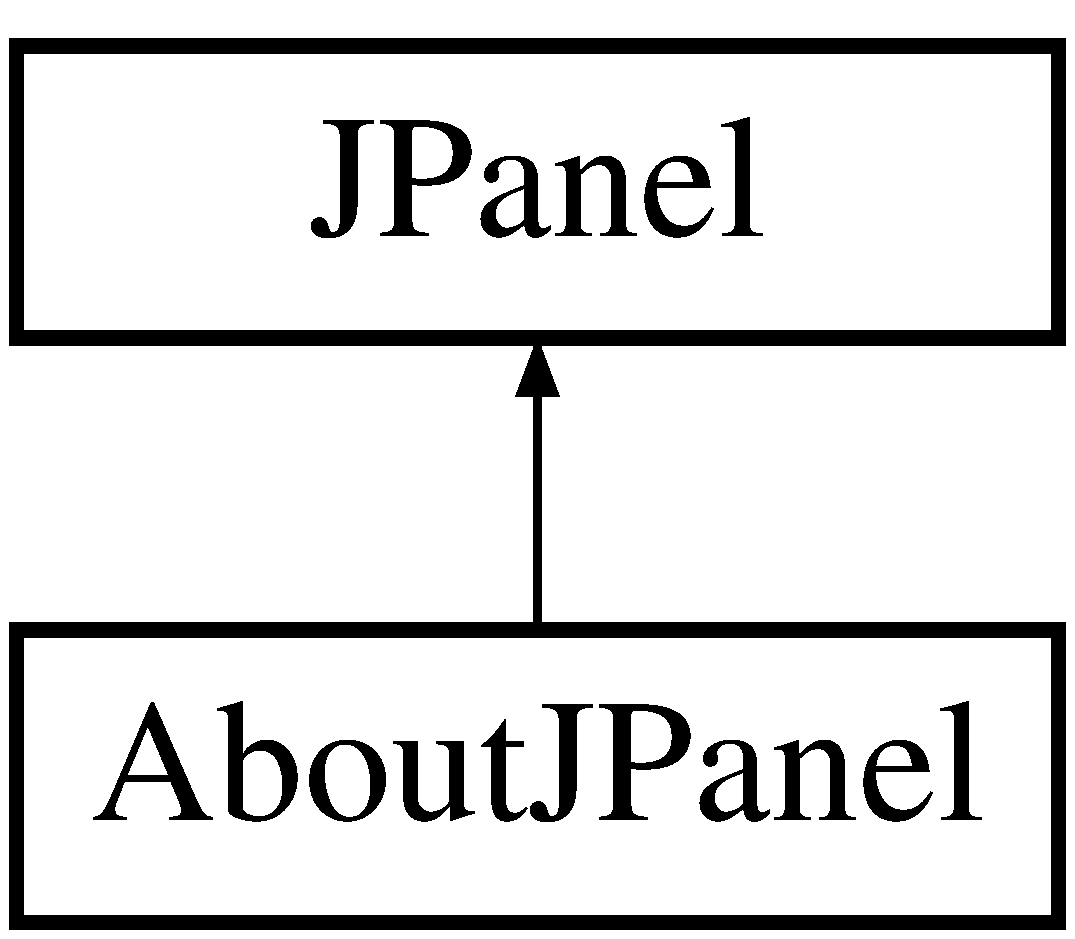
\includegraphics[height=2.000000cm]{class_about_j_panel}
\end{center}
\end{figure}
\subsection*{Public Member Functions}
\begin{DoxyCompactItemize}
\item 
\hyperlink{class_about_j_panel_a1ddd3b050eb08dd7fca8434cc00e931f}{About\-J\-Panel} ()
\item 
\hyperlink{class_about_j_panel_abb77c372f536a4a5728ad792eff280d3}{About\-J\-Panel} (boolean b)
\item 
boolean \hyperlink{class_about_j_panel_a134c5a6eee7daba01d35a1ca05ddcca1}{Set\-B\-V} (\hyperlink{class_bob_viz}{Bob\-Viz} bv)
\end{DoxyCompactItemize}
\subsection*{Static Public Member Functions}
\begin{DoxyCompactItemize}
\item 
static void \hyperlink{class_about_j_panel_ab6b17f3a162421e23430c81eac5e824f}{main} (String\mbox{[}$\,$\mbox{]} args)
\end{DoxyCompactItemize}


\subsection{Detailed Description}
This class provides the user with information about the application. 

\begin{DoxyDate}{Date}
30/04/2013 
\end{DoxyDate}
\begin{DoxySeeAlso}{See Also}
\hyperlink{_bob_viz_8java}{Bob\-Viz.\-java} 
\end{DoxySeeAlso}


\subsection{Constructor \& Destructor Documentation}
\hypertarget{class_about_j_panel_a1ddd3b050eb08dd7fca8434cc00e931f}{\index{About\-J\-Panel@{About\-J\-Panel}!About\-J\-Panel@{About\-J\-Panel}}
\index{About\-J\-Panel@{About\-J\-Panel}!AboutJPanel@{About\-J\-Panel}}
\subsubsection[{About\-J\-Panel}]{\setlength{\rightskip}{0pt plus 5cm}About\-J\-Panel.\-About\-J\-Panel (
\begin{DoxyParamCaption}
{}
\end{DoxyParamCaption}
)}}\label{class_about_j_panel_a1ddd3b050eb08dd7fca8434cc00e931f}

\begin{DoxyCode}
17                          \{
18         \textcolor{comment}{/* create dimension for AboutJPanel */}
19         Dimension size = getPreferredSize();
20         size.width = WIDTH;
21         size.height = HEIGHT;
22         \textcolor{comment}{/* set dimensions for AboutJPanel */}
23         setPreferredSize( size );
24         \textcolor{comment}{/* set border with title for AboutJPanel */} 
25         setBorder(BorderFactory.createTitledBorder(
26                 BorderFactory.createLineBorder( Color.GRAY ), \textcolor{stringliteral}{"About"}));
27         \textcolor{comment}{/* create about JLabel */}
28         JLabel about = \textcolor{keyword}{new} JLabel(\textcolor{stringliteral}{"<HTML><p>BobViz generates an array of charts"}
29                 + \textcolor{stringliteral}{" and graphs using a CSV file.</p> <p>This program was "}
30                 + \textcolor{stringliteral}{"created by group PDM1 at Swansea University, </p><p>"} +
31                 \textcolor{stringliteral}{"and then further implemented by Bradley Coles-Perkins</p></HTML>"});
32         \textcolor{comment}{/* add about JLabel to AboutJPanel */}
33         add( about );
34    
35     \}
\end{DoxyCode}
\hypertarget{class_about_j_panel_abb77c372f536a4a5728ad792eff280d3}{\index{About\-J\-Panel@{About\-J\-Panel}!About\-J\-Panel@{About\-J\-Panel}}
\index{About\-J\-Panel@{About\-J\-Panel}!AboutJPanel@{About\-J\-Panel}}
\subsubsection[{About\-J\-Panel}]{\setlength{\rightskip}{0pt plus 5cm}About\-J\-Panel.\-About\-J\-Panel (
\begin{DoxyParamCaption}
\item[{boolean}]{b}
\end{DoxyParamCaption}
)}}\label{class_about_j_panel_abb77c372f536a4a5728ad792eff280d3}

\begin{DoxyCode}
36                                     \{
37             
38     \}
\end{DoxyCode}


\subsection{Member Function Documentation}
\hypertarget{class_about_j_panel_ab6b17f3a162421e23430c81eac5e824f}{\index{About\-J\-Panel@{About\-J\-Panel}!main@{main}}
\index{main@{main}!AboutJPanel@{About\-J\-Panel}}
\subsubsection[{main}]{\setlength{\rightskip}{0pt plus 5cm}static void About\-J\-Panel.\-main (
\begin{DoxyParamCaption}
\item[{String\mbox{[}$\,$\mbox{]}}]{args}
\end{DoxyParamCaption}
)\hspace{0.3cm}{\ttfamily [static]}}}\label{class_about_j_panel_ab6b17f3a162421e23430c81eac5e824f}
This method is used for testing. 
\begin{DoxyParams}{Parameters}
{\em args} & -\/user input not used \\
\hline
\end{DoxyParams}

\begin{DoxyCode}
61                                            \{
62         \hyperlink{class_about_j_panel}{AboutJPanel} aJPan = \textcolor{keyword}{new} \hyperlink{class_about_j_panel_a1ddd3b050eb08dd7fca8434cc00e931f}{AboutJPanel}( \textcolor{keyword}{true} );
63         aJPan.\hyperlink{class_about_j_panel_a134c5a6eee7daba01d35a1ca05ddcca1}{SetBV}( null );
64     \}
\end{DoxyCode}
\hypertarget{class_about_j_panel_a134c5a6eee7daba01d35a1ca05ddcca1}{\index{About\-J\-Panel@{About\-J\-Panel}!Set\-B\-V@{Set\-B\-V}}
\index{Set\-B\-V@{Set\-B\-V}!AboutJPanel@{About\-J\-Panel}}
\subsubsection[{Set\-B\-V}]{\setlength{\rightskip}{0pt plus 5cm}boolean About\-J\-Panel.\-Set\-B\-V (
\begin{DoxyParamCaption}
\item[{{\bf Bob\-Viz}}]{bv}
\end{DoxyParamCaption}
)}}\label{class_about_j_panel_a134c5a6eee7daba01d35a1ca05ddcca1}

\begin{DoxyParams}{Parameters}
{\em bv} & -\/ a \hyperlink{class_bob_viz}{Bob\-Viz} object \\
\hline
\end{DoxyParams}
\begin{DoxyReturn}{Returns}
T\-R\-U\-E on success 
\end{DoxyReturn}

\begin{DoxyCode}
44                                       \{
45         \textcolor{keywordtype}{boolean} test = \textcolor{keyword}{true};
46         \textcolor{keywordflow}{if}( ( test == \textcolor{keyword}{true} ) && ( bv == null) ) \{
47             System.err.println( \textcolor{stringliteral}{"AboutJPanel::SetBV() ***Warning, GroupPDM2"}
48                     + \textcolor{stringliteral}{"application is null. Value sent: "} + bv );
49         \} \textcolor{keywordflow}{else} \textcolor{keywordflow}{if} ( test == \textcolor{keyword}{true} ) \{
50             System.out.println( \textcolor{stringliteral}{"AboutJPanel::SetBV() GroupPDM2"}
51                     + \textcolor{stringliteral}{"application. Value sent: "} + bv );
52         \}
53         m\_BV = bv;
54         \textcolor{keywordflow}{return} \textcolor{keyword}{true};
55     \}
\end{DoxyCode}


The documentation for this class was generated from the following file\-:\begin{DoxyCompactItemize}
\item 
\hyperlink{_about_j_panel_8java}{About\-J\-Panel.\-java}\end{DoxyCompactItemize}

\hypertarget{class_area_chart}{\section{Area\-Chart Class Reference}
\label{class_area_chart}\index{Area\-Chart@{Area\-Chart}}
}


A class that creates a single Area \hyperlink{interface_chart}{Chart} or two Area Charts visualizations from a 2\-D Array of data \textbackslash{} see \hyperlink{_graph_8java}{Graph.\-java}.  


Inheritance diagram for Area\-Chart\-:\begin{figure}[H]
\begin{center}
\leavevmode
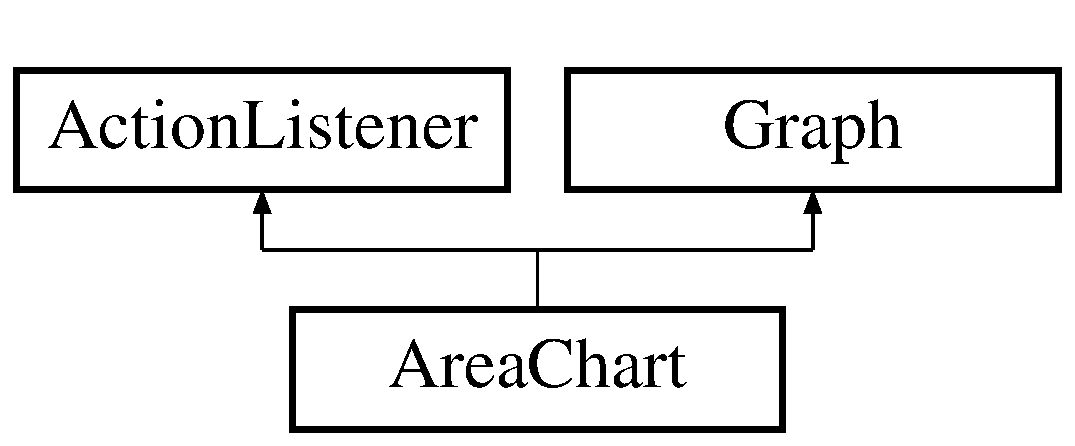
\includegraphics[height=2.000000cm]{class_area_chart}
\end{center}
\end{figure}
\subsection*{Public Member Functions}
\begin{DoxyCompactItemize}
\item 
\hyperlink{class_area_chart_ac274b6648f7927c1b21a5f2ccacdf015}{Area\-Chart} (String\mbox{[}$\,$\mbox{]}\mbox{[}$\,$\mbox{]} data, \hyperlink{class_dataset}{Dataset} dataset, \hyperlink{class_data_attribute}{Data\-Attribute} setting)
\item 
\hyperlink{class_area_chart_a89ef5b5df7dc6ca9aaa96987860bde17}{Area\-Chart} (String\mbox{[}$\,$\mbox{]}\mbox{[}$\,$\mbox{]} data, \hyperlink{class_dataset}{Dataset} dataset, \hyperlink{class_data_attribute}{Data\-Attribute} setting, String\mbox{[}$\,$\mbox{]}\mbox{[}$\,$\mbox{]} second\-Data, \hyperlink{class_dataset}{Dataset} second\-Dataset, \hyperlink{class_data_attribute}{Data\-Attribute} second\-Setting)
\item 
\hyperlink{class_area_chart_a7648545bfd821120ba898a1fbe693cd9}{Area\-Chart} (\hyperlink{class_data_attribute}{Data\-Attribute} setting)
\item 
\hyperlink{class_area_chart_a0fa85df1c042914db3ad989ebca7be30}{Area\-Chart} (\hyperlink{class_data_attribute}{Data\-Attribute} setting, \hyperlink{class_data_attribute}{Data\-Attribute} second\-Setting)
\item 
void \hyperlink{class_area_chart_a5d3648cf5639db988d10eb250058a362}{action\-Performed} (Action\-Event e)
\item 
String \hyperlink{class_area_chart_af7d8c59fa546b0f754adc9785fa4fb95}{Set\-Label\-X} (String m\-\_\-x\-Label)
\item 
String \hyperlink{class_area_chart_aa748c5e3dfc96c261f97673b5b51ecb5}{Set\-Label\-Y} (String m\-\_\-y\-Label)
\item 
String \hyperlink{class_area_chart_a0eec1001412cfee1b2d696addf56cdab}{Set\-Title} (String m\-\_\-graph\-Title)
\end{DoxyCompactItemize}
\subsection*{Static Public Member Functions}
\begin{DoxyCompactItemize}
\item 
static void \hyperlink{class_area_chart_a804e349cf99c84a448b31ab5968d266b}{main} (String\mbox{[}$\,$\mbox{]} args)
\end{DoxyCompactItemize}


\subsection{Detailed Description}
A class that creates a single Area \hyperlink{interface_chart}{Chart} or two Area Charts visualizations from a 2\-D Array of data \textbackslash{} see \hyperlink{_graph_8java}{Graph.\-java}. 

\begin{DoxyDate}{Date}
30/04/13 
\end{DoxyDate}
\begin{DoxySeeAlso}{See Also}
This class is responsible for making the Area chart It was made using J\-Free\-Chart and following examples on how to set up the Area chart It uses the \hyperlink{_graph_8java}{Graph.\-java} to return a J\-Free\-Chart 
\end{DoxySeeAlso}


\subsection{Constructor \& Destructor Documentation}
\hypertarget{class_area_chart_ac274b6648f7927c1b21a5f2ccacdf015}{\index{Area\-Chart@{Area\-Chart}!Area\-Chart@{Area\-Chart}}
\index{Area\-Chart@{Area\-Chart}!AreaChart@{Area\-Chart}}
\subsubsection[{Area\-Chart}]{\setlength{\rightskip}{0pt plus 5cm}Area\-Chart.\-Area\-Chart (
\begin{DoxyParamCaption}
\item[{String}]{data\mbox{[}$\,$\mbox{]}\mbox{[}$\,$\mbox{]}, }
\item[{{\bf Dataset}}]{dataset, }
\item[{{\bf Data\-Attribute}}]{setting}
\end{DoxyParamCaption}
)}}\label{class_area_chart_ac274b6648f7927c1b21a5f2ccacdf015}
creates a constructor taking in the following parameters\-:


\begin{DoxyParams}{Parameters}
{\em String\mbox{[}$\,$\mbox{]}\mbox{[}$\,$\mbox{]}} & data -\/ data used to create the visualisation. \\
\hline
{\em \hyperlink{class_dataset}{Dataset}} & dataset -\/ the dataset used (rows and columns) \\
\hline
{\em \hyperlink{class_data_attribute}{Data\-Attribute}} & setting -\/ Data attributes \\
\hline
\end{DoxyParams}

\begin{DoxyCode}
48                                                \{
49         
50         m\_Data = data;
51         m\_ChartTitle = setting.\hyperlink{class_data_attribute_ade9747a192ba22fe1020e874bff6a48c}{GetTitle}();
52         m\_Setting = setting;
53         m\_XLabel = setting.\hyperlink{class_data_attribute_aecb451704a87d77dd80dbad8a19099d1}{GetAxisLabelX}();
54         m\_YLabel = setting.\hyperlink{class_data_attribute_af5f68794cd0195d42135d5e48120ccc0}{GetAxisLabelY}();
55         m\_Col = dataset.\hyperlink{class_dataset_ab922bef50c8aa1531de8704731779246}{GetNoOfCols}();
56         m\_Row = dataset.\hyperlink{class_dataset_a91257a605317576e87e1c32e54739e51}{GetNoOfRows}();
57         m\_C1 = setting.\hyperlink{class_data_attribute_a0f4a54973bc44b0526f78bda945dc81b}{GetSelectedXIndex}();
58         m\_C2 = setting.\hyperlink{class_data_attribute_a82e7519853d9f470ea183dd0c39a03d6}{GetSelectedYIndex}();
59         
60         m\_XMin = setting.\hyperlink{class_data_attribute_afa9da883abc4abad5f64c045de114c50}{GetXAxisMin}();
61         m\_XMax = setting.\hyperlink{class_data_attribute_ada370712422c7cbd21b7be4a0d88caf7}{GetXAxisMax}();
62         m\_YMin = setting.\hyperlink{class_data_attribute_af0786b4de674874c0bb8ca9dbe1519c6}{GetYAxisMin}();
63         m\_YMax = setting.\hyperlink{class_data_attribute_a81243eb8f7008e05e74b0f3571d2f08d}{GetYAxisMax}();
64         
65         m\_XScale = setting.\hyperlink{class_data_attribute_a5a1de25600487aa958a19ce01151fea4}{GetXAxisScale}();
66         setting.\hyperlink{class_data_attribute_a95259727ce91efc0e0eaa28487d944c5}{GetYAxisScale}();
67         
68         createDataset(m\_Data);
69         showChart( m\_Dataset );
70     \}  
\end{DoxyCode}
\hypertarget{class_area_chart_a89ef5b5df7dc6ca9aaa96987860bde17}{\index{Area\-Chart@{Area\-Chart}!Area\-Chart@{Area\-Chart}}
\index{Area\-Chart@{Area\-Chart}!AreaChart@{Area\-Chart}}
\subsubsection[{Area\-Chart}]{\setlength{\rightskip}{0pt plus 5cm}Area\-Chart.\-Area\-Chart (
\begin{DoxyParamCaption}
\item[{String}]{data\mbox{[}$\,$\mbox{]}\mbox{[}$\,$\mbox{]}, }
\item[{{\bf Dataset}}]{dataset, }
\item[{{\bf Data\-Attribute}}]{setting, }
\item[{String}]{second\-Data\mbox{[}$\,$\mbox{]}\mbox{[}$\,$\mbox{]}, }
\item[{{\bf Dataset}}]{second\-Dataset, }
\item[{{\bf Data\-Attribute}}]{second\-Setting}
\end{DoxyParamCaption}
)}}\label{class_area_chart_a89ef5b5df7dc6ca9aaa96987860bde17}
creates a constructor taking in the following parameters\-:


\begin{DoxyParams}{Parameters}
{\em String\mbox{[}$\,$\mbox{]}\mbox{[}$\,$\mbox{]}} & data -\/ data used to create the visualisation. \\
\hline
{\em \hyperlink{class_dataset}{Dataset}} & dataset -\/ the dataset used (rows and columns) \\
\hline
{\em \hyperlink{class_data_attribute}{Data\-Attribute}} & setting -\/ Data attributes \\
\hline
{\em String\mbox{[}$\,$\mbox{]}\mbox{[}$\,$\mbox{]}} & second\-Data -\/ second data used to create the visualisation. \\
\hline
{\em \hyperlink{class_dataset}{Dataset}} & second\-Dataset -\/ the second dataset used (rows and columns) \\
\hline
{\em \hyperlink{class_data_attribute}{Data\-Attribute}} & second\-Setting -\/ Second Data attributes \\
\hline
\end{DoxyParams}

\begin{DoxyCode}
83                                           \{
84     
85         m\_Data = data;
86         m\_ChartTitle = setting.\hyperlink{class_data_attribute_ade9747a192ba22fe1020e874bff6a48c}{GetTitle}();
87         m\_Setting = setting;
88         m\_XLabel = setting.\hyperlink{class_data_attribute_aecb451704a87d77dd80dbad8a19099d1}{GetAxisLabelX}();
89         m\_YLabel = setting.\hyperlink{class_data_attribute_af5f68794cd0195d42135d5e48120ccc0}{GetAxisLabelY}();
90         m\_Col = dataset.\hyperlink{class_dataset_ab922bef50c8aa1531de8704731779246}{GetNoOfCols}();
91         m\_Row = dataset.\hyperlink{class_dataset_a91257a605317576e87e1c32e54739e51}{GetNoOfRows}();
92         m\_C1 = setting.\hyperlink{class_data_attribute_a0f4a54973bc44b0526f78bda945dc81b}{GetSelectedXIndex}();
93         m\_C2 = setting.\hyperlink{class_data_attribute_a82e7519853d9f470ea183dd0c39a03d6}{GetSelectedYIndex}();
94         
95         m\_XMin = setting.\hyperlink{class_data_attribute_afa9da883abc4abad5f64c045de114c50}{GetXAxisMin}();
96         m\_XMax = setting.\hyperlink{class_data_attribute_ada370712422c7cbd21b7be4a0d88caf7}{GetXAxisMax}();
97         m\_YMin = setting.\hyperlink{class_data_attribute_af0786b4de674874c0bb8ca9dbe1519c6}{GetYAxisMin}();
98         m\_YMax = setting.\hyperlink{class_data_attribute_a81243eb8f7008e05e74b0f3571d2f08d}{GetYAxisMax}();
99         
100         m\_XScale = setting.\hyperlink{class_data_attribute_a5a1de25600487aa958a19ce01151fea4}{GetXAxisScale}();
101         setting.\hyperlink{class_data_attribute_a95259727ce91efc0e0eaa28487d944c5}{GetYAxisScale}();
102         
103         m\_SecondData = secondData;
104         m\_SecondChartTitle = secondSetting.\hyperlink{class_data_attribute_a4079522c93025fce7569eaed585f4aeb}{GetSecondTitle}();
105         m\_SecondSetting = secondSetting;
106         m\_SecondXLabel = secondSetting.\hyperlink{class_data_attribute_a8ace4cb1fee9e2abeabe3efc9a190c8f}{GetSecondAxisLabelX}();
107         m\_SecondYLabel = secondSetting.\hyperlink{class_data_attribute_a6efb7e067317898feefbbf6bd472b998}{GetSecondAxisLabelY}();
108         m\_SecondCol = secondDataset.\hyperlink{class_dataset_ab922bef50c8aa1531de8704731779246}{GetNoOfCols}();
109         m\_SecondRow = secondDataset.\hyperlink{class_dataset_a91257a605317576e87e1c32e54739e51}{GetNoOfRows}();
110         m\_SecondC1 = secondSetting.\hyperlink{class_data_attribute_a7f501790eee650ddf9ac17c4f63a3995}{GetSecondSelectedXIndex}();
111         m\_SecondC2 = secondSetting.\hyperlink{class_data_attribute_a6f61ad05915f4aa31ad3dba00596da64}{GetSecondSelectedYIndex}();
112 
113         secondSetting.\hyperlink{class_data_attribute_a95259727ce91efc0e0eaa28487d944c5}{GetYAxisScale}();
114         
115         createDataset(m\_Data);
116         createSecondDataset(m\_SecondData);
117         showChart( m\_Dataset, m\_SecondDataset );
118     \} 
\end{DoxyCode}
\hypertarget{class_area_chart_a7648545bfd821120ba898a1fbe693cd9}{\index{Area\-Chart@{Area\-Chart}!Area\-Chart@{Area\-Chart}}
\index{Area\-Chart@{Area\-Chart}!AreaChart@{Area\-Chart}}
\subsubsection[{Area\-Chart}]{\setlength{\rightskip}{0pt plus 5cm}Area\-Chart.\-Area\-Chart (
\begin{DoxyParamCaption}
\item[{{\bf Data\-Attribute}}]{setting}
\end{DoxyParamCaption}
)}}\label{class_area_chart_a7648545bfd821120ba898a1fbe693cd9}
constructor for J\-Unit Tests 
\begin{DoxyParams}{Parameters}
{\em setting} & \\
\hline
\end{DoxyParams}

\begin{DoxyCode}
124                                             \{       
125         m\_ChartTitle = setting.\hyperlink{class_data_attribute_ade9747a192ba22fe1020e874bff6a48c}{GetTitle}();
126          m\_Setting = setting;
127          m\_XLabel = setting.\hyperlink{class_data_attribute_aecb451704a87d77dd80dbad8a19099d1}{GetAxisLabelX}();
128          m\_YLabel = setting.\hyperlink{class_data_attribute_af5f68794cd0195d42135d5e48120ccc0}{GetAxisLabelY}();
129          m\_C1 = setting.\hyperlink{class_data_attribute_a0f4a54973bc44b0526f78bda945dc81b}{GetSelectedXIndex}();
130          m\_C2 = setting.\hyperlink{class_data_attribute_a82e7519853d9f470ea183dd0c39a03d6}{GetSelectedYIndex}();
131     \}
\end{DoxyCode}
\hypertarget{class_area_chart_a0fa85df1c042914db3ad989ebca7be30}{\index{Area\-Chart@{Area\-Chart}!Area\-Chart@{Area\-Chart}}
\index{Area\-Chart@{Area\-Chart}!AreaChart@{Area\-Chart}}
\subsubsection[{Area\-Chart}]{\setlength{\rightskip}{0pt plus 5cm}Area\-Chart.\-Area\-Chart (
\begin{DoxyParamCaption}
\item[{{\bf Data\-Attribute}}]{setting, }
\item[{{\bf Data\-Attribute}}]{second\-Setting}
\end{DoxyParamCaption}
)}}\label{class_area_chart_a0fa85df1c042914db3ad989ebca7be30}
second empty constructor for J\-Unit Tests 
\begin{DoxyParams}{Parameters}
{\em setting} & \\
\hline
{\em second\-Setting} & \\
\hline
\end{DoxyParams}

\begin{DoxyCode}
137                                                                          \{       
138         m\_ChartTitle = setting.\hyperlink{class_data_attribute_ade9747a192ba22fe1020e874bff6a48c}{GetTitle}();
139         m\_Setting = setting;
140         m\_XLabel = setting.\hyperlink{class_data_attribute_aecb451704a87d77dd80dbad8a19099d1}{GetAxisLabelX}();
141         m\_YLabel = setting.\hyperlink{class_data_attribute_af5f68794cd0195d42135d5e48120ccc0}{GetAxisLabelY}();
142         m\_C1 = setting.\hyperlink{class_data_attribute_a0f4a54973bc44b0526f78bda945dc81b}{GetSelectedXIndex}();
143         m\_C2 = setting.\hyperlink{class_data_attribute_a82e7519853d9f470ea183dd0c39a03d6}{GetSelectedYIndex}();
144         m\_SecondChartTitle = secondSetting.\hyperlink{class_data_attribute_a4079522c93025fce7569eaed585f4aeb}{GetSecondTitle}();
145         m\_SecondSetting = secondSetting;
146         m\_SecondXLabel = secondSetting.\hyperlink{class_data_attribute_a8ace4cb1fee9e2abeabe3efc9a190c8f}{GetSecondAxisLabelX}();
147         m\_SecondYLabel = secondSetting.\hyperlink{class_data_attribute_a6efb7e067317898feefbbf6bd472b998}{GetSecondAxisLabelY}();
148         m\_SecondC1 = secondSetting.\hyperlink{class_data_attribute_a7f501790eee650ddf9ac17c4f63a3995}{GetSecondSelectedXIndex}();
149         m\_SecondC2 = secondSetting.\hyperlink{class_data_attribute_a6f61ad05915f4aa31ad3dba00596da64}{GetSecondSelectedYIndex}();
150     \}
\end{DoxyCode}


\subsection{Member Function Documentation}
\hypertarget{class_area_chart_a5d3648cf5639db988d10eb250058a362}{\index{Area\-Chart@{Area\-Chart}!action\-Performed@{action\-Performed}}
\index{action\-Performed@{action\-Performed}!AreaChart@{Area\-Chart}}
\subsubsection[{action\-Performed}]{\setlength{\rightskip}{0pt plus 5cm}void Area\-Chart.\-action\-Performed (
\begin{DoxyParamCaption}
\item[{Action\-Event}]{e}
\end{DoxyParamCaption}
)}}\label{class_area_chart_a5d3648cf5639db988d10eb250058a362}
allows user to select the colour of the points on the area chart 
\begin{DoxyCode}
155                                                  \{
156         \textcolor{keywordflow}{if}( e.getSource() == m\_ColChangeButton ) \{
157             \hyperlink{class_colour_map}{ColourMap} cM = \textcolor{keyword}{new} \hyperlink{class_colour_map}{ColourMap}();
158             cM.\hyperlink{class_colour_map_a9f696ea699b7fc471bb2dde6f1d1ce09}{SetupData}( m\_Plot.getSeriesCount(), 
159                           m\_Renderer );
160             cM.setVisible( \textcolor{keyword}{false} );
161         \}
162     \}
\end{DoxyCode}
\hypertarget{class_area_chart_a804e349cf99c84a448b31ab5968d266b}{\index{Area\-Chart@{Area\-Chart}!main@{main}}
\index{main@{main}!AreaChart@{Area\-Chart}}
\subsubsection[{main}]{\setlength{\rightskip}{0pt plus 5cm}static void Area\-Chart.\-main (
\begin{DoxyParamCaption}
\item[{String\mbox{[}$\,$\mbox{]}}]{args}
\end{DoxyParamCaption}
)\hspace{0.3cm}{\ttfamily [static]}}}\label{class_area_chart_a804e349cf99c84a448b31ab5968d266b}
main method to carry out J\-Unit Tests 
\begin{DoxyCode}
473                                              \{
474         \hyperlink{class_data_attribute}{DataAttribute} test = \hyperlink{class_data_attribute}{DataAttribute}.
      \hyperlink{class_data_attribute_a9c7a1923698c1530fa38c959596199bc}{GetTestDataAttribute}();
475         \hyperlink{class_area_chart}{AreaChart} areaChartTest = \textcolor{keyword}{new} \hyperlink{class_area_chart_ac274b6648f7927c1b21a5f2ccacdf015}{AreaChart}(test);
476         
477         \textcolor{keyword}{final} XYDataset testDataset = createDataset();
478         areaChartTest.showChart(testDataset);
479         
480         \hyperlink{class_data_attribute}{DataAttribute} secondTest = \hyperlink{class_data_attribute}{DataAttribute}.
      \hyperlink{class_data_attribute_a9c7a1923698c1530fa38c959596199bc}{GetTestDataAttribute}();
481         \hyperlink{class_area_chart}{AreaChart} secondAreaChartTest = \textcolor{keyword}{new} \hyperlink{class_area_chart_ac274b6648f7927c1b21a5f2ccacdf015}{AreaChart}(secondTest);
482         
483         \textcolor{keyword}{final} XYDataset secondTestDataset = createSecondDataset();
484         secondAreaChartTest.showChart(testDataset, secondTestDataset);
485     \}
\end{DoxyCode}
\hypertarget{class_area_chart_af7d8c59fa546b0f754adc9785fa4fb95}{\index{Area\-Chart@{Area\-Chart}!Set\-Label\-X@{Set\-Label\-X}}
\index{Set\-Label\-X@{Set\-Label\-X}!AreaChart@{Area\-Chart}}
\subsubsection[{Set\-Label\-X}]{\setlength{\rightskip}{0pt plus 5cm}String Area\-Chart.\-Set\-Label\-X (
\begin{DoxyParamCaption}
\item[{String}]{m\-\_\-x\-Label}
\end{DoxyParamCaption}
)}}\label{class_area_chart_af7d8c59fa546b0f754adc9785fa4fb95}

\begin{DoxyParams}{Parameters}
{\em m\-\_\-x\-Label} & -\/ the x axis label passed from users to the graph \\
\hline
\end{DoxyParams}
\begin{DoxyReturn}{Returns}
m\-\_\-label\-X -\/ returns the user's x label value 
\end{DoxyReturn}

\begin{DoxyCode}
169                                                \{
170     String m\_labelX = m\_xLabel;
171         
172         \textcolor{keywordtype}{boolean} test = \textcolor{keyword}{true};
173         \textcolor{keywordflow}{if} ( ( ( m\_xLabel.isEmpty() )||( m\_xLabel.length() > MAX\_LABEL\_LENGTH ) ) 
174                  && ( test == true ) ) \{
175             System.err.println( \textcolor{stringliteral}{"AreaChart::SetLabelX() "} + 
176                                 m\_xLabel );
177         \}
178         \textcolor{keywordflow}{return} m\_labelX;
179     \}
\end{DoxyCode}
\hypertarget{class_area_chart_aa748c5e3dfc96c261f97673b5b51ecb5}{\index{Area\-Chart@{Area\-Chart}!Set\-Label\-Y@{Set\-Label\-Y}}
\index{Set\-Label\-Y@{Set\-Label\-Y}!AreaChart@{Area\-Chart}}
\subsubsection[{Set\-Label\-Y}]{\setlength{\rightskip}{0pt plus 5cm}String Area\-Chart.\-Set\-Label\-Y (
\begin{DoxyParamCaption}
\item[{String}]{m\-\_\-y\-Label}
\end{DoxyParamCaption}
)}}\label{class_area_chart_aa748c5e3dfc96c261f97673b5b51ecb5}

\begin{DoxyParams}{Parameters}
{\em m\-\_\-y\-Label} & -\/ the y axis label passed from users to the graph \\
\hline
\end{DoxyParams}
\begin{DoxyReturn}{Returns}
m\-\_\-label\-Y -\/ returns the user's y label value 
\end{DoxyReturn}

\begin{DoxyCode}
186                                                \{
187         String m\_labelY = m\_yLabel;
188         
189         \textcolor{keywordtype}{boolean} test = \textcolor{keyword}{true};
190         \textcolor{keywordflow}{if} ( ( ( m\_yLabel.isEmpty() )||( m\_yLabel.length() > MAX\_LABEL\_LENGTH ) ) 
191                  && ( test == true ) ) \{
192             System.err.println( \textcolor{stringliteral}{"AreaChart::SetLabelY() "} + 
193                                 m\_yLabel );
194         \}
195         \textcolor{keywordflow}{return} m\_labelY;
196     \}
\end{DoxyCode}
\hypertarget{class_area_chart_a0eec1001412cfee1b2d696addf56cdab}{\index{Area\-Chart@{Area\-Chart}!Set\-Title@{Set\-Title}}
\index{Set\-Title@{Set\-Title}!AreaChart@{Area\-Chart}}
\subsubsection[{Set\-Title}]{\setlength{\rightskip}{0pt plus 5cm}String Area\-Chart.\-Set\-Title (
\begin{DoxyParamCaption}
\item[{String}]{m\-\_\-graph\-Title}
\end{DoxyParamCaption}
)}}\label{class_area_chart_a0eec1001412cfee1b2d696addf56cdab}

\begin{DoxyParams}{Parameters}
{\em m\-\_\-graph\-Title} & -\/ the title passed from users to the graph \\
\hline
\end{DoxyParams}
\begin{DoxyReturn}{Returns}
m\-\_\-label\-Y -\/ returns the user's title value 
\end{DoxyReturn}

\begin{DoxyCode}
203                                                   \{
204         String m\_title = m\_graphTitle;
205         
206         \textcolor{keywordtype}{boolean} test = \textcolor{keyword}{true};
207         \textcolor{keywordflow}{if} ( ( ( m\_graphTitle.isEmpty() )||( m\_graphTitle.length() > MAX\_TITLE\_LENGTH ) ) 
208                  && ( test == true ) ) \{
209             System.err.println( \textcolor{stringliteral}{"AreaChart::SetTitle() "} + 
210                                 m\_graphTitle );
211         \}   
212         \textcolor{keywordflow}{return} m\_title;
213     \} 
\end{DoxyCode}


The documentation for this class was generated from the following file\-:\begin{DoxyCompactItemize}
\item 
\hyperlink{_area_chart_8java}{Area\-Chart.\-java}\end{DoxyCompactItemize}

\hypertarget{class_bob_viz}{\section{Bob\-Viz Class Reference}
\label{class_bob_viz}\index{Bob\-Viz@{Bob\-Viz}}
}


This class provides the user with a simple G\-U\-I system. It initiates all instances used throughout the application.  


Inheritance diagram for Bob\-Viz\-:\begin{figure}[H]
\begin{center}
\leavevmode
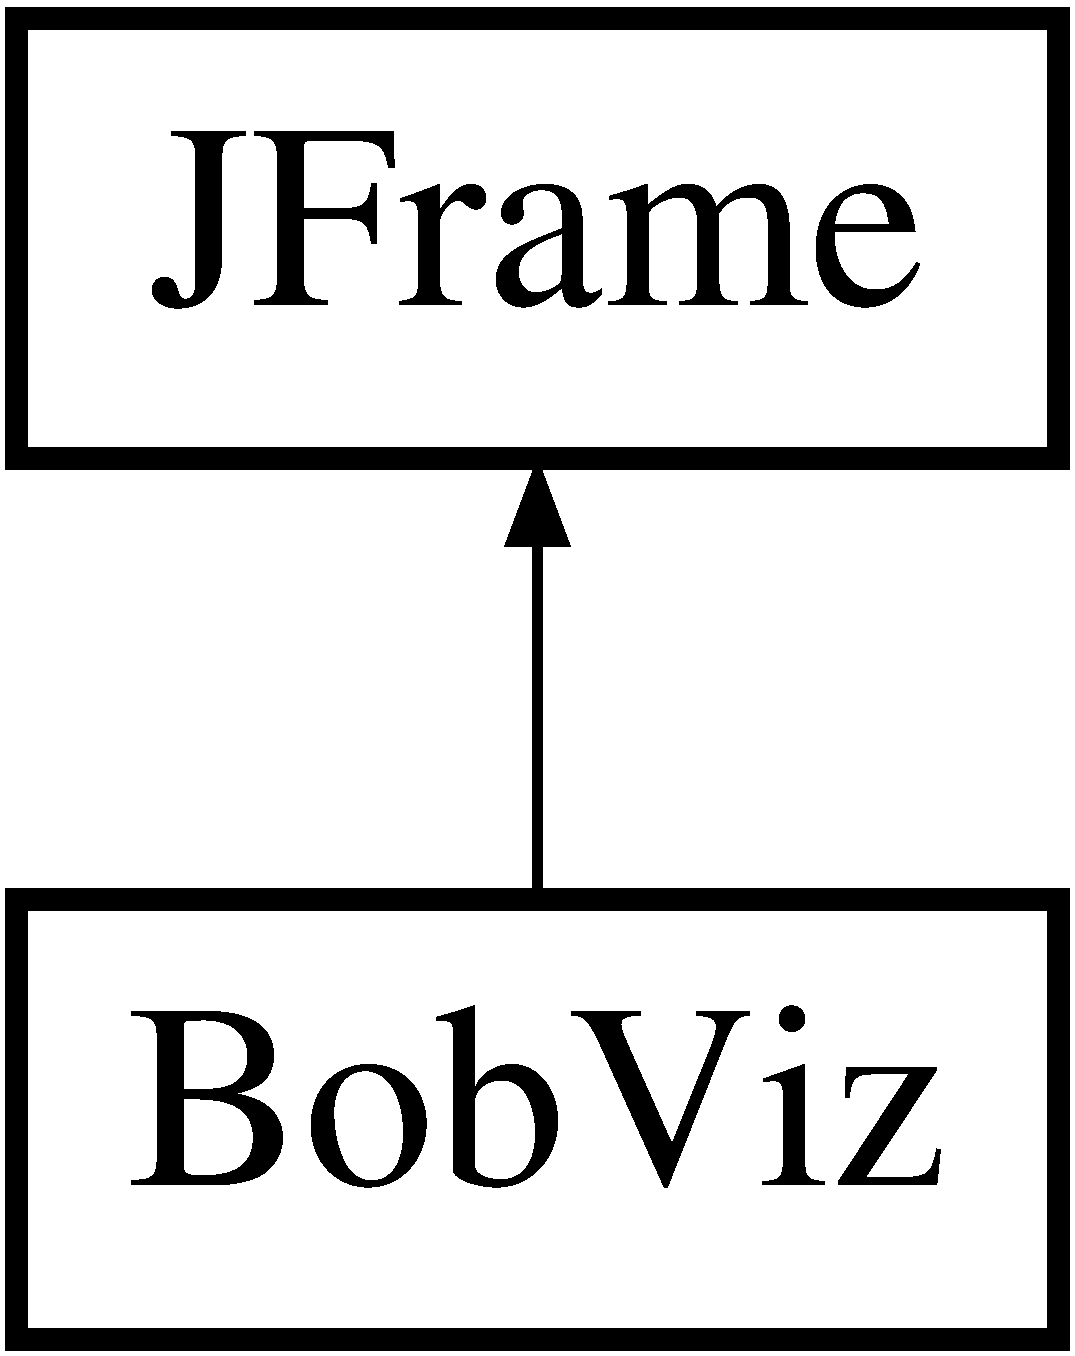
\includegraphics[height=2.000000cm]{class_bob_viz}
\end{center}
\end{figure}
\subsection*{Public Member Functions}
\begin{DoxyCompactItemize}
\item 
\hyperlink{class_bob_viz_a362406b3528e341eb5f8339e28ae7a17}{Bob\-Viz} ()
\item 
boolean \hyperlink{class_bob_viz_a76ae5d60149c159834708456b28d9222}{Set\-B\-V} (\hyperlink{class_bob_viz}{Bob\-Viz} bv)
\item 
\hyperlink{class_about_j_panel}{About\-J\-Panel} \hyperlink{class_bob_viz_aac948a35c1e508b168aad19efba2053d}{Get\-About\-J\-Pan} ()
\item 
\hyperlink{class_data_attribute}{Data\-Attribute} \hyperlink{class_bob_viz_acc980a6db181f9ace3279e5dd3fd23b8}{Get\-Data\-Attribute} ()
\item 
\hyperlink{class_data_attribute}{Data\-Attribute} \hyperlink{class_bob_viz_a3bbdcd2d94adf10bfd50ae6eefe90717}{Get\-Second\-Data\-Attribute} ()
\item 
\hyperlink{class_dataset}{Dataset} \hyperlink{class_bob_viz_ab8866566b53e78c66e29a4d68406b860}{Get\-Dataset} ()
\item 
\hyperlink{class_dataset}{Dataset} \hyperlink{class_bob_viz_a2826dca37585b5effe3a2f2222f17ada}{Get\-Second\-Dataset} ()
\item 
\hyperlink{class_import_j_panel}{Import\-J\-Panel} \hyperlink{class_bob_viz_a93eb7320a1f76d531874cd0bfe5c6b71}{Get\-Import\-J\-Pan} ()
\item 
\hyperlink{class_table}{Table} \hyperlink{class_bob_viz_a52e7c8f67daa12f4882a396e557e8ed4}{Get\-Table\-J\-Pan} ()
\item 
\hyperlink{class_table}{Table} \hyperlink{class_bob_viz_afce2ebaa330fc80c477b7156fc5bc32e}{Get\-Second\-Table\-J\-Pan} ()
\item 
\hyperlink{class_setting_j_panel}{Setting\-J\-Panel} \hyperlink{class_bob_viz_a10dab616869fe644d16c2ccf78627af5}{Get\-Setting\-J\-Pan} ()
\item 
\hyperlink{class_more_setting_j_panel}{More\-Setting\-J\-Panel} \hyperlink{class_bob_viz_a26ad68d96e3524c2eb53425f59deab8a}{Get\-More\-Setting\-J\-Pan} ()
\item 
\hyperlink{class_viz_type_j_panel}{Viz\-Type\-J\-Panel} \hyperlink{class_bob_viz_a35af0807f9fca7a0773ce8217b2065c7}{Get\-Viz\-Type\-J\-Pan} ()
\item 
\hyperlink{class_status_j_panel}{Status\-J\-Panel} \hyperlink{class_bob_viz_a31b771c2acf2b72658beb4f3eecab892}{Get\-Status\-J\-Pan} ()
\item 
\hyperlink{class_selection_viz_j_panel}{Selection\-Viz\-J\-Panel} \hyperlink{class_bob_viz_a4b1e563e0fa60594fa0beb1d50438824}{Get\-Generate\-Viz\-J\-Pan} ()
\item 
\hyperlink{class_visualisation}{Visualisation} \hyperlink{class_bob_viz_a239767cb7f7f32710826f9efc91b4af9}{Get\-Viz} ()
\end{DoxyCompactItemize}


\subsection{Detailed Description}
This class provides the user with a simple G\-U\-I system. It initiates all instances used throughout the application. 

\begin{DoxyDate}{Date}
-\/30/03/2013 
\end{DoxyDate}


\subsection{Constructor \& Destructor Documentation}
\hypertarget{class_bob_viz_a362406b3528e341eb5f8339e28ae7a17}{\index{Bob\-Viz@{Bob\-Viz}!Bob\-Viz@{Bob\-Viz}}
\index{Bob\-Viz@{Bob\-Viz}!BobViz@{Bob\-Viz}}
\subsubsection[{Bob\-Viz}]{\setlength{\rightskip}{0pt plus 5cm}Bob\-Viz.\-Bob\-Viz (
\begin{DoxyParamCaption}
{}
\end{DoxyParamCaption}
)}}\label{class_bob_viz_a362406b3528e341eb5f8339e28ae7a17}

\begin{DoxyCode}
25                     \{
26         \textcolor{comment}{/* create new JPanel which will hold all GUI components */}
27         JPanel top = \textcolor{keyword}{new} JPanel();
28         \textcolor{comment}{/* create a new JPanel which will hold the current status of program */}
29         m\_StatusJPan = \textcolor{keyword}{new} \hyperlink{class_status_j_panel}{StatusJPanel}();
30         
31         \textcolor{comment}{/* set frame title for BobViz */}
32         setTitle( FRAME\_TITLE );
33         \textcolor{comment}{/* set frame height and width for BobViz */}
34         setSize( FRAME\_WIDTH, FRAME\_HEIGHT );
35         setResizable( \textcolor{keyword}{false} );
36         setLayout( \textcolor{keyword}{new} BorderLayout() );
37         setDefaultCloseOperation( JFrame.EXIT\_ON\_CLOSE );
38 
39         \textcolor{comment}{/* create new menu bar for BobViz */}
40         m\_MenuBar = \textcolor{keyword}{new} JMenuBar();
41 
42         \textcolor{comment}{/* create new menu */}
43         m\_FileMenu = \textcolor{keyword}{new} JMenu( FILE\_MENU );
44 
45         \textcolor{comment}{/* create new menu items */}
46         m\_ImportCSVItem = \textcolor{keyword}{new} JMenuItem( FILE\_IMPORTCSV );
47         m\_ExitItem = \textcolor{keyword}{new} JMenuItem( FILE\_EXIT );
48         m\_HelpConItem = \textcolor{keyword}{new} JMenuItem( FILE\_HELPCON );
49         
50         \textcolor{comment}{/* add menu items to file menu */}
51         m\_FileMenu.add( m\_ImportCSVItem );
52         m\_FileMenu.add( m\_ExitItem );
53 
54         \textcolor{comment}{/* make new help menu */}
55         m\_HelpMenu = \textcolor{keyword}{new} JMenu( FILE\_HELP );
56         
57         \textcolor{comment}{/* add menu bars to menu */}
58         m\_MenuBar.add( m\_FileMenu );
59         m\_MenuBar.add( m\_HelpMenu );
60         
61         \textcolor{comment}{/* make new help content menu item */}
62         \textcolor{comment}{/* add helpConItem to menu */}
63         m\_HelpMenu.add( m\_HelpConItem );
64         
65         \textcolor{comment}{/* add menu bar to BobViz */}
66         setJMenuBar( m\_MenuBar );
67         
68         \textcolor{comment}{/* add the mouse listener for menu */}
69         MouseListener popupListener = \textcolor{keyword}{new} PopupListener();
70         m\_ImportCSVItem.addMouseListener( popupListener );
71         m\_ExitItem.addMouseListener( popupListener );
72         
73         \textcolor{comment}{/* create new logo for BobViz */}
74         ImageIcon bvIcon = \textcolor{keyword}{new} ImageIcon( LOGO\_DIR );
75         \textcolor{comment}{/* add icon to JLabel */}
76         JLabel bobTitleJPan = \textcolor{keyword}{new} JLabel( bvIcon );
77         
78         \textcolor{comment}{/* make new instances of all panels */}
79         m\_AboutJPan = \textcolor{keyword}{new} \hyperlink{class_about_j_panel}{AboutJPanel}();
80         m\_ImportJPan = \textcolor{keyword}{new} \hyperlink{class_import_j_panel}{ImportJPanel}();
81         m\_VizTypeJPan = \textcolor{keyword}{new} \hyperlink{class_viz_type_j_panel}{VizTypeJPanel}();
82         m\_SettingJPan = \textcolor{keyword}{new} \hyperlink{class_setting_j_panel}{SettingJPanel}();
83         m\_SelectionVizJPan = \textcolor{keyword}{new} \hyperlink{class_selection_viz_j_panel}{SelectionVizJPanel}();
84         
85         \textcolor{comment}{/* set top panel with FlowLayout layout */}
86         top.setLayout( \textcolor{keyword}{new} FlowLayout( FlowLayout.CENTER ) );
87         \textcolor{comment}{/* add all panels and titles to top JPanel */}
88         top.add( bobTitleJPan );
89         top.add( m\_AboutJPan );
90         top.add( m\_ImportJPan );
91         top.add( m\_VizTypeJPan );
92         top.add( m\_SettingJPan );
93         top.add( m\_SelectionVizJPan );
94         
95         \textcolor{comment}{/* add top and m\_StatusJPan to BobViz */}
96         add( top, BorderLayout.CENTER );
97         add( m\_StatusJPan, BorderLayout.SOUTH );
98         
99         setVisible( \textcolor{keyword}{true} );
100   
101     \}
\end{DoxyCode}


\subsection{Member Function Documentation}
\hypertarget{class_bob_viz_aac948a35c1e508b168aad19efba2053d}{\index{Bob\-Viz@{Bob\-Viz}!Get\-About\-J\-Pan@{Get\-About\-J\-Pan}}
\index{Get\-About\-J\-Pan@{Get\-About\-J\-Pan}!BobViz@{Bob\-Viz}}
\subsubsection[{Get\-About\-J\-Pan}]{\setlength{\rightskip}{0pt plus 5cm}{\bf About\-J\-Panel} Bob\-Viz.\-Get\-About\-J\-Pan (
\begin{DoxyParamCaption}
{}
\end{DoxyParamCaption}
)}}\label{class_bob_viz_aac948a35c1e508b168aad19efba2053d}
\begin{DoxyReturn}{Returns}
the \hyperlink{class_about_j_panel}{About\-J\-Panel} instance 
\end{DoxyReturn}

\begin{DoxyCode}
123                                       \{
124         \textcolor{keywordflow}{return} m\_AboutJPan;
125     \}
\end{DoxyCode}
\hypertarget{class_bob_viz_acc980a6db181f9ace3279e5dd3fd23b8}{\index{Bob\-Viz@{Bob\-Viz}!Get\-Data\-Attribute@{Get\-Data\-Attribute}}
\index{Get\-Data\-Attribute@{Get\-Data\-Attribute}!BobViz@{Bob\-Viz}}
\subsubsection[{Get\-Data\-Attribute}]{\setlength{\rightskip}{0pt plus 5cm}{\bf Data\-Attribute} Bob\-Viz.\-Get\-Data\-Attribute (
\begin{DoxyParamCaption}
{}
\end{DoxyParamCaption}
)}}\label{class_bob_viz_acc980a6db181f9ace3279e5dd3fd23b8}
\begin{DoxyReturn}{Returns}
the \hyperlink{class_data_attribute}{Data\-Attribute} instance 
\end{DoxyReturn}

\begin{DoxyCode}
130                                             \{
131         \textcolor{keywordflow}{return} m\_DataAttribute;
132     \}
\end{DoxyCode}
\hypertarget{class_bob_viz_ab8866566b53e78c66e29a4d68406b860}{\index{Bob\-Viz@{Bob\-Viz}!Get\-Dataset@{Get\-Dataset}}
\index{Get\-Dataset@{Get\-Dataset}!BobViz@{Bob\-Viz}}
\subsubsection[{Get\-Dataset}]{\setlength{\rightskip}{0pt plus 5cm}{\bf Dataset} Bob\-Viz.\-Get\-Dataset (
\begin{DoxyParamCaption}
{}
\end{DoxyParamCaption}
)}}\label{class_bob_viz_ab8866566b53e78c66e29a4d68406b860}
\begin{DoxyReturn}{Returns}
the \hyperlink{class_dataset}{Dataset} instance 
\end{DoxyReturn}

\begin{DoxyCode}
144                                 \{
145         \textcolor{keywordflow}{return} m\_Dataset;
146     \}
\end{DoxyCode}
\hypertarget{class_bob_viz_a4b1e563e0fa60594fa0beb1d50438824}{\index{Bob\-Viz@{Bob\-Viz}!Get\-Generate\-Viz\-J\-Pan@{Get\-Generate\-Viz\-J\-Pan}}
\index{Get\-Generate\-Viz\-J\-Pan@{Get\-Generate\-Viz\-J\-Pan}!BobViz@{Bob\-Viz}}
\subsubsection[{Get\-Generate\-Viz\-J\-Pan}]{\setlength{\rightskip}{0pt plus 5cm}{\bf Selection\-Viz\-J\-Panel} Bob\-Viz.\-Get\-Generate\-Viz\-J\-Pan (
\begin{DoxyParamCaption}
{}
\end{DoxyParamCaption}
)}}\label{class_bob_viz_a4b1e563e0fa60594fa0beb1d50438824}
\begin{DoxyReturn}{Returns}
the Generate\-Viz\-J\-Panel instance 
\end{DoxyReturn}

\begin{DoxyCode}
211                                                    \{
212         \textcolor{keywordflow}{return} m\_SelectionVizJPan;
213     \}
\end{DoxyCode}
\hypertarget{class_bob_viz_a93eb7320a1f76d531874cd0bfe5c6b71}{\index{Bob\-Viz@{Bob\-Viz}!Get\-Import\-J\-Pan@{Get\-Import\-J\-Pan}}
\index{Get\-Import\-J\-Pan@{Get\-Import\-J\-Pan}!BobViz@{Bob\-Viz}}
\subsubsection[{Get\-Import\-J\-Pan}]{\setlength{\rightskip}{0pt plus 5cm}{\bf Import\-J\-Panel} Bob\-Viz.\-Get\-Import\-J\-Pan (
\begin{DoxyParamCaption}
{}
\end{DoxyParamCaption}
)}}\label{class_bob_viz_a93eb7320a1f76d531874cd0bfe5c6b71}
\begin{DoxyReturn}{Returns}
the \hyperlink{class_import_j_panel}{Import\-J\-Panel} instance 
\end{DoxyReturn}

\begin{DoxyCode}
158                                         \{
159         \textcolor{keywordflow}{return} m\_ImportJPan;
160     \}
\end{DoxyCode}
\hypertarget{class_bob_viz_a26ad68d96e3524c2eb53425f59deab8a}{\index{Bob\-Viz@{Bob\-Viz}!Get\-More\-Setting\-J\-Pan@{Get\-More\-Setting\-J\-Pan}}
\index{Get\-More\-Setting\-J\-Pan@{Get\-More\-Setting\-J\-Pan}!BobViz@{Bob\-Viz}}
\subsubsection[{Get\-More\-Setting\-J\-Pan}]{\setlength{\rightskip}{0pt plus 5cm}{\bf More\-Setting\-J\-Panel} Bob\-Viz.\-Get\-More\-Setting\-J\-Pan (
\begin{DoxyParamCaption}
{}
\end{DoxyParamCaption}
)}}\label{class_bob_viz_a26ad68d96e3524c2eb53425f59deab8a}
\begin{DoxyReturn}{Returns}
the \hyperlink{class_more_setting_j_panel}{More\-Setting\-J\-Panel} instance 
\end{DoxyReturn}

\begin{DoxyCode}
190                                                   \{
191         \textcolor{keywordflow}{return} m\_MoreSettingJPan;
192     \}
\end{DoxyCode}
\hypertarget{class_bob_viz_a3bbdcd2d94adf10bfd50ae6eefe90717}{\index{Bob\-Viz@{Bob\-Viz}!Get\-Second\-Data\-Attribute@{Get\-Second\-Data\-Attribute}}
\index{Get\-Second\-Data\-Attribute@{Get\-Second\-Data\-Attribute}!BobViz@{Bob\-Viz}}
\subsubsection[{Get\-Second\-Data\-Attribute}]{\setlength{\rightskip}{0pt plus 5cm}{\bf Data\-Attribute} Bob\-Viz.\-Get\-Second\-Data\-Attribute (
\begin{DoxyParamCaption}
{}
\end{DoxyParamCaption}
)}}\label{class_bob_viz_a3bbdcd2d94adf10bfd50ae6eefe90717}
\begin{DoxyReturn}{Returns}
the second \hyperlink{class_data_attribute}{Data\-Attribute} instance 
\end{DoxyReturn}

\begin{DoxyCode}
137                                                   \{
138         \textcolor{keywordflow}{return} m\_SecondDataAttribute;
139     \}
\end{DoxyCode}
\hypertarget{class_bob_viz_a2826dca37585b5effe3a2f2222f17ada}{\index{Bob\-Viz@{Bob\-Viz}!Get\-Second\-Dataset@{Get\-Second\-Dataset}}
\index{Get\-Second\-Dataset@{Get\-Second\-Dataset}!BobViz@{Bob\-Viz}}
\subsubsection[{Get\-Second\-Dataset}]{\setlength{\rightskip}{0pt plus 5cm}{\bf Dataset} Bob\-Viz.\-Get\-Second\-Dataset (
\begin{DoxyParamCaption}
{}
\end{DoxyParamCaption}
)}}\label{class_bob_viz_a2826dca37585b5effe3a2f2222f17ada}
\begin{DoxyReturn}{Returns}
the second \hyperlink{class_dataset}{Dataset} instance 
\end{DoxyReturn}

\begin{DoxyCode}
151                                       \{
152         \textcolor{keywordflow}{return} m\_SecondDataset;
153     \}
\end{DoxyCode}
\hypertarget{class_bob_viz_afce2ebaa330fc80c477b7156fc5bc32e}{\index{Bob\-Viz@{Bob\-Viz}!Get\-Second\-Table\-J\-Pan@{Get\-Second\-Table\-J\-Pan}}
\index{Get\-Second\-Table\-J\-Pan@{Get\-Second\-Table\-J\-Pan}!BobViz@{Bob\-Viz}}
\subsubsection[{Get\-Second\-Table\-J\-Pan}]{\setlength{\rightskip}{0pt plus 5cm}{\bf Table} Bob\-Viz.\-Get\-Second\-Table\-J\-Pan (
\begin{DoxyParamCaption}
{}
\end{DoxyParamCaption}
)}}\label{class_bob_viz_afce2ebaa330fc80c477b7156fc5bc32e}
\begin{DoxyReturn}{Returns}
m\-\_\-\-Table\-J\-Pan 
\end{DoxyReturn}

\begin{DoxyCode}
173                                       \{
174         m\_SecondTableJPan = \textcolor{keyword}{new} \hyperlink{class_table}{Table}(m\_BV.m\_Dataset.\hyperlink{class_dataset_a5dee243bdd911795f92cc1db5ffe5ad3}{GetArrayBackwards}(), 
175                 m\_BV.m\_Dataset.\hyperlink{class_dataset_a96f1d135554aa77ded034853a84c4244}{GetColHeaders}(), m\_BV.m\_Dataset.
      \hyperlink{class_dataset_a91fb1f2a983e9e5bef10864c0f4ec465}{GetFileLocation}(),
176                 m\_BV.m\_SecondDataset.\hyperlink{class_dataset_a5dee243bdd911795f92cc1db5ffe5ad3}{GetArrayBackwards}(), 
177                 m\_BV.m\_SecondDataset.\hyperlink{class_dataset_a96f1d135554aa77ded034853a84c4244}{GetColHeaders}(),  m\_BV.m\_SecondDataset.
      \hyperlink{class_dataset_a91fb1f2a983e9e5bef10864c0f4ec465}{GetFileLocation}());
178         \textcolor{keywordflow}{return} m\_SecondTableJPan;
179     \}
\end{DoxyCode}
\hypertarget{class_bob_viz_a10dab616869fe644d16c2ccf78627af5}{\index{Bob\-Viz@{Bob\-Viz}!Get\-Setting\-J\-Pan@{Get\-Setting\-J\-Pan}}
\index{Get\-Setting\-J\-Pan@{Get\-Setting\-J\-Pan}!BobViz@{Bob\-Viz}}
\subsubsection[{Get\-Setting\-J\-Pan}]{\setlength{\rightskip}{0pt plus 5cm}{\bf Setting\-J\-Panel} Bob\-Viz.\-Get\-Setting\-J\-Pan (
\begin{DoxyParamCaption}
{}
\end{DoxyParamCaption}
)}}\label{class_bob_viz_a10dab616869fe644d16c2ccf78627af5}
\begin{DoxyReturn}{Returns}
the \hyperlink{class_setting_j_panel}{Setting\-J\-Panel} instance 
\end{DoxyReturn}

\begin{DoxyCode}
183                                           \{
184         \textcolor{keywordflow}{return} m\_SettingJPan;
185     \}
\end{DoxyCode}
\hypertarget{class_bob_viz_a31b771c2acf2b72658beb4f3eecab892}{\index{Bob\-Viz@{Bob\-Viz}!Get\-Status\-J\-Pan@{Get\-Status\-J\-Pan}}
\index{Get\-Status\-J\-Pan@{Get\-Status\-J\-Pan}!BobViz@{Bob\-Viz}}
\subsubsection[{Get\-Status\-J\-Pan}]{\setlength{\rightskip}{0pt plus 5cm}{\bf Status\-J\-Panel} Bob\-Viz.\-Get\-Status\-J\-Pan (
\begin{DoxyParamCaption}
{}
\end{DoxyParamCaption}
)}}\label{class_bob_viz_a31b771c2acf2b72658beb4f3eecab892}
\begin{DoxyReturn}{Returns}
the \hyperlink{class_status_j_panel}{Status\-J\-Panel} instance 
\end{DoxyReturn}

\begin{DoxyCode}
204                                         \{
205         \textcolor{keywordflow}{return} m\_StatusJPan;
206     \}
\end{DoxyCode}
\hypertarget{class_bob_viz_a52e7c8f67daa12f4882a396e557e8ed4}{\index{Bob\-Viz@{Bob\-Viz}!Get\-Table\-J\-Pan@{Get\-Table\-J\-Pan}}
\index{Get\-Table\-J\-Pan@{Get\-Table\-J\-Pan}!BobViz@{Bob\-Viz}}
\subsubsection[{Get\-Table\-J\-Pan}]{\setlength{\rightskip}{0pt plus 5cm}{\bf Table} Bob\-Viz.\-Get\-Table\-J\-Pan (
\begin{DoxyParamCaption}
{}
\end{DoxyParamCaption}
)}}\label{class_bob_viz_a52e7c8f67daa12f4882a396e557e8ed4}
\begin{DoxyReturn}{Returns}
m\-\_\-\-Table\-J\-Pan 
\end{DoxyReturn}

\begin{DoxyCode}
165                                 \{
166         m\_TableJPan = \textcolor{keyword}{new} \hyperlink{class_table}{Table}(m\_BV.m\_Dataset.\hyperlink{class_dataset_a5dee243bdd911795f92cc1db5ffe5ad3}{GetArrayBackwards}(), 
167                 m\_BV.m\_Dataset.\hyperlink{class_dataset_a96f1d135554aa77ded034853a84c4244}{GetColHeaders}(), m\_BV.m\_Dataset.
      \hyperlink{class_dataset_a91fb1f2a983e9e5bef10864c0f4ec465}{GetFileLocation}());
168         \textcolor{keywordflow}{return} m\_TableJPan;
169     \}
\end{DoxyCode}
\hypertarget{class_bob_viz_a239767cb7f7f32710826f9efc91b4af9}{\index{Bob\-Viz@{Bob\-Viz}!Get\-Viz@{Get\-Viz}}
\index{Get\-Viz@{Get\-Viz}!BobViz@{Bob\-Viz}}
\subsubsection[{Get\-Viz}]{\setlength{\rightskip}{0pt plus 5cm}{\bf Visualisation} Bob\-Viz.\-Get\-Viz (
\begin{DoxyParamCaption}
{}
\end{DoxyParamCaption}
)}}\label{class_bob_viz_a239767cb7f7f32710826f9efc91b4af9}
\begin{DoxyReturn}{Returns}
the \hyperlink{class_visualisation}{Visualisation} instance 
\end{DoxyReturn}

\begin{DoxyCode}
218                                   \{
219         \textcolor{keywordflow}{return} m\_Visualisation;
220     \} 
\end{DoxyCode}
\hypertarget{class_bob_viz_a35af0807f9fca7a0773ce8217b2065c7}{\index{Bob\-Viz@{Bob\-Viz}!Get\-Viz\-Type\-J\-Pan@{Get\-Viz\-Type\-J\-Pan}}
\index{Get\-Viz\-Type\-J\-Pan@{Get\-Viz\-Type\-J\-Pan}!BobViz@{Bob\-Viz}}
\subsubsection[{Get\-Viz\-Type\-J\-Pan}]{\setlength{\rightskip}{0pt plus 5cm}{\bf Viz\-Type\-J\-Panel} Bob\-Viz.\-Get\-Viz\-Type\-J\-Pan (
\begin{DoxyParamCaption}
{}
\end{DoxyParamCaption}
)}}\label{class_bob_viz_a35af0807f9fca7a0773ce8217b2065c7}
\begin{DoxyReturn}{Returns}
the \hyperlink{class_viz_type_j_panel}{Viz\-Type\-J\-Panel} instance 
\end{DoxyReturn}

\begin{DoxyCode}
197                                           \{
198         \textcolor{keywordflow}{return} m\_VizTypeJPan;
199     \}
\end{DoxyCode}
\hypertarget{class_bob_viz_a76ae5d60149c159834708456b28d9222}{\index{Bob\-Viz@{Bob\-Viz}!Set\-B\-V@{Set\-B\-V}}
\index{Set\-B\-V@{Set\-B\-V}!BobViz@{Bob\-Viz}}
\subsubsection[{Set\-B\-V}]{\setlength{\rightskip}{0pt plus 5cm}boolean Bob\-Viz.\-Set\-B\-V (
\begin{DoxyParamCaption}
\item[{{\bf Bob\-Viz}}]{bv}
\end{DoxyParamCaption}
)}}\label{class_bob_viz_a76ae5d60149c159834708456b28d9222}

\begin{DoxyParams}{Parameters}
{\em bv} & -\/ a \hyperlink{class_bob_viz}{Bob\-Viz} object \\
\hline
\end{DoxyParams}
\begin{DoxyReturn}{Returns}
T\-R\-U\-E on success 
\end{DoxyReturn}

\begin{DoxyCode}
107                                       \{
108         \textcolor{keywordtype}{boolean} test = \textcolor{keyword}{true};
109         \textcolor{keywordflow}{if}( ( test == \textcolor{keyword}{true} ) && ( bv == null) ) \{
110             System.err.println( \textcolor{stringliteral}{"AboutJPanel::SetBV() ***Warning, GroupPDM2"}
111                     + \textcolor{stringliteral}{"application is null. Value sent: "} + bv );
112         \} \textcolor{keywordflow}{else} \textcolor{keywordflow}{if} ( test == \textcolor{keyword}{true} ) \{
113             System.out.println( \textcolor{stringliteral}{"AboutJPanel::SetBV() GroupPDM2"}
114                     + \textcolor{stringliteral}{"application. Value sent: "} + bv );
115         \}
116         m\_BV = bv;
117         \textcolor{keywordflow}{return} \textcolor{keyword}{true};
118     \}
\end{DoxyCode}


The documentation for this class was generated from the following file\-:\begin{DoxyCompactItemize}
\item 
\hyperlink{_bob_viz_8java}{Bob\-Viz.\-java}\end{DoxyCompactItemize}

\hypertarget{class_bubble_chart}{\section{Bubble\-Chart Class Reference}
\label{class_bubble_chart}\index{Bubble\-Chart@{Bubble\-Chart}}
}


A class that creates a single Bubble \hyperlink{interface_chart}{Chart} or two Bubble \hyperlink{interface_chart}{Chart} visualizations from a 2\-D Array of data \textbackslash{} see \hyperlink{_graph_8java}{Graph.\-java}.  


Inheritance diagram for Bubble\-Chart\-:\begin{figure}[H]
\begin{center}
\leavevmode
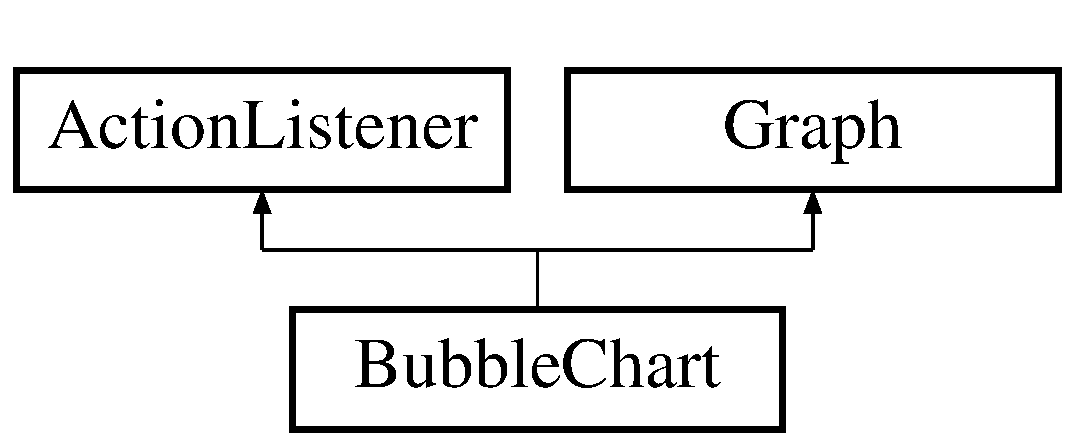
\includegraphics[height=2.000000cm]{class_bubble_chart}
\end{center}
\end{figure}
\subsection*{Public Member Functions}
\begin{DoxyCompactItemize}
\item 
\hyperlink{class_bubble_chart_abde1df172d8b14212f177e1d4c866f7c}{Bubble\-Chart} (String\mbox{[}$\,$\mbox{]}\mbox{[}$\,$\mbox{]} data, \hyperlink{class_dataset}{Dataset} dataset, \hyperlink{class_data_attribute}{Data\-Attribute} setting)
\item 
\hyperlink{class_bubble_chart_afa41fb76ce19f903532f6fef230a4d94}{Bubble\-Chart} (String\mbox{[}$\,$\mbox{]}\mbox{[}$\,$\mbox{]} data, \hyperlink{class_dataset}{Dataset} dataset, \hyperlink{class_data_attribute}{Data\-Attribute} setting, String\mbox{[}$\,$\mbox{]}\mbox{[}$\,$\mbox{]} second\-Data, \hyperlink{class_dataset}{Dataset} second\-Dataset, \hyperlink{class_data_attribute}{Data\-Attribute} second\-Setting)
\item 
\hyperlink{class_bubble_chart_a6c75dda5d1a8e5596652926370ac1e0e}{Bubble\-Chart} (\hyperlink{class_data_attribute}{Data\-Attribute} setting)
\item 
\hyperlink{class_bubble_chart_a4d6417f505cc2bb349d3c3bce02d185d}{Bubble\-Chart} (\hyperlink{class_data_attribute}{Data\-Attribute} setting, \hyperlink{class_data_attribute}{Data\-Attribute} second\-Setting)
\item 
\hyperlink{class_bubble_chart_a90418fabcda19061a4d395f18ee5f48d}{Bubble\-Chart} ()
\item 
void \hyperlink{class_bubble_chart_aa0b9dd81383c38083695c6dbab56fc03}{action\-Performed} (Action\-Event e)
\item 
String \hyperlink{class_bubble_chart_a57559533fd32fd0af64c1196e7278277}{Set\-Label\-X} (String m\-\_\-x\-Label)
\item 
String \hyperlink{class_bubble_chart_a9016f31e007668efd3f8ec384e30c1d9}{Set\-Label\-Y} (String m\-\_\-y\-Label)
\item 
String \hyperlink{class_bubble_chart_a0a4eb8d3bd5c2e13229b290e06dff4c7}{Set\-Title} (String m\-\_\-graph\-Title)
\item 
\hyperlink{class_data_attribute}{Data\-Attribute} \hyperlink{class_bubble_chart_ad4ed746599c2a16959123ca77d7bea58}{Get\-Setting} ()
\item 
X\-Y\-Z\-Dataset \hyperlink{class_bubble_chart_a29cb4d22e401dd9f621501356cd1ebaf}{Create\-Dataset} (String\mbox{[}$\,$\mbox{]}\mbox{[}$\,$\mbox{]} data)
\item 
X\-Y\-Z\-Dataset \hyperlink{class_bubble_chart_a69a32c69ec1225221e9daf6488d284d3}{Create\-Second\-Dataset} (String\mbox{[}$\,$\mbox{]}\mbox{[}$\,$\mbox{]} data)
\end{DoxyCompactItemize}
\subsection*{Static Public Member Functions}
\begin{DoxyCompactItemize}
\item 
static void \hyperlink{class_bubble_chart_a7f8e8bb3079e6dc19d8e88cd03e71c9e}{main} (String\mbox{[}$\,$\mbox{]} args)
\end{DoxyCompactItemize}


\subsection{Detailed Description}
A class that creates a single Bubble \hyperlink{interface_chart}{Chart} or two Bubble \hyperlink{interface_chart}{Chart} visualizations from a 2\-D Array of data \textbackslash{} see \hyperlink{_graph_8java}{Graph.\-java}. 

\begin{DoxyDate}{Date}
30/04/13 
\end{DoxyDate}
\begin{DoxySeeAlso}{See Also}
This class is responsible for making the Bubble chart It was made using J\-Free\-Chart and following examples on how to set up the Bubble chart It uses the \hyperlink{_graph_8java}{Graph.\-java} to return a J\-Free\-Chart 
\end{DoxySeeAlso}


\subsection{Constructor \& Destructor Documentation}
\hypertarget{class_bubble_chart_abde1df172d8b14212f177e1d4c866f7c}{\index{Bubble\-Chart@{Bubble\-Chart}!Bubble\-Chart@{Bubble\-Chart}}
\index{Bubble\-Chart@{Bubble\-Chart}!BubbleChart@{Bubble\-Chart}}
\subsubsection[{Bubble\-Chart}]{\setlength{\rightskip}{0pt plus 5cm}Bubble\-Chart.\-Bubble\-Chart (
\begin{DoxyParamCaption}
\item[{String}]{data\mbox{[}$\,$\mbox{]}\mbox{[}$\,$\mbox{]}, }
\item[{{\bf Dataset}}]{dataset, }
\item[{{\bf Data\-Attribute}}]{setting}
\end{DoxyParamCaption}
)}}\label{class_bubble_chart_abde1df172d8b14212f177e1d4c866f7c}
creates a constructor taking in the following parameters\-:


\begin{DoxyParams}{Parameters}
{\em String\mbox{[}$\,$\mbox{]}\mbox{[}$\,$\mbox{]}} & data -\/ data used to create the visualisation. \\
\hline
{\em \hyperlink{class_dataset}{Dataset}} & dataset -\/ the dataset used (rows and columns) \\
\hline
{\em \hyperlink{class_data_attribute}{Data\-Attribute}} & setting -\/ Data attributes \\
\hline
\end{DoxyParams}

\begin{DoxyCode}
49                                                \{
50         
51         m\_Data = data;
52         m\_Setting = setting;
53         m\_ChartTitle = setting.\hyperlink{class_data_attribute_ade9747a192ba22fe1020e874bff6a48c}{GetTitle}();
54         m\_XLabel = setting.\hyperlink{class_data_attribute_aecb451704a87d77dd80dbad8a19099d1}{GetAxisLabelX}();
55         m\_YLabel = setting.\hyperlink{class_data_attribute_af5f68794cd0195d42135d5e48120ccc0}{GetAxisLabelY}();
56         m\_Col = dataset.\hyperlink{class_dataset_ab922bef50c8aa1531de8704731779246}{GetNoOfCols}();
57         m\_Row = dataset.\hyperlink{class_dataset_a91257a605317576e87e1c32e54739e51}{GetNoOfRows}();
58         m\_C1 = setting.\hyperlink{class_data_attribute_a0f4a54973bc44b0526f78bda945dc81b}{GetSelectedXIndex}();
59         m\_C2 = setting.\hyperlink{class_data_attribute_a82e7519853d9f470ea183dd0c39a03d6}{GetSelectedYIndex}();
60         m\_C3 = setting.\hyperlink{class_data_attribute_a802ca8ea739cff583380ea27647250c7}{GetSelectedZIndex}();
61         
62         m\_XMin = setting.\hyperlink{class_data_attribute_afa9da883abc4abad5f64c045de114c50}{GetXAxisMin}();
63         m\_XMax = setting.\hyperlink{class_data_attribute_a81243eb8f7008e05e74b0f3571d2f08d}{GetYAxisMax}();
64         m\_XScale = setting.\hyperlink{class_data_attribute_a5a1de25600487aa958a19ce01151fea4}{GetXAxisScale}();
65         m\_YScale = setting.\hyperlink{class_data_attribute_a95259727ce91efc0e0eaa28487d944c5}{GetYAxisScale}();
66         
67         \hyperlink{class_bubble_chart_a29cb4d22e401dd9f621501356cd1ebaf}{CreateDataset}( m\_Data );
68         ShowChart( m\_Dataset );
69     \} 
\end{DoxyCode}
\hypertarget{class_bubble_chart_afa41fb76ce19f903532f6fef230a4d94}{\index{Bubble\-Chart@{Bubble\-Chart}!Bubble\-Chart@{Bubble\-Chart}}
\index{Bubble\-Chart@{Bubble\-Chart}!BubbleChart@{Bubble\-Chart}}
\subsubsection[{Bubble\-Chart}]{\setlength{\rightskip}{0pt plus 5cm}Bubble\-Chart.\-Bubble\-Chart (
\begin{DoxyParamCaption}
\item[{String}]{data\mbox{[}$\,$\mbox{]}\mbox{[}$\,$\mbox{]}, }
\item[{{\bf Dataset}}]{dataset, }
\item[{{\bf Data\-Attribute}}]{setting, }
\item[{String}]{second\-Data\mbox{[}$\,$\mbox{]}\mbox{[}$\,$\mbox{]}, }
\item[{{\bf Dataset}}]{second\-Dataset, }
\item[{{\bf Data\-Attribute}}]{second\-Setting}
\end{DoxyParamCaption}
)}}\label{class_bubble_chart_afa41fb76ce19f903532f6fef230a4d94}
creates a constructor taking in the following parameters\-:


\begin{DoxyParams}{Parameters}
{\em String\mbox{[}$\,$\mbox{]}\mbox{[}$\,$\mbox{]}} & data -\/ data used to create the visualisation. \\
\hline
{\em \hyperlink{class_dataset}{Dataset}} & dataset -\/ the dataset used (rows and columns) \\
\hline
{\em \hyperlink{class_data_attribute}{Data\-Attribute}} & setting -\/ Data attributes \\
\hline
{\em String\mbox{[}$\,$\mbox{]}\mbox{[}$\,$\mbox{]}} & second\-Data -\/ second data used to create the visualisation. \\
\hline
{\em \hyperlink{class_dataset}{Dataset}} & second\-Dataset -\/ the second dataset used (rows and columns) \\
\hline
{\em \hyperlink{class_data_attribute}{Data\-Attribute}} & second\-Setting -\/ Second Data attributes \\
\hline
\end{DoxyParams}

\begin{DoxyCode}
83                                           \{
84 
85         m\_Data = data;
86         m\_Setting = setting;
87         m\_ChartTitle = setting.\hyperlink{class_data_attribute_ade9747a192ba22fe1020e874bff6a48c}{GetTitle}();
88         m\_XLabel = setting.\hyperlink{class_data_attribute_aecb451704a87d77dd80dbad8a19099d1}{GetAxisLabelX}();
89         m\_YLabel = setting.\hyperlink{class_data_attribute_af5f68794cd0195d42135d5e48120ccc0}{GetAxisLabelY}();
90         m\_Col = dataset.\hyperlink{class_dataset_ab922bef50c8aa1531de8704731779246}{GetNoOfCols}();
91         m\_Row = dataset.\hyperlink{class_dataset_a91257a605317576e87e1c32e54739e51}{GetNoOfRows}();
92         m\_C1 = setting.\hyperlink{class_data_attribute_a0f4a54973bc44b0526f78bda945dc81b}{GetSelectedXIndex}();
93         m\_C2 = setting.\hyperlink{class_data_attribute_a82e7519853d9f470ea183dd0c39a03d6}{GetSelectedYIndex}();
94         m\_C3 = setting.\hyperlink{class_data_attribute_a802ca8ea739cff583380ea27647250c7}{GetSelectedZIndex}();
95         
96         m\_XMin = setting.\hyperlink{class_data_attribute_afa9da883abc4abad5f64c045de114c50}{GetXAxisMin}();
97         m\_XMax = setting.\hyperlink{class_data_attribute_a81243eb8f7008e05e74b0f3571d2f08d}{GetYAxisMax}();
98         m\_XScale = setting.\hyperlink{class_data_attribute_a5a1de25600487aa958a19ce01151fea4}{GetXAxisScale}();
99         m\_YScale = setting.\hyperlink{class_data_attribute_a95259727ce91efc0e0eaa28487d944c5}{GetYAxisScale}();
100         
101         m\_SecondData = secondData;
102         m\_SecondSetting = secondSetting;
103         m\_SecondChartTitle = secondSetting.\hyperlink{class_data_attribute_a4079522c93025fce7569eaed585f4aeb}{GetSecondTitle}();
104         m\_SecondXLabel = secondSetting.\hyperlink{class_data_attribute_a8ace4cb1fee9e2abeabe3efc9a190c8f}{GetSecondAxisLabelX}();
105         m\_SecondYLabel = secondSetting.\hyperlink{class_data_attribute_a6efb7e067317898feefbbf6bd472b998}{GetSecondAxisLabelY}();
106         m\_SecondCol = secondDataset.\hyperlink{class_dataset_ab922bef50c8aa1531de8704731779246}{GetNoOfCols}();
107         m\_SecondRow = secondDataset.\hyperlink{class_dataset_a91257a605317576e87e1c32e54739e51}{GetNoOfRows}();
108         m\_SecondC1 = secondSetting.\hyperlink{class_data_attribute_a7f501790eee650ddf9ac17c4f63a3995}{GetSecondSelectedXIndex}();
109         m\_SecondC2 = secondSetting.\hyperlink{class_data_attribute_a6f61ad05915f4aa31ad3dba00596da64}{GetSecondSelectedYIndex}();
110         m\_SecondC3 = secondSetting.\hyperlink{class_data_attribute_ab8aad538c86b04b4b9a962b7e07e6bc3}{GetSecondSelectedZIndex}();
111         
112          \hyperlink{class_bubble_chart_a29cb4d22e401dd9f621501356cd1ebaf}{CreateDataset}(m\_Data);
113          \hyperlink{class_bubble_chart_a69a32c69ec1225221e9daf6488d284d3}{CreateSecondDataset}(m\_SecondData);
114          ShowChart(m\_Dataset, m\_SecondDataset);
115     \} 
\end{DoxyCode}
\hypertarget{class_bubble_chart_a6c75dda5d1a8e5596652926370ac1e0e}{\index{Bubble\-Chart@{Bubble\-Chart}!Bubble\-Chart@{Bubble\-Chart}}
\index{Bubble\-Chart@{Bubble\-Chart}!BubbleChart@{Bubble\-Chart}}
\subsubsection[{Bubble\-Chart}]{\setlength{\rightskip}{0pt plus 5cm}Bubble\-Chart.\-Bubble\-Chart (
\begin{DoxyParamCaption}
\item[{{\bf Data\-Attribute}}]{setting}
\end{DoxyParamCaption}
)}}\label{class_bubble_chart_a6c75dda5d1a8e5596652926370ac1e0e}
constructor for J\-Unit Tests 
\begin{DoxyParams}{Parameters}
{\em setting} & \\
\hline
\end{DoxyParams}

\begin{DoxyCode}
121                                               \{
122         m\_ChartTitle = setting.\hyperlink{class_data_attribute_ade9747a192ba22fe1020e874bff6a48c}{GetTitle}();
123         m\_Setting = setting;
124         m\_XLabel = setting.\hyperlink{class_data_attribute_aecb451704a87d77dd80dbad8a19099d1}{GetAxisLabelX}();
125         m\_YLabel = setting.\hyperlink{class_data_attribute_af5f68794cd0195d42135d5e48120ccc0}{GetAxisLabelY}();
126         m\_C1 = setting.\hyperlink{class_data_attribute_a0f4a54973bc44b0526f78bda945dc81b}{GetSelectedXIndex}();
127         m\_C2 = setting.\hyperlink{class_data_attribute_a82e7519853d9f470ea183dd0c39a03d6}{GetSelectedYIndex}();
128         m\_XMin = setting.\hyperlink{class_data_attribute_afa9da883abc4abad5f64c045de114c50}{GetXAxisMin}();
129         m\_XMax = setting.\hyperlink{class_data_attribute_ada370712422c7cbd21b7be4a0d88caf7}{GetXAxisMax}();
130         m\_YMin = setting.\hyperlink{class_data_attribute_af0786b4de674874c0bb8ca9dbe1519c6}{GetYAxisMin}();
131         m\_YMax = setting.\hyperlink{class_data_attribute_a81243eb8f7008e05e74b0f3571d2f08d}{GetYAxisMax}();
132         m\_XScale = setting.\hyperlink{class_data_attribute_a5a1de25600487aa958a19ce01151fea4}{GetXAxisScale}();
133         m\_YScale = setting.\hyperlink{class_data_attribute_a95259727ce91efc0e0eaa28487d944c5}{GetYAxisScale}();
134     \}
\end{DoxyCode}
\hypertarget{class_bubble_chart_a4d6417f505cc2bb349d3c3bce02d185d}{\index{Bubble\-Chart@{Bubble\-Chart}!Bubble\-Chart@{Bubble\-Chart}}
\index{Bubble\-Chart@{Bubble\-Chart}!BubbleChart@{Bubble\-Chart}}
\subsubsection[{Bubble\-Chart}]{\setlength{\rightskip}{0pt plus 5cm}Bubble\-Chart.\-Bubble\-Chart (
\begin{DoxyParamCaption}
\item[{{\bf Data\-Attribute}}]{setting, }
\item[{{\bf Data\-Attribute}}]{second\-Setting}
\end{DoxyParamCaption}
)}}\label{class_bubble_chart_a4d6417f505cc2bb349d3c3bce02d185d}
second constructor for J\-Unit Tests 
\begin{DoxyParams}{Parameters}
{\em setting} & \\
\hline
{\em second\-Setting} & \\
\hline
\end{DoxyParams}

\begin{DoxyCode}
140                                                                            \{
141         m\_ChartTitle = setting.\hyperlink{class_data_attribute_ade9747a192ba22fe1020e874bff6a48c}{GetTitle}();
142         m\_Setting = setting;
143         m\_XLabel = setting.\hyperlink{class_data_attribute_aecb451704a87d77dd80dbad8a19099d1}{GetAxisLabelX}();
144         m\_YLabel = setting.\hyperlink{class_data_attribute_af5f68794cd0195d42135d5e48120ccc0}{GetAxisLabelY}();
145         m\_C1 = setting.\hyperlink{class_data_attribute_a0f4a54973bc44b0526f78bda945dc81b}{GetSelectedXIndex}();
146         m\_C2 = setting.\hyperlink{class_data_attribute_a82e7519853d9f470ea183dd0c39a03d6}{GetSelectedYIndex}();
147         m\_XMin = setting.\hyperlink{class_data_attribute_afa9da883abc4abad5f64c045de114c50}{GetXAxisMin}();
148         m\_XMax = setting.\hyperlink{class_data_attribute_ada370712422c7cbd21b7be4a0d88caf7}{GetXAxisMax}();
149         m\_YMin = setting.\hyperlink{class_data_attribute_af0786b4de674874c0bb8ca9dbe1519c6}{GetYAxisMin}();
150         m\_YMax = setting.\hyperlink{class_data_attribute_a81243eb8f7008e05e74b0f3571d2f08d}{GetYAxisMax}();
151         m\_XScale = setting.\hyperlink{class_data_attribute_a5a1de25600487aa958a19ce01151fea4}{GetXAxisScale}();
152         m\_YScale = setting.\hyperlink{class_data_attribute_a95259727ce91efc0e0eaa28487d944c5}{GetYAxisScale}();
153         
154         m\_SecondChartTitle = secondSetting.\hyperlink{class_data_attribute_a4079522c93025fce7569eaed585f4aeb}{GetSecondTitle}();
155         m\_SecondSetting = secondSetting;
156         m\_SecondXLabel = secondSetting.\hyperlink{class_data_attribute_a8ace4cb1fee9e2abeabe3efc9a190c8f}{GetSecondAxisLabelX}();
157         m\_SecondYLabel = secondSetting.\hyperlink{class_data_attribute_a6efb7e067317898feefbbf6bd472b998}{GetSecondAxisLabelY}();
158         m\_SecondC1 = secondSetting.\hyperlink{class_data_attribute_a7f501790eee650ddf9ac17c4f63a3995}{GetSecondSelectedXIndex}();
159         m\_SecondC2 = secondSetting.\hyperlink{class_data_attribute_a6f61ad05915f4aa31ad3dba00596da64}{GetSecondSelectedYIndex}();
160     \}
\end{DoxyCode}
\hypertarget{class_bubble_chart_a90418fabcda19061a4d395f18ee5f48d}{\index{Bubble\-Chart@{Bubble\-Chart}!Bubble\-Chart@{Bubble\-Chart}}
\index{Bubble\-Chart@{Bubble\-Chart}!BubbleChart@{Bubble\-Chart}}
\subsubsection[{Bubble\-Chart}]{\setlength{\rightskip}{0pt plus 5cm}Bubble\-Chart.\-Bubble\-Chart (
\begin{DoxyParamCaption}
{}
\end{DoxyParamCaption}
)}}\label{class_bubble_chart_a90418fabcda19061a4d395f18ee5f48d}
second empty constructor for J\-Unit Tests 
\begin{DoxyCode}
165 \{\}
\end{DoxyCode}


\subsection{Member Function Documentation}
\hypertarget{class_bubble_chart_aa0b9dd81383c38083695c6dbab56fc03}{\index{Bubble\-Chart@{Bubble\-Chart}!action\-Performed@{action\-Performed}}
\index{action\-Performed@{action\-Performed}!BubbleChart@{Bubble\-Chart}}
\subsubsection[{action\-Performed}]{\setlength{\rightskip}{0pt plus 5cm}void Bubble\-Chart.\-action\-Performed (
\begin{DoxyParamCaption}
\item[{Action\-Event}]{e}
\end{DoxyParamCaption}
)}}\label{class_bubble_chart_aa0b9dd81383c38083695c6dbab56fc03}
allows user to select the colour of the points on the Bubble chart 
\begin{DoxyCode}
170                                                  \{
171         \textcolor{keywordflow}{if}( e.getSource() == m\_ColChangeButton ) \{
172             \hyperlink{class_colour_map}{ColourMap} cM = \textcolor{keyword}{new} \hyperlink{class_colour_map}{ColourMap}();
173             cM.\hyperlink{class_colour_map_a9f696ea699b7fc471bb2dde6f1d1ce09}{SetupData}( m\_Plot.getSeriesCount(), 
174                           m\_Renderer );
175             cM.setVisible( \textcolor{keyword}{false} );
176         \}
177     \}
\end{DoxyCode}
\hypertarget{class_bubble_chart_a29cb4d22e401dd9f621501356cd1ebaf}{\index{Bubble\-Chart@{Bubble\-Chart}!Create\-Dataset@{Create\-Dataset}}
\index{Create\-Dataset@{Create\-Dataset}!BubbleChart@{Bubble\-Chart}}
\subsubsection[{Create\-Dataset}]{\setlength{\rightskip}{0pt plus 5cm}X\-Y\-Z\-Dataset Bubble\-Chart.\-Create\-Dataset (
\begin{DoxyParamCaption}
\item[{String}]{data\mbox{[}$\,$\mbox{]}\mbox{[}$\,$\mbox{]}}
\end{DoxyParamCaption}
)}}\label{class_bubble_chart_a29cb4d22e401dd9f621501356cd1ebaf}
Method creates the X\-Y\-Z \hyperlink{class_dataset}{Dataset} needed for the visualisation 
\begin{DoxyParams}{Parameters}
{\em data} & \\
\hline
\end{DoxyParams}
\begin{DoxyReturn}{Returns}
dataset 
\end{DoxyReturn}

\begin{DoxyCode}
222                                                      \{
223         m\_Dataset = \textcolor{keyword}{new} DefaultXYZDataset();
224         \textcolor{keywordflow}{for}(\textcolor{keywordtype}{int} r = 0; r < m\_Row;r++) \{
225             \textcolor{keywordtype}{double} xArray[] = \textcolor{keyword}{new} \textcolor{keywordtype}{double}[m\_Row];
226             \textcolor{keywordtype}{double} yArray[] = \textcolor{keyword}{new} \textcolor{keywordtype}{double}[m\_Row];
227             \textcolor{keywordtype}{double} zArray[] = \textcolor{keyword}{new} \textcolor{keywordtype}{double}[m\_Row];
228             
229             xArray[r] = Double.parseDouble(data[m\_C1][r]);
230             yArray[r] = Double.parseDouble(data[m\_C2][r]);
231             zArray[r] = Double.parseDouble(data[m\_C3][r]);
232             
233             \textcolor{keywordtype}{double} ad3[][] = \{
234                     xArray, yArray, zArray
235             \};
236             m\_Dataset.addSeries(\textcolor{stringliteral}{"Series "} + r, ad3);
237         \}
238         \textcolor{keywordflow}{return} m\_Dataset;
239     \}
\end{DoxyCode}
\hypertarget{class_bubble_chart_a69a32c69ec1225221e9daf6488d284d3}{\index{Bubble\-Chart@{Bubble\-Chart}!Create\-Second\-Dataset@{Create\-Second\-Dataset}}
\index{Create\-Second\-Dataset@{Create\-Second\-Dataset}!BubbleChart@{Bubble\-Chart}}
\subsubsection[{Create\-Second\-Dataset}]{\setlength{\rightskip}{0pt plus 5cm}X\-Y\-Z\-Dataset Bubble\-Chart.\-Create\-Second\-Dataset (
\begin{DoxyParamCaption}
\item[{String}]{data\mbox{[}$\,$\mbox{]}\mbox{[}$\,$\mbox{]}}
\end{DoxyParamCaption}
)}}\label{class_bubble_chart_a69a32c69ec1225221e9daf6488d284d3}
Method creates the second X\-Y\-Z \hyperlink{class_dataset}{Dataset} needed for the visualisation 
\begin{DoxyParams}{Parameters}
{\em data} & \\
\hline
\end{DoxyParams}
\begin{DoxyReturn}{Returns}
dataset 
\end{DoxyReturn}

\begin{DoxyCode}
245                                                            \{    
246         m\_SecondDataset = \textcolor{keyword}{new} DefaultXYZDataset();
247         \textcolor{keywordflow}{for}(\textcolor{keywordtype}{int} r = 0; r < m\_SecondRow;r++) \{
248             \textcolor{keywordtype}{double} xArray[] = \textcolor{keyword}{new} \textcolor{keywordtype}{double}[m\_SecondRow];
249             \textcolor{keywordtype}{double} yArray[] = \textcolor{keyword}{new} \textcolor{keywordtype}{double}[m\_SecondRow];
250             \textcolor{keywordtype}{double} zArray[] = \textcolor{keyword}{new} \textcolor{keywordtype}{double}[m\_SecondRow];
251             
252             xArray[r] = Double.parseDouble(data[m\_SecondC1][r]);
253             yArray[r] = Double.parseDouble(data[m\_SecondC2][r]);
254             zArray[r] = Double.parseDouble(data[m\_SecondC3][r]);
255             
256             \textcolor{keywordtype}{double} ad3[][] = \{
257                     xArray, yArray, zArray
258             \};
259             m\_SecondDataset.addSeries(\textcolor{stringliteral}{"Series "} + r, ad3);
260         \}
261         \textcolor{keywordflow}{return} m\_SecondDataset;
262     \}
\end{DoxyCode}
\hypertarget{class_bubble_chart_ad4ed746599c2a16959123ca77d7bea58}{\index{Bubble\-Chart@{Bubble\-Chart}!Get\-Setting@{Get\-Setting}}
\index{Get\-Setting@{Get\-Setting}!BubbleChart@{Bubble\-Chart}}
\subsubsection[{Get\-Setting}]{\setlength{\rightskip}{0pt plus 5cm}{\bf Data\-Attribute} Bubble\-Chart.\-Get\-Setting (
\begin{DoxyParamCaption}
{}
\end{DoxyParamCaption}
)}}\label{class_bubble_chart_ad4ed746599c2a16959123ca77d7bea58}
Gets the settings \begin{DoxyReturn}{Returns}
\hyperlink{class_data_attribute}{Data\-Attribute} setting 
\end{DoxyReturn}

\begin{DoxyCode}
213                                       \{
214         \textcolor{keywordflow}{return} m\_Setting;
215     \}
\end{DoxyCode}
\hypertarget{class_bubble_chart_a7f8e8bb3079e6dc19d8e88cd03e71c9e}{\index{Bubble\-Chart@{Bubble\-Chart}!main@{main}}
\index{main@{main}!BubbleChart@{Bubble\-Chart}}
\subsubsection[{main}]{\setlength{\rightskip}{0pt plus 5cm}static void Bubble\-Chart.\-main (
\begin{DoxyParamCaption}
\item[{String\mbox{[}$\,$\mbox{]}}]{args}
\end{DoxyParamCaption}
)\hspace{0.3cm}{\ttfamily [static]}}}\label{class_bubble_chart_a7f8e8bb3079e6dc19d8e88cd03e71c9e}
main method to carry out J\-Unit Tests 
\begin{DoxyCode}
397                                              \{
398     
399         \hyperlink{class_data_attribute}{DataAttribute} test = \hyperlink{class_data_attribute}{DataAttribute}.
      \hyperlink{class_data_attribute_a9c7a1923698c1530fa38c959596199bc}{GetTestDataAttribute}();
400         \hyperlink{class_bubble_chart}{BubbleChart} bubbleTest = \textcolor{keyword}{new} \hyperlink{class_bubble_chart_a90418fabcda19061a4d395f18ee5f48d}{BubbleChart}(test);
401         \hyperlink{class_data_attribute}{DataAttribute} secondTest = \hyperlink{class_data_attribute}{DataAttribute}.
      \hyperlink{class_data_attribute_a9c7a1923698c1530fa38c959596199bc}{GetTestDataAttribute}();
402         \hyperlink{class_bubble_chart}{BubbleChart} secondBubbleTest = \textcolor{keyword}{new} \hyperlink{class_bubble_chart_a90418fabcda19061a4d395f18ee5f48d}{BubbleChart}(secondTest);
403         
404         Random gen = \textcolor{keyword}{new} Random();
405         
406         \textcolor{keywordtype}{double} x1 = gen.nextDouble() * VALUE\_MULTIPLY + VALUE\_ADD;
407         \textcolor{keywordtype}{double} x2 = gen.nextDouble() * VALUE\_MULTIPLY + VALUE\_ADD;
408         \textcolor{keywordtype}{double} x3 = gen.nextDouble() * VALUE\_MULTIPLY + VALUE\_ADD;
409         \textcolor{keywordtype}{double}[] xTest = \{x1, x2, x3\};      
410         
411         \textcolor{keywordtype}{double} y1 = gen.nextDouble() * VALUE\_MULTIPLY + VALUE\_ADD + VALUE\_ADD;
412         \textcolor{keywordtype}{double} y2 = gen.nextDouble() * VALUE\_MULTIPLY + VALUE\_ADD + VALUE\_ADD;
413         \textcolor{keywordtype}{double} y3 = gen.nextDouble() * VALUE\_MULTIPLY + VALUE\_ADD + VALUE\_ADD;
414         \textcolor{keywordtype}{double}[] yTest = \{y1, y2, y3\};
415         
416         \textcolor{keywordtype}{double} z1 = gen.nextDouble() * VALUE\_MULTIPLY + VALUE\_ADD + VALUE\_ADD;
417         \textcolor{keywordtype}{double} z2 = gen.nextDouble() * VALUE\_MULTIPLY + VALUE\_ADD + VALUE\_ADD;
418         \textcolor{keywordtype}{double} z3 = gen.nextDouble() * VALUE\_MULTIPLY + VALUE\_ADD + VALUE\_ADD;
419         \textcolor{keywordtype}{double}[] zTest = \{z1, z2, z3\};
420         
421         \textcolor{keywordtype}{double}[][] xyzTest = \{xTest, yTest, zTest\};
422         \textcolor{keywordtype}{double}[][] xyzSecondTest = \{xTest, yTest, zTest\};
423         
424         DefaultXYZDataset dataset = \textcolor{keyword}{new} DefaultXYZDataset();
425         dataset.addSeries(\textcolor{stringliteral}{"testSeries"}, xyzTest);
426         bubbleTest.\hyperlink{class_bubble_chart_ad4ed746599c2a16959123ca77d7bea58}{GetSetting}().\hyperlink{class_data_attribute_a46b8473768d9ba3609e5f5994e903a7c}{SetUseDefault}(\textcolor{keyword}{false});
427         bubbleTest.\hyperlink{class_bubble_chart_ad4ed746599c2a16959123ca77d7bea58}{GetSetting}().\hyperlink{class_data_attribute_acd1994e216d21da1f3e7ea2819145fe9}{SetXAxisMin}(MIN);
428         bubbleTest.\hyperlink{class_bubble_chart_ad4ed746599c2a16959123ca77d7bea58}{GetSetting}().\hyperlink{class_data_attribute_a6aedbe05a82f23d6abca00f8b85bf1ff}{SetXAxisMax}(MAX);
429         bubbleTest.\hyperlink{class_bubble_chart_ad4ed746599c2a16959123ca77d7bea58}{GetSetting}().\hyperlink{class_data_attribute_afacd93a87dbe8ed03d4dc9a50e44851f}{SetYAxisMin}(MIN);
430         bubbleTest.\hyperlink{class_bubble_chart_ad4ed746599c2a16959123ca77d7bea58}{GetSetting}().\hyperlink{class_data_attribute_a6aedbe05a82f23d6abca00f8b85bf1ff}{SetXAxisMax}(MAX);
431         
432         
433         secondBubbleTest.ShowChart(dataset);
434         
435         DefaultXYZDataset secondDataset = \textcolor{keyword}{new} DefaultXYZDataset();
436         secondDataset.addSeries(\textcolor{stringliteral}{"SecondTestSeries"}, xyzSecondTest);
437         
438         secondBubbleTest.\hyperlink{class_bubble_chart_ad4ed746599c2a16959123ca77d7bea58}{GetSetting}().\hyperlink{class_data_attribute_a46b8473768d9ba3609e5f5994e903a7c}{SetUseDefault}(\textcolor{keyword}{false});
439         secondBubbleTest.\hyperlink{class_bubble_chart_ad4ed746599c2a16959123ca77d7bea58}{GetSetting}().\hyperlink{class_data_attribute_acd1994e216d21da1f3e7ea2819145fe9}{SetXAxisMin}(MIN);
440         secondBubbleTest.\hyperlink{class_bubble_chart_ad4ed746599c2a16959123ca77d7bea58}{GetSetting}().\hyperlink{class_data_attribute_a6aedbe05a82f23d6abca00f8b85bf1ff}{SetXAxisMax}(MAX);
441         secondBubbleTest.\hyperlink{class_bubble_chart_ad4ed746599c2a16959123ca77d7bea58}{GetSetting}().\hyperlink{class_data_attribute_afacd93a87dbe8ed03d4dc9a50e44851f}{SetYAxisMin}(MIN);
442         secondBubbleTest.\hyperlink{class_bubble_chart_ad4ed746599c2a16959123ca77d7bea58}{GetSetting}().\hyperlink{class_data_attribute_a6aedbe05a82f23d6abca00f8b85bf1ff}{SetXAxisMax}(MAX);
443         
444         bubbleTest.ShowChart(dataset, secondDataset);
445         
446     \}
\end{DoxyCode}
\hypertarget{class_bubble_chart_a57559533fd32fd0af64c1196e7278277}{\index{Bubble\-Chart@{Bubble\-Chart}!Set\-Label\-X@{Set\-Label\-X}}
\index{Set\-Label\-X@{Set\-Label\-X}!BubbleChart@{Bubble\-Chart}}
\subsubsection[{Set\-Label\-X}]{\setlength{\rightskip}{0pt plus 5cm}String Bubble\-Chart.\-Set\-Label\-X (
\begin{DoxyParamCaption}
\item[{String}]{m\-\_\-x\-Label}
\end{DoxyParamCaption}
)}}\label{class_bubble_chart_a57559533fd32fd0af64c1196e7278277}

\begin{DoxyParams}{Parameters}
{\em m\-\_\-x\-Label} & -\/ the x axis label passed from users to the graph \\
\hline
\end{DoxyParams}
\begin{DoxyReturn}{Returns}
m\-\_\-label\-X -\/ returns the user's x label value 
\end{DoxyReturn}

\begin{DoxyCode}
184                                                \{
185         String m\_labelX = m\_xLabel;
186         \textcolor{keywordflow}{return} m\_labelX;
187     \}
\end{DoxyCode}
\hypertarget{class_bubble_chart_a9016f31e007668efd3f8ec384e30c1d9}{\index{Bubble\-Chart@{Bubble\-Chart}!Set\-Label\-Y@{Set\-Label\-Y}}
\index{Set\-Label\-Y@{Set\-Label\-Y}!BubbleChart@{Bubble\-Chart}}
\subsubsection[{Set\-Label\-Y}]{\setlength{\rightskip}{0pt plus 5cm}String Bubble\-Chart.\-Set\-Label\-Y (
\begin{DoxyParamCaption}
\item[{String}]{m\-\_\-y\-Label}
\end{DoxyParamCaption}
)}}\label{class_bubble_chart_a9016f31e007668efd3f8ec384e30c1d9}

\begin{DoxyParams}{Parameters}
{\em m\-\_\-y\-Label} & -\/ the y axis label passed from users to the graph \\
\hline
\end{DoxyParams}
\begin{DoxyReturn}{Returns}
m\-\_\-label\-Y -\/ returns the user's y label value 
\end{DoxyReturn}

\begin{DoxyCode}
194                                                \{
195         String m\_labelY = m\_yLabel;
196         \textcolor{keywordflow}{return} m\_labelY;
197     \}
\end{DoxyCode}
\hypertarget{class_bubble_chart_a0a4eb8d3bd5c2e13229b290e06dff4c7}{\index{Bubble\-Chart@{Bubble\-Chart}!Set\-Title@{Set\-Title}}
\index{Set\-Title@{Set\-Title}!BubbleChart@{Bubble\-Chart}}
\subsubsection[{Set\-Title}]{\setlength{\rightskip}{0pt plus 5cm}String Bubble\-Chart.\-Set\-Title (
\begin{DoxyParamCaption}
\item[{String}]{m\-\_\-graph\-Title}
\end{DoxyParamCaption}
)}}\label{class_bubble_chart_a0a4eb8d3bd5c2e13229b290e06dff4c7}

\begin{DoxyParams}{Parameters}
{\em m\-\_\-graph\-Title} & -\/ the title passed from users to the graph \\
\hline
\end{DoxyParams}
\begin{DoxyReturn}{Returns}
m\-\_\-label\-Y -\/ returns the user's title value 
\end{DoxyReturn}

\begin{DoxyCode}
204                                                   \{
205         String m\_title = m\_graphTitle;
206         \textcolor{keywordflow}{return} m\_title;
207     \} 
\end{DoxyCode}


The documentation for this class was generated from the following file\-:\begin{DoxyCompactItemize}
\item 
\hyperlink{_bubble_chart_8java}{Bubble\-Chart.\-java}\end{DoxyCompactItemize}

\hypertarget{interface_chart}{\section{Chart Class Reference}
\label{interface_chart}\index{Chart@{Chart}}
}


An interface for all chart classes.  


Inheritance diagram for Chart\-:\begin{figure}[H]
\begin{center}
\leavevmode
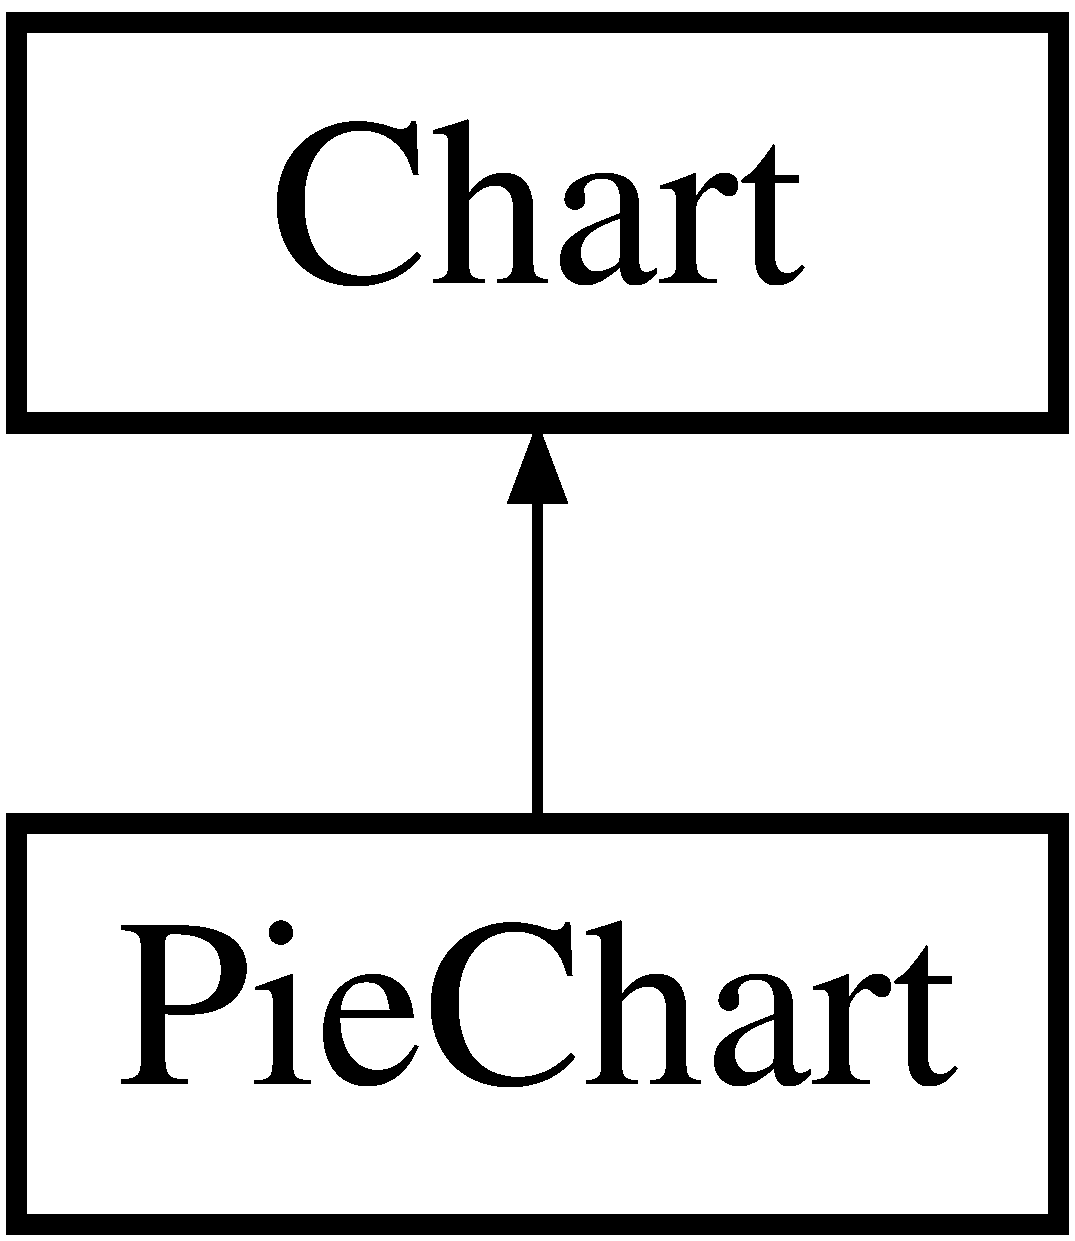
\includegraphics[height=2.000000cm]{interface_chart}
\end{center}
\end{figure}
\subsection*{Public Member Functions}
\begin{DoxyCompactItemize}
\item 
String \hyperlink{interface_chart_a1d38056bfcea7475910c006a90956daa}{Set\-Label\-X} (String x\-Label)
\item 
String \hyperlink{interface_chart_a3b85fe2e2d4f84e2d1b8a472a1967170}{Set\-Title} (String chart\-Title)
\end{DoxyCompactItemize}


\subsection{Detailed Description}
An interface for all chart classes. 

\begin{DoxyDate}{Date}
27/02/13 
\end{DoxyDate}
\begin{DoxySeeAlso}{See Also}
\hyperlink{_column_chart_8java}{Column\-Chart.\-java} 
\end{DoxySeeAlso}


\subsection{Member Function Documentation}
\hypertarget{interface_chart_a1d38056bfcea7475910c006a90956daa}{\index{Chart@{Chart}!Set\-Label\-X@{Set\-Label\-X}}
\index{Set\-Label\-X@{Set\-Label\-X}!Chart@{Chart}}
\subsubsection[{Set\-Label\-X}]{\setlength{\rightskip}{0pt plus 5cm}String Chart.\-Set\-Label\-X (
\begin{DoxyParamCaption}
\item[{String}]{x\-Label}
\end{DoxyParamCaption}
)}}\label{interface_chart_a1d38056bfcea7475910c006a90956daa}
any class that implements \hyperlink{interface_chart}{Chart} is forced to use the x\-Label variable


\begin{DoxyParams}{Parameters}
{\em x\-Label} & the x axis label passed to the chart by the user \\
\hline
\end{DoxyParams}
\hypertarget{interface_chart_a3b85fe2e2d4f84e2d1b8a472a1967170}{\index{Chart@{Chart}!Set\-Title@{Set\-Title}}
\index{Set\-Title@{Set\-Title}!Chart@{Chart}}
\subsubsection[{Set\-Title}]{\setlength{\rightskip}{0pt plus 5cm}String Chart.\-Set\-Title (
\begin{DoxyParamCaption}
\item[{String}]{chart\-Title}
\end{DoxyParamCaption}
)}}\label{interface_chart_a3b85fe2e2d4f84e2d1b8a472a1967170}
any class that implements \hyperlink{interface_chart}{Chart} is forced to use the chart\-Title variable


\begin{DoxyParams}{Parameters}
{\em chart\-Title} & the title passed to the chart by the user \\
\hline
\end{DoxyParams}


The documentation for this class was generated from the following file\-:\begin{DoxyCompactItemize}
\item 
\hyperlink{_chart_8java}{Chart.\-java}\end{DoxyCompactItemize}

\hypertarget{class_colour}{\section{Colour Class Reference}
\label{class_colour}\index{Colour@{Colour}}
}


This class provides user with a choice of some colours to be applied on objects from different graphs/charts/diagrams.  


Inheritance diagram for Colour\-:\begin{figure}[H]
\begin{center}
\leavevmode
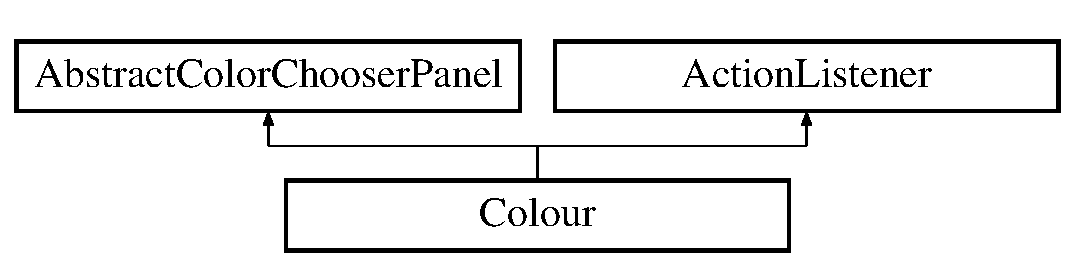
\includegraphics[height=2.000000cm]{class_colour}
\end{center}
\end{figure}
\subsection*{Public Member Functions}
\begin{DoxyCompactItemize}
\item 
\hyperlink{class_colour_a1f07651942561c6818bb26268a39609b}{Colour} ()
\item 
void \hyperlink{class_colour_abc6cd2a5aad847b118f72892e6b39d5a}{update\-Chooser} ()
\item 
void \hyperlink{class_colour_af61690b6ec8f119d9a5f8fc929300b77}{action\-Performed} (Action\-Event e)
\item 
String \hyperlink{class_colour_a1f719e93335cc06a8f5c24fbd50d85a4}{get\-Display\-Name} ()
\item 
Icon \hyperlink{class_colour_afdc3b34af634f3aa1b88bc080c326787}{get\-Small\-Display\-Icon} ()
\item 
Icon \hyperlink{class_colour_a55831e12aaf4110b926ea0240a4fa96f}{get\-Large\-Display\-Icon} ()
\end{DoxyCompactItemize}
\subsection*{Protected Member Functions}
\begin{DoxyCompactItemize}
\item 
void \hyperlink{class_colour_ade22fa4720bb0fc4d477d21fa4785b8c}{build\-Chooser} ()
\end{DoxyCompactItemize}


\subsection{Detailed Description}
This class provides user with a choice of some colours to be applied on objects from different graphs/charts/diagrams. 

\begin{DoxyDate}{Date}
-\/10 February 2013 
\end{DoxyDate}


\subsection{Constructor \& Destructor Documentation}
\hypertarget{class_colour_a1f07651942561c6818bb26268a39609b}{\index{Colour@{Colour}!Colour@{Colour}}
\index{Colour@{Colour}!Colour@{Colour}}
\subsubsection[{Colour}]{\setlength{\rightskip}{0pt plus 5cm}Colour.\-Colour (
\begin{DoxyParamCaption}
{}
\end{DoxyParamCaption}
)}}\label{class_colour_a1f07651942561c6818bb26268a39609b}

\begin{DoxyCode}
19                      \{
20         
21     \}
\end{DoxyCode}


\subsection{Member Function Documentation}
\hypertarget{class_colour_af61690b6ec8f119d9a5f8fc929300b77}{\index{Colour@{Colour}!action\-Performed@{action\-Performed}}
\index{action\-Performed@{action\-Performed}!Colour@{Colour}}
\subsubsection[{action\-Performed}]{\setlength{\rightskip}{0pt plus 5cm}void Colour.\-action\-Performed (
\begin{DoxyParamCaption}
\item[{Action\-Event}]{e}
\end{DoxyParamCaption}
)}}\label{class_colour_af61690b6ec8f119d9a5f8fc929300b77}

\begin{DoxyCode}
161                                                  \{
162         Color newColor = null;
163         String command = ( ( JButton )e.getSource( ) ).getActionCommand( );
164         
165         \textcolor{comment}{/* Switch assigns a new colour, depending on what string "command"
}
166 \textcolor{comment}{         * ( which contains the name of the colour ) contains. 
}
167 \textcolor{comment}{         */}       
168         \textcolor{keywordflow}{switch} ( command ) \{
169             \textcolor{keywordflow}{case} \textcolor{stringliteral}{"green"}:
170                 newColor = Color.GREEN;
171                 \textcolor{keywordflow}{break};
172             \textcolor{keywordflow}{case} \textcolor{stringliteral}{"red"}:
173                 newColor = Color.RED;
174                 \textcolor{keywordflow}{break};
175             \textcolor{keywordflow}{case} \textcolor{stringliteral}{"yellow"}:
176                 newColor = Color.YELLOW;
177                 \textcolor{keywordflow}{break};
178             \textcolor{keywordflow}{case} \textcolor{stringliteral}{"blue"}:
179                 newColor = Color.BLUE;
180                 \textcolor{keywordflow}{break};
181             \textcolor{keywordflow}{case} \textcolor{stringliteral}{"black"}:
182                 newColor = Color.BLACK;
183                 \textcolor{keywordflow}{break};
184             \textcolor{keywordflow}{case} \textcolor{stringliteral}{"cyan"}:
185                 newColor = Color.CYAN;
186                 \textcolor{keywordflow}{break};
187             \textcolor{keywordflow}{case} \textcolor{stringliteral}{"gray"}:
188                 newColor = Color.GRAY;
189                 \textcolor{keywordflow}{break};
190             \textcolor{keywordflow}{case} \textcolor{stringliteral}{"magenta"}:
191                 newColor = Color.MAGENTA;
192                 \textcolor{keywordflow}{break};
193             \textcolor{keywordflow}{case} \textcolor{stringliteral}{"orange"}:
194                 newColor = Color.ORANGE;
195                 \textcolor{keywordflow}{break};
196             \textcolor{keywordflow}{case} \textcolor{stringliteral}{"pink"}:
197                 newColor = Color.PINK;
198                 \textcolor{keywordflow}{break};
199             \textcolor{keywordflow}{case} \textcolor{stringliteral}{"white"}:
200                 newColor = Color.WHITE;
201                 \textcolor{keywordflow}{break};
202             \textcolor{keywordflow}{case} \textcolor{stringliteral}{"lGray"}:
203                 newColor = Color.LIGHT\_GRAY;
204                 \textcolor{keywordflow}{break};
205         \}
206         
207         \textcolor{comment}{/* Changes the colour of the object to the new colour. */}
208         getColorSelectionModel( ).setSelectedColor( newColor );
209     \}
\end{DoxyCode}
\hypertarget{class_colour_ade22fa4720bb0fc4d477d21fa4785b8c}{\index{Colour@{Colour}!build\-Chooser@{build\-Chooser}}
\index{build\-Chooser@{build\-Chooser}!Colour@{Colour}}
\subsubsection[{build\-Chooser}]{\setlength{\rightskip}{0pt plus 5cm}void Colour.\-build\-Chooser (
\begin{DoxyParamCaption}
{}
\end{DoxyParamCaption}
)\hspace{0.3cm}{\ttfamily [protected]}}}\label{class_colour_ade22fa4720bb0fc4d477d21fa4785b8c}

\begin{DoxyCode}
46                                    \{
47         \textcolor{comment}{/* Colour Buttons Group Row Count */}
48         \textcolor{keyword}{final} \textcolor{keywordtype}{int} CBG\_ROW\_COUNT = 3;
49         \textcolor{comment}{/* Colour Button Group Column Count */}
50         \textcolor{keyword}{final} \textcolor{keywordtype}{int} CBG\_COLUMN\_COUNT = 4;
51         \textcolor{comment}{/* Colour Button Height */}
52         \textcolor{keyword}{final} \textcolor{keywordtype}{int} CB\_HEIGHT = 20;
53         \textcolor{comment}{/* Colour Button Width */}
54         \textcolor{keyword}{final} \textcolor{keywordtype}{int} CB\_WIDTH = 20;
55         
56         setLayout( \textcolor{keyword}{new} GridLayout( CBG\_ROW\_COUNT, CBG\_COLUMN\_COUNT ) );
57         \textcolor{comment}{/* Groups default colours into specific row and column count */}
58         
59         ButtonGroup colourButtons = \textcolor{keyword}{new} ButtonGroup( );
60         colourButtons.getButtonCount( );
61         
62         \textcolor{comment}{/* White Colour Button */}
63         whiteButton = createColour(\textcolor{stringliteral}{"white"});
64         whiteButton.setBackground(Color.WHITE);
65         whiteButton.setPreferredSize(\textcolor{keyword}{new} Dimension(CB\_WIDTH, CB\_HEIGHT));
66         whiteButton.setOpaque(\textcolor{keyword}{true});
67         colourButtons.add(whiteButton);
68         add(whiteButton);
69         
70         \textcolor{comment}{/* Light Gray Colour Button */}
71         lGrayButton = createColour(\textcolor{stringliteral}{"lGray"});
72         lGrayButton.setBackground(Color.LIGHT\_GRAY);
73         lGrayButton.setPreferredSize(\textcolor{keyword}{new} Dimension(CB\_WIDTH, CB\_HEIGHT));
74         lGrayButton.setOpaque(\textcolor{keyword}{true});
75         colourButtons.add(lGrayButton);
76         add(lGrayButton);
77         
78         \textcolor{comment}{/* Gray Colour Button */}
79         grayButton = createColour(\textcolor{stringliteral}{"gray"});
80         grayButton.setBackground(Color.GRAY);
81         grayButton.setPreferredSize(\textcolor{keyword}{new} Dimension(CB\_WIDTH, CB\_HEIGHT));
82         grayButton.setOpaque(\textcolor{keyword}{true});
83         colourButtons.add(grayButton);
84         add(grayButton);
85         
86         \textcolor{comment}{/* Black Colou Button */}
87         blackButton = createColour(\textcolor{stringliteral}{"black"});
88         blackButton.setBackground(Color.BLACK);
89         blackButton.setPreferredSize(\textcolor{keyword}{new} Dimension(CB\_WIDTH, CB\_HEIGHT));
90         blackButton.setOpaque(\textcolor{keyword}{true});
91         colourButtons.add(blackButton);
92         add(blackButton);       
93         
94         \textcolor{comment}{/* Yellow Colour Button */}
95         yellowButton = createColour(\textcolor{stringliteral}{"yellow"});
96         yellowButton.setBackground(Color.YELLOW);
97         yellowButton.setPreferredSize(\textcolor{keyword}{new} Dimension(CB\_WIDTH, CB\_HEIGHT));
98         yellowButton.setOpaque(\textcolor{keyword}{true});
99         colourButtons.add(yellowButton);
100         add(yellowButton);
101         
102         \textcolor{comment}{/* Green Button Colour */}
103         greenButton = createColour(\textcolor{stringliteral}{"green"});
104         greenButton.setBackground(Color.GREEN);
105         greenButton.setPreferredSize(\textcolor{keyword}{new} Dimension(CB\_WIDTH, CB\_HEIGHT));
106         greenButton.setOpaque(\textcolor{keyword}{true});
107         colourButtons.add(greenButton);
108         add(greenButton);
109         
110         \textcolor{comment}{/* Red Button Colour */}
111         redButton = createColour(\textcolor{stringliteral}{"red"});
112         redButton.setBackground(Color.RED);
113         redButton.setPreferredSize(\textcolor{keyword}{new} Dimension(CB\_WIDTH, CB\_HEIGHT));
114         redButton.setOpaque(\textcolor{keyword}{true});
115         colourButtons.add(redButton);
116         add(redButton);
117         
118         \textcolor{comment}{/* Cyan Colour Button */}
119         cyanButton = createColour(\textcolor{stringliteral}{"cyan"});
120         cyanButton.setBackground(Color.CYAN);
121         cyanButton.setPreferredSize(\textcolor{keyword}{new} Dimension(CB\_WIDTH, CB\_HEIGHT));
122         cyanButton.setOpaque(\textcolor{keyword}{true});
123         colourButtons.add(cyanButton);
124         add(cyanButton);
125         
126         \textcolor{comment}{/* Pink Colour Button */}
127         pinkButton = createColour(\textcolor{stringliteral}{"pink"});
128         pinkButton.setBackground(Color.PINK);
129         pinkButton.setPreferredSize(\textcolor{keyword}{new} Dimension(CB\_WIDTH, CB\_HEIGHT));
130         pinkButton.setOpaque(\textcolor{keyword}{true});
131         colourButtons.add(pinkButton);
132         add(pinkButton);
133         
134         \textcolor{comment}{/* Orange Colour Button */}
135         orangeButton = createColour(\textcolor{stringliteral}{"orange"});
136         orangeButton.setBackground(Color.ORANGE);
137         orangeButton.setPreferredSize(\textcolor{keyword}{new} Dimension(CB\_WIDTH, CB\_HEIGHT));
138         orangeButton.setOpaque(\textcolor{keyword}{true});
139         colourButtons.add(orangeButton);
140         add(orangeButton);
141         
142         \textcolor{comment}{/* Magenta Colour Button */}
143         magentaButton = createColour(\textcolor{stringliteral}{"magenta"});
144         magentaButton.setBackground(Color.MAGENTA);
145         magentaButton.setPreferredSize(\textcolor{keyword}{new} Dimension(CB\_WIDTH, CB\_HEIGHT));
146         magentaButton.setOpaque(\textcolor{keyword}{true});
147         colourButtons.add(magentaButton);
148         add(magentaButton);
149         
150         \textcolor{comment}{/* Blue Colour Button */}
151         blueButton = createColour(\textcolor{stringliteral}{"blue"});
152         blueButton.setBackground(Color.BLUE);
153         blueButton.setPreferredSize(\textcolor{keyword}{new} Dimension(CB\_WIDTH, CB\_HEIGHT));
154         blueButton.setOpaque(\textcolor{keyword}{true});
155         colourButtons.add(blueButton);
156         add(blueButton);
157                       
158     \}
\end{DoxyCode}
\hypertarget{class_colour_a1f719e93335cc06a8f5c24fbd50d85a4}{\index{Colour@{Colour}!get\-Display\-Name@{get\-Display\-Name}}
\index{get\-Display\-Name@{get\-Display\-Name}!Colour@{Colour}}
\subsubsection[{get\-Display\-Name}]{\setlength{\rightskip}{0pt plus 5cm}String Colour.\-get\-Display\-Name (
\begin{DoxyParamCaption}
{}
\end{DoxyParamCaption}
)}}\label{class_colour_a1f719e93335cc06a8f5c24fbd50d85a4}

\begin{DoxyCode}
212                                     \{
213         \textcolor{keywordflow}{return} \textcolor{stringliteral}{"Colours"};
214     \}
\end{DoxyCode}
\hypertarget{class_colour_a55831e12aaf4110b926ea0240a4fa96f}{\index{Colour@{Colour}!get\-Large\-Display\-Icon@{get\-Large\-Display\-Icon}}
\index{get\-Large\-Display\-Icon@{get\-Large\-Display\-Icon}!Colour@{Colour}}
\subsubsection[{get\-Large\-Display\-Icon}]{\setlength{\rightskip}{0pt plus 5cm}Icon Colour.\-get\-Large\-Display\-Icon (
\begin{DoxyParamCaption}
{}
\end{DoxyParamCaption}
)}}\label{class_colour_a55831e12aaf4110b926ea0240a4fa96f}

\begin{DoxyCode}
222                                        \{
223         \textcolor{keywordflow}{return} null;
224     \}
\end{DoxyCode}
\hypertarget{class_colour_afdc3b34af634f3aa1b88bc080c326787}{\index{Colour@{Colour}!get\-Small\-Display\-Icon@{get\-Small\-Display\-Icon}}
\index{get\-Small\-Display\-Icon@{get\-Small\-Display\-Icon}!Colour@{Colour}}
\subsubsection[{get\-Small\-Display\-Icon}]{\setlength{\rightskip}{0pt plus 5cm}Icon Colour.\-get\-Small\-Display\-Icon (
\begin{DoxyParamCaption}
{}
\end{DoxyParamCaption}
)}}\label{class_colour_afdc3b34af634f3aa1b88bc080c326787}

\begin{DoxyCode}
217                                        \{
218         \textcolor{keywordflow}{return} null;
219     \}
\end{DoxyCode}
\hypertarget{class_colour_abc6cd2a5aad847b118f72892e6b39d5a}{\index{Colour@{Colour}!update\-Chooser@{update\-Chooser}}
\index{update\-Chooser@{update\-Chooser}!Colour@{Colour}}
\subsubsection[{update\-Chooser}]{\setlength{\rightskip}{0pt plus 5cm}void Colour.\-update\-Chooser (
\begin{DoxyParamCaption}
{}
\end{DoxyParamCaption}
)}}\label{class_colour_abc6cd2a5aad847b118f72892e6b39d5a}

\begin{DoxyCode}
24                                  \{
25        
26     \}
\end{DoxyCode}


The documentation for this class was generated from the following file\-:\begin{DoxyCompactItemize}
\item 
\hyperlink{_colour_8java}{Colour.\-java}\end{DoxyCompactItemize}

\hypertarget{class_colour_map}{\section{Colour\-Map Class Reference}
\label{class_colour_map}\index{Colour\-Map@{Colour\-Map}}
}


This class provides user with a choice of colours to be applied on objects from different graphs/charts/diagrams, and does all calculations needed in order to get it all working correctly.  


Inheritance diagram for Colour\-Map\-:\begin{figure}[H]
\begin{center}
\leavevmode
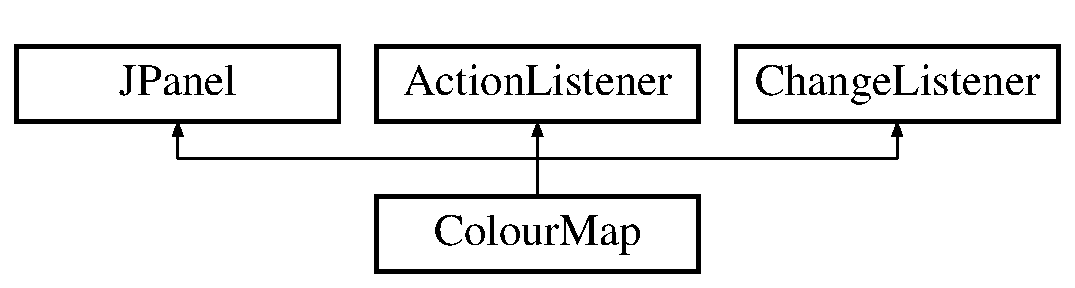
\includegraphics[height=2.000000cm]{class_colour_map}
\end{center}
\end{figure}
\subsection*{Public Member Functions}
\begin{DoxyCompactItemize}
\item 
void \hyperlink{class_colour_map_a1d41944f53775bc1a8f633063a69aca5}{action\-Performed} (Action\-Event e)
\item 
boolean \hyperlink{class_colour_map_a397ebd08df86cb0bcbc71d3e4e1ebee4}{Close\-Window} ()
\item 
\hyperlink{class_colour_map_abba281e323f79dc7dc5f31efe4b67852}{Colour\-Map} ()
\item 
boolean \hyperlink{class_colour_map_a9f696ea699b7fc471bb2dde6f1d1ce09}{Setup\-Data} (int index\-Count, Category\-Item\-Renderer renderer)
\item 
boolean \hyperlink{class_colour_map_a08978bcdc84ed70cf1139b166e37d25f}{Setup\-Data} (int index\-Count, Pie\-Plot3\-D renderer)
\item 
boolean \hyperlink{class_colour_map_a57b6f3c3f3beff5075bd82e621591138}{Setup\-Data} (int index\-Count, X\-Y\-Item\-Renderer renderer)
\item 
boolean \hyperlink{class_colour_map_a952af2354acfb507997b8fc3c38de5f7}{Setup\-Data} (int index\-Count, Default\-Polar\-Item\-Renderer renderer)
\item 
void \hyperlink{class_colour_map_a178d4ed4be0c7d2b03d2e990c9b359b0}{state\-Changed} (Change\-Event e)
\end{DoxyCompactItemize}
\subsection*{Static Public Member Functions}
\begin{DoxyCompactItemize}
\item 
static void \hyperlink{class_colour_map_a2fc22a7c0417a9538a4302be12a7004a}{main} (String\mbox{[}$\,$\mbox{]} args)
\end{DoxyCompactItemize}


\subsection{Detailed Description}
This class provides user with a choice of colours to be applied on objects from different graphs/charts/diagrams, and does all calculations needed in order to get it all working correctly. 

\begin{DoxyDate}{Date}
10 February 2013 
\end{DoxyDate}


\subsection{Constructor \& Destructor Documentation}
\hypertarget{class_colour_map_abba281e323f79dc7dc5f31efe4b67852}{\index{Colour\-Map@{Colour\-Map}!Colour\-Map@{Colour\-Map}}
\index{Colour\-Map@{Colour\-Map}!ColourMap@{Colour\-Map}}
\subsubsection[{Colour\-Map}]{\setlength{\rightskip}{0pt plus 5cm}Colour\-Map.\-Colour\-Map (
\begin{DoxyParamCaption}
{}
\end{DoxyParamCaption}
)}}\label{class_colour_map_abba281e323f79dc7dc5f31efe4b67852}
Constructor is being called to construct a new Border\-Layout and to set up the G\-U\-I. 
\begin{DoxyCode}
207                          \{
208         super( \textcolor{keyword}{new} BorderLayout(  ) );
209         setupGUI(  ); \textcolor{comment}{// Sets up the GUI}
210     \}
\end{DoxyCode}


\subsection{Member Function Documentation}
\hypertarget{class_colour_map_a1d41944f53775bc1a8f633063a69aca5}{\index{Colour\-Map@{Colour\-Map}!action\-Performed@{action\-Performed}}
\index{action\-Performed@{action\-Performed}!ColourMap@{Colour\-Map}}
\subsubsection[{action\-Performed}]{\setlength{\rightskip}{0pt plus 5cm}void Colour\-Map.\-action\-Performed (
\begin{DoxyParamCaption}
\item[{Action\-Event}]{e}
\end{DoxyParamCaption}
)}}\label{class_colour_map_a1d41944f53775bc1a8f633063a69aca5}
This method handles all the actions performed by the user. 
\begin{DoxyCode}
32                                                  \{
33         
34         \textcolor{keywordflow}{if}( e.getSource(  ) == m\_MoreColoursButton ) \{
35             \textcolor{comment}{// Show advanced colour menu}
36             
37             Color newColor = JColorChooser.showDialog( 
38                                 \hyperlink{class_colour_map}{ColourMap}.this, \textcolor{stringliteral}{"Choose Object Colour"},
39                                 m\_ObjectColour.getBackground(  ) );
40             \textcolor{keywordflow}{if}(  newColor != null ) \{
41                 m\_ObjectColour.setBackground( newColor );
42                 
43             \}
44         \}
45         
46         \textcolor{keywordflow}{else} \textcolor{keywordflow}{if}(  ( e.getSource(  ) == m\_ConfirmOK ) ||
47                   (  e.getSource(  ) == m\_ConfirmApply ) ) \{
48             \textcolor{keywordflow}{if}( m\_SchemeSelected ) \{
49                 
50             \} \textcolor{keywordflow}{else} \{
51                 \textcolor{comment}{/* This will check for the correct object, will change its colour
}
52 \textcolor{comment}{                 * and then will close the window */}
53                 \textcolor{keywordflow}{if}( getObjectType(  ).equals( m\_CategoryItemRendererName ) ) \{
54                     \textcolor{comment}{// Calls SetColour method for the CategoryItemRenderer type.}
55                     setColour( getIndexToChange(  ),getCIRToChange(  ),
56                               m\_ObjectColour.getBackground(  ) );
57                 \} \textcolor{keywordflow}{else} \textcolor{keywordflow}{if}( getObjectType(  ).equals( m\_PiePlot3DName ) ) \{
58                     \textcolor{comment}{// Calls SetColour method for the PiePlot3D type.}
59                     setColour( getIndexToChange(  ),getPP3DToChange(  ),
60                               m\_ObjectColour.getBackground(  ) );
61                 \} \textcolor{keywordflow}{else} \textcolor{keywordflow}{if}( getObjectType(  ).equals( m\_XYItemRendererName ) ) \{
62                     \textcolor{comment}{// Calls SetColour method for the XYItemRenderer type.}
63                     setColour( getIndexToChange(  ),getXYIRToChange(  ),
64                               m\_ObjectColour.getBackground(  ) );
65                 \} \textcolor{keywordflow}{else} \textcolor{keywordflow}{if}( getObjectType(  ).equals( m\_PolarItemRendererName ) ) \{
66                     \textcolor{comment}{// Calls SetColour method for the XYItemRenderer type.}
67                     setColour( getIndexToChange(  ),getPolarIRToChange(  ),
68                               m\_ObjectColour.getBackground(  ) );
69                 \} \textcolor{keywordflow}{else} \{
70                     \textcolor{comment}{/* Displays error message, if the renderer/object has not been
}
71 \textcolor{comment}{                     * recognized and/or it is missing an ActionListener condition.
}
72 \textcolor{comment}{                     */}
73                     System.out.println( m\_ObjectType );
74                     System.out.println( \textcolor{stringliteral}{"Renderer Type not recognized,"}
75                                        + \textcolor{stringliteral}{" Missing ActionListener."} );
76                 \}
77             \}
78             \textcolor{keywordflow}{if}( e.getSource(  ) == m\_ConfirmOK ) \{
79                 \textcolor{comment}{/* Closes the window if changes confirmed. */}
80                 \hyperlink{class_colour_map_a397ebd08df86cb0bcbc71d3e4e1ebee4}{CloseWindow}(  );
81             \}
82         \} \textcolor{keywordflow}{else} \textcolor{keywordflow}{if}(  e.getSource(  ) == m\_ConfirmCancel ) \{
83             \textcolor{comment}{/* Doesn't update the actual object, just closes the window. */}
84             \hyperlink{class_colour_map_a397ebd08df86cb0bcbc71d3e4e1ebee4}{CloseWindow}(  );
85         \} \textcolor{keywordflow}{else} \textcolor{keywordflow}{if}(  e.getSource(  ) == m\_IndexSelection ) \{
86             \textcolor{comment}{/* Sets the indexToChange value and updates the colour of
}
87 \textcolor{comment}{             * colour preview(  objectColour ) to match the current colour of
}
88 \textcolor{comment}{             * object on that index.
}
89 \textcolor{comment}{             */}
90              setIndexToChange( m\_IndexSelection.getSelectedIndex(  ) );
91             m\_ObjectColour.setBackground( applyPreviousColour(  ) );
92         \} \textcolor{keywordflow}{else} \textcolor{keywordflow}{if}(  e.getSource(  ) == m\_ColourSchemesBox ) \{
93             m\_SchemeSelected = \textcolor{keyword}{true};
94             m\_ColourSchemes[0][0]= Color.RED;
95             m\_ColourSchemes[0][1]= Color.GREEN;
96             m\_ColourSchemes[0][2]= Color.BLUE;
97             m\_ColourSchemes[0][3]= Color.YELLOW;
98             m\_ColourSchemes[0][4]= Color.CYAN;
99             m\_ColourSchemes[1][0]= Color.ORANGE;
100             m\_ColourSchemes[1][1]= Color.YELLOW;
101             m\_ColourSchemes[1][2]= Color.RED;
102             m\_ColourSchemes[1][3]= Color.PINK;
103             m\_ColourSchemes[1][4] = Color.MAGENTA;
104             m\_ColourSchemes[2][0] = Color.LIGHT\_GRAY;
105             m\_ColourSchemes[2][1] = Color.GRAY;
106             m\_ColourSchemes[2][2] = Color.DARK\_GRAY;
107             m\_ColourSchemes[2][3] = Color.BLACK;
108             m\_ColourSchemes[2][4] = Color.WHITE;
109             m\_ColourSchemes[3][0] = Color.CYAN;
110             m\_ColourSchemes[3][1] = Color.PINK;
111             m\_ColourSchemes[3][2]= Color.MAGENTA;
112             m\_ColourSchemes[3][3]= Color.YELLOW;
113             m\_ColourSchemes[3][4]= Color.LIGHT\_GRAY;
114             m\_ColourSchemes[4][0]= Color.CYAN;
115             m\_ColourSchemes[4][1]= Color.BLUE;
116             m\_ColourSchemes[4][2]= Color.PINK;
117             m\_ColourSchemes[4][3]= Color.MAGENTA;
118             m\_ColourSchemes[4][4]= Color.BLACK;
119             
120             \textcolor{keywordtype}{int} index = m\_ColourSchemesBox.getSelectedIndex(  );
121             
122             \textcolor{keywordflow}{if}( getObjectType(  ).equals( m\_CategoryItemRendererName ) ) \{
123                 \textcolor{comment}{// Calls SetColour method for the CategoryItemRenderer type.}
124                 \textcolor{keywordtype}{int} j=0;
125                 \textcolor{keywordflow}{for}( \textcolor{keywordtype}{int} i=0;i< getIndexCount(  ); i++ ) \{
126                     setColour( i,m\_C\_objectToChange,m\_ColourSchemes[index][j] );
127                     
128                     \textcolor{keywordflow}{if}( j<m\_ColourSchemes[index].length-1 ) \{
129                         j++;
130                     \} \textcolor{keywordflow}{else} \{
131                         j = 0;
132                     \}
133                     
134                 \}
135                 
136             \} \textcolor{keywordflow}{else} \textcolor{keywordflow}{if}( getObjectType(  ).equals( m\_PiePlot3DName ) ) \{
137                 \textcolor{comment}{// Calls SetColour method for the PiePlot3D type.}
138                 \textcolor{keywordtype}{int} j=0;
139                 \textcolor{keywordflow}{for}( \textcolor{keywordtype}{int} i=0;i< getIndexCount(  ); i++ ) \{
140                     setColour( i,m\_P\_objectToChange,m\_ColourSchemes[index][j] );
141                     
142                     \textcolor{keywordflow}{if}( j<m\_ColourSchemes[index].length-1 ) \{
143                         j++;
144                     \} \textcolor{keywordflow}{else} \{
145                         j = 0;
146                     \}
147                     
148                 \}
149             \} \textcolor{keywordflow}{else} \textcolor{keywordflow}{if}( getObjectType(  ).equals( m\_XYItemRendererName ) ) \{
150                 \textcolor{comment}{// Calls SetColour method for the XYItemRenderer type.}
151                 \textcolor{keywordtype}{int} j=0;
152                 \textcolor{keywordflow}{for}( \textcolor{keywordtype}{int} i=0;i< getIndexCount(  ); i++ ) \{
153                     setColour( i,m\_X\_objectToChange,m\_ColourSchemes[index][j] );
154                     
155                     \textcolor{keywordflow}{if}( j<m\_ColourSchemes[index].length-1 ) \{
156                         j++;
157                     \} \textcolor{keywordflow}{else} \{
158                         j = 0;
159                     \}
160                     
161                 \}
162             \} \textcolor{keywordflow}{else} \textcolor{keywordflow}{if}( getObjectType(  ).equals( m\_PolarItemRendererName ) ) \{
163                 \textcolor{comment}{// Calls SetColour method for the XYItemRenderer type.}
164                 \textcolor{keywordtype}{int} j=0;
165                 \textcolor{keywordflow}{for}( \textcolor{keywordtype}{int} i=0;i< getIndexCount(  ); i++ ) \{
166                     setColour( i,m\_PO\_objectToChange,m\_ColourSchemes[index][j] );
167                     
168                     \textcolor{keywordflow}{if}( j<m\_ColourSchemes[index].length-1 ) \{
169                         j++;
170                     \} \textcolor{keywordflow}{else} \{
171                         j = 0;
172                     \}
173                     
174                 \}
175             \} \textcolor{keywordflow}{else} \{
176                 \textcolor{comment}{/* Displays error message, if the renderer/object has not been
}
177 \textcolor{comment}{                 * recognized and/or it is missing an ActionListener condition.
}
178 \textcolor{comment}{                 */}
179                 System.out.println( m\_ObjectType );
180                 System.out.println( \textcolor{stringliteral}{"Renderer Type not recognized,"}
181                                    + \textcolor{stringliteral}{" Missing ActionListener."} );
182             \}
183         \}
184         
185         
186     \}
\end{DoxyCode}
\hypertarget{class_colour_map_a397ebd08df86cb0bcbc71d3e4e1ebee4}{\index{Colour\-Map@{Colour\-Map}!Close\-Window@{Close\-Window}}
\index{Close\-Window@{Close\-Window}!ColourMap@{Colour\-Map}}
\subsubsection[{Close\-Window}]{\setlength{\rightskip}{0pt plus 5cm}boolean Colour\-Map.\-Close\-Window (
\begin{DoxyParamCaption}
{}
\end{DoxyParamCaption}
)}}\label{class_colour_map_a397ebd08df86cb0bcbc71d3e4e1ebee4}
This method closes/hides the window without shutting down the program. It's public, just incase there is a need to close it outside this class. 
\begin{DoxyCode}
192                                    \{
193         \textcolor{keywordtype}{boolean} errorless = \textcolor{keyword}{true};
194         
195         \textcolor{keywordflow}{try} \{
196             m\_MainColourFrame.dispose(  );
197         \} \textcolor{keywordflow}{catch}(  Exception e ) \{
198             errorless = \textcolor{keyword}{false};
199         \}
200         \textcolor{keywordflow}{return} errorless;
201     \}
\end{DoxyCode}
\hypertarget{class_colour_map_a2fc22a7c0417a9538a4302be12a7004a}{\index{Colour\-Map@{Colour\-Map}!main@{main}}
\index{main@{main}!ColourMap@{Colour\-Map}}
\subsubsection[{main}]{\setlength{\rightskip}{0pt plus 5cm}static void Colour\-Map.\-main (
\begin{DoxyParamCaption}
\item[{String\mbox{[}$\,$\mbox{]}}]{args}
\end{DoxyParamCaption}
)\hspace{0.3cm}{\ttfamily [static]}}}\label{class_colour_map_a2fc22a7c0417a9538a4302be12a7004a}

\begin{DoxyCode}
1080                                              \{
1081         \textcolor{comment}{/* Unit tests */}
1082         
1083         \hyperlink{class_colour_map}{ColourMap} cM = \textcolor{keyword}{new} \hyperlink{class_colour_map_abba281e323f79dc7dc5f31efe4b67852}{ColourMap}(  );
1084         CategoryItemRenderer nullCIR = null;
1085         XYItemRenderer nullXYIR = null;
1086         PiePlot3D nullPP3D = null;
1087         
1088         
1089         System.out.println( \textcolor{stringliteral}{"SetupData CIR Test"} );
1090         System.out.println( \textcolor{stringliteral}{"Both invalid."} );
1091         cM.\hyperlink{class_colour_map_a9f696ea699b7fc471bb2dde6f1d1ce09}{SetupData}( -1, nullCIR ); \textcolor{comment}{//Both invalid inputs}
1092         System.out.println( \textcolor{stringliteral}{"Invalid Renderer."} );
1093         cM.\hyperlink{class_colour_map_a9f696ea699b7fc471bb2dde6f1d1ce09}{SetupData}( 1, nullCIR ); \textcolor{comment}{//Second input invalid}
1094         System.out.println( \textcolor{stringliteral}{"-------------------------------------------------"} );
1095         
1096         System.out.println( \textcolor{stringliteral}{"SetupData XYIR Test"} );
1097         System.out.println( \textcolor{stringliteral}{"Both invalid."} );
1098         cM.\hyperlink{class_colour_map_a9f696ea699b7fc471bb2dde6f1d1ce09}{SetupData}( -1, nullXYIR ); \textcolor{comment}{//Both invalid inputs}
1099         System.out.println( \textcolor{stringliteral}{"Invalid Renderer."} );
1100         cM.\hyperlink{class_colour_map_a9f696ea699b7fc471bb2dde6f1d1ce09}{SetupData}( 1, nullXYIR ); \textcolor{comment}{//Second input invalid}
1101         System.out.println( \textcolor{stringliteral}{"-------------------------------------------------"} );
1102         
1103         
1104         System.out.println( \textcolor{stringliteral}{"SetupData PP3D Test"} );
1105         System.out.println( \textcolor{stringliteral}{"Both invalid."} );
1106         cM.\hyperlink{class_colour_map_a9f696ea699b7fc471bb2dde6f1d1ce09}{SetupData}( -1, nullPP3D ); \textcolor{comment}{//Both invalid inputs}
1107         System.out.println( \textcolor{stringliteral}{"Invalid Renderer."} );
1108         cM.\hyperlink{class_colour_map_a9f696ea699b7fc471bb2dde6f1d1ce09}{SetupData}( 1, nullPP3D ); \textcolor{comment}{//Second input invalid}
1109         System.out.println( \textcolor{stringliteral}{"-------------------------------------------------"} );
1110         
1111         System.out.println( \textcolor{stringliteral}{"setColour PP3D Test"} );
1112         System.out.println( \textcolor{stringliteral}{"All invalid."} );
1113         cM.setColour( -1, nullPP3D, null );
1114         System.out.println( \textcolor{stringliteral}{"Invalid Renderer."} );
1115         cM.setColour( 1, nullPP3D, Color.YELLOW );
1116         System.out.println( \textcolor{stringliteral}{"-------------------------------------------------"} );
1117         
1118         System.out.println( \textcolor{stringliteral}{"setColour CIR Test"} );
1119         System.out.println( \textcolor{stringliteral}{"All invalid."} );
1120         cM.setColour( -1, nullCIR, null );
1121         System.out.println( \textcolor{stringliteral}{"Invalid Renderer."} );
1122         cM.setColour( 1, nullCIR, Color.YELLOW );
1123         System.out.println( \textcolor{stringliteral}{"-------------------------------------------------"} );
1124         
1125         System.out.println( \textcolor{stringliteral}{"setColour XYIR Test"} );
1126         System.out.println( \textcolor{stringliteral}{"All invalid."} );
1127         cM.setColour( -1, nullXYIR, null );
1128         System.out.println( \textcolor{stringliteral}{"Invalid Renderer."} );
1129         cM.setColour( 1, nullXYIR, Color.YELLOW );
1130         System.out.println( \textcolor{stringliteral}{"-------------------------------------------------"} );
1131         
1132         System.out.println( \textcolor{stringliteral}{"setIndexCount Test"} );
1133         System.out.println( \textcolor{stringliteral}{"Invalid input."} );
1134         cM.setIndexCount( -1 );
1135         System.out.println( \textcolor{stringliteral}{"Valid"} );
1136         cM.setIndexCount( 3 );
1137         System.out.println( \textcolor{stringliteral}{"-------------------------------------------------"} );
1138         
1139         System.out.println( \textcolor{stringliteral}{"setIndexToChange Test"} );
1140         System.out.println( \textcolor{stringliteral}{"Invalid input."} );
1141         cM.setIndexToChange( -1 );
1142         System.out.println( \textcolor{stringliteral}{"Valid"} );
1143         cM.setIndexToChange( 3 );
1144         System.out.println( \textcolor{stringliteral}{"-------------------------------------------------"} );
1145         
1146         System.out.println( \textcolor{stringliteral}{"setObjectToChange CIR Test"} );
1147         System.out.println( \textcolor{stringliteral}{"Invalid input."} );
1148         cM.setObjectToChange( nullCIR );
1149         System.out.println( \textcolor{stringliteral}{"-------------------------------------------------"} );
1150         
1151         System.out.println( \textcolor{stringliteral}{"setObjectToChange XYIR Test"} );
1152         System.out.println( \textcolor{stringliteral}{"Invalid input."} );
1153         cM.setObjectToChange( nullXYIR );
1154         System.out.println( \textcolor{stringliteral}{"-------------------------------------------------"} );
1155         
1156         System.out.println( \textcolor{stringliteral}{"setObjectToChange PP3D Test"} );
1157         System.out.println( \textcolor{stringliteral}{"Invalid input."} );
1158         cM.setObjectToChange( nullPP3D );
1159         System.out.println( \textcolor{stringliteral}{"-------------------------------------------------"} );
1160         
1161         System.out.println( \textcolor{stringliteral}{"setObjectType Test"} );
1162         System.out.println( \textcolor{stringliteral}{"Invalid input."} );
1163         cM.setObjectType( \textcolor{stringliteral}{""} );
1164         cM.setObjectType( null );
1165         System.out.println( \textcolor{stringliteral}{"Valid"} );
1166         cM.setObjectType( \textcolor{stringliteral}{"Tram!"} );
1167         System.out.println( \textcolor{stringliteral}{"-------------------------------------------------"} );
1168     \}
\end{DoxyCode}
\hypertarget{class_colour_map_a9f696ea699b7fc471bb2dde6f1d1ce09}{\index{Colour\-Map@{Colour\-Map}!Setup\-Data@{Setup\-Data}}
\index{Setup\-Data@{Setup\-Data}!ColourMap@{Colour\-Map}}
\subsubsection[{Setup\-Data}]{\setlength{\rightskip}{0pt plus 5cm}boolean Colour\-Map.\-Setup\-Data (
\begin{DoxyParamCaption}
\item[{int}]{index\-Count, }
\item[{Category\-Item\-Renderer}]{renderer}
\end{DoxyParamCaption}
)}}\label{class_colour_map_a9f696ea699b7fc471bb2dde6f1d1ce09}
This method sets up all the needed data to perform colour changes with the Category\-Item\-Renderer type object. 
\begin{DoxyParams}{Parameters}
{\em index\-Count} & contains number of indexes the object has. \\
\hline
{\em renderer} & contains the object which needs colour adjustments. \\
\hline
\end{DoxyParams}
\begin{DoxyReturn}{Returns}
Returns true if it executed without errors, false otherwise. 
\end{DoxyReturn}

\begin{DoxyCode}
219                                                                               \{
220         \textcolor{keywordtype}{boolean} errorless = \textcolor{keyword}{true};
221         
222         \textcolor{keywordflow}{if}( indexCount < 0 ) \{
223             \textcolor{comment}{/* Checks if the index count is a negative number.
}
224 \textcolor{comment}{             * If true, returns an error message. */}
225             System.out.println( \textcolor{stringliteral}{"SetupData ERROR:"} );
226             System.out.println( \textcolor{stringliteral}{"Trying to set indexCount to a negative number. "}
227                                + \textcolor{stringliteral}{"Index count can't be negative."} );
228             errorless = \textcolor{keyword}{false};
229         \}
230         
231         \textcolor{keywordflow}{if}(  renderer == null ) \{
232             \textcolor{comment}{/* Checks if the renderer is null.
}
233 \textcolor{comment}{             * If true, returns an error message. */}
234             System.out.println( \textcolor{stringliteral}{"SetupData ERROR:"} );
235             System.out.println( \textcolor{stringliteral}{"Renderer passed in is of a null value. "}
236                                + \textcolor{stringliteral}{"Renderer can't be null."} );
237             errorless = \textcolor{keyword}{false};
238         \}
239         
240         \textcolor{keywordflow}{if}( errorless ) \{
241             \textcolor{comment}{/* If there are no errors detected in the passed in data,
}
242 \textcolor{comment}{             * Initialize all of it and create the GUI. */}
243             setObjectToChange( renderer );
244             setIndexCount( indexCount );
245             setObjectType( m\_CategoryItemRendererName );
246             
247             createAndShowGUI(  );
248         \}
249         
250         \textcolor{keywordflow}{return} errorless;
251     \}
\end{DoxyCode}
\hypertarget{class_colour_map_a08978bcdc84ed70cf1139b166e37d25f}{\index{Colour\-Map@{Colour\-Map}!Setup\-Data@{Setup\-Data}}
\index{Setup\-Data@{Setup\-Data}!ColourMap@{Colour\-Map}}
\subsubsection[{Setup\-Data}]{\setlength{\rightskip}{0pt plus 5cm}boolean Colour\-Map.\-Setup\-Data (
\begin{DoxyParamCaption}
\item[{int}]{index\-Count, }
\item[{Pie\-Plot3\-D}]{renderer}
\end{DoxyParamCaption}
)}}\label{class_colour_map_a08978bcdc84ed70cf1139b166e37d25f}
This method sets up all the needed data to perform colour changes with the Pie\-Plot3\-D type object. 
\begin{DoxyParams}{Parameters}
{\em index\-Count} & contains number of indexes the object has. \\
\hline
{\em renderer} & contains the object which needs colour adjustments. \\
\hline
\end{DoxyParams}
\begin{DoxyReturn}{Returns}
Returns true if it executed without errors, false otherwise. 
\end{DoxyReturn}

\begin{DoxyCode}
260                                                                    \{
261         \textcolor{keywordtype}{boolean} errorless = \textcolor{keyword}{true};
262         
263         \textcolor{keywordflow}{if}( indexCount < 0 ) \{
264             \textcolor{comment}{/* Checks if the index count is a negative number.
}
265 \textcolor{comment}{             * If true, returns an error message. */}
266             System.out.println( \textcolor{stringliteral}{"SetupData ERROR:"} );
267             System.out.println( \textcolor{stringliteral}{"Trying to set indexCount to a negative number. "}
268                                + \textcolor{stringliteral}{"Index count can't be negative."} );
269             errorless = \textcolor{keyword}{false};
270         \}
271         
272         \textcolor{keywordflow}{if}( renderer == null ) \{
273             \textcolor{comment}{/* Checks if the renderer is null.
}
274 \textcolor{comment}{             * If true, returns an error message. */}
275             System.out.println( \textcolor{stringliteral}{"SetupData ERROR:"} );
276             System.out.println( \textcolor{stringliteral}{"Renderer passed in is of a null value. "}
277                                + \textcolor{stringliteral}{"Renderer can't be null."} );
278             errorless = \textcolor{keyword}{false};
279         \}
280         
281         \textcolor{keywordflow}{if}( errorless )\{
282             \textcolor{comment}{/* If there are no errors detected in the passed in data,
}
283 \textcolor{comment}{             * Initialize all of it and create the GUI. */}
284             setObjectToChange( renderer );
285             setIndexCount( indexCount );
286             setObjectType( m\_PiePlot3DName );
287             
288             createAndShowGUI(  );
289         \}
290         
291         \textcolor{keywordflow}{return} errorless;
292     \}
\end{DoxyCode}
\hypertarget{class_colour_map_a57b6f3c3f3beff5075bd82e621591138}{\index{Colour\-Map@{Colour\-Map}!Setup\-Data@{Setup\-Data}}
\index{Setup\-Data@{Setup\-Data}!ColourMap@{Colour\-Map}}
\subsubsection[{Setup\-Data}]{\setlength{\rightskip}{0pt plus 5cm}boolean Colour\-Map.\-Setup\-Data (
\begin{DoxyParamCaption}
\item[{int}]{index\-Count, }
\item[{X\-Y\-Item\-Renderer}]{renderer}
\end{DoxyParamCaption}
)}}\label{class_colour_map_a57b6f3c3f3beff5075bd82e621591138}
This method sets up all the needed data to perform colour changes with the X\-Y\-Item\-Renderer type object. 
\begin{DoxyParams}{Parameters}
{\em index\-Count} & contains number of indexes the object has. \\
\hline
{\em renderer} & contains the object which needs colour adjustments. \\
\hline
\end{DoxyParams}
\begin{DoxyReturn}{Returns}
Returns true if it executed without errors, false otherwise. 
\end{DoxyReturn}

\begin{DoxyCode}
302                                                        \{
303         Boolean errorless = \textcolor{keyword}{true};
304         \textcolor{keywordflow}{if}( indexCount < 0 ) \{
305             \textcolor{comment}{/* Checks if the index count is a negative number.
}
306 \textcolor{comment}{             * If true, returns an error message. */}
307             System.out.println( \textcolor{stringliteral}{"SetupData ERROR:"} );
308             System.out.println( \textcolor{stringliteral}{"Trying to set indexCount to a negative number. "}
309                     + \textcolor{stringliteral}{"Index count can't be negative."} );
310             errorless = \textcolor{keyword}{false};
311         \}
312         
313         \textcolor{keywordflow}{if}(  renderer == null ) \{
314             \textcolor{comment}{/* Checks if the renderer is null.
}
315 \textcolor{comment}{             * If true, returns an error message. */}
316             System.out.println( \textcolor{stringliteral}{"SetupData ERROR:"} );
317             System.out.println( \textcolor{stringliteral}{"Renderer passed in is of a null value. "}
318                                + \textcolor{stringliteral}{"Renderer can't be null."} );
319             errorless = \textcolor{keyword}{false};
320         \}
321         
322         \textcolor{keywordflow}{if}( errorless ) \{
323             \textcolor{comment}{/* If there are no errors detected in the passed in data,
}
324 \textcolor{comment}{             * Initialize all of it and create the GUI. */}
325             setObjectToChange( renderer );
326             setIndexCount( indexCount );
327             setObjectType( m\_XYItemRendererName );
328             
329             createAndShowGUI(  );
330         \}
331         
332         \textcolor{keywordflow}{return} errorless;
333     \}
\end{DoxyCode}
\hypertarget{class_colour_map_a952af2354acfb507997b8fc3c38de5f7}{\index{Colour\-Map@{Colour\-Map}!Setup\-Data@{Setup\-Data}}
\index{Setup\-Data@{Setup\-Data}!ColourMap@{Colour\-Map}}
\subsubsection[{Setup\-Data}]{\setlength{\rightskip}{0pt plus 5cm}boolean Colour\-Map.\-Setup\-Data (
\begin{DoxyParamCaption}
\item[{int}]{index\-Count, }
\item[{Default\-Polar\-Item\-Renderer}]{renderer}
\end{DoxyParamCaption}
)}}\label{class_colour_map_a952af2354acfb507997b8fc3c38de5f7}
This method sets up all the needed data to perform colour changes with the X\-Y\-Item\-Renderer type object. 
\begin{DoxyParams}{Parameters}
{\em index\-Count} & contains number of indexes the object has. \\
\hline
{\em renderer} & contains the object which needs colour adjustments. \\
\hline
\end{DoxyParams}
\begin{DoxyReturn}{Returns}
Returns true if it executed without errors, false otherwise. 
\end{DoxyReturn}

\begin{DoxyCode}
343                                                 \{
344         Boolean errorless = \textcolor{keyword}{true};
345         \textcolor{keywordflow}{if}( indexCount < 0 ) \{
346             \textcolor{comment}{/* Checks if the index count is a negative number.
}
347 \textcolor{comment}{             * If true, returns an error message. */}
348             System.out.println( \textcolor{stringliteral}{"SetupData ERROR:"} );
349             System.out.println( \textcolor{stringliteral}{"Trying to set indexCount to a negative number. "}
350                     + \textcolor{stringliteral}{"Index count can't be negative."} );
351             errorless = \textcolor{keyword}{false};
352         \}
353         
354         \textcolor{keywordflow}{if}(  renderer == null ) \{
355             \textcolor{comment}{/* Checks if the renderer is null.
}
356 \textcolor{comment}{             * If true, returns an error message. */}
357             System.out.println( \textcolor{stringliteral}{"SetupData ERROR:"} );
358             System.out.println( \textcolor{stringliteral}{"Renderer passed in is of a null value. "}
359                                + \textcolor{stringliteral}{"Renderer can't be null."} );
360             errorless = \textcolor{keyword}{false};
361         \}
362         
363         \textcolor{keywordflow}{if}( errorless ) \{
364             \textcolor{comment}{/* If there are no errors detected in the passed in data,
}
365 \textcolor{comment}{             * Initialize all of it and create the GUI. */}
366             setObjectToChange( renderer );
367             setIndexCount( indexCount );
368             setObjectType( m\_PolarItemRendererName );
369             
370             createAndShowGUI(  );
371         \}
372         
373         \textcolor{keywordflow}{return} errorless;
374     \}
\end{DoxyCode}
\hypertarget{class_colour_map_a178d4ed4be0c7d2b03d2e990c9b359b0}{\index{Colour\-Map@{Colour\-Map}!state\-Changed@{state\-Changed}}
\index{state\-Changed@{state\-Changed}!ColourMap@{Colour\-Map}}
\subsubsection[{state\-Changed}]{\setlength{\rightskip}{0pt plus 5cm}void Colour\-Map.\-state\-Changed (
\begin{DoxyParamCaption}
\item[{Change\-Event}]{e}
\end{DoxyParamCaption}
)}}\label{class_colour_map_a178d4ed4be0c7d2b03d2e990c9b359b0}
This method is responsible for detecting when the state of the button has changed, thus responding to it with an action. 
\begin{DoxyParams}{Parameters}
{\em e} & is a Change\-Event type of event. \\
\hline
\end{DoxyParams}

\begin{DoxyCode}
382                                               \{
383         \textcolor{comment}{//Changes colour depending on what user has clicked}
384         Color newColor = m\_MoreColours.getColor(  );
385         m\_ObjectColour.setBackground( newColor );
386     \}
\end{DoxyCode}


The documentation for this class was generated from the following file\-:\begin{DoxyCompactItemize}
\item 
\hyperlink{_colour_map_8java}{Colour\-Map.\-java}\end{DoxyCompactItemize}

\hypertarget{class_column_chart}{\section{Column\-Chart Class Reference}
\label{class_column_chart}\index{Column\-Chart@{Column\-Chart}}
}


A class that displays specific data in a Column \hyperlink{interface_chart}{Chart} visualiser.  


Inheritance diagram for Column\-Chart\-:\begin{figure}[H]
\begin{center}
\leavevmode
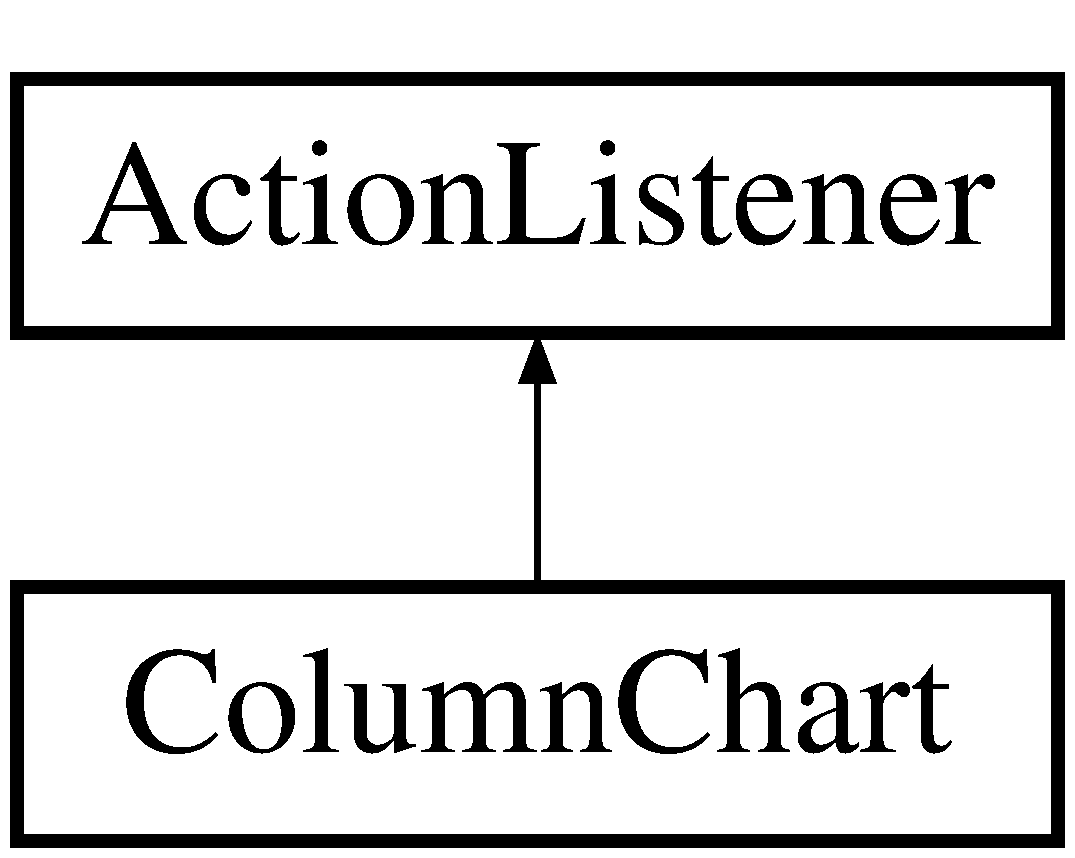
\includegraphics[height=2.000000cm]{class_column_chart}
\end{center}
\end{figure}
\subsection*{Public Member Functions}
\begin{DoxyCompactItemize}
\item 
\hyperlink{class_column_chart_a4c421ca57f3eb716949c9e5b06507c3c}{Column\-Chart} (String\mbox{[}$\,$\mbox{]}\mbox{[}$\,$\mbox{]} data, \hyperlink{class_dataset}{Dataset} dataset, \hyperlink{class_data_attribute}{Data\-Attribute} setting)
\item 
\hyperlink{class_column_chart_a40f6cc800cef38dde9befc3e24686cc2}{Column\-Chart} (String\mbox{[}$\,$\mbox{]}\mbox{[}$\,$\mbox{]} data, \hyperlink{class_dataset}{Dataset} dataset, \hyperlink{class_data_attribute}{Data\-Attribute} setting, String\mbox{[}$\,$\mbox{]}\mbox{[}$\,$\mbox{]} second\-Data, \hyperlink{class_dataset}{Dataset} second\-Dataset, \hyperlink{class_data_attribute}{Data\-Attribute} second\-Setting)
\item 
\hyperlink{class_column_chart_a8e580c4c64b84f623403bd113d8af320}{Column\-Chart} (\hyperlink{class_data_attribute}{Data\-Attribute} setting)
\item 
\hyperlink{class_column_chart_a6beb1983d5766b94f56c8f91f2a93ef4}{Column\-Chart} (\hyperlink{class_data_attribute}{Data\-Attribute} setting, \hyperlink{class_data_attribute}{Data\-Attribute} secondsetting)
\item 
boolean \hyperlink{class_column_chart_add2a600244d03013679b95eb8f29f09d}{Set\-Chart\-Title} (String Chart\-Title)
\item 
boolean \hyperlink{class_column_chart_a35cb0aa2a3888f2f02fe4994842a5741}{Set\-Second\-Chart\-Title} (String Chart\-Title)
\item 
void \hyperlink{class_column_chart_aae904321080912d1df80692320b583b5}{action\-Performed} (Action\-Event e)
\end{DoxyCompactItemize}
\subsection*{Static Public Member Functions}
\begin{DoxyCompactItemize}
\item 
static void \hyperlink{class_column_chart_a078fed3c67b6b8b05cc8fe75c6bcb4eb}{main} (String\mbox{[}$\,$\mbox{]} args)
\end{DoxyCompactItemize}


\subsection{Detailed Description}
A class that displays specific data in a Column \hyperlink{interface_chart}{Chart} visualiser. 

\begin{DoxyDate}{Date}
30/04/2013 
\end{DoxyDate}
\begin{DoxySeeAlso}{See Also}
\hyperlink{_dataset_8java}{Dataset.\-java}, \hyperlink{_bob_viz_8java}{Bob\-Viz.\-java} 
\end{DoxySeeAlso}


\subsection{Constructor \& Destructor Documentation}
\hypertarget{class_column_chart_a4c421ca57f3eb716949c9e5b06507c3c}{\index{Column\-Chart@{Column\-Chart}!Column\-Chart@{Column\-Chart}}
\index{Column\-Chart@{Column\-Chart}!ColumnChart@{Column\-Chart}}
\subsubsection[{Column\-Chart}]{\setlength{\rightskip}{0pt plus 5cm}Column\-Chart.\-Column\-Chart (
\begin{DoxyParamCaption}
\item[{String}]{data\mbox{[}$\,$\mbox{]}\mbox{[}$\,$\mbox{]}, }
\item[{{\bf Dataset}}]{dataset, }
\item[{{\bf Data\-Attribute}}]{setting}
\end{DoxyParamCaption}
)}}\label{class_column_chart_a4c421ca57f3eb716949c9e5b06507c3c}
Create a constructor taking in the following parameters\-: 
\begin{DoxyParams}{Parameters}
{\em String\mbox{[}$\,$\mbox{]}\mbox{[}$\,$\mbox{]}} & data -\/ data used to create the visualisation. \\
\hline
{\em \hyperlink{class_dataset}{Dataset}} & dataset -\/ the dataset used (rows and columns) \\
\hline
{\em \hyperlink{class_data_attribute}{Data\-Attribute}} & setting -\/ Data attributes Create the column chart dataset and instantiate it. J\-Free\-Chart. \\
\hline
\end{DoxyParams}

\begin{DoxyCode}
44                                                 \{
45         
46         m\_Data = data;
47         m\_Setting = setting;
48         m\_ChartTitle = setting.\hyperlink{class_data_attribute_ade9747a192ba22fe1020e874bff6a48c}{GetTitle}();
49         m\_XLabel = setting.\hyperlink{class_data_attribute_aecb451704a87d77dd80dbad8a19099d1}{GetAxisLabelX}();
50         m\_YLabel = setting.\hyperlink{class_data_attribute_af5f68794cd0195d42135d5e48120ccc0}{GetAxisLabelY}();
51         m\_Row = dataset.\hyperlink{class_dataset_a91257a605317576e87e1c32e54739e51}{GetNoOfRows}();
52         m\_C1 = setting.\hyperlink{class_data_attribute_a0f4a54973bc44b0526f78bda945dc81b}{GetSelectedXIndex}();
53         m\_C2 = setting.\hyperlink{class_data_attribute_a82e7519853d9f470ea183dd0c39a03d6}{GetSelectedYIndex}();
54         
55         m\_XMin = setting.\hyperlink{class_data_attribute_afa9da883abc4abad5f64c045de114c50}{GetXAxisMin}();
56         m\_XMax = setting.\hyperlink{class_data_attribute_a81243eb8f7008e05e74b0f3571d2f08d}{GetYAxisMax}();
57         m\_XScale = setting.\hyperlink{class_data_attribute_a5a1de25600487aa958a19ce01151fea4}{GetXAxisScale}();
58         m\_YScale = setting.\hyperlink{class_data_attribute_a95259727ce91efc0e0eaa28487d944c5}{GetYAxisScale}();
59 
60         CreateDataset( m\_Data );
61         ShowGraph( m\_Dataset );
62         
63     \}   
\end{DoxyCode}
\hypertarget{class_column_chart_a40f6cc800cef38dde9befc3e24686cc2}{\index{Column\-Chart@{Column\-Chart}!Column\-Chart@{Column\-Chart}}
\index{Column\-Chart@{Column\-Chart}!ColumnChart@{Column\-Chart}}
\subsubsection[{Column\-Chart}]{\setlength{\rightskip}{0pt plus 5cm}Column\-Chart.\-Column\-Chart (
\begin{DoxyParamCaption}
\item[{String}]{data\mbox{[}$\,$\mbox{]}\mbox{[}$\,$\mbox{]}, }
\item[{{\bf Dataset}}]{dataset, }
\item[{{\bf Data\-Attribute}}]{setting, }
\item[{String}]{second\-Data\mbox{[}$\,$\mbox{]}\mbox{[}$\,$\mbox{]}, }
\item[{{\bf Dataset}}]{second\-Dataset, }
\item[{{\bf Data\-Attribute}}]{second\-Setting}
\end{DoxyParamCaption}
)}}\label{class_column_chart_a40f6cc800cef38dde9befc3e24686cc2}
Create a constructor taking in the following parameters\-: 
\begin{DoxyParams}{Parameters}
{\em String\mbox{[}$\,$\mbox{]}\mbox{[}$\,$\mbox{]}} & data -\/ data used to create the visualisation. \\
\hline
{\em \hyperlink{class_dataset}{Dataset}} & dataset -\/ the dataset used (rows and columns) \\
\hline
{\em \hyperlink{class_data_attribute}{Data\-Attribute}} & setting -\/ Data attributes \\
\hline
{\em String\mbox{[}$\,$\mbox{]}\mbox{[}$\,$\mbox{]}} & second\-Data -\/ second data used to create the visualisation. \\
\hline
{\em \hyperlink{class_dataset}{Dataset}} & second\-Dataset -\/ the second dataset used (rows and columns) \\
\hline
{\em \hyperlink{class_data_attribute}{Data\-Attribute}} & second\-Setting -\/ Second Data attributes\\
\hline
\end{DoxyParams}
Create both column chart datasets and instantiate it. J\-Free\-Chart. 
\begin{DoxyCode}
80                                          \{
81 
82         m\_Data = data;
83         m\_SecondData = secondData;
84         
85         m\_Setting = setting;
86         m\_SecondSetting = secondSetting;
87         
88         m\_ChartTitle = setting.\hyperlink{class_data_attribute_ade9747a192ba22fe1020e874bff6a48c}{GetTitle}();
89         m\_SecondChartTitle = secondSetting.\hyperlink{class_data_attribute_a4079522c93025fce7569eaed585f4aeb}{GetSecondTitle}();
90         
91         m\_XLabel = setting.\hyperlink{class_data_attribute_aecb451704a87d77dd80dbad8a19099d1}{GetAxisLabelX}();
92         m\_YLabel = setting.\hyperlink{class_data_attribute_af5f68794cd0195d42135d5e48120ccc0}{GetAxisLabelY}();
93         m\_Row = dataset.\hyperlink{class_dataset_a91257a605317576e87e1c32e54739e51}{GetNoOfRows}();
94         m\_C1 = setting.\hyperlink{class_data_attribute_a0f4a54973bc44b0526f78bda945dc81b}{GetSelectedXIndex}();
95         m\_C2 = setting.\hyperlink{class_data_attribute_a82e7519853d9f470ea183dd0c39a03d6}{GetSelectedYIndex}();
96         
97         m\_SecondXLabel = secondSetting.\hyperlink{class_data_attribute_a8ace4cb1fee9e2abeabe3efc9a190c8f}{GetSecondAxisLabelX}();
98         m\_SecondYLabel = secondSetting.\hyperlink{class_data_attribute_a6efb7e067317898feefbbf6bd472b998}{GetSecondAxisLabelY}();
99         m\_SecondRow = secondDataset.\hyperlink{class_dataset_a91257a605317576e87e1c32e54739e51}{GetNoOfRows}();    
100         m\_SecondC1 = secondSetting.\hyperlink{class_data_attribute_a7f501790eee650ddf9ac17c4f63a3995}{GetSecondSelectedXIndex}();
101         m\_SecondC2 = secondSetting.\hyperlink{class_data_attribute_a6f61ad05915f4aa31ad3dba00596da64}{GetSecondSelectedYIndex}();
102 
103         m\_XMin = setting.\hyperlink{class_data_attribute_afa9da883abc4abad5f64c045de114c50}{GetXAxisMin}();
104         m\_XMax = setting.\hyperlink{class_data_attribute_a81243eb8f7008e05e74b0f3571d2f08d}{GetYAxisMax}();
105         m\_XScale = setting.\hyperlink{class_data_attribute_a5a1de25600487aa958a19ce01151fea4}{GetXAxisScale}();
106         m\_YScale = setting.\hyperlink{class_data_attribute_a95259727ce91efc0e0eaa28487d944c5}{GetYAxisScale}();
107 
108         CreateDataset( m\_Data );
109         CreateSecondDataset( m\_SecondData );
110         ShowGraph( m\_Dataset, m\_SecondDataset);
111     \}   
\end{DoxyCode}
\hypertarget{class_column_chart_a8e580c4c64b84f623403bd113d8af320}{\index{Column\-Chart@{Column\-Chart}!Column\-Chart@{Column\-Chart}}
\index{Column\-Chart@{Column\-Chart}!ColumnChart@{Column\-Chart}}
\subsubsection[{Column\-Chart}]{\setlength{\rightskip}{0pt plus 5cm}Column\-Chart.\-Column\-Chart (
\begin{DoxyParamCaption}
\item[{{\bf Data\-Attribute}}]{setting}
\end{DoxyParamCaption}
)}}\label{class_column_chart_a8e580c4c64b84f623403bd113d8af320}
constructor for J\-Unit Tests 
\begin{DoxyParams}{Parameters}
{\em setting} & \\
\hline
\end{DoxyParams}

\begin{DoxyCode}
116                                               \{
117         m\_ChartTitle = setting.\hyperlink{class_data_attribute_ade9747a192ba22fe1020e874bff6a48c}{GetTitle}();
118         m\_Setting = setting;
119         m\_XLabel = setting.\hyperlink{class_data_attribute_aecb451704a87d77dd80dbad8a19099d1}{GetAxisLabelX}();
120         m\_YLabel = setting.\hyperlink{class_data_attribute_af5f68794cd0195d42135d5e48120ccc0}{GetAxisLabelY}();
121         m\_C1 = setting.\hyperlink{class_data_attribute_a0f4a54973bc44b0526f78bda945dc81b}{GetSelectedXIndex}();
122         m\_C2 = setting.\hyperlink{class_data_attribute_a82e7519853d9f470ea183dd0c39a03d6}{GetSelectedYIndex}();
123         m\_XMin = setting.\hyperlink{class_data_attribute_afa9da883abc4abad5f64c045de114c50}{GetXAxisMin}();
124         m\_XMax = setting.\hyperlink{class_data_attribute_ada370712422c7cbd21b7be4a0d88caf7}{GetXAxisMax}();
125         m\_YMin = setting.\hyperlink{class_data_attribute_af0786b4de674874c0bb8ca9dbe1519c6}{GetYAxisMin}();
126         m\_YMax = setting.\hyperlink{class_data_attribute_a81243eb8f7008e05e74b0f3571d2f08d}{GetYAxisMax}();
127         m\_XScale = setting.\hyperlink{class_data_attribute_a5a1de25600487aa958a19ce01151fea4}{GetXAxisScale}();
128         m\_YScale = setting.\hyperlink{class_data_attribute_a95259727ce91efc0e0eaa28487d944c5}{GetYAxisScale}();
129     \}
\end{DoxyCode}
\hypertarget{class_column_chart_a6beb1983d5766b94f56c8f91f2a93ef4}{\index{Column\-Chart@{Column\-Chart}!Column\-Chart@{Column\-Chart}}
\index{Column\-Chart@{Column\-Chart}!ColumnChart@{Column\-Chart}}
\subsubsection[{Column\-Chart}]{\setlength{\rightskip}{0pt plus 5cm}Column\-Chart.\-Column\-Chart (
\begin{DoxyParamCaption}
\item[{{\bf Data\-Attribute}}]{setting, }
\item[{{\bf Data\-Attribute}}]{secondsetting}
\end{DoxyParamCaption}
)}}\label{class_column_chart_a6beb1983d5766b94f56c8f91f2a93ef4}
second constructor for J\-Unit Tests 
\begin{DoxyParams}{Parameters}
{\em setting} & \\
\hline
{\em second\-Setting} & \\
\hline
\end{DoxyParams}

\begin{DoxyCode}
135                                                                            \{
136         m\_ChartTitle = setting.\hyperlink{class_data_attribute_ade9747a192ba22fe1020e874bff6a48c}{GetTitle}();
137         m\_Setting = setting;
138         m\_XLabel = setting.\hyperlink{class_data_attribute_aecb451704a87d77dd80dbad8a19099d1}{GetAxisLabelX}();
139         m\_YLabel = setting.\hyperlink{class_data_attribute_af5f68794cd0195d42135d5e48120ccc0}{GetAxisLabelY}();
140         m\_C1 = setting.\hyperlink{class_data_attribute_a0f4a54973bc44b0526f78bda945dc81b}{GetSelectedXIndex}();
141         m\_C2 = setting.\hyperlink{class_data_attribute_a82e7519853d9f470ea183dd0c39a03d6}{GetSelectedYIndex}();
142         m\_XMin = setting.\hyperlink{class_data_attribute_afa9da883abc4abad5f64c045de114c50}{GetXAxisMin}();
143         m\_XMax = setting.\hyperlink{class_data_attribute_ada370712422c7cbd21b7be4a0d88caf7}{GetXAxisMax}();
144         m\_YMin = setting.\hyperlink{class_data_attribute_af0786b4de674874c0bb8ca9dbe1519c6}{GetYAxisMin}();
145         m\_YMax = setting.\hyperlink{class_data_attribute_a81243eb8f7008e05e74b0f3571d2f08d}{GetYAxisMax}();
146         m\_XScale = setting.\hyperlink{class_data_attribute_a5a1de25600487aa958a19ce01151fea4}{GetXAxisScale}();
147         m\_YScale = setting.\hyperlink{class_data_attribute_a95259727ce91efc0e0eaa28487d944c5}{GetYAxisScale}();
148         
149         m\_SecondChartTitle = secondsetting.\hyperlink{class_data_attribute_a4079522c93025fce7569eaed585f4aeb}{GetSecondTitle}();
150         m\_SecondSetting = secondsetting;
151         m\_SecondXLabel = secondsetting.\hyperlink{class_data_attribute_a8ace4cb1fee9e2abeabe3efc9a190c8f}{GetSecondAxisLabelX}();
152         m\_SecondYLabel = secondsetting.\hyperlink{class_data_attribute_a6efb7e067317898feefbbf6bd472b998}{GetSecondAxisLabelY}();
153         m\_SecondC1 = secondsetting.\hyperlink{class_data_attribute_a7f501790eee650ddf9ac17c4f63a3995}{GetSecondSelectedXIndex}();
154         m\_SecondC2 = secondsetting.\hyperlink{class_data_attribute_a6f61ad05915f4aa31ad3dba00596da64}{GetSecondSelectedYIndex}();;
155     \}
\end{DoxyCode}


\subsection{Member Function Documentation}
\hypertarget{class_column_chart_aae904321080912d1df80692320b583b5}{\index{Column\-Chart@{Column\-Chart}!action\-Performed@{action\-Performed}}
\index{action\-Performed@{action\-Performed}!ColumnChart@{Column\-Chart}}
\subsubsection[{action\-Performed}]{\setlength{\rightskip}{0pt plus 5cm}void Column\-Chart.\-action\-Performed (
\begin{DoxyParamCaption}
\item[{Action\-Event}]{e}
\end{DoxyParamCaption}
)}}\label{class_column_chart_aae904321080912d1df80692320b583b5}

\begin{DoxyCode}
303                                                  \{
304         \textcolor{keywordflow}{if}( e.getSource() == m\_ColChangeButton ) \{
305             \hyperlink{class_colour_map}{ColourMap} cM = \textcolor{keyword}{new} \hyperlink{class_colour_map}{ColourMap}();
306             cM.\hyperlink{class_colour_map_a9f696ea699b7fc471bb2dde6f1d1ce09}{SetupData}( m\_IndexCount, m\_Renderer );
307             cM.setVisible( \textcolor{keyword}{false} );
308         \}
309     \}
\end{DoxyCode}
\hypertarget{class_column_chart_a078fed3c67b6b8b05cc8fe75c6bcb4eb}{\index{Column\-Chart@{Column\-Chart}!main@{main}}
\index{main@{main}!ColumnChart@{Column\-Chart}}
\subsubsection[{main}]{\setlength{\rightskip}{0pt plus 5cm}static void Column\-Chart.\-main (
\begin{DoxyParamCaption}
\item[{String\mbox{[}$\,$\mbox{]}}]{args}
\end{DoxyParamCaption}
)\hspace{0.3cm}{\ttfamily [static]}}}\label{class_column_chart_a078fed3c67b6b8b05cc8fe75c6bcb4eb}
main method to carry out J\-Unit Tests 
\begin{DoxyCode}
388                                               \{
389         \textcolor{comment}{// Test to display a single chart}
390         \hyperlink{class_data_attribute}{DataAttribute} test = \hyperlink{class_data_attribute}{DataAttribute}.
      \hyperlink{class_data_attribute_a9c7a1923698c1530fa38c959596199bc}{GetTestDataAttribute}();
391         \hyperlink{class_column_chart}{ColumnChart} columnTest = \textcolor{keyword}{new} \hyperlink{class_column_chart_a4c421ca57f3eb716949c9e5b06507c3c}{ColumnChart}(test);
392         
393         Random generator = \textcolor{keyword}{new} Random();
394         
395         XYSeriesCollection dataSeries = \textcolor{keyword}{new} XYSeriesCollection();
396         XYSeries dataset = \textcolor{keyword}{new} XYSeries(\textcolor{stringliteral}{"Test Series"}); 
397         \textcolor{keywordflow}{for}(\textcolor{keywordtype}{int} i = 0;i < LOOP;i++) \{
398             \textcolor{keywordtype}{int} temp1 = generator.nextInt(LIMIT);
399             \textcolor{keywordtype}{int} temp2 = generator.nextInt(LIMIT);
400             dataset.add(temp1,temp2);
401         \}
402         dataSeries.addSeries(dataset);
403         
404          columnTest.ShowGraph(dataSeries);
405          
406          \textcolor{comment}{// Test to display the two charts}
407          \hyperlink{class_data_attribute}{DataAttribute} secondTest = \hyperlink{class_data_attribute}{DataAttribute}.
      \hyperlink{class_data_attribute_a9c7a1923698c1530fa38c959596199bc}{GetTestDataAttribute}();
408          \hyperlink{class_column_chart}{ColumnChart} columnSecondTest = \textcolor{keyword}{new} \hyperlink{class_column_chart_a4c421ca57f3eb716949c9e5b06507c3c}{ColumnChart}(test,secondTest);
409          
410         XYSeriesCollection secondDataSeries = \textcolor{keyword}{new} XYSeriesCollection();
411         XYSeries secondDataset = \textcolor{keyword}{new} XYSeries(\textcolor{stringliteral}{"Second Test Series"}); 
412         \textcolor{keywordflow}{for}(\textcolor{keywordtype}{int} i = 0;i < LOOP;i++) \{
413             \textcolor{keywordtype}{int} temp1 = generator.nextInt(LIMIT);
414             \textcolor{keywordtype}{int} temp2 = generator.nextInt(LIMIT);
415             secondDataset.add(temp1,temp2);
416         \}
417         secondDataSeries.addSeries(dataset);
418         secondDataSeries.addSeries(secondDataset);
419          
420         columnSecondTest.ShowGraph(dataSeries, secondDataSeries);
421          
422      \}
\end{DoxyCode}
\hypertarget{class_column_chart_add2a600244d03013679b95eb8f29f09d}{\index{Column\-Chart@{Column\-Chart}!Set\-Chart\-Title@{Set\-Chart\-Title}}
\index{Set\-Chart\-Title@{Set\-Chart\-Title}!ColumnChart@{Column\-Chart}}
\subsubsection[{Set\-Chart\-Title}]{\setlength{\rightskip}{0pt plus 5cm}boolean Column\-Chart.\-Set\-Chart\-Title (
\begin{DoxyParamCaption}
\item[{String}]{Chart\-Title}
\end{DoxyParamCaption}
)}}\label{class_column_chart_add2a600244d03013679b95eb8f29f09d}
a test taking a String argument. 
\begin{DoxyParams}{Parameters}
{\em String} & -\/ Chart\-Title a String argument. \\
\hline
\end{DoxyParams}
\begin{DoxyReturn}{Returns}
boolean -\/ The test results. 
\end{DoxyReturn}

\begin{DoxyCode}
162                                                      \{
163         m\_ChartTitle = ChartTitle;
164         \textcolor{keywordflow}{return} \textcolor{keyword}{true};
165     \}
\end{DoxyCode}
\hypertarget{class_column_chart_a35cb0aa2a3888f2f02fe4994842a5741}{\index{Column\-Chart@{Column\-Chart}!Set\-Second\-Chart\-Title@{Set\-Second\-Chart\-Title}}
\index{Set\-Second\-Chart\-Title@{Set\-Second\-Chart\-Title}!ColumnChart@{Column\-Chart}}
\subsubsection[{Set\-Second\-Chart\-Title}]{\setlength{\rightskip}{0pt plus 5cm}boolean Column\-Chart.\-Set\-Second\-Chart\-Title (
\begin{DoxyParamCaption}
\item[{String}]{Chart\-Title}
\end{DoxyParamCaption}
)}}\label{class_column_chart_a35cb0aa2a3888f2f02fe4994842a5741}
a second test taking a String argument. 
\begin{DoxyParams}{Parameters}
{\em String} & -\/ Chart\-Title a String argument. \\
\hline
\end{DoxyParams}
\begin{DoxyReturn}{Returns}
boolean -\/ The test results. 
\end{DoxyReturn}

\begin{DoxyCode}
171                                                            \{
172         m\_SecondChartTitle = ChartTitle;
173         \textcolor{keywordflow}{return} \textcolor{keyword}{true};
174     \}
\end{DoxyCode}


The documentation for this class was generated from the following file\-:\begin{DoxyCompactItemize}
\item 
\hyperlink{_column_chart_8java}{Column\-Chart.\-java}\end{DoxyCompactItemize}

\hypertarget{class_data_attribute}{\section{Data\-Attribute Class Reference}
\label{class_data_attribute}\index{Data\-Attribute@{Data\-Attribute}}
}


A class which is responsible setting graph attributes.  


\subsection*{Public Member Functions}
\begin{DoxyCompactItemize}
\item 
\hyperlink{class_data_attribute_a1a29077565a68ace7830697014c898d1}{Data\-Attribute} ()
\item 
String \hyperlink{class_data_attribute_aecb451704a87d77dd80dbad8a19099d1}{Get\-Axis\-Label\-X} ()
\item 
String \hyperlink{class_data_attribute_a8ace4cb1fee9e2abeabe3efc9a190c8f}{Get\-Second\-Axis\-Label\-X} ()
\item 
String \hyperlink{class_data_attribute_af5f68794cd0195d42135d5e48120ccc0}{Get\-Axis\-Label\-Y} ()
\item 
String \hyperlink{class_data_attribute_a6efb7e067317898feefbbf6bd472b998}{Get\-Second\-Axis\-Label\-Y} ()
\item 
String \hyperlink{class_data_attribute_a3929d342c387dfa768fce881e2615a83}{Get\-Axis\-Label\-Z} ()
\item 
String \hyperlink{class_data_attribute_a6ae098a5fdf2a8bd532067f2e5016540}{Get\-Second\-Axis\-Label\-Z} ()
\item 
int \hyperlink{class_data_attribute_a0f4a54973bc44b0526f78bda945dc81b}{Get\-Selected\-X\-Index} ()
\item 
int \hyperlink{class_data_attribute_a7f501790eee650ddf9ac17c4f63a3995}{Get\-Second\-Selected\-X\-Index} ()
\item 
int \hyperlink{class_data_attribute_a82e7519853d9f470ea183dd0c39a03d6}{Get\-Selected\-Y\-Index} ()
\item 
int \hyperlink{class_data_attribute_a6f61ad05915f4aa31ad3dba00596da64}{Get\-Second\-Selected\-Y\-Index} ()
\item 
int \hyperlink{class_data_attribute_a802ca8ea739cff583380ea27647250c7}{Get\-Selected\-Z\-Index} ()
\item 
int \hyperlink{class_data_attribute_ab8aad538c86b04b4b9a962b7e07e6bc3}{Get\-Second\-Selected\-Z\-Index} ()
\item 
String \hyperlink{class_data_attribute_ade9747a192ba22fe1020e874bff6a48c}{Get\-Title} ()
\item 
String \hyperlink{class_data_attribute_a4079522c93025fce7569eaed585f4aeb}{Get\-Second\-Title} ()
\item 
boolean \hyperlink{class_data_attribute_a1b57fd911860c75a1aa5ded4c0c2d707}{Set\-Axis\-Label\-Z} (String axis\-Z)
\item 
boolean \hyperlink{class_data_attribute_a1b7436f51b0079c492b6451500230329}{Set\-Second\-Axis\-Label\-Z} (String axis\-Z)
\item 
boolean \hyperlink{class_data_attribute_a31655976e5ce4d6be0b07b0a0bdcf3fc}{Set\-Axis\-Label\-Y} (String axis\-Y)
\item 
boolean \hyperlink{class_data_attribute_aa991ca454981460ff011efa92a63b83c}{Set\-Second\-Axis\-Label\-Y} (String axis\-Y)
\item 
boolean \hyperlink{class_data_attribute_a2d8c2f41d2847e3bbcb8b869d15e97f3}{Set\-Axis\-Label\-X} (String axis\-X)
\item 
boolean \hyperlink{class_data_attribute_a0749b154967281fc88c3d50b61b82ec7}{Set\-Second\-Axis\-Label\-X} (String axis\-X)
\item 
boolean \hyperlink{class_data_attribute_a444715eaafbe1340988daf35860754f4}{Set\-Selected\-Y\-Index} (int index)
\item 
boolean \hyperlink{class_data_attribute_a89b55444718059d538f3e0ad7d9b8461}{Set\-Second\-Selected\-Y\-Index} (int index)
\item 
boolean \hyperlink{class_data_attribute_af3501ac788c06132211c36fd6655ec6c}{Set\-Selected\-X\-Index} (int index)
\item 
boolean \hyperlink{class_data_attribute_afb6eab1f1b118109a5241e1a1693a0ad}{Set\-Second\-Selected\-X\-Index} (int index)
\item 
boolean \hyperlink{class_data_attribute_a16aa8d21073abdba7d0327bed1bb58a5}{Set\-Selected\-Z\-Index} (int index)
\item 
boolean \hyperlink{class_data_attribute_afac1fe5dedb6af027de391df11cb4421}{Set\-Second\-Selected\-Z\-Index} (int index)
\item 
boolean \hyperlink{class_data_attribute_a434e57b34476663c13eb6dc37ef05cd2}{Set\-Title} (String title)
\item 
boolean \hyperlink{class_data_attribute_ab7c3ae470051e011aa22725ad9ebab58}{Set\-Second\-Title} (String second\-Title)
\item 
boolean \hyperlink{class_data_attribute_aa394cb277e2cec3a1758aea3cd6dc630}{Set\-B\-V} (\hyperlink{class_bob_viz}{Bob\-Viz} bv)
\item 
Boolean \hyperlink{class_data_attribute_acd1994e216d21da1f3e7ea2819145fe9}{Set\-X\-Axis\-Min} (double x\-Min)
\item 
double \hyperlink{class_data_attribute_afa9da883abc4abad5f64c045de114c50}{Get\-X\-Axis\-Min} ()
\item 
Boolean \hyperlink{class_data_attribute_a6aedbe05a82f23d6abca00f8b85bf1ff}{Set\-X\-Axis\-Max} (double x\-Max)
\item 
double \hyperlink{class_data_attribute_ada370712422c7cbd21b7be4a0d88caf7}{Get\-X\-Axis\-Max} ()
\item 
Boolean \hyperlink{class_data_attribute_afacd93a87dbe8ed03d4dc9a50e44851f}{Set\-Y\-Axis\-Min} (double y\-Min)
\item 
double \hyperlink{class_data_attribute_af0786b4de674874c0bb8ca9dbe1519c6}{Get\-Y\-Axis\-Min} ()
\item 
Boolean \hyperlink{class_data_attribute_a0098d5256a1b929cf8a84006bb52d1af}{Set\-Y\-Axis\-Max} (double y\-Max)
\item 
double \hyperlink{class_data_attribute_a81243eb8f7008e05e74b0f3571d2f08d}{Get\-Y\-Axis\-Max} ()
\item 
Boolean \hyperlink{class_data_attribute_ad70067aa2addb581e5d654d1cee4cd97}{Set\-X\-Axis\-Scale} (double x\-Scale)
\item 
double \hyperlink{class_data_attribute_a5a1de25600487aa958a19ce01151fea4}{Get\-X\-Axis\-Scale} ()
\item 
Boolean \hyperlink{class_data_attribute_a56bf007539747ac6b80c156416336d14}{Set\-Y\-Axis\-Scale} (double y\-Scale)
\item 
double \hyperlink{class_data_attribute_a95259727ce91efc0e0eaa28487d944c5}{Get\-Y\-Axis\-Scale} ()
\item 
Boolean \hyperlink{class_data_attribute_ae2965e7960aaf72643f23a1359daf582}{Set\-Chart\-Author} (String author)
\item 
String \hyperlink{class_data_attribute_ae02121e67c0bedff50cc6f59f38ecab6}{Get\-Time\-Stamp} ()
\item 
Boolean \hyperlink{class_data_attribute_a265b2c28bcd412fd79d22f601f909946}{Set\-Time\-Stamp} (String stamp)
\item 
String \hyperlink{class_data_attribute_acf40162cb874e55d17f0818280e8fe5c}{Get\-Chart\-Author} ()
\item 
Boolean \hyperlink{class_data_attribute_abbc4a01ce590f81351c3bb527cf18352}{Set\-Chart\-Desciption} (String description)
\item 
String \hyperlink{class_data_attribute_a13309a8abaa25bf9796c2668618ad8a7}{Get\-Chart\-Description} ()
\item 
Boolean \hyperlink{class_data_attribute_a46b8473768d9ba3609e5f5994e903a7c}{Set\-Use\-Default} (Boolean state)
\item 
Boolean \hyperlink{class_data_attribute_a32a95a8c1c75778e83799177afd90b77}{Get\-Use\-Default} ()
\item 
boolean \hyperlink{class_data_attribute_aa3848e837d08789f975e82a9753bda5c}{Display\-All} ()
\end{DoxyCompactItemize}
\subsection*{Static Public Member Functions}
\begin{DoxyCompactItemize}
\item 
static \hyperlink{class_data_attribute}{Data\-Attribute} \hyperlink{class_data_attribute_a9c7a1923698c1530fa38c959596199bc}{Get\-Test\-Data\-Attribute} ()
\item 
static void \hyperlink{class_data_attribute_aea1f6e4b216901a922f8b62bc9f43352}{main} (String args\mbox{[}$\,$\mbox{]})
\end{DoxyCompactItemize}


\subsection{Detailed Description}
A class which is responsible setting graph attributes. 

\begin{DoxyDate}{Date}
-\/ 30/04/13
\end{DoxyDate}
A class used to give attributes such as title and axis titles to the data visualisation this class will be used throughout the program and collaborate with many classes. 

\subsection{Constructor \& Destructor Documentation}
\hypertarget{class_data_attribute_a1a29077565a68ace7830697014c898d1}{\index{Data\-Attribute@{Data\-Attribute}!Data\-Attribute@{Data\-Attribute}}
\index{Data\-Attribute@{Data\-Attribute}!DataAttribute@{Data\-Attribute}}
\subsubsection[{Data\-Attribute}]{\setlength{\rightskip}{0pt plus 5cm}Data\-Attribute.\-Data\-Attribute (
\begin{DoxyParamCaption}
{}
\end{DoxyParamCaption}
)}}\label{class_data_attribute_a1a29077565a68ace7830697014c898d1}
Constructor to initialise all variables 
\begin{DoxyCode}
18                            \{
19         
20         m\_getTitle = \textcolor{stringliteral}{""};
21         m\_getAxisLabelX = \textcolor{stringliteral}{""};
22         m\_getAxisLabelY = \textcolor{stringliteral}{""};
23         m\_getAxisLabelZ = \textcolor{stringliteral}{""};
24         m\_getSecondTitle = \textcolor{stringliteral}{""};
25         m\_getSecondAxisLabelX = \textcolor{stringliteral}{""};
26         m\_getSecondAxisLabelY = \textcolor{stringliteral}{""};
27         m\_getSecondAxisLabelZ = \textcolor{stringliteral}{""};
28         m\_XAxisMin = 0;
29         m\_XAxisMax = DEFAULT\_MAX;
30         m\_YAxisMin = 0;
31         m\_YAxisMax = DEFAULT\_MAX;
32         m\_XAxisScale = 1;
33         m\_YAxisScale = 1;
34         m\_ChartAuthor = \textcolor{stringliteral}{""};
35         m\_ChartDescription = \textcolor{stringliteral}{""};
36     \}
\end{DoxyCode}


\subsection{Member Function Documentation}
\hypertarget{class_data_attribute_aa3848e837d08789f975e82a9753bda5c}{\index{Data\-Attribute@{Data\-Attribute}!Display\-All@{Display\-All}}
\index{Display\-All@{Display\-All}!DataAttribute@{Data\-Attribute}}
\subsubsection[{Display\-All}]{\setlength{\rightskip}{0pt plus 5cm}boolean Data\-Attribute.\-Display\-All (
\begin{DoxyParamCaption}
{}
\end{DoxyParamCaption}
)}}\label{class_data_attribute_aa3848e837d08789f975e82a9753bda5c}
This method displays all the variables content \begin{DoxyReturn}{Returns}
Boolean true if success 
\end{DoxyReturn}

\begin{DoxyCode}
507                                 \{
508         System.out.println(\textcolor{stringliteral}{"Chart title: "} + \hyperlink{class_data_attribute_ade9747a192ba22fe1020e874bff6a48c}{GetTitle}());
509         System.out.println(\textcolor{stringliteral}{"Second Chart title: "} + \hyperlink{class_data_attribute_a4079522c93025fce7569eaed585f4aeb}{GetSecondTitle}());
510         System.out.println(\textcolor{stringliteral}{"X label: "} + \hyperlink{class_data_attribute_aecb451704a87d77dd80dbad8a19099d1}{GetAxisLabelX}());
511         System.out.println(\textcolor{stringliteral}{"Y label: "} + \hyperlink{class_data_attribute_af5f68794cd0195d42135d5e48120ccc0}{GetAxisLabelY}());
512         System.out.println(\textcolor{stringliteral}{"X index: "} + \hyperlink{class_data_attribute_a0f4a54973bc44b0526f78bda945dc81b}{GetSelectedXIndex}());
513         System.out.println(\textcolor{stringliteral}{"Y index: "} + \hyperlink{class_data_attribute_a82e7519853d9f470ea183dd0c39a03d6}{GetSelectedYIndex}());
514         System.out.println(\textcolor{stringliteral}{"Second X label: "} + \hyperlink{class_data_attribute_a8ace4cb1fee9e2abeabe3efc9a190c8f}{GetSecondAxisLabelX}());
515         System.out.println(\textcolor{stringliteral}{"Second Y label: "} + \hyperlink{class_data_attribute_a6efb7e067317898feefbbf6bd472b998}{GetSecondAxisLabelY}());
516         System.out.println(\textcolor{stringliteral}{"Second X index: "} + \hyperlink{class_data_attribute_a7f501790eee650ddf9ac17c4f63a3995}{GetSecondSelectedXIndex}());
517         System.out.println(\textcolor{stringliteral}{"Second Y index: "} + \hyperlink{class_data_attribute_a6f61ad05915f4aa31ad3dba00596da64}{GetSecondSelectedYIndex}());
518         System.out.println(\textcolor{stringliteral}{"X min: "} + \hyperlink{class_data_attribute_afa9da883abc4abad5f64c045de114c50}{GetXAxisMin}());
519         System.out.println(\textcolor{stringliteral}{"X max: "} + \hyperlink{class_data_attribute_ada370712422c7cbd21b7be4a0d88caf7}{GetXAxisMax}());
520         System.out.println(\textcolor{stringliteral}{"Y min: "} + \hyperlink{class_data_attribute_af0786b4de674874c0bb8ca9dbe1519c6}{GetYAxisMin}());
521         System.out.println(\textcolor{stringliteral}{"Y max: "} + \hyperlink{class_data_attribute_a81243eb8f7008e05e74b0f3571d2f08d}{GetYAxisMax}());
522         System.out.println(\textcolor{stringliteral}{"X scale: "} + \hyperlink{class_data_attribute_a5a1de25600487aa958a19ce01151fea4}{GetXAxisScale}());
523         System.out.println(\textcolor{stringliteral}{"Y scale: "} + \hyperlink{class_data_attribute_a95259727ce91efc0e0eaa28487d944c5}{GetYAxisScale}());
524         System.out.println(\textcolor{stringliteral}{"Chart author: "} + \hyperlink{class_data_attribute_acf40162cb874e55d17f0818280e8fe5c}{GetChartAuthor}());
525         System.out.println(\textcolor{stringliteral}{"Chart description: "} + \hyperlink{class_data_attribute_a13309a8abaa25bf9796c2668618ad8a7}{GetChartDescription}());
526         
527         \textcolor{keywordflow}{return} \textcolor{keyword}{true};
528     \}
\end{DoxyCode}
\hypertarget{class_data_attribute_aecb451704a87d77dd80dbad8a19099d1}{\index{Data\-Attribute@{Data\-Attribute}!Get\-Axis\-Label\-X@{Get\-Axis\-Label\-X}}
\index{Get\-Axis\-Label\-X@{Get\-Axis\-Label\-X}!DataAttribute@{Data\-Attribute}}
\subsubsection[{Get\-Axis\-Label\-X}]{\setlength{\rightskip}{0pt plus 5cm}String Data\-Attribute.\-Get\-Axis\-Label\-X (
\begin{DoxyParamCaption}
{}
\end{DoxyParamCaption}
)}}\label{class_data_attribute_aecb451704a87d77dd80dbad8a19099d1}
Get method returns the user defined axis X label \begin{DoxyReturn}{Returns}
Returns user defined axis X label 
\end{DoxyReturn}

\begin{DoxyCode}
43                                  \{
44         \textcolor{keywordflow}{return} m\_getAxisLabelX;
45     \}
\end{DoxyCode}
\hypertarget{class_data_attribute_af5f68794cd0195d42135d5e48120ccc0}{\index{Data\-Attribute@{Data\-Attribute}!Get\-Axis\-Label\-Y@{Get\-Axis\-Label\-Y}}
\index{Get\-Axis\-Label\-Y@{Get\-Axis\-Label\-Y}!DataAttribute@{Data\-Attribute}}
\subsubsection[{Get\-Axis\-Label\-Y}]{\setlength{\rightskip}{0pt plus 5cm}String Data\-Attribute.\-Get\-Axis\-Label\-Y (
\begin{DoxyParamCaption}
{}
\end{DoxyParamCaption}
)}}\label{class_data_attribute_af5f68794cd0195d42135d5e48120ccc0}
Get method returns the user defined axis Y label \begin{DoxyReturn}{Returns}
Returns user defined axis Y label 
\end{DoxyReturn}

\begin{DoxyCode}
58                                  \{
59         \textcolor{keywordflow}{return} m\_getAxisLabelY;
60     \}
\end{DoxyCode}
\hypertarget{class_data_attribute_a3929d342c387dfa768fce881e2615a83}{\index{Data\-Attribute@{Data\-Attribute}!Get\-Axis\-Label\-Z@{Get\-Axis\-Label\-Z}}
\index{Get\-Axis\-Label\-Z@{Get\-Axis\-Label\-Z}!DataAttribute@{Data\-Attribute}}
\subsubsection[{Get\-Axis\-Label\-Z}]{\setlength{\rightskip}{0pt plus 5cm}String Data\-Attribute.\-Get\-Axis\-Label\-Z (
\begin{DoxyParamCaption}
{}
\end{DoxyParamCaption}
)}}\label{class_data_attribute_a3929d342c387dfa768fce881e2615a83}
Get method returns the user defined axis Z label \begin{DoxyReturn}{Returns}
Returns user defined axis Z label 
\end{DoxyReturn}

\begin{DoxyCode}
73                                   \{
74          \textcolor{keywordflow}{return} m\_getAxisLabelZ;
75      \}
\end{DoxyCode}
\hypertarget{class_data_attribute_acf40162cb874e55d17f0818280e8fe5c}{\index{Data\-Attribute@{Data\-Attribute}!Get\-Chart\-Author@{Get\-Chart\-Author}}
\index{Get\-Chart\-Author@{Get\-Chart\-Author}!DataAttribute@{Data\-Attribute}}
\subsubsection[{Get\-Chart\-Author}]{\setlength{\rightskip}{0pt plus 5cm}String Data\-Attribute.\-Get\-Chart\-Author (
\begin{DoxyParamCaption}
{}
\end{DoxyParamCaption}
)}}\label{class_data_attribute_acf40162cb874e55d17f0818280e8fe5c}
Get the timestamp for the chart \begin{DoxyReturn}{Returns}
String chart\-Author 
\end{DoxyReturn}

\begin{DoxyCode}
443                                    \{
444         \textcolor{keywordflow}{return} m\_ChartAuthor;
445     \}
\end{DoxyCode}
\hypertarget{class_data_attribute_a13309a8abaa25bf9796c2668618ad8a7}{\index{Data\-Attribute@{Data\-Attribute}!Get\-Chart\-Description@{Get\-Chart\-Description}}
\index{Get\-Chart\-Description@{Get\-Chart\-Description}!DataAttribute@{Data\-Attribute}}
\subsubsection[{Get\-Chart\-Description}]{\setlength{\rightskip}{0pt plus 5cm}String Data\-Attribute.\-Get\-Chart\-Description (
\begin{DoxyParamCaption}
{}
\end{DoxyParamCaption}
)}}\label{class_data_attribute_a13309a8abaa25bf9796c2668618ad8a7}
Get the description for the chart \begin{DoxyReturn}{Returns}
String chart\-Description 
\end{DoxyReturn}

\begin{DoxyCode}
460                                         \{
461         \textcolor{keywordflow}{return} m\_ChartDescription;
462     \}
\end{DoxyCode}
\hypertarget{class_data_attribute_a8ace4cb1fee9e2abeabe3efc9a190c8f}{\index{Data\-Attribute@{Data\-Attribute}!Get\-Second\-Axis\-Label\-X@{Get\-Second\-Axis\-Label\-X}}
\index{Get\-Second\-Axis\-Label\-X@{Get\-Second\-Axis\-Label\-X}!DataAttribute@{Data\-Attribute}}
\subsubsection[{Get\-Second\-Axis\-Label\-X}]{\setlength{\rightskip}{0pt plus 5cm}String Data\-Attribute.\-Get\-Second\-Axis\-Label\-X (
\begin{DoxyParamCaption}
{}
\end{DoxyParamCaption}
)}}\label{class_data_attribute_a8ace4cb1fee9e2abeabe3efc9a190c8f}
Get method returns the user defined axis X label \begin{DoxyReturn}{Returns}
Returns second user defined axis X label 
\end{DoxyReturn}

\begin{DoxyCode}
50                                        \{
51         \textcolor{keywordflow}{return} m\_getSecondAxisLabelX;
52     \}
\end{DoxyCode}
\hypertarget{class_data_attribute_a6efb7e067317898feefbbf6bd472b998}{\index{Data\-Attribute@{Data\-Attribute}!Get\-Second\-Axis\-Label\-Y@{Get\-Second\-Axis\-Label\-Y}}
\index{Get\-Second\-Axis\-Label\-Y@{Get\-Second\-Axis\-Label\-Y}!DataAttribute@{Data\-Attribute}}
\subsubsection[{Get\-Second\-Axis\-Label\-Y}]{\setlength{\rightskip}{0pt plus 5cm}String Data\-Attribute.\-Get\-Second\-Axis\-Label\-Y (
\begin{DoxyParamCaption}
{}
\end{DoxyParamCaption}
)}}\label{class_data_attribute_a6efb7e067317898feefbbf6bd472b998}
Get method returns the user defined axis Y label \begin{DoxyReturn}{Returns}
Returns second user defined axis Y label 
\end{DoxyReturn}

\begin{DoxyCode}
65                                        \{
66         \textcolor{keywordflow}{return} m\_getSecondAxisLabelY;
67     \}
\end{DoxyCode}
\hypertarget{class_data_attribute_a6ae098a5fdf2a8bd532067f2e5016540}{\index{Data\-Attribute@{Data\-Attribute}!Get\-Second\-Axis\-Label\-Z@{Get\-Second\-Axis\-Label\-Z}}
\index{Get\-Second\-Axis\-Label\-Z@{Get\-Second\-Axis\-Label\-Z}!DataAttribute@{Data\-Attribute}}
\subsubsection[{Get\-Second\-Axis\-Label\-Z}]{\setlength{\rightskip}{0pt plus 5cm}String Data\-Attribute.\-Get\-Second\-Axis\-Label\-Z (
\begin{DoxyParamCaption}
{}
\end{DoxyParamCaption}
)}}\label{class_data_attribute_a6ae098a5fdf2a8bd532067f2e5016540}
Get method returns the user defined axis Z label \begin{DoxyReturn}{Returns}
Returns second user defined axis Z label 
\end{DoxyReturn}

\begin{DoxyCode}
80                                         \{
81          \textcolor{keywordflow}{return} m\_getSecondAxisLabelZ;
82      \}
\end{DoxyCode}
\hypertarget{class_data_attribute_a7f501790eee650ddf9ac17c4f63a3995}{\index{Data\-Attribute@{Data\-Attribute}!Get\-Second\-Selected\-X\-Index@{Get\-Second\-Selected\-X\-Index}}
\index{Get\-Second\-Selected\-X\-Index@{Get\-Second\-Selected\-X\-Index}!DataAttribute@{Data\-Attribute}}
\subsubsection[{Get\-Second\-Selected\-X\-Index}]{\setlength{\rightskip}{0pt plus 5cm}int Data\-Attribute.\-Get\-Second\-Selected\-X\-Index (
\begin{DoxyParamCaption}
{}
\end{DoxyParamCaption}
)}}\label{class_data_attribute_a7f501790eee650ddf9ac17c4f63a3995}
Gets the selected index of the second Axis X. \begin{DoxyReturn}{Returns}
index reference of the second Axis X. 
\end{DoxyReturn}

\begin{DoxyCode}
95                                          \{
96         \textcolor{keywordflow}{return} m\_SecondxAxisSelectedIndex;
97     \}
\end{DoxyCode}
\hypertarget{class_data_attribute_a6f61ad05915f4aa31ad3dba00596da64}{\index{Data\-Attribute@{Data\-Attribute}!Get\-Second\-Selected\-Y\-Index@{Get\-Second\-Selected\-Y\-Index}}
\index{Get\-Second\-Selected\-Y\-Index@{Get\-Second\-Selected\-Y\-Index}!DataAttribute@{Data\-Attribute}}
\subsubsection[{Get\-Second\-Selected\-Y\-Index}]{\setlength{\rightskip}{0pt plus 5cm}int Data\-Attribute.\-Get\-Second\-Selected\-Y\-Index (
\begin{DoxyParamCaption}
{}
\end{DoxyParamCaption}
)}}\label{class_data_attribute_a6f61ad05915f4aa31ad3dba00596da64}
Gets the selected index of second axis Y. \begin{DoxyReturn}{Returns}
index reference of second axis Y. 
\end{DoxyReturn}

\begin{DoxyCode}
109                                          \{
110         \textcolor{keywordflow}{return} m\_SecondyAxisSelectedIndex;
111     \}
\end{DoxyCode}
\hypertarget{class_data_attribute_ab8aad538c86b04b4b9a962b7e07e6bc3}{\index{Data\-Attribute@{Data\-Attribute}!Get\-Second\-Selected\-Z\-Index@{Get\-Second\-Selected\-Z\-Index}}
\index{Get\-Second\-Selected\-Z\-Index@{Get\-Second\-Selected\-Z\-Index}!DataAttribute@{Data\-Attribute}}
\subsubsection[{Get\-Second\-Selected\-Z\-Index}]{\setlength{\rightskip}{0pt plus 5cm}int Data\-Attribute.\-Get\-Second\-Selected\-Z\-Index (
\begin{DoxyParamCaption}
{}
\end{DoxyParamCaption}
)}}\label{class_data_attribute_ab8aad538c86b04b4b9a962b7e07e6bc3}
Gets the selected index of Second axis Z. \begin{DoxyReturn}{Returns}
index reference of Second axis Z. 
\end{DoxyReturn}

\begin{DoxyCode}
123                                          \{
124         \textcolor{keywordflow}{return} m\_SecondzAxisSelectedIndex;
125     \}
\end{DoxyCode}
\hypertarget{class_data_attribute_a4079522c93025fce7569eaed585f4aeb}{\index{Data\-Attribute@{Data\-Attribute}!Get\-Second\-Title@{Get\-Second\-Title}}
\index{Get\-Second\-Title@{Get\-Second\-Title}!DataAttribute@{Data\-Attribute}}
\subsubsection[{Get\-Second\-Title}]{\setlength{\rightskip}{0pt plus 5cm}String Data\-Attribute.\-Get\-Second\-Title (
\begin{DoxyParamCaption}
{}
\end{DoxyParamCaption}
)}}\label{class_data_attribute_a4079522c93025fce7569eaed585f4aeb}
Get method returns the user defined Secnond axis label \begin{DoxyReturn}{Returns}
Returns user defined second title 
\end{DoxyReturn}

\begin{DoxyCode}
138                                   \{
139         \textcolor{keywordflow}{return} m\_getSecondTitle;
140     \}
\end{DoxyCode}
\hypertarget{class_data_attribute_a0f4a54973bc44b0526f78bda945dc81b}{\index{Data\-Attribute@{Data\-Attribute}!Get\-Selected\-X\-Index@{Get\-Selected\-X\-Index}}
\index{Get\-Selected\-X\-Index@{Get\-Selected\-X\-Index}!DataAttribute@{Data\-Attribute}}
\subsubsection[{Get\-Selected\-X\-Index}]{\setlength{\rightskip}{0pt plus 5cm}int Data\-Attribute.\-Get\-Selected\-X\-Index (
\begin{DoxyParamCaption}
{}
\end{DoxyParamCaption}
)}}\label{class_data_attribute_a0f4a54973bc44b0526f78bda945dc81b}
Gets the selected index of Axis X. \begin{DoxyReturn}{Returns}
index reference of the X Axis. 
\end{DoxyReturn}

\begin{DoxyCode}
88                                    \{
89         \textcolor{keywordflow}{return} m\_xAxisSelectedIndex;
90     \}
\end{DoxyCode}
\hypertarget{class_data_attribute_a82e7519853d9f470ea183dd0c39a03d6}{\index{Data\-Attribute@{Data\-Attribute}!Get\-Selected\-Y\-Index@{Get\-Selected\-Y\-Index}}
\index{Get\-Selected\-Y\-Index@{Get\-Selected\-Y\-Index}!DataAttribute@{Data\-Attribute}}
\subsubsection[{Get\-Selected\-Y\-Index}]{\setlength{\rightskip}{0pt plus 5cm}int Data\-Attribute.\-Get\-Selected\-Y\-Index (
\begin{DoxyParamCaption}
{}
\end{DoxyParamCaption}
)}}\label{class_data_attribute_a82e7519853d9f470ea183dd0c39a03d6}
Gets the selected index of axis Y. \begin{DoxyReturn}{Returns}
index reference of axis Y. 
\end{DoxyReturn}

\begin{DoxyCode}
102                                    \{
103         \textcolor{keywordflow}{return} m\_yAxisSelectedIndex;
104     \}
\end{DoxyCode}
\hypertarget{class_data_attribute_a802ca8ea739cff583380ea27647250c7}{\index{Data\-Attribute@{Data\-Attribute}!Get\-Selected\-Z\-Index@{Get\-Selected\-Z\-Index}}
\index{Get\-Selected\-Z\-Index@{Get\-Selected\-Z\-Index}!DataAttribute@{Data\-Attribute}}
\subsubsection[{Get\-Selected\-Z\-Index}]{\setlength{\rightskip}{0pt plus 5cm}int Data\-Attribute.\-Get\-Selected\-Z\-Index (
\begin{DoxyParamCaption}
{}
\end{DoxyParamCaption}
)}}\label{class_data_attribute_a802ca8ea739cff583380ea27647250c7}
Gets the selected index of axis Z. \begin{DoxyReturn}{Returns}
index reference of axis Z. 
\end{DoxyReturn}

\begin{DoxyCode}
116                                    \{
117         \textcolor{keywordflow}{return} m\_zAxisSelectedIndex;
118     \}
\end{DoxyCode}
\hypertarget{class_data_attribute_a9c7a1923698c1530fa38c959596199bc}{\index{Data\-Attribute@{Data\-Attribute}!Get\-Test\-Data\-Attribute@{Get\-Test\-Data\-Attribute}}
\index{Get\-Test\-Data\-Attribute@{Get\-Test\-Data\-Attribute}!DataAttribute@{Data\-Attribute}}
\subsubsection[{Get\-Test\-Data\-Attribute}]{\setlength{\rightskip}{0pt plus 5cm}static {\bf Data\-Attribute} Data\-Attribute.\-Get\-Test\-Data\-Attribute (
\begin{DoxyParamCaption}
{}
\end{DoxyParamCaption}
)\hspace{0.3cm}{\ttfamily [static]}}}\label{class_data_attribute_a9c7a1923698c1530fa38c959596199bc}
This method generates a random data attributes which are then used in some tests \begin{DoxyReturn}{Returns}
test\-Set 
\end{DoxyReturn}

\begin{DoxyCode}
534                                                        \{
535         \hyperlink{class_data_attribute}{DataAttribute} testSet = \textcolor{keyword}{new} \hyperlink{class_data_attribute_a1a29077565a68ace7830697014c898d1}{DataAttribute}();
536         
537         testSet.\hyperlink{class_data_attribute_a434e57b34476663c13eb6dc37ef05cd2}{SetTitle}(\textcolor{stringliteral}{"Test 1"});
538         testSet.\hyperlink{class_data_attribute_a2d8c2f41d2847e3bbcb8b869d15e97f3}{SetAxisLabelX}(\textcolor{stringliteral}{"Test xLabel"});
539         testSet.\hyperlink{class_data_attribute_a31655976e5ce4d6be0b07b0a0bdcf3fc}{SetAxisLabelY}(\textcolor{stringliteral}{"Test yLabel"});
540         testSet.\hyperlink{class_data_attribute_ab7c3ae470051e011aa22725ad9ebab58}{SetSecondTitle}(\textcolor{stringliteral}{"Test 2"});
541         testSet.\hyperlink{class_data_attribute_a0749b154967281fc88c3d50b61b82ec7}{SetSecondAxisLabelX}(\textcolor{stringliteral}{"Second Test xLabel"});
542         testSet.\hyperlink{class_data_attribute_aa991ca454981460ff011efa92a63b83c}{SetSecondAxisLabelY}(\textcolor{stringliteral}{"Second Test yLabel"});
543         testSet.\hyperlink{class_data_attribute_af3501ac788c06132211c36fd6655ec6c}{SetSelectedXIndex}(0);
544         testSet.\hyperlink{class_data_attribute_a444715eaafbe1340988daf35860754f4}{SetSelectedYIndex}(1);
545         testSet.\hyperlink{class_data_attribute_afb6eab1f1b118109a5241e1a1693a0ad}{SetSecondSelectedXIndex}(0);
546         testSet.\hyperlink{class_data_attribute_a89b55444718059d538f3e0ad7d9b8461}{SetSecondSelectedYIndex}(1);
547         testSet.\hyperlink{class_data_attribute_acd1994e216d21da1f3e7ea2819145fe9}{SetXAxisMin}(\hyperlink{class_data_attribute}{DataAttribute}.getSampleMin1());
548         testSet.\hyperlink{class_data_attribute_a6aedbe05a82f23d6abca00f8b85bf1ff}{SetXAxisMax}(\hyperlink{class_data_attribute}{DataAttribute}.getSampleMax1());
549         testSet.\hyperlink{class_data_attribute_afacd93a87dbe8ed03d4dc9a50e44851f}{SetYAxisMin}(\hyperlink{class_data_attribute}{DataAttribute}.getSampleMin1());
550         testSet.\hyperlink{class_data_attribute_a0098d5256a1b929cf8a84006bb52d1af}{SetYAxisMax}(\hyperlink{class_data_attribute}{DataAttribute}.getSampleMax1());
551         testSet.\hyperlink{class_data_attribute_ad70067aa2addb581e5d654d1cee4cd97}{SetXAxisScale}(\hyperlink{class_data_attribute}{DataAttribute}.getSampleScale1());
552         testSet.\hyperlink{class_data_attribute_a56bf007539747ac6b80c156416336d14}{SetYAxisScale}(\hyperlink{class_data_attribute}{DataAttribute}.getSampleScale1());
553         testSet.\hyperlink{class_data_attribute_a46b8473768d9ba3609e5f5994e903a7c}{SetUseDefault}(\textcolor{keyword}{true});
554         testSet.\hyperlink{class_data_attribute_ae2965e7960aaf72643f23a1359daf582}{SetChartAuthor}(\textcolor{stringliteral}{"TestSet"});
555         testSet.\hyperlink{class_data_attribute_abbc4a01ce590f81351c3bb527cf18352}{SetChartDesciption}(\textcolor{stringliteral}{"These attributes are a test"});
556         
557         \textcolor{keywordflow}{return} testSet;
558     \}
\end{DoxyCode}
\hypertarget{class_data_attribute_ae02121e67c0bedff50cc6f59f38ecab6}{\index{Data\-Attribute@{Data\-Attribute}!Get\-Time\-Stamp@{Get\-Time\-Stamp}}
\index{Get\-Time\-Stamp@{Get\-Time\-Stamp}!DataAttribute@{Data\-Attribute}}
\subsubsection[{Get\-Time\-Stamp}]{\setlength{\rightskip}{0pt plus 5cm}String Data\-Attribute.\-Get\-Time\-Stamp (
\begin{DoxyParamCaption}
{}
\end{DoxyParamCaption}
)}}\label{class_data_attribute_ae02121e67c0bedff50cc6f59f38ecab6}
Get the author for the chart \begin{DoxyReturn}{Returns}
String chart\-Author 
\end{DoxyReturn}

\begin{DoxyCode}
427                                  \{
428         \textcolor{keywordflow}{return} m\_TimeStamp;
429     \}
\end{DoxyCode}
\hypertarget{class_data_attribute_ade9747a192ba22fe1020e874bff6a48c}{\index{Data\-Attribute@{Data\-Attribute}!Get\-Title@{Get\-Title}}
\index{Get\-Title@{Get\-Title}!DataAttribute@{Data\-Attribute}}
\subsubsection[{Get\-Title}]{\setlength{\rightskip}{0pt plus 5cm}String Data\-Attribute.\-Get\-Title (
\begin{DoxyParamCaption}
{}
\end{DoxyParamCaption}
)}}\label{class_data_attribute_ade9747a192ba22fe1020e874bff6a48c}
Get method returns the user defined axis label \begin{DoxyReturn}{Returns}
Returns user defined title 
\end{DoxyReturn}

\begin{DoxyCode}
131                             \{
132         \textcolor{keywordflow}{return} m\_getTitle;
133     \}
\end{DoxyCode}
\hypertarget{class_data_attribute_a32a95a8c1c75778e83799177afd90b77}{\index{Data\-Attribute@{Data\-Attribute}!Get\-Use\-Default@{Get\-Use\-Default}}
\index{Get\-Use\-Default@{Get\-Use\-Default}!DataAttribute@{Data\-Attribute}}
\subsubsection[{Get\-Use\-Default}]{\setlength{\rightskip}{0pt plus 5cm}Boolean Data\-Attribute.\-Get\-Use\-Default (
\begin{DoxyParamCaption}
{}
\end{DoxyParamCaption}
)}}\label{class_data_attribute_a32a95a8c1c75778e83799177afd90b77}
Get boolean on whether to use defaults instead \begin{DoxyReturn}{Returns}
Boolean state 
\end{DoxyReturn}

\begin{DoxyCode}
477                                    \{
478         \textcolor{keywordflow}{return} m\_DefaultSetting;
479     \}
\end{DoxyCode}
\hypertarget{class_data_attribute_ada370712422c7cbd21b7be4a0d88caf7}{\index{Data\-Attribute@{Data\-Attribute}!Get\-X\-Axis\-Max@{Get\-X\-Axis\-Max}}
\index{Get\-X\-Axis\-Max@{Get\-X\-Axis\-Max}!DataAttribute@{Data\-Attribute}}
\subsubsection[{Get\-X\-Axis\-Max}]{\setlength{\rightskip}{0pt plus 5cm}double Data\-Attribute.\-Get\-X\-Axis\-Max (
\begin{DoxyParamCaption}
{}
\end{DoxyParamCaption}
)}}\label{class_data_attribute_ada370712422c7cbd21b7be4a0d88caf7}
Get the maximum for the x-\/axis \begin{DoxyReturn}{Returns}
double x\-Max 
\end{DoxyReturn}

\begin{DoxyCode}
346                                 \{
347         \textcolor{keywordflow}{return} m\_XAxisMax;
348     \}
\end{DoxyCode}
\hypertarget{class_data_attribute_afa9da883abc4abad5f64c045de114c50}{\index{Data\-Attribute@{Data\-Attribute}!Get\-X\-Axis\-Min@{Get\-X\-Axis\-Min}}
\index{Get\-X\-Axis\-Min@{Get\-X\-Axis\-Min}!DataAttribute@{Data\-Attribute}}
\subsubsection[{Get\-X\-Axis\-Min}]{\setlength{\rightskip}{0pt plus 5cm}double Data\-Attribute.\-Get\-X\-Axis\-Min (
\begin{DoxyParamCaption}
{}
\end{DoxyParamCaption}
)}}\label{class_data_attribute_afa9da883abc4abad5f64c045de114c50}
Get the minimum for the x-\/axis \begin{DoxyReturn}{Returns}
double x\-Min 
\end{DoxyReturn}

\begin{DoxyCode}
330                                 \{
331         \textcolor{keywordflow}{return} m\_XAxisMin;
332     \}
\end{DoxyCode}
\hypertarget{class_data_attribute_a5a1de25600487aa958a19ce01151fea4}{\index{Data\-Attribute@{Data\-Attribute}!Get\-X\-Axis\-Scale@{Get\-X\-Axis\-Scale}}
\index{Get\-X\-Axis\-Scale@{Get\-X\-Axis\-Scale}!DataAttribute@{Data\-Attribute}}
\subsubsection[{Get\-X\-Axis\-Scale}]{\setlength{\rightskip}{0pt plus 5cm}double Data\-Attribute.\-Get\-X\-Axis\-Scale (
\begin{DoxyParamCaption}
{}
\end{DoxyParamCaption}
)}}\label{class_data_attribute_a5a1de25600487aa958a19ce01151fea4}
Get the scale for the x-\/axis \begin{DoxyReturn}{Returns}
double x\-Scale 
\end{DoxyReturn}

\begin{DoxyCode}
394                                   \{
395         \textcolor{keywordflow}{return} m\_XAxisScale;
396     \}
\end{DoxyCode}
\hypertarget{class_data_attribute_a81243eb8f7008e05e74b0f3571d2f08d}{\index{Data\-Attribute@{Data\-Attribute}!Get\-Y\-Axis\-Max@{Get\-Y\-Axis\-Max}}
\index{Get\-Y\-Axis\-Max@{Get\-Y\-Axis\-Max}!DataAttribute@{Data\-Attribute}}
\subsubsection[{Get\-Y\-Axis\-Max}]{\setlength{\rightskip}{0pt plus 5cm}double Data\-Attribute.\-Get\-Y\-Axis\-Max (
\begin{DoxyParamCaption}
{}
\end{DoxyParamCaption}
)}}\label{class_data_attribute_a81243eb8f7008e05e74b0f3571d2f08d}
Get the maximum for the y-\/axis \begin{DoxyReturn}{Returns}
double y\-Min 
\end{DoxyReturn}

\begin{DoxyCode}
378                                 \{
379         \textcolor{keywordflow}{return} m\_YAxisMax;
380     \}
\end{DoxyCode}
\hypertarget{class_data_attribute_af0786b4de674874c0bb8ca9dbe1519c6}{\index{Data\-Attribute@{Data\-Attribute}!Get\-Y\-Axis\-Min@{Get\-Y\-Axis\-Min}}
\index{Get\-Y\-Axis\-Min@{Get\-Y\-Axis\-Min}!DataAttribute@{Data\-Attribute}}
\subsubsection[{Get\-Y\-Axis\-Min}]{\setlength{\rightskip}{0pt plus 5cm}double Data\-Attribute.\-Get\-Y\-Axis\-Min (
\begin{DoxyParamCaption}
{}
\end{DoxyParamCaption}
)}}\label{class_data_attribute_af0786b4de674874c0bb8ca9dbe1519c6}
Get the minimum for the y-\/axis \begin{DoxyReturn}{Returns}
double y\-Min 
\end{DoxyReturn}

\begin{DoxyCode}
362                                 \{
363         \textcolor{keywordflow}{return} m\_YAxisMin;
364     \}
\end{DoxyCode}
\hypertarget{class_data_attribute_a95259727ce91efc0e0eaa28487d944c5}{\index{Data\-Attribute@{Data\-Attribute}!Get\-Y\-Axis\-Scale@{Get\-Y\-Axis\-Scale}}
\index{Get\-Y\-Axis\-Scale@{Get\-Y\-Axis\-Scale}!DataAttribute@{Data\-Attribute}}
\subsubsection[{Get\-Y\-Axis\-Scale}]{\setlength{\rightskip}{0pt plus 5cm}double Data\-Attribute.\-Get\-Y\-Axis\-Scale (
\begin{DoxyParamCaption}
{}
\end{DoxyParamCaption}
)}}\label{class_data_attribute_a95259727ce91efc0e0eaa28487d944c5}
Get the scale for the y-\/axis \begin{DoxyReturn}{Returns}
double y\-Scale 
\end{DoxyReturn}

\begin{DoxyCode}
410                                   \{
411         \textcolor{keywordflow}{return} m\_YAxisScale;
412     \}
\end{DoxyCode}
\hypertarget{class_data_attribute_aea1f6e4b216901a922f8b62bc9f43352}{\index{Data\-Attribute@{Data\-Attribute}!main@{main}}
\index{main@{main}!DataAttribute@{Data\-Attribute}}
\subsubsection[{main}]{\setlength{\rightskip}{0pt plus 5cm}static void Data\-Attribute.\-main (
\begin{DoxyParamCaption}
\item[{String}]{args\mbox{[}$\,$\mbox{]}}
\end{DoxyParamCaption}
)\hspace{0.3cm}{\ttfamily [static]}}}\label{class_data_attribute_aea1f6e4b216901a922f8b62bc9f43352}
This method is used for testing purposes. 
\begin{DoxyParams}{Parameters}
{\em args} & -\/ no user input needed. \\
\hline
\end{DoxyParams}

\begin{DoxyCode}
565                                              \{
566         \textcolor{keywordtype}{boolean} test = \textcolor{keyword}{true};
567         \textcolor{keywordflow}{if} ( test ) \{
568             System.out.println( \textcolor{stringliteral}{"DataAttribute::main() BEGIN unit test"});
569         \}
570         
571         \hyperlink{class_data_attribute}{DataAttribute} setting1 = \textcolor{keyword}{new} \hyperlink{class_data_attribute_a1a29077565a68ace7830697014c898d1}{DataAttribute}();
572         setting1 = \hyperlink{class_data_attribute}{DataAttribute}.\hyperlink{class_data_attribute_a9c7a1923698c1530fa38c959596199bc}{GetTestDataAttribute}();
573         setting1.\hyperlink{class_data_attribute_aa3848e837d08789f975e82a9753bda5c}{DisplayAll}();
574     \}
\end{DoxyCode}
\hypertarget{class_data_attribute_a2d8c2f41d2847e3bbcb8b869d15e97f3}{\index{Data\-Attribute@{Data\-Attribute}!Set\-Axis\-Label\-X@{Set\-Axis\-Label\-X}}
\index{Set\-Axis\-Label\-X@{Set\-Axis\-Label\-X}!DataAttribute@{Data\-Attribute}}
\subsubsection[{Set\-Axis\-Label\-X}]{\setlength{\rightskip}{0pt plus 5cm}boolean Data\-Attribute.\-Set\-Axis\-Label\-X (
\begin{DoxyParamCaption}
\item[{String}]{axis\-X}
\end{DoxyParamCaption}
)}}\label{class_data_attribute_a2d8c2f41d2847e3bbcb8b869d15e97f3}
This method uses unit tests and uses the user input from the G\-U\-I, if the input is blank then the default label is given. Another test ensures if the axis label given is too long it will warn the user that it is too long. 
\begin{DoxyParams}{Parameters}
{\em axis\-X-\/} & User Input. \\
\hline
\end{DoxyParams}
\begin{DoxyReturn}{Returns}
boolean -\/ if result is true 
\end{DoxyReturn}

\begin{DoxyCode}
204                                                 \{
205         m\_getAxisLabelX = axisX;
206         \textcolor{keywordtype}{boolean} test = \textcolor{keyword}{true};
207         \textcolor{keywordflow}{return} \textcolor{keyword}{true};
208     \}
\end{DoxyCode}
\hypertarget{class_data_attribute_a31655976e5ce4d6be0b07b0a0bdcf3fc}{\index{Data\-Attribute@{Data\-Attribute}!Set\-Axis\-Label\-Y@{Set\-Axis\-Label\-Y}}
\index{Set\-Axis\-Label\-Y@{Set\-Axis\-Label\-Y}!DataAttribute@{Data\-Attribute}}
\subsubsection[{Set\-Axis\-Label\-Y}]{\setlength{\rightskip}{0pt plus 5cm}boolean Data\-Attribute.\-Set\-Axis\-Label\-Y (
\begin{DoxyParamCaption}
\item[{String}]{axis\-Y}
\end{DoxyParamCaption}
)}}\label{class_data_attribute_a31655976e5ce4d6be0b07b0a0bdcf3fc}
This method uses unit tests and uses the user input from the G\-U\-I, if the input is blank then the default label is given. Another test ensures if the axis label given is too long it will warn the user that it is too long. 
\begin{DoxyParams}{Parameters}
{\em y\-Axis-\/} & User Input. \\
\hline
\end{DoxyParams}
\begin{DoxyReturn}{Returns}
boolean -\/ if result is true 
\end{DoxyReturn}

\begin{DoxyCode}
177                                                 \{
178         m\_getAxisLabelY = axisY;
179         \textcolor{keywordtype}{boolean} test = \textcolor{keyword}{true};
180         \textcolor{keywordflow}{return} \textcolor{keyword}{true};
181     \}
\end{DoxyCode}
\hypertarget{class_data_attribute_a1b57fd911860c75a1aa5ded4c0c2d707}{\index{Data\-Attribute@{Data\-Attribute}!Set\-Axis\-Label\-Z@{Set\-Axis\-Label\-Z}}
\index{Set\-Axis\-Label\-Z@{Set\-Axis\-Label\-Z}!DataAttribute@{Data\-Attribute}}
\subsubsection[{Set\-Axis\-Label\-Z}]{\setlength{\rightskip}{0pt plus 5cm}boolean Data\-Attribute.\-Set\-Axis\-Label\-Z (
\begin{DoxyParamCaption}
\item[{String}]{axis\-Z}
\end{DoxyParamCaption}
)}}\label{class_data_attribute_a1b57fd911860c75a1aa5ded4c0c2d707}
This method uses unit tests and uses the user input from the G\-U\-I, if the input is blank then the default label is given. Another test ensures if the axis label given is too long it will warn the user that it is too long. 
\begin{DoxyParams}{Parameters}
{\em z\-Axis-\/} & User Input. \\
\hline
\end{DoxyParams}
\begin{DoxyReturn}{Returns}
boolean -\/ if result is true 
\end{DoxyReturn}

\begin{DoxyCode}
150                                                  \{
151          m\_getAxisLabelZ = axisZ;
152          \textcolor{keywordtype}{boolean} test = \textcolor{keyword}{true};
153          \textcolor{keywordflow}{return} \textcolor{keyword}{true};
154      \}
\end{DoxyCode}
\hypertarget{class_data_attribute_aa394cb277e2cec3a1758aea3cd6dc630}{\index{Data\-Attribute@{Data\-Attribute}!Set\-B\-V@{Set\-B\-V}}
\index{Set\-B\-V@{Set\-B\-V}!DataAttribute@{Data\-Attribute}}
\subsubsection[{Set\-B\-V}]{\setlength{\rightskip}{0pt plus 5cm}boolean Data\-Attribute.\-Set\-B\-V (
\begin{DoxyParamCaption}
\item[{{\bf Bob\-Viz}}]{bv}
\end{DoxyParamCaption}
)}}\label{class_data_attribute_aa394cb277e2cec3a1758aea3cd6dc630}

\begin{DoxyParams}{Parameters}
{\em bv} & -\/ a \hyperlink{class_bob_viz}{Bob\-Viz} object \\
\hline
\end{DoxyParams}
\begin{DoxyReturn}{Returns}
T\-R\-U\-E on success 
\end{DoxyReturn}

\begin{DoxyCode}
312                                       \{
313         \textcolor{keywordtype}{boolean} test = \textcolor{keyword}{true};
314         m\_BV = bv;
315         \textcolor{keywordflow}{return} \textcolor{keyword}{true};
316     \}
\end{DoxyCode}
\hypertarget{class_data_attribute_ae2965e7960aaf72643f23a1359daf582}{\index{Data\-Attribute@{Data\-Attribute}!Set\-Chart\-Author@{Set\-Chart\-Author}}
\index{Set\-Chart\-Author@{Set\-Chart\-Author}!DataAttribute@{Data\-Attribute}}
\subsubsection[{Set\-Chart\-Author}]{\setlength{\rightskip}{0pt plus 5cm}Boolean Data\-Attribute.\-Set\-Chart\-Author (
\begin{DoxyParamCaption}
\item[{String}]{author}
\end{DoxyParamCaption}
)}}\label{class_data_attribute_ae2965e7960aaf72643f23a1359daf582}
Set the author for the chart 
\begin{DoxyParams}{Parameters}
{\em String} & author for the chart \\
\hline
\end{DoxyParams}
\begin{DoxyReturn}{Returns}
Boolean true if success 
\end{DoxyReturn}

\begin{DoxyCode}
419                                                  \{
420         m\_ChartAuthor = author;
421         \textcolor{keywordflow}{return} \textcolor{keyword}{true};
422     \}
\end{DoxyCode}
\hypertarget{class_data_attribute_abbc4a01ce590f81351c3bb527cf18352}{\index{Data\-Attribute@{Data\-Attribute}!Set\-Chart\-Desciption@{Set\-Chart\-Desciption}}
\index{Set\-Chart\-Desciption@{Set\-Chart\-Desciption}!DataAttribute@{Data\-Attribute}}
\subsubsection[{Set\-Chart\-Desciption}]{\setlength{\rightskip}{0pt plus 5cm}Boolean Data\-Attribute.\-Set\-Chart\-Desciption (
\begin{DoxyParamCaption}
\item[{String}]{description}
\end{DoxyParamCaption}
)}}\label{class_data_attribute_abbc4a01ce590f81351c3bb527cf18352}
Set the description for the chart 
\begin{DoxyParams}{Parameters}
{\em String} & description for the chart \\
\hline
\end{DoxyParams}
\begin{DoxyReturn}{Returns}
Boolean true if success 
\end{DoxyReturn}

\begin{DoxyCode}
452                                                           \{
453         m\_ChartDescription = description;
454         \textcolor{keywordflow}{return} \textcolor{keyword}{true};
455     \}
\end{DoxyCode}
\hypertarget{class_data_attribute_a0749b154967281fc88c3d50b61b82ec7}{\index{Data\-Attribute@{Data\-Attribute}!Set\-Second\-Axis\-Label\-X@{Set\-Second\-Axis\-Label\-X}}
\index{Set\-Second\-Axis\-Label\-X@{Set\-Second\-Axis\-Label\-X}!DataAttribute@{Data\-Attribute}}
\subsubsection[{Set\-Second\-Axis\-Label\-X}]{\setlength{\rightskip}{0pt plus 5cm}boolean Data\-Attribute.\-Set\-Second\-Axis\-Label\-X (
\begin{DoxyParamCaption}
\item[{String}]{axis\-X}
\end{DoxyParamCaption}
)}}\label{class_data_attribute_a0749b154967281fc88c3d50b61b82ec7}
This method uses unit tests and uses the user input from the G\-U\-I, if the input is blank then the default label is given. Another test ensures if the axis label given is too long it will warn the user that it is too long. 
\begin{DoxyParams}{Parameters}
{\em axis\-X-\/} & User Input. \\
\hline
\end{DoxyParams}
\begin{DoxyReturn}{Returns}
boolean -\/ if result is true 
\end{DoxyReturn}

\begin{DoxyCode}
217                                                       \{
218         m\_getSecondAxisLabelX = axisX;
219         \textcolor{keywordtype}{boolean} test = \textcolor{keyword}{true};
220         \textcolor{keywordflow}{return} \textcolor{keyword}{true};
221     \}
\end{DoxyCode}
\hypertarget{class_data_attribute_aa991ca454981460ff011efa92a63b83c}{\index{Data\-Attribute@{Data\-Attribute}!Set\-Second\-Axis\-Label\-Y@{Set\-Second\-Axis\-Label\-Y}}
\index{Set\-Second\-Axis\-Label\-Y@{Set\-Second\-Axis\-Label\-Y}!DataAttribute@{Data\-Attribute}}
\subsubsection[{Set\-Second\-Axis\-Label\-Y}]{\setlength{\rightskip}{0pt plus 5cm}boolean Data\-Attribute.\-Set\-Second\-Axis\-Label\-Y (
\begin{DoxyParamCaption}
\item[{String}]{axis\-Y}
\end{DoxyParamCaption}
)}}\label{class_data_attribute_aa991ca454981460ff011efa92a63b83c}
This method uses unit tests and uses the user input from the G\-U\-I, if the input is blank then the default label is given. Another test ensures if the axis label given is too long it will warn the user that it is too long. 
\begin{DoxyParams}{Parameters}
{\em y\-Axis-\/} & User Input. \\
\hline
\end{DoxyParams}
\begin{DoxyReturn}{Returns}
boolean -\/ if result is true 
\end{DoxyReturn}

\begin{DoxyCode}
190                                                       \{
191         m\_getSecondAxisLabelY = axisY;
192         \textcolor{keywordtype}{boolean} test = \textcolor{keyword}{true};
193         \textcolor{keywordflow}{return} \textcolor{keyword}{true};
194     \}
\end{DoxyCode}
\hypertarget{class_data_attribute_a1b7436f51b0079c492b6451500230329}{\index{Data\-Attribute@{Data\-Attribute}!Set\-Second\-Axis\-Label\-Z@{Set\-Second\-Axis\-Label\-Z}}
\index{Set\-Second\-Axis\-Label\-Z@{Set\-Second\-Axis\-Label\-Z}!DataAttribute@{Data\-Attribute}}
\subsubsection[{Set\-Second\-Axis\-Label\-Z}]{\setlength{\rightskip}{0pt plus 5cm}boolean Data\-Attribute.\-Set\-Second\-Axis\-Label\-Z (
\begin{DoxyParamCaption}
\item[{String}]{axis\-Z}
\end{DoxyParamCaption}
)}}\label{class_data_attribute_a1b7436f51b0079c492b6451500230329}
This method uses unit tests and uses the user input from the G\-U\-I, if the input is blank then the default label is given. Another test ensures if the axis label given is too long it will warn the user that it is too long. 
\begin{DoxyParams}{Parameters}
{\em z\-Axis-\/} & User Input. \\
\hline
\end{DoxyParams}
\begin{DoxyReturn}{Returns}
boolean -\/ if result is true 
\end{DoxyReturn}

\begin{DoxyCode}
163                                                        \{
164          m\_getSecondAxisLabelZ = axisZ;
165          \textcolor{keywordtype}{boolean} test = \textcolor{keyword}{true};
166          \textcolor{keywordflow}{return} \textcolor{keyword}{true};
167      \}
\end{DoxyCode}
\hypertarget{class_data_attribute_afb6eab1f1b118109a5241e1a1693a0ad}{\index{Data\-Attribute@{Data\-Attribute}!Set\-Second\-Selected\-X\-Index@{Set\-Second\-Selected\-X\-Index}}
\index{Set\-Second\-Selected\-X\-Index@{Set\-Second\-Selected\-X\-Index}!DataAttribute@{Data\-Attribute}}
\subsubsection[{Set\-Second\-Selected\-X\-Index}]{\setlength{\rightskip}{0pt plus 5cm}boolean Data\-Attribute.\-Set\-Second\-Selected\-X\-Index (
\begin{DoxyParamCaption}
\item[{int}]{index}
\end{DoxyParamCaption}
)}}\label{class_data_attribute_afb6eab1f1b118109a5241e1a1693a0ad}
Sets the selected index of Second X axis 
\begin{DoxyParams}{Parameters}
{\em index} & \\
\hline
\end{DoxyParams}
\begin{DoxyReturn}{Returns}
boolean -\/ if result is true 
\end{DoxyReturn}

\begin{DoxyCode}
256                                                         \{
257         m\_SecondxAxisSelectedIndex = index;
258         \textcolor{keywordflow}{return} \textcolor{keyword}{true};
259     \}
\end{DoxyCode}
\hypertarget{class_data_attribute_a89b55444718059d538f3e0ad7d9b8461}{\index{Data\-Attribute@{Data\-Attribute}!Set\-Second\-Selected\-Y\-Index@{Set\-Second\-Selected\-Y\-Index}}
\index{Set\-Second\-Selected\-Y\-Index@{Set\-Second\-Selected\-Y\-Index}!DataAttribute@{Data\-Attribute}}
\subsubsection[{Set\-Second\-Selected\-Y\-Index}]{\setlength{\rightskip}{0pt plus 5cm}boolean Data\-Attribute.\-Set\-Second\-Selected\-Y\-Index (
\begin{DoxyParamCaption}
\item[{int}]{index}
\end{DoxyParamCaption}
)}}\label{class_data_attribute_a89b55444718059d538f3e0ad7d9b8461}
Sets the selected index of Second Y axis 
\begin{DoxyParams}{Parameters}
{\em index} & \\
\hline
\end{DoxyParams}
\begin{DoxyReturn}{Returns}
boolean -\/ if result is true 
\end{DoxyReturn}

\begin{DoxyCode}
237                                                         \{
238         m\_SecondyAxisSelectedIndex = index;
239         \textcolor{keywordflow}{return} \textcolor{keyword}{true};
240     \}
\end{DoxyCode}
\hypertarget{class_data_attribute_afac1fe5dedb6af027de391df11cb4421}{\index{Data\-Attribute@{Data\-Attribute}!Set\-Second\-Selected\-Z\-Index@{Set\-Second\-Selected\-Z\-Index}}
\index{Set\-Second\-Selected\-Z\-Index@{Set\-Second\-Selected\-Z\-Index}!DataAttribute@{Data\-Attribute}}
\subsubsection[{Set\-Second\-Selected\-Z\-Index}]{\setlength{\rightskip}{0pt plus 5cm}boolean Data\-Attribute.\-Set\-Second\-Selected\-Z\-Index (
\begin{DoxyParamCaption}
\item[{int}]{index}
\end{DoxyParamCaption}
)}}\label{class_data_attribute_afac1fe5dedb6af027de391df11cb4421}
Sets the selected index of Second Z axis 
\begin{DoxyParams}{Parameters}
{\em index} & \\
\hline
\end{DoxyParams}
\begin{DoxyReturn}{Returns}
boolean -\/ if result is true 
\end{DoxyReturn}

\begin{DoxyCode}
272                                                         \{
273         m\_SecondzAxisSelectedIndex = index;
274         \textcolor{keywordflow}{return} \textcolor{keyword}{true};
275     \}
\end{DoxyCode}
\hypertarget{class_data_attribute_ab7c3ae470051e011aa22725ad9ebab58}{\index{Data\-Attribute@{Data\-Attribute}!Set\-Second\-Title@{Set\-Second\-Title}}
\index{Set\-Second\-Title@{Set\-Second\-Title}!DataAttribute@{Data\-Attribute}}
\subsubsection[{Set\-Second\-Title}]{\setlength{\rightskip}{0pt plus 5cm}boolean Data\-Attribute.\-Set\-Second\-Title (
\begin{DoxyParamCaption}
\item[{String}]{second\-Title}
\end{DoxyParamCaption}
)}}\label{class_data_attribute_ab7c3ae470051e011aa22725ad9ebab58}
This method checks the user input to ensure that the user defined second title is present and if not the method will set the visualisation title to \char`\"{}\-Default
\-Title\char`\"{}. The unit tests given here ensure that if the title is left blank a default title is given it also ensures that if a title given is too large the user is warned. 
\begin{DoxyParams}{Parameters}
{\em second\-Title-\/} & returns user defined title \\
\hline
\end{DoxyParams}
\begin{DoxyReturn}{Returns}
boolean -\/ if result is true 
\end{DoxyReturn}

\begin{DoxyCode}
302                                                        \{
303         m\_getSecondTitle = secondTitle;
304         \textcolor{keywordtype}{boolean} test = \textcolor{keyword}{true};
305         \textcolor{keywordflow}{return} \textcolor{keyword}{true};
306     \}
\end{DoxyCode}
\hypertarget{class_data_attribute_af3501ac788c06132211c36fd6655ec6c}{\index{Data\-Attribute@{Data\-Attribute}!Set\-Selected\-X\-Index@{Set\-Selected\-X\-Index}}
\index{Set\-Selected\-X\-Index@{Set\-Selected\-X\-Index}!DataAttribute@{Data\-Attribute}}
\subsubsection[{Set\-Selected\-X\-Index}]{\setlength{\rightskip}{0pt plus 5cm}boolean Data\-Attribute.\-Set\-Selected\-X\-Index (
\begin{DoxyParamCaption}
\item[{int}]{index}
\end{DoxyParamCaption}
)}}\label{class_data_attribute_af3501ac788c06132211c36fd6655ec6c}
Sets the selected index of X axis 
\begin{DoxyParams}{Parameters}
{\em index} & \\
\hline
\end{DoxyParams}
\begin{DoxyReturn}{Returns}
boolean -\/ if result is true 
\end{DoxyReturn}

\begin{DoxyCode}
247                                                   \{
248         m\_xAxisSelectedIndex = index;
249         \textcolor{keywordflow}{return} \textcolor{keyword}{true};
250     \}
\end{DoxyCode}
\hypertarget{class_data_attribute_a444715eaafbe1340988daf35860754f4}{\index{Data\-Attribute@{Data\-Attribute}!Set\-Selected\-Y\-Index@{Set\-Selected\-Y\-Index}}
\index{Set\-Selected\-Y\-Index@{Set\-Selected\-Y\-Index}!DataAttribute@{Data\-Attribute}}
\subsubsection[{Set\-Selected\-Y\-Index}]{\setlength{\rightskip}{0pt plus 5cm}boolean Data\-Attribute.\-Set\-Selected\-Y\-Index (
\begin{DoxyParamCaption}
\item[{int}]{index}
\end{DoxyParamCaption}
)}}\label{class_data_attribute_a444715eaafbe1340988daf35860754f4}
Sets the selected index of Y axis 
\begin{DoxyParams}{Parameters}
{\em index} & \\
\hline
\end{DoxyParams}
\begin{DoxyReturn}{Returns}
boolean -\/ if result is true 
\end{DoxyReturn}

\begin{DoxyCode}
228                                                   \{
229         m\_yAxisSelectedIndex = index;
230         \textcolor{keywordflow}{return} \textcolor{keyword}{true};
231     \}
\end{DoxyCode}
\hypertarget{class_data_attribute_a16aa8d21073abdba7d0327bed1bb58a5}{\index{Data\-Attribute@{Data\-Attribute}!Set\-Selected\-Z\-Index@{Set\-Selected\-Z\-Index}}
\index{Set\-Selected\-Z\-Index@{Set\-Selected\-Z\-Index}!DataAttribute@{Data\-Attribute}}
\subsubsection[{Set\-Selected\-Z\-Index}]{\setlength{\rightskip}{0pt plus 5cm}boolean Data\-Attribute.\-Set\-Selected\-Z\-Index (
\begin{DoxyParamCaption}
\item[{int}]{index}
\end{DoxyParamCaption}
)}}\label{class_data_attribute_a16aa8d21073abdba7d0327bed1bb58a5}
Sets the selected index of Z axis 
\begin{DoxyParams}{Parameters}
{\em index} & \\
\hline
\end{DoxyParams}
\begin{DoxyReturn}{Returns}
boolean -\/ if result is true 
\end{DoxyReturn}

\begin{DoxyCode}
264                                                   \{
265         m\_zAxisSelectedIndex = index;
266         \textcolor{keywordflow}{return} \textcolor{keyword}{true};
267     \}
\end{DoxyCode}
\hypertarget{class_data_attribute_a265b2c28bcd412fd79d22f601f909946}{\index{Data\-Attribute@{Data\-Attribute}!Set\-Time\-Stamp@{Set\-Time\-Stamp}}
\index{Set\-Time\-Stamp@{Set\-Time\-Stamp}!DataAttribute@{Data\-Attribute}}
\subsubsection[{Set\-Time\-Stamp}]{\setlength{\rightskip}{0pt plus 5cm}Boolean Data\-Attribute.\-Set\-Time\-Stamp (
\begin{DoxyParamCaption}
\item[{String}]{stamp}
\end{DoxyParamCaption}
)}}\label{class_data_attribute_a265b2c28bcd412fd79d22f601f909946}
Set the author for the chart 
\begin{DoxyParams}{Parameters}
{\em String} & timestamp for the chart \\
\hline
\end{DoxyParams}
\begin{DoxyReturn}{Returns}
Boolean true if success 
\end{DoxyReturn}

\begin{DoxyCode}
435                                               \{
436         m\_TimeStamp = stamp;
437         \textcolor{keywordflow}{return} \textcolor{keyword}{true};
438     \}
\end{DoxyCode}
\hypertarget{class_data_attribute_a434e57b34476663c13eb6dc37ef05cd2}{\index{Data\-Attribute@{Data\-Attribute}!Set\-Title@{Set\-Title}}
\index{Set\-Title@{Set\-Title}!DataAttribute@{Data\-Attribute}}
\subsubsection[{Set\-Title}]{\setlength{\rightskip}{0pt plus 5cm}boolean Data\-Attribute.\-Set\-Title (
\begin{DoxyParamCaption}
\item[{String}]{title}
\end{DoxyParamCaption}
)}}\label{class_data_attribute_a434e57b34476663c13eb6dc37ef05cd2}
This method checks the user input to ensure that the user defined title is present and if not the method will set the visualisation title to \char`\"{}\-Default
\-Title\char`\"{}. The unit tests given here ensure that if the title is left blank a default title is given it also ensures that if a title given is too large the user is warned. 
\begin{DoxyParams}{Parameters}
{\em title-\/} & returns user defined title \\
\hline
\end{DoxyParams}
\begin{DoxyReturn}{Returns}
boolean -\/ if result is true 
\end{DoxyReturn}

\begin{DoxyCode}
287                                            \{
288         m\_getTitle = title;
289         \textcolor{keywordtype}{boolean} test = \textcolor{keyword}{true};
290         \textcolor{keywordflow}{return} \textcolor{keyword}{true};
291     \}
\end{DoxyCode}
\hypertarget{class_data_attribute_a46b8473768d9ba3609e5f5994e903a7c}{\index{Data\-Attribute@{Data\-Attribute}!Set\-Use\-Default@{Set\-Use\-Default}}
\index{Set\-Use\-Default@{Set\-Use\-Default}!DataAttribute@{Data\-Attribute}}
\subsubsection[{Set\-Use\-Default}]{\setlength{\rightskip}{0pt plus 5cm}Boolean Data\-Attribute.\-Set\-Use\-Default (
\begin{DoxyParamCaption}
\item[{Boolean}]{state}
\end{DoxyParamCaption}
)}}\label{class_data_attribute_a46b8473768d9ba3609e5f5994e903a7c}
Set whether to use defaults or not 
\begin{DoxyParams}{Parameters}
{\em Boolean} & state \\
\hline
\end{DoxyParams}
\begin{DoxyReturn}{Returns}
Boolean true if success 
\end{DoxyReturn}

\begin{DoxyCode}
469                                                 \{
470         m\_DefaultSetting = state;
471         \textcolor{keywordflow}{return} \textcolor{keyword}{true};
472     \}
\end{DoxyCode}
\hypertarget{class_data_attribute_a6aedbe05a82f23d6abca00f8b85bf1ff}{\index{Data\-Attribute@{Data\-Attribute}!Set\-X\-Axis\-Max@{Set\-X\-Axis\-Max}}
\index{Set\-X\-Axis\-Max@{Set\-X\-Axis\-Max}!DataAttribute@{Data\-Attribute}}
\subsubsection[{Set\-X\-Axis\-Max}]{\setlength{\rightskip}{0pt plus 5cm}Boolean Data\-Attribute.\-Set\-X\-Axis\-Max (
\begin{DoxyParamCaption}
\item[{double}]{x\-Max}
\end{DoxyParamCaption}
)}}\label{class_data_attribute_a6aedbe05a82f23d6abca00f8b85bf1ff}
Set the maximum for the x-\/axis 
\begin{DoxyParams}{Parameters}
{\em double} & x\-Max for the x-\/axis \\
\hline
\end{DoxyParams}
\begin{DoxyReturn}{Returns}
Boolean true if success 
\end{DoxyReturn}

\begin{DoxyCode}
338                                             \{
339         m\_XAxisMax = xMax;
340         \textcolor{keywordflow}{return} \textcolor{keyword}{true};
341     \}
\end{DoxyCode}
\hypertarget{class_data_attribute_acd1994e216d21da1f3e7ea2819145fe9}{\index{Data\-Attribute@{Data\-Attribute}!Set\-X\-Axis\-Min@{Set\-X\-Axis\-Min}}
\index{Set\-X\-Axis\-Min@{Set\-X\-Axis\-Min}!DataAttribute@{Data\-Attribute}}
\subsubsection[{Set\-X\-Axis\-Min}]{\setlength{\rightskip}{0pt plus 5cm}Boolean Data\-Attribute.\-Set\-X\-Axis\-Min (
\begin{DoxyParamCaption}
\item[{double}]{x\-Min}
\end{DoxyParamCaption}
)}}\label{class_data_attribute_acd1994e216d21da1f3e7ea2819145fe9}
Set the minimum for the x-\/axis 
\begin{DoxyParams}{Parameters}
{\em double} & x\-Min for the x-\/axis \\
\hline
\end{DoxyParams}
\begin{DoxyReturn}{Returns}
Boolean true if success 
\end{DoxyReturn}

\begin{DoxyCode}
322                                             \{
323         m\_XAxisMin = xMin;
324         \textcolor{keywordflow}{return} \textcolor{keyword}{true};
325     \}
\end{DoxyCode}
\hypertarget{class_data_attribute_ad70067aa2addb581e5d654d1cee4cd97}{\index{Data\-Attribute@{Data\-Attribute}!Set\-X\-Axis\-Scale@{Set\-X\-Axis\-Scale}}
\index{Set\-X\-Axis\-Scale@{Set\-X\-Axis\-Scale}!DataAttribute@{Data\-Attribute}}
\subsubsection[{Set\-X\-Axis\-Scale}]{\setlength{\rightskip}{0pt plus 5cm}Boolean Data\-Attribute.\-Set\-X\-Axis\-Scale (
\begin{DoxyParamCaption}
\item[{double}]{x\-Scale}
\end{DoxyParamCaption}
)}}\label{class_data_attribute_ad70067aa2addb581e5d654d1cee4cd97}
Set the axis scale for the x-\/axis 
\begin{DoxyParams}{Parameters}
{\em double} & x\-Scale for the x-\/axis \\
\hline
\end{DoxyParams}
\begin{DoxyReturn}{Returns}
Boolean true if success 
\end{DoxyReturn}

\begin{DoxyCode}
386                                                 \{
387         m\_XAxisScale = xScale;
388         \textcolor{keywordflow}{return} \textcolor{keyword}{true};
389     \}
\end{DoxyCode}
\hypertarget{class_data_attribute_a0098d5256a1b929cf8a84006bb52d1af}{\index{Data\-Attribute@{Data\-Attribute}!Set\-Y\-Axis\-Max@{Set\-Y\-Axis\-Max}}
\index{Set\-Y\-Axis\-Max@{Set\-Y\-Axis\-Max}!DataAttribute@{Data\-Attribute}}
\subsubsection[{Set\-Y\-Axis\-Max}]{\setlength{\rightskip}{0pt plus 5cm}Boolean Data\-Attribute.\-Set\-Y\-Axis\-Max (
\begin{DoxyParamCaption}
\item[{double}]{y\-Max}
\end{DoxyParamCaption}
)}}\label{class_data_attribute_a0098d5256a1b929cf8a84006bb52d1af}
Set the maximum for the y-\/axis 
\begin{DoxyParams}{Parameters}
{\em double} & y\-Max for the y-\/axis \\
\hline
\end{DoxyParams}
\begin{DoxyReturn}{Returns}
Boolean true if success 
\end{DoxyReturn}

\begin{DoxyCode}
370                                             \{
371         m\_YAxisMax = yMax;
372         \textcolor{keywordflow}{return} \textcolor{keyword}{true};
373     \}
\end{DoxyCode}
\hypertarget{class_data_attribute_afacd93a87dbe8ed03d4dc9a50e44851f}{\index{Data\-Attribute@{Data\-Attribute}!Set\-Y\-Axis\-Min@{Set\-Y\-Axis\-Min}}
\index{Set\-Y\-Axis\-Min@{Set\-Y\-Axis\-Min}!DataAttribute@{Data\-Attribute}}
\subsubsection[{Set\-Y\-Axis\-Min}]{\setlength{\rightskip}{0pt plus 5cm}Boolean Data\-Attribute.\-Set\-Y\-Axis\-Min (
\begin{DoxyParamCaption}
\item[{double}]{y\-Min}
\end{DoxyParamCaption}
)}}\label{class_data_attribute_afacd93a87dbe8ed03d4dc9a50e44851f}
Set the minimum for the y-\/axis 
\begin{DoxyParams}{Parameters}
{\em double} & y\-Min for the y-\/axis \\
\hline
\end{DoxyParams}
\begin{DoxyReturn}{Returns}
Boolean true if success 
\end{DoxyReturn}

\begin{DoxyCode}
354                                             \{
355         m\_YAxisMin = yMin;
356         \textcolor{keywordflow}{return} \textcolor{keyword}{true};
357     \}
\end{DoxyCode}
\hypertarget{class_data_attribute_a56bf007539747ac6b80c156416336d14}{\index{Data\-Attribute@{Data\-Attribute}!Set\-Y\-Axis\-Scale@{Set\-Y\-Axis\-Scale}}
\index{Set\-Y\-Axis\-Scale@{Set\-Y\-Axis\-Scale}!DataAttribute@{Data\-Attribute}}
\subsubsection[{Set\-Y\-Axis\-Scale}]{\setlength{\rightskip}{0pt plus 5cm}Boolean Data\-Attribute.\-Set\-Y\-Axis\-Scale (
\begin{DoxyParamCaption}
\item[{double}]{y\-Scale}
\end{DoxyParamCaption}
)}}\label{class_data_attribute_a56bf007539747ac6b80c156416336d14}
Set the axis scale for the y-\/axis 
\begin{DoxyParams}{Parameters}
{\em double} & y\-Scale for the y-\/axis \\
\hline
\end{DoxyParams}
\begin{DoxyReturn}{Returns}
Boolean true if success 
\end{DoxyReturn}

\begin{DoxyCode}
402                                                 \{
403         m\_YAxisScale = yScale;
404         \textcolor{keywordflow}{return} \textcolor{keyword}{true};
405     \}
\end{DoxyCode}


The documentation for this class was generated from the following file\-:\begin{DoxyCompactItemize}
\item 
\hyperlink{_data_attribute_8java}{Data\-Attribute.\-java}\end{DoxyCompactItemize}

\hypertarget{class_dataset}{\section{Dataset Class Reference}
\label{class_dataset}\index{Dataset@{Dataset}}
}


A Class that Reads a data file format 'C\-S\-V' and Creates a 2\-D array and has methods to extract columns of data.  


\subsection*{Public Member Functions}
\begin{DoxyCompactItemize}
\item 
\hyperlink{class_dataset_a202d43d91e9362c7a65c677485d80509}{Dataset} ()
\item 
String\mbox{[}$\,$\mbox{]}\mbox{[}$\,$\mbox{]} \hyperlink{class_dataset_ac3f7c9a2ad9d80dcc68577aa9c5db093}{Get\-Array} ()
\item 
String\mbox{[}$\,$\mbox{]}\mbox{[}$\,$\mbox{]} \hyperlink{class_dataset_a5dee243bdd911795f92cc1db5ffe5ad3}{Get\-Array\-Backwards} ()
\item 
String\mbox{[}$\,$\mbox{]} \hyperlink{class_dataset_a96f1d135554aa77ded034853a84c4244}{Get\-Col\-Headers} ()
\item 
String\mbox{[}$\,$\mbox{]} \hyperlink{class_dataset_a7c28fdc089bb41b8ac7d5ebccb6550b6}{Get\-Column} (int index)
\item 
String\mbox{[}$\,$\mbox{]}\mbox{[}$\,$\mbox{]} \hyperlink{class_dataset_a6be8ec231fcc497e65bfb70cd149a723}{Get\-Damaged\-Array} ()
\item 
int \hyperlink{class_dataset_a4a0a7e2a2a175ca3d0cebf9431b0e3f4}{Get\-Errors} ()
\item 
String \hyperlink{class_dataset_a91fb1f2a983e9e5bef10864c0f4ec465}{Get\-File\-Location} ()
\item 
int \hyperlink{class_dataset_ab922bef50c8aa1531de8704731779246}{Get\-No\-Of\-Cols} ()
\item 
int \hyperlink{class_dataset_a91257a605317576e87e1c32e54739e51}{Get\-No\-Of\-Rows} ()
\item 
boolean \hyperlink{class_dataset_a8de6f8ac02f8378a5510f8014fb2e65f}{Set\-B\-V} (\hyperlink{class_bob_viz}{Bob\-Viz} bv)
\item 
boolean \hyperlink{class_dataset_a7848e8739ff4c596cacf2a08815f5ec5}{set\-Errors\-Zero} ()
\item 
boolean \hyperlink{class_dataset_a26dd0cb28ef8622366d67e21c38b5b0d}{Set\-File\-Location\-G\-U\-I} ()
\item 
boolean \hyperlink{class_dataset_a01147d9ebdff4ce95ed092143b4c5659}{Check\-File\-Type} ()
\item 
boolean \hyperlink{class_dataset_a54d25635d79320caa77a9d6695e5cf3d}{Read\-File} ()
\item 
boolean \hyperlink{class_dataset_abddca267426cbfcbc9a7d250ec53a5e5}{Read\-File\-Basic} (String location)
\item 
double \hyperlink{class_dataset_aea113df645c127e67f241836babeebdc}{Get\-Max} (String\mbox{[}$\,$\mbox{]} data)
\end{DoxyCompactItemize}
\subsection*{Static Public Member Functions}
\begin{DoxyCompactItemize}
\item 
static \hyperlink{class_dataset}{Dataset} \hyperlink{class_dataset_adc5340b2970cff5454055f78ed1de23c}{Get\-Test\-Dataset} ()
\item 
static void \hyperlink{class_dataset_ac4ae5e8bdbd60953f1eea60aaddc515d}{main} (String\mbox{[}$\,$\mbox{]} args)
\end{DoxyCompactItemize}


\subsection{Detailed Description}
A Class that Reads a data file format 'C\-S\-V' and Creates a 2\-D array and has methods to extract columns of data. 

\begin{DoxyDate}{Date}
-\/1st March 2013 
\end{DoxyDate}


\subsection{Constructor \& Destructor Documentation}
\hypertarget{class_dataset_a202d43d91e9362c7a65c677485d80509}{\index{Dataset@{Dataset}!Dataset@{Dataset}}
\index{Dataset@{Dataset}!Dataset@{Dataset}}
\subsubsection[{Dataset}]{\setlength{\rightskip}{0pt plus 5cm}Dataset.\-Dataset (
\begin{DoxyParamCaption}
{}
\end{DoxyParamCaption}
)}}\label{class_dataset_a202d43d91e9362c7a65c677485d80509}
Constructor 
\begin{DoxyCode}
28 \{\}
\end{DoxyCode}


\subsection{Member Function Documentation}
\hypertarget{class_dataset_a01147d9ebdff4ce95ed092143b4c5659}{\index{Dataset@{Dataset}!Check\-File\-Type@{Check\-File\-Type}}
\index{Check\-File\-Type@{Check\-File\-Type}!Dataset@{Dataset}}
\subsubsection[{Check\-File\-Type}]{\setlength{\rightskip}{0pt plus 5cm}boolean Dataset.\-Check\-File\-Type (
\begin{DoxyParamCaption}
{}
\end{DoxyParamCaption}
)}}\label{class_dataset_a01147d9ebdff4ce95ed092143b4c5659}
\begin{DoxyVerb}    Check file type to match preset CSV format
\end{DoxyVerb}
 If file format does not match return false \begin{DoxyReturn}{Returns}
boolean true if method completed successfully 
\end{DoxyReturn}

\begin{DoxyCode}
318                                   \{
319         String filename = m\_File.getName();
320         String extension = filename.substring( filename.lastIndexOf( \textcolor{stringliteral}{"."} )
321                                               + 1, filename.length() );
322         \textcolor{keywordflow}{if}( extension.equals( \textcolor{stringliteral}{"csv"} ) )\{
323             \textcolor{keywordflow}{return} \textcolor{keyword}{true};
324         \} \textcolor{keywordflow}{else} \{
325             \textcolor{keywordflow}{return} \textcolor{keyword}{false};
326         \}
327     \}
\end{DoxyCode}
\hypertarget{class_dataset_ac3f7c9a2ad9d80dcc68577aa9c5db093}{\index{Dataset@{Dataset}!Get\-Array@{Get\-Array}}
\index{Get\-Array@{Get\-Array}!Dataset@{Dataset}}
\subsubsection[{Get\-Array}]{\setlength{\rightskip}{0pt plus 5cm}String \mbox{[}$\,$\mbox{]}\mbox{[}$\,$\mbox{]} Dataset.\-Get\-Array (
\begin{DoxyParamCaption}
{}
\end{DoxyParamCaption}
)}}\label{class_dataset_ac3f7c9a2ad9d80dcc68577aa9c5db093}
Returns Full Array

\begin{DoxyReturn}{Returns}

\end{DoxyReturn}

\begin{DoxyCode}
34                                 \{
35         \textcolor{keywordflow}{return} m\_CompleteArray;
36     \}
\end{DoxyCode}
\hypertarget{class_dataset_a5dee243bdd911795f92cc1db5ffe5ad3}{\index{Dataset@{Dataset}!Get\-Array\-Backwards@{Get\-Array\-Backwards}}
\index{Get\-Array\-Backwards@{Get\-Array\-Backwards}!Dataset@{Dataset}}
\subsubsection[{Get\-Array\-Backwards}]{\setlength{\rightskip}{0pt plus 5cm}String \mbox{[}$\,$\mbox{]}\mbox{[}$\,$\mbox{]} Dataset.\-Get\-Array\-Backwards (
\begin{DoxyParamCaption}
{}
\end{DoxyParamCaption}
)}}\label{class_dataset_a5dee243bdd911795f92cc1db5ffe5ad3}
returns full array \mbox{[}rows\mbox{]}\mbox{[}columns\mbox{]} for use with table \hyperlink{class_visualisation}{Visualisation}

\begin{DoxyReturn}{Returns}

\end{DoxyReturn}

\begin{DoxyCode}
42                                          \{
43         \textcolor{keywordflow}{return} m\_CompleteArrayBackwards;
44     \}
\end{DoxyCode}
\hypertarget{class_dataset_a96f1d135554aa77ded034853a84c4244}{\index{Dataset@{Dataset}!Get\-Col\-Headers@{Get\-Col\-Headers}}
\index{Get\-Col\-Headers@{Get\-Col\-Headers}!Dataset@{Dataset}}
\subsubsection[{Get\-Col\-Headers}]{\setlength{\rightskip}{0pt plus 5cm}String \mbox{[}$\,$\mbox{]} Dataset.\-Get\-Col\-Headers (
\begin{DoxyParamCaption}
{}
\end{DoxyParamCaption}
)}}\label{class_dataset_a96f1d135554aa77ded034853a84c4244}
returns array of columns

\begin{DoxyReturn}{Returns}

\end{DoxyReturn}

\begin{DoxyCode}
50                                    \{
51         \textcolor{keywordflow}{return} m\_ColumnHeaders;
52     \}
\end{DoxyCode}
\hypertarget{class_dataset_a7c28fdc089bb41b8ac7d5ebccb6550b6}{\index{Dataset@{Dataset}!Get\-Column@{Get\-Column}}
\index{Get\-Column@{Get\-Column}!Dataset@{Dataset}}
\subsubsection[{Get\-Column}]{\setlength{\rightskip}{0pt plus 5cm}String \mbox{[}$\,$\mbox{]} Dataset.\-Get\-Column (
\begin{DoxyParamCaption}
\item[{int}]{index}
\end{DoxyParamCaption}
)}}\label{class_dataset_a7c28fdc089bb41b8ac7d5ebccb6550b6}
Returns array or 'column' of data from the 2\-D array


\begin{DoxyParams}{Parameters}
{\em index} & \\
\hline
\end{DoxyParams}
\begin{DoxyReturn}{Returns}
an array of data from a single column 
\end{DoxyReturn}

\begin{DoxyCode}
59                                           \{
60         String[] column = \textcolor{keyword}{new} String[\hyperlink{class_dataset_a91257a605317576e87e1c32e54739e51}{GetNoOfRows}()];
61         \textcolor{keywordflow}{for}(\textcolor{keywordtype}{int} j=0; j<\hyperlink{class_dataset_a91257a605317576e87e1c32e54739e51}{GetNoOfRows}(); j++)\{
62             column[j] = \hyperlink{class_dataset_ac3f7c9a2ad9d80dcc68577aa9c5db093}{GetArray}()[index][j];
63         \}
64         \textcolor{keywordflow}{return} column;
65     \}
\end{DoxyCode}
\hypertarget{class_dataset_a6be8ec231fcc497e65bfb70cd149a723}{\index{Dataset@{Dataset}!Get\-Damaged\-Array@{Get\-Damaged\-Array}}
\index{Get\-Damaged\-Array@{Get\-Damaged\-Array}!Dataset@{Dataset}}
\subsubsection[{Get\-Damaged\-Array}]{\setlength{\rightskip}{0pt plus 5cm}String \mbox{[}$\,$\mbox{]}\mbox{[}$\,$\mbox{]} Dataset.\-Get\-Damaged\-Array (
\begin{DoxyParamCaption}
{}
\end{DoxyParamCaption}
)}}\label{class_dataset_a6be8ec231fcc497e65bfb70cd149a723}
\begin{DoxyVerb}    Returns Array full of damaged data, if method
\end{DoxyVerb}
 \char`\"{}\-Read\-File\-Basic\char`\"{} is called 
\begin{DoxyCode}
70                                        \{
71         \textcolor{keywordflow}{return} m\_DamagedArray;
72     \}
\end{DoxyCode}
\hypertarget{class_dataset_a4a0a7e2a2a175ca3d0cebf9431b0e3f4}{\index{Dataset@{Dataset}!Get\-Errors@{Get\-Errors}}
\index{Get\-Errors@{Get\-Errors}!Dataset@{Dataset}}
\subsubsection[{Get\-Errors}]{\setlength{\rightskip}{0pt plus 5cm}int Dataset.\-Get\-Errors (
\begin{DoxyParamCaption}
{}
\end{DoxyParamCaption}
)}}\label{class_dataset_a4a0a7e2a2a175ca3d0cebf9431b0e3f4}
\begin{DoxyReturn}{Returns}
number of errors collected whilst reading the C\-S\-V file 
\end{DoxyReturn}

\begin{DoxyCode}
78                           \{
79         \textcolor{keywordflow}{return} m\_Errors;
80     \}
\end{DoxyCode}
\hypertarget{class_dataset_a91fb1f2a983e9e5bef10864c0f4ec465}{\index{Dataset@{Dataset}!Get\-File\-Location@{Get\-File\-Location}}
\index{Get\-File\-Location@{Get\-File\-Location}!Dataset@{Dataset}}
\subsubsection[{Get\-File\-Location}]{\setlength{\rightskip}{0pt plus 5cm}String Dataset.\-Get\-File\-Location (
\begin{DoxyParamCaption}
{}
\end{DoxyParamCaption}
)}}\label{class_dataset_a91fb1f2a983e9e5bef10864c0f4ec465}
Returns String of file directory

\begin{DoxyReturn}{Returns}
String 
\end{DoxyReturn}

\begin{DoxyCode}
86                                    \{
87         \textcolor{keywordflow}{return} m\_FileLocation;
88     \}
\end{DoxyCode}
\hypertarget{class_dataset_aea113df645c127e67f241836babeebdc}{\index{Dataset@{Dataset}!Get\-Max@{Get\-Max}}
\index{Get\-Max@{Get\-Max}!Dataset@{Dataset}}
\subsubsection[{Get\-Max}]{\setlength{\rightskip}{0pt plus 5cm}double Dataset.\-Get\-Max (
\begin{DoxyParamCaption}
\item[{String\mbox{[}$\,$\mbox{]}}]{data}
\end{DoxyParamCaption}
)}}\label{class_dataset_aea113df645c127e67f241836babeebdc}

\begin{DoxyCode}
567                                         \{
568         \textcolor{keywordtype}{double} max = 0;
569         \textcolor{keywordflow}{try} \{
570             max = Double.parseDouble(data[0]);
571             \textcolor{keywordflow}{for}(String element : data) \{
572                 \textcolor{keywordtype}{double} temp = Double.parseDouble(element);
573                 \textcolor{keywordflow}{if}(temp > max) \{
574                     max = temp;
575                 \}
576             \}
577         \} \textcolor{keywordflow}{catch} (Exception e) \{
578             System.err.println(\textcolor{stringliteral}{"Couldn't get maximum."});
579         \}
580         
581         \textcolor{keywordflow}{return} max;
582     \}
\end{DoxyCode}
\hypertarget{class_dataset_ab922bef50c8aa1531de8704731779246}{\index{Dataset@{Dataset}!Get\-No\-Of\-Cols@{Get\-No\-Of\-Cols}}
\index{Get\-No\-Of\-Cols@{Get\-No\-Of\-Cols}!Dataset@{Dataset}}
\subsubsection[{Get\-No\-Of\-Cols}]{\setlength{\rightskip}{0pt plus 5cm}int Dataset.\-Get\-No\-Of\-Cols (
\begin{DoxyParamCaption}
{}
\end{DoxyParamCaption}
)}}\label{class_dataset_ab922bef50c8aa1531de8704731779246}
\begin{DoxyReturn}{Returns}
number of columns located whilst reading the C\-S\-V file 
\end{DoxyReturn}

\begin{DoxyCode}
94                             \{
95         \textcolor{keywordflow}{return} m\_NoOfColumns;
96     \}
\end{DoxyCode}
\hypertarget{class_dataset_a91257a605317576e87e1c32e54739e51}{\index{Dataset@{Dataset}!Get\-No\-Of\-Rows@{Get\-No\-Of\-Rows}}
\index{Get\-No\-Of\-Rows@{Get\-No\-Of\-Rows}!Dataset@{Dataset}}
\subsubsection[{Get\-No\-Of\-Rows}]{\setlength{\rightskip}{0pt plus 5cm}int Dataset.\-Get\-No\-Of\-Rows (
\begin{DoxyParamCaption}
{}
\end{DoxyParamCaption}
)}}\label{class_dataset_a91257a605317576e87e1c32e54739e51}
returns how many rows are in the array

\begin{DoxyReturn}{Returns}

\end{DoxyReturn}

\begin{DoxyCode}
101                             \{
102         \textcolor{keywordflow}{return} m\_NoOfRows;
103     \}
\end{DoxyCode}
\hypertarget{class_dataset_adc5340b2970cff5454055f78ed1de23c}{\index{Dataset@{Dataset}!Get\-Test\-Dataset@{Get\-Test\-Dataset}}
\index{Get\-Test\-Dataset@{Get\-Test\-Dataset}!Dataset@{Dataset}}
\subsubsection[{Get\-Test\-Dataset}]{\setlength{\rightskip}{0pt plus 5cm}static {\bf Dataset} Dataset.\-Get\-Test\-Dataset (
\begin{DoxyParamCaption}
{}
\end{DoxyParamCaption}
)\hspace{0.3cm}{\ttfamily [static]}}}\label{class_dataset_adc5340b2970cff5454055f78ed1de23c}

\begin{DoxyCode}
561                                            \{
562         \hyperlink{class_dataset}{Dataset} testData = \textcolor{keyword}{new} \hyperlink{class_dataset_a202d43d91e9362c7a65c677485d80509}{Dataset}();
563         
564         \textcolor{keywordflow}{return} testData;
565     \}
\end{DoxyCode}
\hypertarget{class_dataset_ac4ae5e8bdbd60953f1eea60aaddc515d}{\index{Dataset@{Dataset}!main@{main}}
\index{main@{main}!Dataset@{Dataset}}
\subsubsection[{main}]{\setlength{\rightskip}{0pt plus 5cm}static void Dataset.\-main (
\begin{DoxyParamCaption}
\item[{String\mbox{[}$\,$\mbox{]}}]{args}
\end{DoxyParamCaption}
)\hspace{0.3cm}{\ttfamily [static]}}}\label{class_dataset_ac4ae5e8bdbd60953f1eea60aaddc515d}
Main Method used for Unit testing


\begin{DoxyParams}{Parameters}
{\em args} & \\
\hline
\end{DoxyParams}

\begin{DoxyCode}
588                                           \{
589         \hyperlink{class_dataset}{Dataset} data = \textcolor{keyword}{new} \hyperlink{class_dataset_a202d43d91e9362c7a65c677485d80509}{Dataset}();
590         System.out.println( \textcolor{stringliteral}{" "} );
591         System.out.println( \textcolor{stringliteral}{"Unit test 1: null data"} );
592         
593         data.setColumnHeaders( null );
594         data.setCompleteArray( null );
595         data.setCompleteArrayBackwards( null );
596         data.setDamagedArray( null );
597         data.setFileLocation( null );
598         data.setNoOfColumns( 0 );
599         data.setNoOfErrors( 0 );
600         data.setNoOfRows( 0 );
601         
602         
603         System.out.println( \textcolor{stringliteral}{" "} );
604         System.out.println( \textcolor{stringliteral}{"Unit test data 2: Large Data"} );
605         data.setFileLocation( \textcolor{stringliteral}{"Fail Fail Fail Fail Fail Fail Fail "}
606                              + \textcolor{stringliteral}{"Fail Fail Fail Fail Fail Fail Fail Fail Fail Fail "}
607                              + \textcolor{stringliteral}{"Fail Fail Fail Fail Fail Fail Fail Fail Fail Fail "}
608                              + \textcolor{stringliteral}{"Fail Fail Fail Fail Fail Fail Fail Fail Fail Fail "}
609                              + \textcolor{stringliteral}{"Fail Fail Fail Fail Fail Fail Fail Fail Fail Fail "}
610                              + \textcolor{stringliteral}{"Fail Fail Fail Fail Fail Fail Fail Fail Fail Fail "}
611                              + \textcolor{stringliteral}{"Fail Fail Fail Fail Fail Fail Fail Fail Fail Fail "}
612                              + \textcolor{stringliteral}{"Fail Fail Fail Fail Fail Fail Fail Fail Fail Fail "}
613                              + \textcolor{stringliteral}{"Fail Fail Fail Fail Fail Fail Fail Fail Fail Fail "}
614                              + \textcolor{stringliteral}{"Fail Fail Fail Fail Fail Fail Fail"} );
615         \textcolor{comment}{// data.setColumnHeaders();}
616         data.setCompleteArray( null );
617         data.setCompleteArrayBackwards( null );
618         data.setDamagedArray( null );
619         
620         data.setNoOfColumns( UNIT\_TEST\_LARGE );
621         data.setNoOfErrors( UNIT\_TEST\_LARGE );
622         data.setNoOfRows( UNIT\_TEST\_LARGE );
623         
624         System.out.println( \textcolor{stringliteral}{" "} );
625         System.out.println( \textcolor{stringliteral}{"Unit test 3: Standard data"} );
626         data.setFileLocation( \textcolor{stringliteral}{"C://Dekstop"} );
627         data.setColumnHeaders( null );
628         
629         data.setCompleteArrayBackwards( null );
630         data.setDamagedArray( null );
631         
632         data.setNoOfColumns( UNIT\_TEST\_STANDARD );
633         data.setNoOfErrors( UNIT\_TEST\_STANDARD );
634         data.setNoOfRows( UNIT\_TEST\_STANDARD );
635     \}
\end{DoxyCode}
\hypertarget{class_dataset_a54d25635d79320caa77a9d6695e5cf3d}{\index{Dataset@{Dataset}!Read\-File@{Read\-File}}
\index{Read\-File@{Read\-File}!Dataset@{Dataset}}
\subsubsection[{Read\-File}]{\setlength{\rightskip}{0pt plus 5cm}boolean Dataset.\-Read\-File (
\begin{DoxyParamCaption}
{}
\end{DoxyParamCaption}
)}}\label{class_dataset_a54d25635d79320caa77a9d6695e5cf3d}
Reads file populating 2\-D array with Data and returning Boolean

\begin{DoxyReturn}{Returns}
boolean true if method completed successfully 
\end{DoxyReturn}

\begin{DoxyCode}
473                               \{
474         \textcolor{keywordflow}{try} \{
475             \hyperlink{class_dataset_a7848e8739ff4c596cacf2a08815f5ec5}{setErrorsZero}();
476             findNoOfColsRows( \hyperlink{class_dataset_a91fb1f2a983e9e5bef10864c0f4ec465}{GetFileLocation}() );
477             BufferedReader bbrr;
478             \textcolor{keywordtype}{int} p=0;
479             
480             
481             
482             String[][] completeArray = \textcolor{keyword}{new} String[\hyperlink{class_dataset_ab922bef50c8aa1531de8704731779246}{GetNoOfCols}()][
      \hyperlink{class_dataset_a91257a605317576e87e1c32e54739e51}{GetNoOfRows}()];
483             String[][] completeArrayBackwards = \textcolor{keyword}{new} String[\hyperlink{class_dataset_a91257a605317576e87e1c32e54739e51}{GetNoOfRows}()][
      \hyperlink{class_dataset_ab922bef50c8aa1531de8704731779246}{GetNoOfCols}()];
484             bbrr = \textcolor{keyword}{new} BufferedReader(\textcolor{keyword}{new} FileReader(\hyperlink{class_dataset_a91fb1f2a983e9e5bef10864c0f4ec465}{GetFileLocation}()));
485             
486             
487             String sCurrentLine = bbrr.readLine();
488             
489             
490             \textcolor{keywordflow}{while} ((sCurrentLine = bbrr.readLine()) != null) \{
491                 sCurrentLine = insertBlankValues(sCurrentLine);
492                 
493                 String sep[] = sCurrentLine.split(\textcolor{stringliteral}{","});
494                 \textcolor{keywordflow}{for}(\textcolor{keywordtype}{int} s = 0; s<\hyperlink{class_dataset_ab922bef50c8aa1531de8704731779246}{GetNoOfCols}(); s++)\{
495                     System.out.println(sep[s]);
496                     completeArray[s][p] = sep[s];
497                     completeArrayBackwards[p][s] = sep[s];
498                 \}
499                 p++;
500             \}
501             setCompleteArray(completeArray);
502             setCompleteArrayBackwards(completeArrayBackwards);
503             bbrr.close();
504         \} \textcolor{keywordflow}{catch} (IOException e)\{
505             e.printStackTrace();
506         \}
507         \textcolor{keywordflow}{return} \textcolor{keyword}{true};
508     \}
\end{DoxyCode}
\hypertarget{class_dataset_abddca267426cbfcbc9a7d250ec53a5e5}{\index{Dataset@{Dataset}!Read\-File\-Basic@{Read\-File\-Basic}}
\index{Read\-File\-Basic@{Read\-File\-Basic}!Dataset@{Dataset}}
\subsubsection[{Read\-File\-Basic}]{\setlength{\rightskip}{0pt plus 5cm}boolean Dataset.\-Read\-File\-Basic (
\begin{DoxyParamCaption}
\item[{String}]{location}
\end{DoxyParamCaption}
)}}\label{class_dataset_abddca267426cbfcbc9a7d250ec53a5e5}
Reads File into two 2\-D arrays, the first with complete data, the second with missing or corrupt data


\begin{DoxyParams}{Parameters}
{\em location} & of the file as a String \\
\hline
\end{DoxyParams}
\begin{DoxyReturn}{Returns}
boolean true if method completed successfully 
\end{DoxyReturn}

\begin{DoxyCode}
516                                                     \{
517         \textcolor{keywordflow}{try} \{
518             \hyperlink{class_dataset_a7848e8739ff4c596cacf2a08815f5ec5}{setErrorsZero}();
519             findNoOfColsRows( location );
520             BufferedReader bbrr;
521             \textcolor{keywordtype}{int} p=0;
522             
523             
524             String[][] completeArray = \textcolor{keyword}{new} String[\hyperlink{class_dataset_ab922bef50c8aa1531de8704731779246}{GetNoOfCols}()][
      \hyperlink{class_dataset_a91257a605317576e87e1c32e54739e51}{GetNoOfRows}()];
525             String[][] completeArrayBackwards = \textcolor{keyword}{new} String
526             [\hyperlink{class_dataset_a91257a605317576e87e1c32e54739e51}{GetNoOfRows}()][\hyperlink{class_dataset_ab922bef50c8aa1531de8704731779246}{GetNoOfCols}()];
527             String[][] damagedArray = \textcolor{keyword}{new} String[\hyperlink{class_dataset_a91257a605317576e87e1c32e54739e51}{GetNoOfRows}()][
      \hyperlink{class_dataset_ab922bef50c8aa1531de8704731779246}{GetNoOfCols}()];
528             bbrr = \textcolor{keyword}{new} BufferedReader( \textcolor{keyword}{new} FileReader( location ) );
529             
530             
531             String sCurrentLine = bbrr.readLine();
532             
533             
534             \textcolor{keywordflow}{while} ((sCurrentLine = bbrr.readLine()) != null) \{
535                 sCurrentLine = insertBlankValues( sCurrentLine );
536                 \textcolor{keywordflow}{if}( sCurrentLine.contains( \textcolor{stringliteral}{"blank"} ) )\{
537                     String sep[] = sCurrentLine.split( \textcolor{stringliteral}{","} );
538                     \textcolor{keywordflow}{for}(\textcolor{keywordtype}{int} s = 0; s != \hyperlink{class_dataset_ab922bef50c8aa1531de8704731779246}{GetNoOfCols}(); s++)\{
539                         damagedArray[s][p] = sep[s];
540                     \}
541                 \} \textcolor{keywordflow}{else} \{
542                     String sep[] = sCurrentLine.split(\textcolor{stringliteral}{","});
543                     \textcolor{keywordflow}{for}(\textcolor{keywordtype}{int} s = 0; s != \hyperlink{class_dataset_ab922bef50c8aa1531de8704731779246}{GetNoOfCols}(); s++)\{
544                         completeArray[s][p] = sep[s];
545                         completeArrayBackwards[p][s] = sep[s];
546                     \}
547                 \}
548                 p++;
549             \}
550             setDamagedArray( damagedArray );
551             setCompleteArray( completeArray );
552             setCompleteArrayBackwards( completeArrayBackwards );
553             bbrr.close();
554         \} \textcolor{keywordflow}{catch} ( IOException e )\{
555             e.printStackTrace();
556         \}
557         \textcolor{keywordflow}{return} \textcolor{keyword}{true};
558     \}
\end{DoxyCode}
\hypertarget{class_dataset_a8de6f8ac02f8378a5510f8014fb2e65f}{\index{Dataset@{Dataset}!Set\-B\-V@{Set\-B\-V}}
\index{Set\-B\-V@{Set\-B\-V}!Dataset@{Dataset}}
\subsubsection[{Set\-B\-V}]{\setlength{\rightskip}{0pt plus 5cm}boolean Dataset.\-Set\-B\-V (
\begin{DoxyParamCaption}
\item[{{\bf Bob\-Viz}}]{bv}
\end{DoxyParamCaption}
)}}\label{class_dataset_a8de6f8ac02f8378a5510f8014fb2e65f}

\begin{DoxyParams}{Parameters}
{\em bv} & -\/ a \hyperlink{class_bob_viz}{Bob\-Viz} object \\
\hline
\end{DoxyParams}
\begin{DoxyReturn}{Returns}
T\-R\-U\-E on success 
\end{DoxyReturn}

\begin{DoxyCode}
109                                       \{
110         m\_BV = bv;
111         \textcolor{keywordflow}{return} \textcolor{keyword}{true};
112     \}
\end{DoxyCode}
\hypertarget{class_dataset_a7848e8739ff4c596cacf2a08815f5ec5}{\index{Dataset@{Dataset}!set\-Errors\-Zero@{set\-Errors\-Zero}}
\index{set\-Errors\-Zero@{set\-Errors\-Zero}!Dataset@{Dataset}}
\subsubsection[{set\-Errors\-Zero}]{\setlength{\rightskip}{0pt plus 5cm}boolean Dataset.\-set\-Errors\-Zero (
\begin{DoxyParamCaption}
{}
\end{DoxyParamCaption}
)}}\label{class_dataset_a7848e8739ff4c596cacf2a08815f5ec5}

\begin{DoxyCode}
114                                    \{
115         m\_Errors = 0;
116         \textcolor{keywordflow}{return} \textcolor{keyword}{true};
117     \}
\end{DoxyCode}
\hypertarget{class_dataset_a26dd0cb28ef8622366d67e21c38b5b0d}{\index{Dataset@{Dataset}!Set\-File\-Location\-G\-U\-I@{Set\-File\-Location\-G\-U\-I}}
\index{Set\-File\-Location\-G\-U\-I@{Set\-File\-Location\-G\-U\-I}!Dataset@{Dataset}}
\subsubsection[{Set\-File\-Location\-G\-U\-I}]{\setlength{\rightskip}{0pt plus 5cm}boolean Dataset.\-Set\-File\-Location\-G\-U\-I (
\begin{DoxyParamCaption}
{}
\end{DoxyParamCaption}
)}}\label{class_dataset_a26dd0cb28ef8622366d67e21c38b5b0d}
Displays a G\-U\-I for the user to select the file location

\begin{DoxyReturn}{Returns}
boolean true if method completed successfully 
\end{DoxyReturn}

\begin{DoxyCode}
236                                        \{
237         \textcolor{comment}{//Create a file chooser}
238         \textcolor{keyword}{final} JFileChooser fc = \textcolor{keyword}{new} JFileChooser();
239         FileFilter ft = \textcolor{keyword}{new} FileNameExtensionFilter( \textcolor{stringliteral}{"CSV Files"}, \textcolor{stringliteral}{"CSV"} );
240         fc.addChoosableFileFilter( ft );
241         \textcolor{comment}{//In response to a button click:}
242         \textcolor{keywordtype}{int} returnVal = fc.showOpenDialog(fc);
243         \textcolor{keywordflow}{if} ( returnVal == JFileChooser.APPROVE\_OPTION ) \{
244             m\_File = fc.getSelectedFile();
245             setFileLocation( m\_File.getPath() );
246             \textcolor{keywordflow}{return} \textcolor{keyword}{true};
247         \} \textcolor{keywordflow}{else} \{
248             \textcolor{keywordflow}{return} \textcolor{keyword}{false};
249         \}
250     \}
\end{DoxyCode}


The documentation for this class was generated from the following file\-:\begin{DoxyCompactItemize}
\item 
\hyperlink{_dataset_8java}{Dataset.\-java}\end{DoxyCompactItemize}

\hypertarget{class_error}{\section{Error Class Reference}
\label{class_error}\index{Error@{Error}}
}


A class designed to deal with errors and alerts the user.  


\subsection*{Public Member Functions}
\begin{DoxyCompactItemize}
\item 
boolean \hyperlink{class_error_a7736fe0b3537e7a9e092faec37f31557}{File\-Error} ()
\item 
boolean \hyperlink{class_error_a56c2216c6ebe6f6b18625d901358ae77}{Read\-Error} (int i)
\end{DoxyCompactItemize}


\subsection{Detailed Description}
A class designed to deal with errors and alerts the user. 

\begin{DoxyAuthor}{Author}
Josh Taylor A4
\end{DoxyAuthor}
\begin{DoxyDate}{Date}
1st March 
\end{DoxyDate}


\subsection{Member Function Documentation}
\hypertarget{class_error_a7736fe0b3537e7a9e092faec37f31557}{\index{Error@{Error}!File\-Error@{File\-Error}}
\index{File\-Error@{File\-Error}!Error@{Error}}
\subsubsection[{File\-Error}]{\setlength{\rightskip}{0pt plus 5cm}boolean Error.\-File\-Error (
\begin{DoxyParamCaption}
{}
\end{DoxyParamCaption}
)}}\label{class_error_a7736fe0b3537e7a9e092faec37f31557}
« File \hyperlink{class_error}{Error} method to display a message box to alert the user the file cannot be read \begin{DoxyReturn}{Returns}
boolean if completed successfully 
\end{DoxyReturn}

\begin{DoxyCode}
17                                   \{
18             JOptionPane.showMessageDialog(null, \textcolor{stringliteral}{"Failed to open file,"}
19                     + \textcolor{stringliteral}{"File is too currupted"});
20             \textcolor{keywordflow}{return} \textcolor{keyword}{true};
21         \}
\end{DoxyCode}
\hypertarget{class_error_a56c2216c6ebe6f6b18625d901358ae77}{\index{Error@{Error}!Read\-Error@{Read\-Error}}
\index{Read\-Error@{Read\-Error}!Error@{Error}}
\subsubsection[{Read\-Error}]{\setlength{\rightskip}{0pt plus 5cm}boolean Error.\-Read\-Error (
\begin{DoxyParamCaption}
\item[{int}]{i}
\end{DoxyParamCaption}
)}}\label{class_error_a56c2216c6ebe6f6b18625d901358ae77}

\begin{DoxyParams}{Parameters}
{\em i} & integer representing how many errors exist \\
\hline
\end{DoxyParams}
\begin{DoxyReturn}{Returns}

\end{DoxyReturn}

\begin{DoxyCode}
27                                        \{
28             \textcolor{keywordtype}{int} reply = JOptionPane.showConfirmDialog(null,
29 i+\textcolor{stringliteral}{" errors have been detected, would you like to remove the corrupted data?"}, \textcolor{stringliteral}{"choose one"}, JOptionPane.
      YES\_NO\_OPTION);
30             \textcolor{keywordflow}{if} (reply == JOptionPane.YES\_OPTION)\{
31                 \textcolor{keywordflow}{return} \textcolor{keyword}{true};
32             \} \textcolor{keywordflow}{else} \{
33                 \textcolor{keywordflow}{return} \textcolor{keyword}{false};
34             \}
35             
36         \}
\end{DoxyCode}


The documentation for this class was generated from the following file\-:\begin{DoxyCompactItemize}
\item 
\hyperlink{_error_8java}{Error.\-java}\end{DoxyCompactItemize}

\hypertarget{interface_graph}{\section{Graph Class Reference}
\label{interface_graph}\index{Graph@{Graph}}
}


An interface for all graph classes.  


Inheritance diagram for Graph\-:\begin{figure}[H]
\begin{center}
\leavevmode
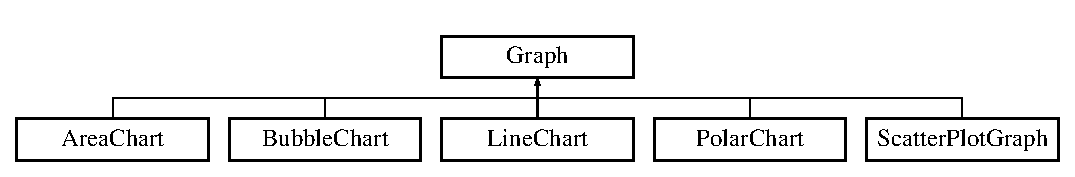
\includegraphics[height=1.931034cm]{interface_graph}
\end{center}
\end{figure}
\subsection*{Public Member Functions}
\begin{DoxyCompactItemize}
\item 
String \hyperlink{interface_graph_a977434fcf3e459b7b2fb643a87f7b17e}{Set\-Label\-X} (String x\-Label)
\item 
String \hyperlink{interface_graph_a0eb8061424e9809e77f33524e2671cfb}{Set\-Label\-Y} (String y\-Label)
\item 
String \hyperlink{interface_graph_a370a17dfe51f613fb29e38572a245095}{Set\-Title} (String graph\-Title)
\end{DoxyCompactItemize}


\subsection{Detailed Description}
An interface for all graph classes. 

\begin{DoxyDate}{Date}
27/02/13 
\end{DoxyDate}
\begin{DoxySeeAlso}{See Also}
\hyperlink{_scatter_plot_graph_8java}{Scatter\-Plot\-Graph.\-java} 
\end{DoxySeeAlso}


\subsection{Member Function Documentation}
\hypertarget{interface_graph_a977434fcf3e459b7b2fb643a87f7b17e}{\index{Graph@{Graph}!Set\-Label\-X@{Set\-Label\-X}}
\index{Set\-Label\-X@{Set\-Label\-X}!Graph@{Graph}}
\subsubsection[{Set\-Label\-X}]{\setlength{\rightskip}{0pt plus 5cm}String Graph.\-Set\-Label\-X (
\begin{DoxyParamCaption}
\item[{String}]{x\-Label}
\end{DoxyParamCaption}
)}}\label{interface_graph_a977434fcf3e459b7b2fb643a87f7b17e}
any class that implements \hyperlink{interface_graph}{Graph} is forced to use the x\-Label variable


\begin{DoxyParams}{Parameters}
{\em x\-Label} & the x axis label passed to the graph by the user \\
\hline
\end{DoxyParams}
\hypertarget{interface_graph_a0eb8061424e9809e77f33524e2671cfb}{\index{Graph@{Graph}!Set\-Label\-Y@{Set\-Label\-Y}}
\index{Set\-Label\-Y@{Set\-Label\-Y}!Graph@{Graph}}
\subsubsection[{Set\-Label\-Y}]{\setlength{\rightskip}{0pt plus 5cm}String Graph.\-Set\-Label\-Y (
\begin{DoxyParamCaption}
\item[{String}]{y\-Label}
\end{DoxyParamCaption}
)}}\label{interface_graph_a0eb8061424e9809e77f33524e2671cfb}
any class that implements \hyperlink{interface_graph}{Graph} is forced to use the y\-Label variable


\begin{DoxyParams}{Parameters}
{\em y\-Label} & the y axis label passed to the graph by the user \\
\hline
\end{DoxyParams}
\hypertarget{interface_graph_a370a17dfe51f613fb29e38572a245095}{\index{Graph@{Graph}!Set\-Title@{Set\-Title}}
\index{Set\-Title@{Set\-Title}!Graph@{Graph}}
\subsubsection[{Set\-Title}]{\setlength{\rightskip}{0pt plus 5cm}String Graph.\-Set\-Title (
\begin{DoxyParamCaption}
\item[{String}]{graph\-Title}
\end{DoxyParamCaption}
)}}\label{interface_graph_a370a17dfe51f613fb29e38572a245095}
any class that implements \hyperlink{interface_graph}{Graph} is forced to use the graph\-Title variable


\begin{DoxyParams}{Parameters}
{\em graph\-Title} & the title passed to the graph by the user \\
\hline
\end{DoxyParams}


The documentation for this class was generated from the following file\-:\begin{DoxyCompactItemize}
\item 
\hyperlink{_graph_8java}{Graph.\-java}\end{DoxyCompactItemize}

\hypertarget{class_group_p_d_m2application}{\section{Group\-P\-D\-M2application Class Reference}
\label{class_group_p_d_m2application}\index{Group\-P\-D\-M2application@{Group\-P\-D\-M2application}}
}


This class creates a new instance of \hyperlink{class_bob_viz}{Bob\-Viz} and parses it to all panels to ensure only one instance of \hyperlink{class_bob_viz}{Bob\-Viz} is ever used.  


\subsection*{Static Public Member Functions}
\begin{DoxyCompactItemize}
\item 
static void \hyperlink{class_group_p_d_m2application_a8f329b12b58123c51f842ed1a80ce1cb}{main} (String\mbox{[}$\,$\mbox{]} args)
\end{DoxyCompactItemize}


\subsection{Detailed Description}
This class creates a new instance of \hyperlink{class_bob_viz}{Bob\-Viz} and parses it to all panels to ensure only one instance of \hyperlink{class_bob_viz}{Bob\-Viz} is ever used. 

\begin{DoxyAuthor}{Author}
Rhys Owen A4, Leopold Stiegler A5, Bradley Coles-\/\-Perkins A6 
\end{DoxyAuthor}
\begin{DoxyDate}{Date}
01/03/2013 
\end{DoxyDate}


\subsection{Member Function Documentation}
\hypertarget{class_group_p_d_m2application_a8f329b12b58123c51f842ed1a80ce1cb}{\index{Group\-P\-D\-M2application@{Group\-P\-D\-M2application}!main@{main}}
\index{main@{main}!GroupPDM2application@{Group\-P\-D\-M2application}}
\subsubsection[{main}]{\setlength{\rightskip}{0pt plus 5cm}static void Group\-P\-D\-M2application.\-main (
\begin{DoxyParamCaption}
\item[{String\mbox{[}$\,$\mbox{]}}]{args}
\end{DoxyParamCaption}
)\hspace{0.3cm}{\ttfamily [static]}}}\label{class_group_p_d_m2application_a8f329b12b58123c51f842ed1a80ce1cb}
This class is used to execute all instances. This makes object programming easier. 
\begin{DoxyParams}{Parameters}
{\em args} & -\/user input not used \\
\hline
\end{DoxyParams}

\begin{DoxyCode}
19                                              \{
20         \textcolor{comment}{/* create new instance of BobViz */}
21         \hyperlink{class_bob_viz}{BobViz} bv = \textcolor{keyword}{new} \hyperlink{class_bob_viz}{BobViz}();
22         
23         \textcolor{comment}{/* send all instances of bv to all classes */}
24         bv.\hyperlink{class_bob_viz_a239767cb7f7f32710826f9efc91b4af9}{GetViz}().\hyperlink{class_visualisation_a8e092a6855febe448999fd1109bc7764}{SetBV}(bv);
25         bv.\hyperlink{class_bob_viz_a93eb7320a1f76d531874cd0bfe5c6b71}{GetImportJPan}().\hyperlink{class_import_j_panel_afea28d8fd4cbe3b480a93a4e7121a41d}{SetBV}(bv);
26         bv.\hyperlink{class_bob_viz_a10dab616869fe644d16c2ccf78627af5}{GetSettingJPan}().\hyperlink{class_setting_j_panel_aabfaa9fb1f2cfc91197b0b5cf10e538d}{SetBV}(bv);
27         bv.\hyperlink{class_bob_viz_aac948a35c1e508b168aad19efba2053d}{GetAboutJPan}().\hyperlink{class_about_j_panel_a134c5a6eee7daba01d35a1ca05ddcca1}{SetBV}(bv);
28         bv.\hyperlink{class_bob_viz_ab8866566b53e78c66e29a4d68406b860}{GetDataset}().\hyperlink{class_dataset_a8de6f8ac02f8378a5510f8014fb2e65f}{SetBV}(bv);
29         bv.\hyperlink{class_bob_viz_a31b771c2acf2b72658beb4f3eecab892}{GetStatusJPan}().\hyperlink{class_status_j_panel_a80d2f3a1eba1516b449115fb8464cfac}{SetBV}(bv);
30         bv.\hyperlink{class_bob_viz_a35af0807f9fca7a0773ce8217b2065c7}{GetVizTypeJPan}().\hyperlink{class_viz_type_j_panel_a83704bbce2513028139d3acea7a85907}{SetBV}(bv);
31         bv.\hyperlink{class_bob_viz_a4b1e563e0fa60594fa0beb1d50438824}{GetGenerateVizJPan}().\hyperlink{class_selection_viz_j_panel_a6287ea60b41d461f06b609340d9c38b4}{SetBV}(bv);
32         
33         bv.\hyperlink{class_bob_viz_a76ae5d60149c159834708456b28d9222}{SetBV}(bv);
34     \}
\end{DoxyCode}


The documentation for this class was generated from the following file\-:\begin{DoxyCompactItemize}
\item 
\hyperlink{_group_p_d_m2application_8java}{Group\-P\-D\-M2application.\-java}\end{DoxyCompactItemize}

\hypertarget{class_import_j_panel}{\section{Import\-J\-Panel Class Reference}
\label{class_import_j_panel}\index{Import\-J\-Panel@{Import\-J\-Panel}}
}


This class provides a import (C\-S\-V file) procedure.  


Inheritance diagram for Import\-J\-Panel\-:\begin{figure}[H]
\begin{center}
\leavevmode
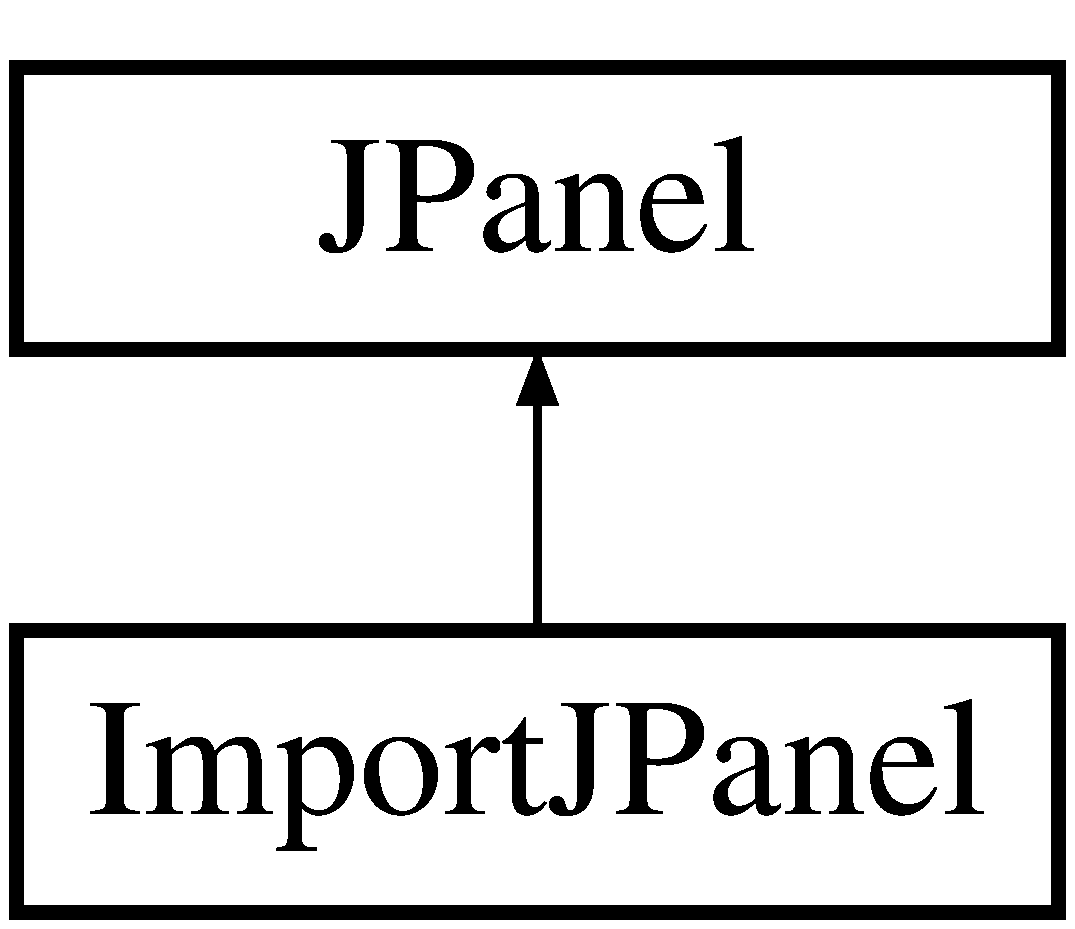
\includegraphics[height=2.000000cm]{class_import_j_panel}
\end{center}
\end{figure}
\subsection*{Public Member Functions}
\begin{DoxyCompactItemize}
\item 
\hyperlink{class_import_j_panel_af9586e0f15e12d4358ee009fcd4192fa}{Import\-J\-Panel} ()
\item 
boolean \hyperlink{class_import_j_panel_aebc2247f219f26a2a4f51d297b82134f}{Set\-Import\-C\-S\-V} ()
\item 
boolean \hyperlink{class_import_j_panel_a2b16a63729e57fdffbcbb42806554929}{Set\-Import\-Second\-C\-S\-V} ()
\item 
boolean \hyperlink{class_import_j_panel_afea28d8fd4cbe3b480a93a4e7121a41d}{Set\-B\-V} (\hyperlink{class_bob_viz}{Bob\-Viz} bv)
\item 
boolean \hyperlink{class_import_j_panel_a9b488ed902bf925d4f48ed5052614f75}{Get\-First\-Check} ()
\item 
boolean \hyperlink{class_import_j_panel_a58a46639a66bbf6ccd78f9a826b7bf81}{Get\-Second\-Check} ()
\end{DoxyCompactItemize}


\subsection{Detailed Description}
This class provides a import (C\-S\-V file) procedure. 

\begin{DoxyDate}{Date}
-\/01/03/2013 
\end{DoxyDate}
\begin{DoxySeeAlso}{See Also}
\hyperlink{_dataset_8java}{Dataset.\-java} 
\end{DoxySeeAlso}


\subsection{Constructor \& Destructor Documentation}
\hypertarget{class_import_j_panel_af9586e0f15e12d4358ee009fcd4192fa}{\index{Import\-J\-Panel@{Import\-J\-Panel}!Import\-J\-Panel@{Import\-J\-Panel}}
\index{Import\-J\-Panel@{Import\-J\-Panel}!ImportJPanel@{Import\-J\-Panel}}
\subsubsection[{Import\-J\-Panel}]{\setlength{\rightskip}{0pt plus 5cm}Import\-J\-Panel.\-Import\-J\-Panel (
\begin{DoxyParamCaption}
{}
\end{DoxyParamCaption}
)}}\label{class_import_j_panel_af9586e0f15e12d4358ee009fcd4192fa}

\begin{DoxyCode}
23                           \{
24         \textcolor{comment}{/* create dimension for ImportJPanel */}
25         Dimension size = getPreferredSize();
26         size.width = WIDTH;
27         size.height = HEIGHT;
28         setPreferredSize( size );
29         
30         setBorder( BorderFactory.createTitledBorder(
31                 BorderFactory.createLineBorder( Color.GRAY ), IMPORT\_CSV
32                 + \textcolor{stringliteral}{"..."} ) );
33         
34         \textcolor{comment}{/* create new import text field for ImportJPanel */}
35         m\_ImportTField = \textcolor{keyword}{new} JTextField( TEXT\_FIELD\_LEN );
36         \textcolor{comment}{/* create new browse button for ImportJPanel */}
37         m\_BrowseJBut = \textcolor{keyword}{new} JButton( BROWSE );
38         
39         \textcolor{comment}{/* create new import text field for ImportJPanel */}
40         m\_ImportSecondTField = \textcolor{keyword}{new} JTextField( TEXT\_FIELD\_LEN );
41         \textcolor{comment}{/* create new browse button for ImportJPanel */}
42         m\_BrowseSecondJBut = \textcolor{keyword}{new} JButton( BROWSE );
43         
44         m\_ImportTField.setEnabled( \textcolor{keyword}{false} );
45         JLabel blank  = \textcolor{keyword}{new} JLabel(\textcolor{stringliteral}{"                                                   "});
46         JLabel about1 = \textcolor{keyword}{new} JLabel(\textcolor{stringliteral}{"<HTML><center>Enter first CSV file:</center></HTML>"});
47         JLabel about2 = \textcolor{keyword}{new} JLabel(\textcolor{stringliteral}{"<HTML><center><p>Enter second CSV file:<br></center>"}
48                         + \textcolor{stringliteral}{"(Leave blank if you wish to visualise one CSV file)</p></HTML>"});
49         
50         \textcolor{comment}{/* add import field and browse button to ImportJPanel */}
51         add( about1 );
52         add( blank );
53         add( m\_ImportTField );
54         add( m\_BrowseJBut );
55         add( about2 );
56         add( m\_ImportSecondTField );
57         add( m\_BrowseSecondJBut );
58         
59         \textcolor{comment}{/* set listeners */}
60         ImportJPanelEventHandler iJEventHandler = \textcolor{keyword}{new} 
61                 ImportJPanelEventHandler();
62         m\_BrowseJBut.addActionListener( iJEventHandler );
63         m\_BrowseSecondJBut.addActionListener( iJEventHandler );
64         m\_BrowseSecondJBut.setEnabled(\textcolor{keyword}{false});  
65     \}    
\end{DoxyCode}


\subsection{Member Function Documentation}
\hypertarget{class_import_j_panel_a9b488ed902bf925d4f48ed5052614f75}{\index{Import\-J\-Panel@{Import\-J\-Panel}!Get\-First\-Check@{Get\-First\-Check}}
\index{Get\-First\-Check@{Get\-First\-Check}!ImportJPanel@{Import\-J\-Panel}}
\subsubsection[{Get\-First\-Check}]{\setlength{\rightskip}{0pt plus 5cm}boolean Import\-J\-Panel.\-Get\-First\-Check (
\begin{DoxyParamCaption}
{}
\end{DoxyParamCaption}
)}}\label{class_import_j_panel_a9b488ed902bf925d4f48ed5052614f75}
Boolean to check if browse button has been selected 
\begin{DoxyCode}
203                                    \{
204         \textcolor{keywordflow}{return} firstCheck;
205     \}
\end{DoxyCode}
\hypertarget{class_import_j_panel_a58a46639a66bbf6ccd78f9a826b7bf81}{\index{Import\-J\-Panel@{Import\-J\-Panel}!Get\-Second\-Check@{Get\-Second\-Check}}
\index{Get\-Second\-Check@{Get\-Second\-Check}!ImportJPanel@{Import\-J\-Panel}}
\subsubsection[{Get\-Second\-Check}]{\setlength{\rightskip}{0pt plus 5cm}boolean Import\-J\-Panel.\-Get\-Second\-Check (
\begin{DoxyParamCaption}
{}
\end{DoxyParamCaption}
)}}\label{class_import_j_panel_a58a46639a66bbf6ccd78f9a826b7bf81}
Boolean to check if second browse button has been selected 
\begin{DoxyCode}
207                                     \{
208         \textcolor{keywordflow}{return} secondCheck;
209     \}
\end{DoxyCode}
\hypertarget{class_import_j_panel_afea28d8fd4cbe3b480a93a4e7121a41d}{\index{Import\-J\-Panel@{Import\-J\-Panel}!Set\-B\-V@{Set\-B\-V}}
\index{Set\-B\-V@{Set\-B\-V}!ImportJPanel@{Import\-J\-Panel}}
\subsubsection[{Set\-B\-V}]{\setlength{\rightskip}{0pt plus 5cm}boolean Import\-J\-Panel.\-Set\-B\-V (
\begin{DoxyParamCaption}
\item[{{\bf Bob\-Viz}}]{bv}
\end{DoxyParamCaption}
)}}\label{class_import_j_panel_afea28d8fd4cbe3b480a93a4e7121a41d}

\begin{DoxyParams}{Parameters}
{\em bv} & -\/ a \hyperlink{class_bob_viz}{Bob\-Viz} object \\
\hline
\end{DoxyParams}
\begin{DoxyReturn}{Returns}
T\-R\-U\-E on success 
\end{DoxyReturn}

\begin{DoxyCode}
190                                       \{
191         \textcolor{keywordtype}{boolean} test = \textcolor{keyword}{true};
192         \textcolor{keywordflow}{if}((test == \textcolor{keyword}{true}) && (bv == null)) \{
193             System.err.println(\textcolor{stringliteral}{"ImportJPanel::SetBV() ***Warning, object"}
194                     + \textcolor{stringliteral}{"is null. Value sent: "} + bv);
195         \} \textcolor{keywordflow}{else} \textcolor{keywordflow}{if} (test == \textcolor{keyword}{true}) \{
196             System.out.println(\textcolor{stringliteral}{"ImportJPanel::SetBV() Object is valid. Value"}
197                     + \textcolor{stringliteral}{"sent: "} + bv);
198         \}
199         m\_BV = bv;
200         \textcolor{keywordflow}{return} \textcolor{keyword}{true};
201     \}
\end{DoxyCode}
\hypertarget{class_import_j_panel_aebc2247f219f26a2a4f51d297b82134f}{\index{Import\-J\-Panel@{Import\-J\-Panel}!Set\-Import\-C\-S\-V@{Set\-Import\-C\-S\-V}}
\index{Set\-Import\-C\-S\-V@{Set\-Import\-C\-S\-V}!ImportJPanel@{Import\-J\-Panel}}
\subsubsection[{Set\-Import\-C\-S\-V}]{\setlength{\rightskip}{0pt plus 5cm}boolean Import\-J\-Panel.\-Set\-Import\-C\-S\-V (
\begin{DoxyParamCaption}
{}
\end{DoxyParamCaption}
)}}\label{class_import_j_panel_aebc2247f219f26a2a4f51d297b82134f}
The method for importing a C\-S\-V file. This method will validate and pass the C\-S\-V file from the G\-U\-I to the dataset class. \begin{DoxyReturn}{Returns}
T\-R\-U\-E if successful 
\end{DoxyReturn}

\begin{DoxyCode}
72                                   \{
73         \textcolor{keywordtype}{boolean} test = \textcolor{keyword}{true};
74         \textcolor{keywordflow}{if}( test == \textcolor{keyword}{true} ) \{
75             updateStatus( WAIT\_FOR\_FILE );
76             \textcolor{comment}{/* set file location */}
77             m\_BV.\hyperlink{class_bob_viz_ab8866566b53e78c66e29a4d68406b860}{GetDataset}().\hyperlink{class_dataset_a26dd0cb28ef8622366d67e21c38b5b0d}{SetFileLocationGUI}();
78             \textcolor{comment}{/* set file location in Dataset */}
79             m\_ImportTField.setText( m\_BV.\hyperlink{class_bob_viz_ab8866566b53e78c66e29a4d68406b860}{GetDataset}().\hyperlink{class_dataset_a91fb1f2a983e9e5bef10864c0f4ec465}{GetFileLocation}() );
80             \textcolor{comment}{/* check for correct file extension */}
81             updateStatus( CHECK\_FILE\_TYPE );
82             \textcolor{comment}{/* check if CSV file */}
83             System.out.println(m\_BV.\hyperlink{class_bob_viz_ab8866566b53e78c66e29a4d68406b860}{GetDataset}().\hyperlink{class_dataset_a01147d9ebdff4ce95ed092143b4c5659}{CheckFileType}());
84             \textcolor{keywordflow}{if}( m\_BV.\hyperlink{class_bob_viz_ab8866566b53e78c66e29a4d68406b860}{GetDataset}().\hyperlink{class_dataset_a01147d9ebdff4ce95ed092143b4c5659}{CheckFileType}() ) \{
85                 updateStatus( ATEMPT\_TO\_READ );
86                 \textcolor{comment}{/* if a CSV file, attempt to read */}
87                 \textcolor{keywordflow}{if}( m\_BV.\hyperlink{class_bob_viz_ab8866566b53e78c66e29a4d68406b860}{GetDataset}().\hyperlink{class_dataset_a54d25635d79320caa77a9d6695e5cf3d}{ReadFile}() ) \{
88                     \textcolor{keywordflow}{if}(m\_BV.\hyperlink{class_bob_viz_ab8866566b53e78c66e29a4d68406b860}{GetDataset}().\hyperlink{class_dataset_a4a0a7e2a2a175ca3d0cebf9431b0e3f4}{GetErrors}() >0)\{
89                         \hyperlink{class_error}{Error} err = \textcolor{keyword}{new} \hyperlink{class_error}{Error}();
90                         \textcolor{keywordflow}{if}(err.\hyperlink{class_error_a56c2216c6ebe6f6b18625d901358ae77}{ReadError}( m\_BV.\hyperlink{class_bob_viz_ab8866566b53e78c66e29a4d68406b860}{GetDataset}().
      \hyperlink{class_dataset_a4a0a7e2a2a175ca3d0cebf9431b0e3f4}{GetErrors}()) == 
91                                 \textcolor{keyword}{true} )\{
92                             m\_BV.\hyperlink{class_bob_viz_ab8866566b53e78c66e29a4d68406b860}{GetDataset}().\hyperlink{class_dataset_abddca267426cbfcbc9a7d250ec53a5e5}{ReadFileBasic}( m\_BV.
      \hyperlink{class_bob_viz_ab8866566b53e78c66e29a4d68406b860}{GetDataset}().
93                                     GetFileLocation() );
94                             
95                         \}
96                             
97                     \}
98                     updateStatus( FILE\_READ\_OK );
99                     m\_BV.\hyperlink{class_bob_viz_a10dab616869fe644d16c2ccf78627af5}{GetSettingJPan}().\hyperlink{class_setting_j_panel_afb2b0736bdf6a8a724066b4a7c78a25f}{SetVizSysType}( m\_BV.
      \hyperlink{class_bob_viz_ab8866566b53e78c66e29a4d68406b860}{GetDataset}().
100                             GetColHeaders() );
101                     \textcolor{comment}{/* enable setting panel components */}
102                     m\_BV.\hyperlink{class_bob_viz_a10dab616869fe644d16c2ccf78627af5}{GetSettingJPan}().\hyperlink{class_setting_j_panel_a0867f721026a690933334532d59fd1c0}{SetSettingsEnabled}( \textcolor{keyword}{true} );
103                     m\_BV.\hyperlink{class_bob_viz_a4b1e563e0fa60594fa0beb1d50438824}{GetGenerateVizJPan}().
      \hyperlink{class_selection_viz_j_panel_ab942f7a1e094e8d3df0df172499c8878}{SetVizJButEnabled}( \textcolor{keyword}{true} );
104                     m\_BV.\hyperlink{class_bob_viz_a4b1e563e0fa60594fa0beb1d50438824}{GetGenerateVizJPan}().
      \hyperlink{class_selection_viz_j_panel_afe28337fc26eb95b02450f6138977c90}{SetSlideshowVizJButEnabled}( \textcolor{keyword}{true} );
105                     m\_BrowseSecondJBut.setEnabled(\textcolor{keyword}{true});
106                     firstCheck = \textcolor{keyword}{true};
107                 \textcolor{comment}{/* if file cannot be read */}
108                 \} \textcolor{keywordflow}{else} \{
109                     
110                 \}
111             \} \textcolor{keywordflow}{else} \{
112                 \textcolor{comment}{/* inform user of wrong file extension */}
113                 JOptionPane.showMessageDialog( null, INVALID\_FILE );
114                 updateStatus( INVALID\_FILE );
115                 m\_BV.\hyperlink{class_bob_viz_a4b1e563e0fa60594fa0beb1d50438824}{GetGenerateVizJPan}().\hyperlink{class_selection_viz_j_panel_ab942f7a1e094e8d3df0df172499c8878}{SetVizJButEnabled}(\textcolor{keyword}{false});
116                 m\_BV.\hyperlink{class_bob_viz_a10dab616869fe644d16c2ccf78627af5}{GetSettingJPan}().\hyperlink{class_setting_j_panel_a0867f721026a690933334532d59fd1c0}{SetSettingsEnabled}(\textcolor{keyword}{false});
117             \}
118         \}
119         \textcolor{keywordflow}{return} \textcolor{keyword}{true};
120     \}
\end{DoxyCode}
\hypertarget{class_import_j_panel_a2b16a63729e57fdffbcbb42806554929}{\index{Import\-J\-Panel@{Import\-J\-Panel}!Set\-Import\-Second\-C\-S\-V@{Set\-Import\-Second\-C\-S\-V}}
\index{Set\-Import\-Second\-C\-S\-V@{Set\-Import\-Second\-C\-S\-V}!ImportJPanel@{Import\-J\-Panel}}
\subsubsection[{Set\-Import\-Second\-C\-S\-V}]{\setlength{\rightskip}{0pt plus 5cm}boolean Import\-J\-Panel.\-Set\-Import\-Second\-C\-S\-V (
\begin{DoxyParamCaption}
{}
\end{DoxyParamCaption}
)}}\label{class_import_j_panel_a2b16a63729e57fdffbcbb42806554929}
The method for importing a second C\-S\-V file. This method will validate and pass the C\-S\-V file from the G\-U\-I to the dataset class. \begin{DoxyReturn}{Returns}
T\-R\-U\-E if successful 
\end{DoxyReturn}

\begin{DoxyCode}
127                                         \{
128         \textcolor{keywordtype}{boolean} test = \textcolor{keyword}{true};
129         \textcolor{keywordflow}{if}( test == \textcolor{keyword}{true} ) \{
130             updateStatus( WAIT\_FOR\_FILE );
131             \textcolor{comment}{/* set file location */}
132             m\_BV.\hyperlink{class_bob_viz_a2826dca37585b5effe3a2f2222f17ada}{GetSecondDataset}().\hyperlink{class_dataset_a26dd0cb28ef8622366d67e21c38b5b0d}{SetFileLocationGUI}();
133             \textcolor{comment}{/* set file location in Dataset */}
134             m\_ImportSecondTField.setText( m\_BV.\hyperlink{class_bob_viz_a2826dca37585b5effe3a2f2222f17ada}{GetSecondDataset}().
      \hyperlink{class_dataset_a91fb1f2a983e9e5bef10864c0f4ec465}{GetFileLocation}() );
135             \textcolor{comment}{/* check for correct file extension */}
136             updateStatus( CHECK\_FILE\_TYPE );
137             \textcolor{comment}{/* check if CSV file */}
138             System.out.println(m\_BV.\hyperlink{class_bob_viz_a2826dca37585b5effe3a2f2222f17ada}{GetSecondDataset}().
      \hyperlink{class_dataset_a01147d9ebdff4ce95ed092143b4c5659}{CheckFileType}());
139             \textcolor{keywordflow}{if}( m\_BV.\hyperlink{class_bob_viz_a2826dca37585b5effe3a2f2222f17ada}{GetSecondDataset}().\hyperlink{class_dataset_a01147d9ebdff4ce95ed092143b4c5659}{CheckFileType}() ) \{
140                 updateStatus( ATEMPT\_TO\_READ );
141                 \textcolor{comment}{/* if a CSV file, attempt to read */}
142                 \textcolor{keywordflow}{if}( m\_BV.\hyperlink{class_bob_viz_a2826dca37585b5effe3a2f2222f17ada}{GetSecondDataset}().\hyperlink{class_dataset_a54d25635d79320caa77a9d6695e5cf3d}{ReadFile}() ) \{
143                     \textcolor{keywordflow}{if}(m\_BV.\hyperlink{class_bob_viz_a2826dca37585b5effe3a2f2222f17ada}{GetSecondDataset}().\hyperlink{class_dataset_a4a0a7e2a2a175ca3d0cebf9431b0e3f4}{GetErrors}() >0)\{
144                         \hyperlink{class_error}{Error} err = \textcolor{keyword}{new} \hyperlink{class_error}{Error}();
145                         \textcolor{keywordflow}{if}(err.\hyperlink{class_error_a56c2216c6ebe6f6b18625d901358ae77}{ReadError}( m\_BV.\hyperlink{class_bob_viz_a2826dca37585b5effe3a2f2222f17ada}{GetSecondDataset}().
      \hyperlink{class_dataset_a4a0a7e2a2a175ca3d0cebf9431b0e3f4}{GetErrors}()) == 
146                                 \textcolor{keyword}{true} )\{
147                             m\_BV.\hyperlink{class_bob_viz_a2826dca37585b5effe3a2f2222f17ada}{GetSecondDataset}().
      \hyperlink{class_dataset_abddca267426cbfcbc9a7d250ec53a5e5}{ReadFileBasic}( m\_BV.\hyperlink{class_bob_viz_a2826dca37585b5effe3a2f2222f17ada}{GetSecondDataset}().
148                                     GetFileLocation() );
149                             
150                         \}
151                             
152                     \}
153                     updateStatus( FILE\_READ\_OK );
154                     m\_BV.\hyperlink{class_bob_viz_a10dab616869fe644d16c2ccf78627af5}{GetSettingJPan}().\hyperlink{class_setting_j_panel_a8c7f693b437db5e8890346d34b68f034}{SetSecondVizSysType}( m\_BV.
      \hyperlink{class_bob_viz_a2826dca37585b5effe3a2f2222f17ada}{GetSecondDataset}().
155                             GetColHeaders() );
156                     \textcolor{comment}{/* enable setting panel components */}
157                     m\_BV.\hyperlink{class_bob_viz_a10dab616869fe644d16c2ccf78627af5}{GetSettingJPan}().\hyperlink{class_setting_j_panel_af44d07f356aa8217418fe0878a50f48d}{SetSecondSettingsEnabled}( \textcolor{keyword}{
      true} );
158                     m\_BV.\hyperlink{class_bob_viz_a4b1e563e0fa60594fa0beb1d50438824}{GetGenerateVizJPan}().
      \hyperlink{class_selection_viz_j_panel_ab942f7a1e094e8d3df0df172499c8878}{SetVizJButEnabled}( \textcolor{keyword}{true} );
159                     m\_BV.\hyperlink{class_bob_viz_a4b1e563e0fa60594fa0beb1d50438824}{GetGenerateVizJPan}().
      \hyperlink{class_selection_viz_j_panel_afe28337fc26eb95b02450f6138977c90}{SetSlideshowVizJButEnabled}( \textcolor{keyword}{true} );
160                     secondCheck = \textcolor{keyword}{true};
161                 \textcolor{comment}{/* if file cannot be read */}
162                 \} \textcolor{keywordflow}{else} \{
163                     
164                 \}
165             \} \textcolor{keywordflow}{else} \{
166                 \textcolor{comment}{/* inform user of wrong file extension */}
167                 JOptionPane.showMessageDialog( null, INVALID\_FILE );
168                 updateStatus( INVALID\_FILE );
169                 m\_BV.\hyperlink{class_bob_viz_a4b1e563e0fa60594fa0beb1d50438824}{GetGenerateVizJPan}().\hyperlink{class_selection_viz_j_panel_ab942f7a1e094e8d3df0df172499c8878}{SetVizJButEnabled}(\textcolor{keyword}{false});
170                 m\_BV.\hyperlink{class_bob_viz_a10dab616869fe644d16c2ccf78627af5}{GetSettingJPan}().\hyperlink{class_setting_j_panel_af44d07f356aa8217418fe0878a50f48d}{SetSecondSettingsEnabled}(\textcolor{keyword}{false})
      ;
171             \}
172         \}
173         \textcolor{keywordflow}{return} \textcolor{keyword}{true};
174     \}
\end{DoxyCode}


The documentation for this class was generated from the following file\-:\begin{DoxyCompactItemize}
\item 
\hyperlink{_import_j_panel_8java}{Import\-J\-Panel.\-java}\end{DoxyCompactItemize}

\hypertarget{class_information_j_panel}{\section{Information\-J\-Panel Class Reference}
\label{class_information_j_panel}\index{Information\-J\-Panel@{Information\-J\-Panel}}
}


A class designed to deal with the Information panel.  


Inheritance diagram for Information\-J\-Panel\-:\begin{figure}[H]
\begin{center}
\leavevmode
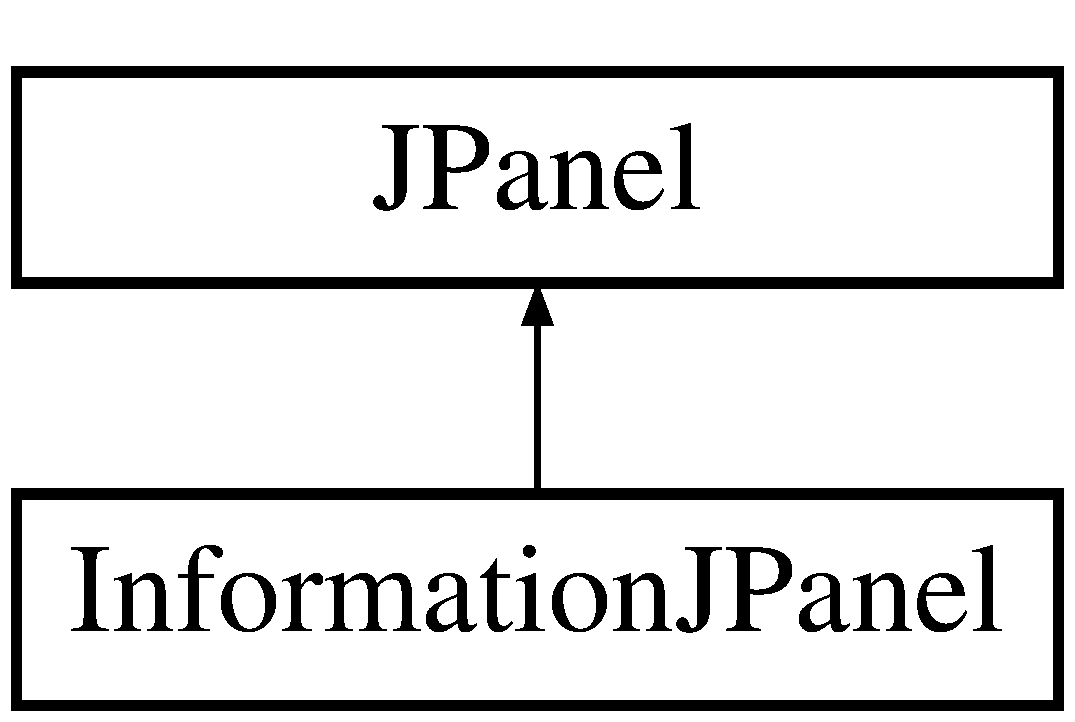
\includegraphics[height=2.000000cm]{class_information_j_panel}
\end{center}
\end{figure}
\subsection*{Public Member Functions}
\begin{DoxyCompactItemize}
\item 
Boolean \hyperlink{class_information_j_panel_a26ab40e4b038442c1d0ad31bb3f5e180}{Set\-Author\-Label} (J\-Label label)
\item 
Boolean \hyperlink{class_information_j_panel_a19b28c461ef20fceb876afa04ef56f3e}{Set\-Author\-Field} (String field)
\item 
Boolean \hyperlink{class_information_j_panel_af098ca9a5d335f46b9b64b5530dfa326}{Set\-Description\-Label} (J\-Label label)
\item 
Boolean \hyperlink{class_information_j_panel_acdc378d528647247674ccf45b071e329}{Set\-Description\-Area} (String area)
\item 
Boolean \hyperlink{class_information_j_panel_ac051ccc3facbbb65afcb8e3246157000}{Set\-Data\-Attribute} (\hyperlink{class_data_attribute}{Data\-Attribute} data)
\item 
J\-Label \hyperlink{class_information_j_panel_a56627ef87297c80e92b05db708a478e2}{Get\-Author\-Label} ()
\item 
J\-Text\-Field \hyperlink{class_information_j_panel_a5a315426cb0994bdcf41713930ffc16c}{Get\-Author\-Field} ()
\item 
J\-Label \hyperlink{class_information_j_panel_a6e2933b638efb56af0c3b7a350222e11}{Get\-Description\-Label} ()
\item 
J\-Text\-Area \hyperlink{class_information_j_panel_a836fd4b83ed476210ba7cbbc10fcf454}{Get\-Description\-Area} ()
\item 
\hyperlink{class_data_attribute}{Data\-Attribute} \hyperlink{class_information_j_panel_aecd081b72d4c75f3a6a92c3edeaf3693}{Get\-Data\-Attribute} ()
\item 
\hyperlink{class_information_j_panel_a78d613b372ae117671a19ee3fffea5f3}{Information\-J\-Panel} (\hyperlink{class_data_attribute}{Data\-Attribute} setting)
\end{DoxyCompactItemize}
\subsection*{Static Public Member Functions}
\begin{DoxyCompactItemize}
\item 
static void \hyperlink{class_information_j_panel_a09618b33446369cf60d4a9eb2035c4f2}{main} (String\mbox{[}$\,$\mbox{]} args)
\end{DoxyCompactItemize}


\subsection{Detailed Description}
A class designed to deal with the Information panel. 

\begin{DoxyAuthor}{Author}
P\-D\-M1 A4
\end{DoxyAuthor}
\begin{DoxyDate}{Date}
14/04/2013 
\end{DoxyDate}


\subsection{Constructor \& Destructor Documentation}
\hypertarget{class_information_j_panel_a78d613b372ae117671a19ee3fffea5f3}{\index{Information\-J\-Panel@{Information\-J\-Panel}!Information\-J\-Panel@{Information\-J\-Panel}}
\index{Information\-J\-Panel@{Information\-J\-Panel}!InformationJPanel@{Information\-J\-Panel}}
\subsubsection[{Information\-J\-Panel}]{\setlength{\rightskip}{0pt plus 5cm}Information\-J\-Panel.\-Information\-J\-Panel (
\begin{DoxyParamCaption}
\item[{{\bf Data\-Attribute}}]{setting}
\end{DoxyParamCaption}
)}}\label{class_information_j_panel_a78d613b372ae117671a19ee3fffea5f3}

\begin{DoxyCode}
106                                                     \{
107         
108         setLayout(\textcolor{keyword}{new} BorderLayout(HGAP,VGAP));
109         TimeStamp ts = \textcolor{keyword}{new} TimeStamp();
110         \hyperlink{class_information_j_panel_ac051ccc3facbbb65afcb8e3246157000}{SetDataAttribute}(setting);
111         \hyperlink{class_information_j_panel_a19b28c461ef20fceb876afa04ef56f3e}{SetAuthorField}(\hyperlink{class_information_j_panel_aecd081b72d4c75f3a6a92c3edeaf3693}{GetDataAttribute}().GetChartAuthor());
112         \hyperlink{class_information_j_panel_acdc378d528647247674ccf45b071e329}{SetDescriptionArea}(\hyperlink{class_information_j_panel_aecd081b72d4c75f3a6a92c3edeaf3693}{GetDataAttribute}().GetChartDescription());
113         \hyperlink{class_information_j_panel_a836fd4b83ed476210ba7cbbc10fcf454}{GetDescriptionArea}().append(\textcolor{stringliteral}{"\(\backslash\)n"} + ts.GetTimeStamp());
114         JScrollPane scrollPane = \textcolor{keyword}{new} JScrollPane(\hyperlink{class_information_j_panel_a836fd4b83ed476210ba7cbbc10fcf454}{GetDescriptionArea}());
115         \hyperlink{class_information_j_panel_a5a315426cb0994bdcf41713930ffc16c}{GetAuthorField}().setEditable(\textcolor{keyword}{false});
116         \hyperlink{class_information_j_panel_a836fd4b83ed476210ba7cbbc10fcf454}{GetDescriptionArea}().setEditable(\textcolor{keyword}{false});
117         \hyperlink{class_information_j_panel_a836fd4b83ed476210ba7cbbc10fcf454}{GetDescriptionArea}().setLineWrap(\textcolor{keyword}{true});
118         \hyperlink{class_information_j_panel_a836fd4b83ed476210ba7cbbc10fcf454}{GetDescriptionArea}().setWrapStyleWord(\textcolor{keyword}{true});
119         
120         JPanel top = \textcolor{keyword}{new} JPanel();
121         JPanel bot = \textcolor{keyword}{new} JPanel();
122         
123         top.add(\hyperlink{class_information_j_panel_a56627ef87297c80e92b05db708a478e2}{GetAuthorLabel}());
124         top.add(\hyperlink{class_information_j_panel_a5a315426cb0994bdcf41713930ffc16c}{GetAuthorField}());
125         bot.add(\hyperlink{class_information_j_panel_a6e2933b638efb56af0c3b7a350222e11}{GetDescriptionLabel}());
126         bot.add(scrollPane);
127         
128         add(top, BorderLayout.CENTER);
129         add(bot, BorderLayout.LINE\_END);
130     \}
\end{DoxyCode}


\subsection{Member Function Documentation}
\hypertarget{class_information_j_panel_a5a315426cb0994bdcf41713930ffc16c}{\index{Information\-J\-Panel@{Information\-J\-Panel}!Get\-Author\-Field@{Get\-Author\-Field}}
\index{Get\-Author\-Field@{Get\-Author\-Field}!InformationJPanel@{Information\-J\-Panel}}
\subsubsection[{Get\-Author\-Field}]{\setlength{\rightskip}{0pt plus 5cm}J\-Text\-Field Information\-J\-Panel.\-Get\-Author\-Field (
\begin{DoxyParamCaption}
{}
\end{DoxyParamCaption}
)}}\label{class_information_j_panel_a5a315426cb0994bdcf41713930ffc16c}
\begin{DoxyReturn}{Returns}
J\-Text\-Field author\-Field 
\end{DoxyReturn}

\begin{DoxyCode}
84                                        \{
85         \textcolor{keywordflow}{return} m\_AuthorField;
86     \}
\end{DoxyCode}
\hypertarget{class_information_j_panel_a56627ef87297c80e92b05db708a478e2}{\index{Information\-J\-Panel@{Information\-J\-Panel}!Get\-Author\-Label@{Get\-Author\-Label}}
\index{Get\-Author\-Label@{Get\-Author\-Label}!InformationJPanel@{Information\-J\-Panel}}
\subsubsection[{Get\-Author\-Label}]{\setlength{\rightskip}{0pt plus 5cm}J\-Label Information\-J\-Panel.\-Get\-Author\-Label (
\begin{DoxyParamCaption}
{}
\end{DoxyParamCaption}
)}}\label{class_information_j_panel_a56627ef87297c80e92b05db708a478e2}
\begin{DoxyReturn}{Returns}
J\-Label author\-Label 
\end{DoxyReturn}

\begin{DoxyCode}
78                                    \{
79         \textcolor{keywordflow}{return} m\_AuthorLabel;
80     \}
\end{DoxyCode}
\hypertarget{class_information_j_panel_aecd081b72d4c75f3a6a92c3edeaf3693}{\index{Information\-J\-Panel@{Information\-J\-Panel}!Get\-Data\-Attribute@{Get\-Data\-Attribute}}
\index{Get\-Data\-Attribute@{Get\-Data\-Attribute}!InformationJPanel@{Information\-J\-Panel}}
\subsubsection[{Get\-Data\-Attribute}]{\setlength{\rightskip}{0pt plus 5cm}{\bf Data\-Attribute} Information\-J\-Panel.\-Get\-Data\-Attribute (
\begin{DoxyParamCaption}
{}
\end{DoxyParamCaption}
)}}\label{class_information_j_panel_aecd081b72d4c75f3a6a92c3edeaf3693}
\begin{DoxyReturn}{Returns}
\hyperlink{class_data_attribute}{Data\-Attribute} data\-Attribute 
\end{DoxyReturn}

\begin{DoxyCode}
102                                             \{
103         \textcolor{keywordflow}{return} m\_DataAttribute;
104     \}
\end{DoxyCode}
\hypertarget{class_information_j_panel_a836fd4b83ed476210ba7cbbc10fcf454}{\index{Information\-J\-Panel@{Information\-J\-Panel}!Get\-Description\-Area@{Get\-Description\-Area}}
\index{Get\-Description\-Area@{Get\-Description\-Area}!InformationJPanel@{Information\-J\-Panel}}
\subsubsection[{Get\-Description\-Area}]{\setlength{\rightskip}{0pt plus 5cm}J\-Text\-Area Information\-J\-Panel.\-Get\-Description\-Area (
\begin{DoxyParamCaption}
{}
\end{DoxyParamCaption}
)}}\label{class_information_j_panel_a836fd4b83ed476210ba7cbbc10fcf454}
\begin{DoxyReturn}{Returns}
J\-Text\-Area description\-Area 
\end{DoxyReturn}

\begin{DoxyCode}
96                                           \{
97         \textcolor{keywordflow}{return} m\_DescriptionField;
98     \}
\end{DoxyCode}
\hypertarget{class_information_j_panel_a6e2933b638efb56af0c3b7a350222e11}{\index{Information\-J\-Panel@{Information\-J\-Panel}!Get\-Description\-Label@{Get\-Description\-Label}}
\index{Get\-Description\-Label@{Get\-Description\-Label}!InformationJPanel@{Information\-J\-Panel}}
\subsubsection[{Get\-Description\-Label}]{\setlength{\rightskip}{0pt plus 5cm}J\-Label Information\-J\-Panel.\-Get\-Description\-Label (
\begin{DoxyParamCaption}
{}
\end{DoxyParamCaption}
)}}\label{class_information_j_panel_a6e2933b638efb56af0c3b7a350222e11}
\begin{DoxyReturn}{Returns}
J\-Label description\-Label 
\end{DoxyReturn}

\begin{DoxyCode}
90                                         \{
91         \textcolor{keywordflow}{return} m\_DescriptionLabel;
92     \}
\end{DoxyCode}
\hypertarget{class_information_j_panel_a09618b33446369cf60d4a9eb2035c4f2}{\index{Information\-J\-Panel@{Information\-J\-Panel}!main@{main}}
\index{main@{main}!InformationJPanel@{Information\-J\-Panel}}
\subsubsection[{main}]{\setlength{\rightskip}{0pt plus 5cm}static void Information\-J\-Panel.\-main (
\begin{DoxyParamCaption}
\item[{String\mbox{[}$\,$\mbox{]}}]{args}
\end{DoxyParamCaption}
)\hspace{0.3cm}{\ttfamily [static]}}}\label{class_information_j_panel_a09618b33446369cf60d4a9eb2035c4f2}

\begin{DoxyCode}
132                                            \{
133         JFrame frame = \textcolor{keyword}{new} JFrame(\textcolor{stringliteral}{"Information Window"});
134         \hyperlink{class_data_attribute}{DataAttribute} data = \textcolor{keyword}{new} \hyperlink{class_data_attribute}{DataAttribute}();
135         TimeStamp timeStamp = \textcolor{keyword}{new} TimeStamp();
136         data.\hyperlink{class_data_attribute_ae2965e7960aaf72643f23a1359daf582}{SetChartAuthor}(\textcolor{stringliteral}{"Author"});
137         data.\hyperlink{class_data_attribute_abbc4a01ce590f81351c3bb527cf18352}{SetChartDesciption}(
138                 \textcolor{stringliteral}{"This is a description of something describable\(\backslash\)n"});
139         frame.add(\textcolor{keyword}{new} \hyperlink{class_information_j_panel_a78d613b372ae117671a19ee3fffea5f3}{InformationJPanel}(data));
140         frame.pack();
141         frame.setVisible(\textcolor{keyword}{true});
142     \}
\end{DoxyCode}
\hypertarget{class_information_j_panel_a19b28c461ef20fceb876afa04ef56f3e}{\index{Information\-J\-Panel@{Information\-J\-Panel}!Set\-Author\-Field@{Set\-Author\-Field}}
\index{Set\-Author\-Field@{Set\-Author\-Field}!InformationJPanel@{Information\-J\-Panel}}
\subsubsection[{Set\-Author\-Field}]{\setlength{\rightskip}{0pt plus 5cm}Boolean Information\-J\-Panel.\-Set\-Author\-Field (
\begin{DoxyParamCaption}
\item[{String}]{field}
\end{DoxyParamCaption}
)}}\label{class_information_j_panel_a19b28c461ef20fceb876afa04ef56f3e}

\begin{DoxyParams}{Parameters}
{\em String} & author\-Field \\
\hline
\end{DoxyParams}
\begin{DoxyReturn}{Returns}
Boolean true -\/ if success 
\end{DoxyReturn}

\begin{DoxyCode}
45                                                 \{ 
46         m\_AuthorField.setText(field);
47         \textcolor{keywordflow}{return} \textcolor{keyword}{true}; 
48     \}
\end{DoxyCode}
\hypertarget{class_information_j_panel_a26ab40e4b038442c1d0ad31bb3f5e180}{\index{Information\-J\-Panel@{Information\-J\-Panel}!Set\-Author\-Label@{Set\-Author\-Label}}
\index{Set\-Author\-Label@{Set\-Author\-Label}!InformationJPanel@{Information\-J\-Panel}}
\subsubsection[{Set\-Author\-Label}]{\setlength{\rightskip}{0pt plus 5cm}Boolean Information\-J\-Panel.\-Set\-Author\-Label (
\begin{DoxyParamCaption}
\item[{J\-Label}]{label}
\end{DoxyParamCaption}
)}}\label{class_information_j_panel_a26ab40e4b038442c1d0ad31bb3f5e180}

\begin{DoxyParams}{Parameters}
{\em J\-Label} & author\-Label \\
\hline
\end{DoxyParams}
\begin{DoxyReturn}{Returns}
Boolean true -\/ if success 
\end{DoxyReturn}

\begin{DoxyCode}
37                                                 \{ 
38         m\_AuthorLabel = label;
39         \textcolor{keywordflow}{return} \textcolor{keyword}{true}; 
40     \}
\end{DoxyCode}
\hypertarget{class_information_j_panel_ac051ccc3facbbb65afcb8e3246157000}{\index{Information\-J\-Panel@{Information\-J\-Panel}!Set\-Data\-Attribute@{Set\-Data\-Attribute}}
\index{Set\-Data\-Attribute@{Set\-Data\-Attribute}!InformationJPanel@{Information\-J\-Panel}}
\subsubsection[{Set\-Data\-Attribute}]{\setlength{\rightskip}{0pt plus 5cm}Boolean Information\-J\-Panel.\-Set\-Data\-Attribute (
\begin{DoxyParamCaption}
\item[{{\bf Data\-Attribute}}]{data}
\end{DoxyParamCaption}
)}}\label{class_information_j_panel_ac051ccc3facbbb65afcb8e3246157000}

\begin{DoxyParams}{Parameters}
{\em \hyperlink{class_data_attribute}{Data\-Attribute}} & data\-Attribute \\
\hline
\end{DoxyParams}
\begin{DoxyReturn}{Returns}
Boolean true -\/ if success 
\end{DoxyReturn}

\begin{DoxyCode}
71                                                         \{
72         m\_DataAttribute = data;
73         \textcolor{keywordflow}{return} \textcolor{keyword}{true};
74     \}
\end{DoxyCode}
\hypertarget{class_information_j_panel_acdc378d528647247674ccf45b071e329}{\index{Information\-J\-Panel@{Information\-J\-Panel}!Set\-Description\-Area@{Set\-Description\-Area}}
\index{Set\-Description\-Area@{Set\-Description\-Area}!InformationJPanel@{Information\-J\-Panel}}
\subsubsection[{Set\-Description\-Area}]{\setlength{\rightskip}{0pt plus 5cm}Boolean Information\-J\-Panel.\-Set\-Description\-Area (
\begin{DoxyParamCaption}
\item[{String}]{area}
\end{DoxyParamCaption}
)}}\label{class_information_j_panel_acdc378d528647247674ccf45b071e329}

\begin{DoxyParams}{Parameters}
{\em String} & description\-Area \\
\hline
\end{DoxyParams}
\begin{DoxyReturn}{Returns}
Boolean true -\/ if success 
\end{DoxyReturn}

\begin{DoxyCode}
63                                                    \{ 
64         m\_DescriptionField.setText(area);
65         \textcolor{keywordflow}{return} \textcolor{keyword}{true}; 
66     \}
\end{DoxyCode}
\hypertarget{class_information_j_panel_af098ca9a5d335f46b9b64b5530dfa326}{\index{Information\-J\-Panel@{Information\-J\-Panel}!Set\-Description\-Label@{Set\-Description\-Label}}
\index{Set\-Description\-Label@{Set\-Description\-Label}!InformationJPanel@{Information\-J\-Panel}}
\subsubsection[{Set\-Description\-Label}]{\setlength{\rightskip}{0pt plus 5cm}Boolean Information\-J\-Panel.\-Set\-Description\-Label (
\begin{DoxyParamCaption}
\item[{J\-Label}]{label}
\end{DoxyParamCaption}
)}}\label{class_information_j_panel_af098ca9a5d335f46b9b64b5530dfa326}

\begin{DoxyParams}{Parameters}
{\em J\-Label} & description\-Label \\
\hline
\end{DoxyParams}
\begin{DoxyReturn}{Returns}
Boolean true -\/ if success 
\end{DoxyReturn}

\begin{DoxyCode}
53                                                      \{ 
54         m\_DescriptionLabel = label;
55         \textcolor{keywordflow}{return} \textcolor{keyword}{true}; 
56     \}
\end{DoxyCode}


The documentation for this class was generated from the following file\-:\begin{DoxyCompactItemize}
\item 
\hyperlink{_information_j_panel_8java}{Information\-J\-Panel.\-java}\end{DoxyCompactItemize}

\hypertarget{class_line_chart}{\section{Line\-Chart Class Reference}
\label{class_line_chart}\index{Line\-Chart@{Line\-Chart}}
}


A class that creates a Line \hyperlink{interface_chart}{Chart} visualisation from a 2\-D Array of data.  


Inheritance diagram for Line\-Chart\-:\begin{figure}[H]
\begin{center}
\leavevmode
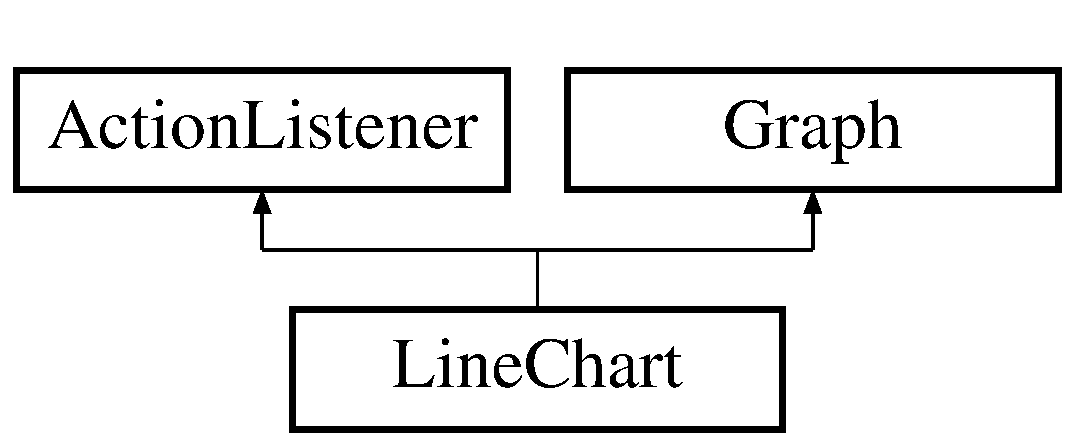
\includegraphics[height=2.000000cm]{class_line_chart}
\end{center}
\end{figure}
\subsection*{Public Member Functions}
\begin{DoxyCompactItemize}
\item 
\hyperlink{class_line_chart_a72fd793f59eb636f6898b73faf9a6a51}{Line\-Chart} (String\mbox{[}$\,$\mbox{]}\mbox{[}$\,$\mbox{]} data, \hyperlink{class_dataset}{Dataset} dataset, \hyperlink{class_data_attribute}{Data\-Attribute} setting)
\item 
\hyperlink{class_line_chart_a23bb447a62c77b3a383022ebeb71671e}{Line\-Chart} (String\mbox{[}$\,$\mbox{]}\mbox{[}$\,$\mbox{]} data, \hyperlink{class_dataset}{Dataset} dataset, \hyperlink{class_data_attribute}{Data\-Attribute} setting, String\mbox{[}$\,$\mbox{]}\mbox{[}$\,$\mbox{]} second\-Data, \hyperlink{class_dataset}{Dataset} second\-Dataset, \hyperlink{class_data_attribute}{Data\-Attribute} second\-Setting)
\item 
\hyperlink{class_line_chart_a4fe8691f64b91f0b18b54696b75e2741}{Line\-Chart} (\hyperlink{class_data_attribute}{Data\-Attribute} setting)
\item 
\hyperlink{class_line_chart_a04d4c60dedbe697b63370bd90414967f}{Line\-Chart} (\hyperlink{class_data_attribute}{Data\-Attribute} setting, \hyperlink{class_data_attribute}{Data\-Attribute} second\-Setting)
\item 
void \hyperlink{class_line_chart_a4c982382761a6da94b9ced6ab33ff171}{action\-Performed} (Action\-Event e)
\item 
String \hyperlink{class_line_chart_a94c65c917dd3d6e0e6e7498f9b68913f}{Set\-Label\-X} (String m\-\_\-x\-Label)
\item 
String \hyperlink{class_line_chart_a64bfe8a0a1a86efad6b5fdaf9ec5d349}{Set\-Seond\-Label\-X} (String m\-\_\-x\-Label)
\item 
String \hyperlink{class_line_chart_ad8947897530ac460222792e166c46880}{Set\-Label\-Y} (String m\-\_\-y\-Label)
\item 
String \hyperlink{class_line_chart_ad3254d9956692f4bddc7ede0951a648d}{Set\-Second\-Label\-Y} (String m\-\_\-y\-Label)
\item 
String \hyperlink{class_line_chart_a22370334f144ff41b288f09aeff798ea}{Set\-Title} (String graph\-Title)
\item 
String \hyperlink{class_line_chart_a27a8002b045b904d09c8d345fb6595a2}{Set\-Second\-Title} (String graph\-Title)
\end{DoxyCompactItemize}
\subsection*{Static Public Member Functions}
\begin{DoxyCompactItemize}
\item 
static void \hyperlink{class_line_chart_aa0459f87c24132d6639b89949bb54022}{main} (String\mbox{[}$\,$\mbox{]} args)
\end{DoxyCompactItemize}


\subsection{Detailed Description}
A class that creates a Line \hyperlink{interface_chart}{Chart} visualisation from a 2\-D Array of data. 

\begin{DoxyDate}{Date}
30/04/13 
\end{DoxyDate}
\begin{DoxySeeAlso}{See Also}

\end{DoxySeeAlso}


\subsection{Constructor \& Destructor Documentation}
\hypertarget{class_line_chart_a72fd793f59eb636f6898b73faf9a6a51}{\index{Line\-Chart@{Line\-Chart}!Line\-Chart@{Line\-Chart}}
\index{Line\-Chart@{Line\-Chart}!LineChart@{Line\-Chart}}
\subsubsection[{Line\-Chart}]{\setlength{\rightskip}{0pt plus 5cm}Line\-Chart.\-Line\-Chart (
\begin{DoxyParamCaption}
\item[{String}]{data\mbox{[}$\,$\mbox{]}\mbox{[}$\,$\mbox{]}, }
\item[{{\bf Dataset}}]{dataset, }
\item[{{\bf Data\-Attribute}}]{setting}
\end{DoxyParamCaption}
)}}\label{class_line_chart_a72fd793f59eb636f6898b73faf9a6a51}
creates a constructor taking in the following parameters\-:


\begin{DoxyParams}{Parameters}
{\em String\mbox{[}$\,$\mbox{]}\mbox{[}$\,$\mbox{]}} & data -\/ data used to create the visualisation. \\
\hline
{\em \hyperlink{class_dataset}{Dataset}} & dataset -\/ the dataset used (rows and columns) \\
\hline
{\em \hyperlink{class_data_attribute}{Data\-Attribute}} & setting -\/ Data attributes \\
\hline
\end{DoxyParams}

\begin{DoxyCode}
43                                                \{
44         
45         m\_Data = data;
46         m\_ChartTitle = setting.\hyperlink{class_data_attribute_ade9747a192ba22fe1020e874bff6a48c}{GetTitle}();
47         m\_Setting = setting;
48         m\_XLabel = setting.\hyperlink{class_data_attribute_aecb451704a87d77dd80dbad8a19099d1}{GetAxisLabelX}();
49         m\_YLabel = setting.\hyperlink{class_data_attribute_af5f68794cd0195d42135d5e48120ccc0}{GetAxisLabelY}();
50         m\_Col = dataset.\hyperlink{class_dataset_ab922bef50c8aa1531de8704731779246}{GetNoOfCols}();
51         m\_Row = dataset.\hyperlink{class_dataset_a91257a605317576e87e1c32e54739e51}{GetNoOfRows}();
52         m\_C1 = setting.\hyperlink{class_data_attribute_a0f4a54973bc44b0526f78bda945dc81b}{GetSelectedXIndex}();
53         m\_C2 = setting.\hyperlink{class_data_attribute_a82e7519853d9f470ea183dd0c39a03d6}{GetSelectedYIndex}();
54         
55         m\_XMin = setting.\hyperlink{class_data_attribute_afa9da883abc4abad5f64c045de114c50}{GetXAxisMin}();
56         m\_XMax = setting.\hyperlink{class_data_attribute_ada370712422c7cbd21b7be4a0d88caf7}{GetXAxisMax}();
57         m\_YMin = setting.\hyperlink{class_data_attribute_af0786b4de674874c0bb8ca9dbe1519c6}{GetYAxisMin}();
58         m\_YMax = setting.\hyperlink{class_data_attribute_a81243eb8f7008e05e74b0f3571d2f08d}{GetYAxisMax}();
59         
60         m\_XScale = setting.\hyperlink{class_data_attribute_a5a1de25600487aa958a19ce01151fea4}{GetXAxisScale}();
61         m\_YScale = setting.\hyperlink{class_data_attribute_a95259727ce91efc0e0eaa28487d944c5}{GetYAxisScale}();
62         
63         createDataset(m\_Data);
64         showChart(m\_Dataset);
65     \}  
\end{DoxyCode}
\hypertarget{class_line_chart_a23bb447a62c77b3a383022ebeb71671e}{\index{Line\-Chart@{Line\-Chart}!Line\-Chart@{Line\-Chart}}
\index{Line\-Chart@{Line\-Chart}!LineChart@{Line\-Chart}}
\subsubsection[{Line\-Chart}]{\setlength{\rightskip}{0pt plus 5cm}Line\-Chart.\-Line\-Chart (
\begin{DoxyParamCaption}
\item[{String}]{data\mbox{[}$\,$\mbox{]}\mbox{[}$\,$\mbox{]}, }
\item[{{\bf Dataset}}]{dataset, }
\item[{{\bf Data\-Attribute}}]{setting, }
\item[{String}]{second\-Data\mbox{[}$\,$\mbox{]}\mbox{[}$\,$\mbox{]}, }
\item[{{\bf Dataset}}]{second\-Dataset, }
\item[{{\bf Data\-Attribute}}]{second\-Setting}
\end{DoxyParamCaption}
)}}\label{class_line_chart_a23bb447a62c77b3a383022ebeb71671e}
creates a constructor taking in the following parameters\-:


\begin{DoxyParams}{Parameters}
{\em String\mbox{[}$\,$\mbox{]}\mbox{[}$\,$\mbox{]}} & data -\/ data used to create the visualisation. \\
\hline
{\em \hyperlink{class_dataset}{Dataset}} & dataset -\/ the dataset used (rows and columns) \\
\hline
{\em \hyperlink{class_data_attribute}{Data\-Attribute}} & setting -\/ Data attributes \\
\hline
{\em String\mbox{[}$\,$\mbox{]}\mbox{[}$\,$\mbox{]}} & second\-Data -\/ second data used to create the visualisation. \\
\hline
{\em \hyperlink{class_dataset}{Dataset}} & second\-Dataset -\/ the second dataset used (rows and columns) \\
\hline
{\em \hyperlink{class_data_attribute}{Data\-Attribute}} & second\-Setting -\/ Second Data attributes \\
\hline
\end{DoxyParams}

\begin{DoxyCode}
78                                          \{
79         
80         m\_Data = data;
81         m\_SecondData = secondData;
82         
83         m\_ChartTitle = setting.\hyperlink{class_data_attribute_ade9747a192ba22fe1020e874bff6a48c}{GetTitle}();
84         m\_SecondChartTitle = secondSetting.\hyperlink{class_data_attribute_a4079522c93025fce7569eaed585f4aeb}{GetSecondTitle}();
85         
86         m\_Setting = setting;
87         m\_SecondSetting = secondSetting;
88         
89         m\_XLabel = setting.\hyperlink{class_data_attribute_aecb451704a87d77dd80dbad8a19099d1}{GetAxisLabelX}();
90         m\_YLabel = setting.\hyperlink{class_data_attribute_af5f68794cd0195d42135d5e48120ccc0}{GetAxisLabelY}();
91         m\_SecondXLabel = secondSetting.\hyperlink{class_data_attribute_a8ace4cb1fee9e2abeabe3efc9a190c8f}{GetSecondAxisLabelX}();
92         m\_SecondYLabel = secondSetting.\hyperlink{class_data_attribute_a6efb7e067317898feefbbf6bd472b998}{GetSecondAxisLabelY}();
93         
94         m\_Col = dataset.\hyperlink{class_dataset_ab922bef50c8aa1531de8704731779246}{GetNoOfCols}();
95         m\_Row = dataset.\hyperlink{class_dataset_a91257a605317576e87e1c32e54739e51}{GetNoOfRows}();
96         m\_SecondCol = secondDataset.\hyperlink{class_dataset_ab922bef50c8aa1531de8704731779246}{GetNoOfCols}();
97         m\_SecondRow = secondDataset.\hyperlink{class_dataset_a91257a605317576e87e1c32e54739e51}{GetNoOfRows}();
98         
99         m\_C1 = setting.\hyperlink{class_data_attribute_a0f4a54973bc44b0526f78bda945dc81b}{GetSelectedXIndex}();
100         m\_C2 = setting.\hyperlink{class_data_attribute_a82e7519853d9f470ea183dd0c39a03d6}{GetSelectedYIndex}();
101 
102         m\_SecondC1 = secondSetting.\hyperlink{class_data_attribute_a7f501790eee650ddf9ac17c4f63a3995}{GetSecondSelectedXIndex}();
103         m\_SecondC2 = secondSetting.\hyperlink{class_data_attribute_a6f61ad05915f4aa31ad3dba00596da64}{GetSecondSelectedYIndex}();
104         
105         m\_XMin = setting.\hyperlink{class_data_attribute_afa9da883abc4abad5f64c045de114c50}{GetXAxisMin}();
106         m\_XMax = setting.\hyperlink{class_data_attribute_ada370712422c7cbd21b7be4a0d88caf7}{GetXAxisMax}();
107         m\_YMin = setting.\hyperlink{class_data_attribute_af0786b4de674874c0bb8ca9dbe1519c6}{GetYAxisMin}();
108         m\_YMax = setting.\hyperlink{class_data_attribute_a81243eb8f7008e05e74b0f3571d2f08d}{GetYAxisMax}();
109         
110         m\_XScale = setting.\hyperlink{class_data_attribute_a5a1de25600487aa958a19ce01151fea4}{GetXAxisScale}();
111         m\_YScale = setting.\hyperlink{class_data_attribute_a95259727ce91efc0e0eaa28487d944c5}{GetYAxisScale}();
112 
113         createDataset(m\_Data);
114         createSecondDataset(m\_SecondData);
115         showChart(m\_Dataset, m\_SecondDataset);
116     \}  
\end{DoxyCode}
\hypertarget{class_line_chart_a4fe8691f64b91f0b18b54696b75e2741}{\index{Line\-Chart@{Line\-Chart}!Line\-Chart@{Line\-Chart}}
\index{Line\-Chart@{Line\-Chart}!LineChart@{Line\-Chart}}
\subsubsection[{Line\-Chart}]{\setlength{\rightskip}{0pt plus 5cm}Line\-Chart.\-Line\-Chart (
\begin{DoxyParamCaption}
\item[{{\bf Data\-Attribute}}]{setting}
\end{DoxyParamCaption}
)}}\label{class_line_chart_a4fe8691f64b91f0b18b54696b75e2741}
constructor for J\-Unit Tests 
\begin{DoxyParams}{Parameters}
{\em setting} & \\
\hline
\end{DoxyParams}

\begin{DoxyCode}
121                                             \{
122         m\_ChartTitle = setting.\hyperlink{class_data_attribute_ade9747a192ba22fe1020e874bff6a48c}{GetTitle}();
123         m\_Setting = setting;
124         m\_XLabel = setting.\hyperlink{class_data_attribute_aecb451704a87d77dd80dbad8a19099d1}{GetAxisLabelX}();
125         m\_YLabel = setting.\hyperlink{class_data_attribute_af5f68794cd0195d42135d5e48120ccc0}{GetAxisLabelY}();
126         m\_C1 = setting.\hyperlink{class_data_attribute_a0f4a54973bc44b0526f78bda945dc81b}{GetSelectedXIndex}();
127         m\_C2 = setting.\hyperlink{class_data_attribute_a82e7519853d9f470ea183dd0c39a03d6}{GetSelectedYIndex}();
128         m\_XMin = setting.\hyperlink{class_data_attribute_afa9da883abc4abad5f64c045de114c50}{GetXAxisMin}();
129         m\_XMax = setting.\hyperlink{class_data_attribute_ada370712422c7cbd21b7be4a0d88caf7}{GetXAxisMax}();
130         m\_YMin = setting.\hyperlink{class_data_attribute_af0786b4de674874c0bb8ca9dbe1519c6}{GetYAxisMin}();
131         m\_YMax = setting.\hyperlink{class_data_attribute_a81243eb8f7008e05e74b0f3571d2f08d}{GetYAxisMax}();
132         m\_XScale = setting.\hyperlink{class_data_attribute_a5a1de25600487aa958a19ce01151fea4}{GetXAxisScale}();
133         m\_YScale = setting.\hyperlink{class_data_attribute_a95259727ce91efc0e0eaa28487d944c5}{GetYAxisScale}();
134     \}
\end{DoxyCode}
\hypertarget{class_line_chart_a04d4c60dedbe697b63370bd90414967f}{\index{Line\-Chart@{Line\-Chart}!Line\-Chart@{Line\-Chart}}
\index{Line\-Chart@{Line\-Chart}!LineChart@{Line\-Chart}}
\subsubsection[{Line\-Chart}]{\setlength{\rightskip}{0pt plus 5cm}Line\-Chart.\-Line\-Chart (
\begin{DoxyParamCaption}
\item[{{\bf Data\-Attribute}}]{setting, }
\item[{{\bf Data\-Attribute}}]{second\-Setting}
\end{DoxyParamCaption}
)}}\label{class_line_chart_a04d4c60dedbe697b63370bd90414967f}
second constructor for J\-Unit Tests 
\begin{DoxyParams}{Parameters}
{\em setting} & \\
\hline
\end{DoxyParams}

\begin{DoxyCode}
139                                                                          \{
140         m\_ChartTitle = setting.\hyperlink{class_data_attribute_ade9747a192ba22fe1020e874bff6a48c}{GetTitle}();
141         m\_Setting = setting;
142         m\_XLabel = setting.\hyperlink{class_data_attribute_aecb451704a87d77dd80dbad8a19099d1}{GetAxisLabelX}();
143         m\_YLabel = setting.\hyperlink{class_data_attribute_af5f68794cd0195d42135d5e48120ccc0}{GetAxisLabelY}();
144         m\_C1 = setting.\hyperlink{class_data_attribute_a0f4a54973bc44b0526f78bda945dc81b}{GetSelectedXIndex}();
145         m\_C2 = setting.\hyperlink{class_data_attribute_a82e7519853d9f470ea183dd0c39a03d6}{GetSelectedYIndex}();
146         m\_XMin = setting.\hyperlink{class_data_attribute_afa9da883abc4abad5f64c045de114c50}{GetXAxisMin}();
147         m\_XMax = setting.\hyperlink{class_data_attribute_ada370712422c7cbd21b7be4a0d88caf7}{GetXAxisMax}();
148         m\_YMin = setting.\hyperlink{class_data_attribute_af0786b4de674874c0bb8ca9dbe1519c6}{GetYAxisMin}();
149         m\_YMax = setting.\hyperlink{class_data_attribute_a81243eb8f7008e05e74b0f3571d2f08d}{GetYAxisMax}();
150         m\_XScale = setting.\hyperlink{class_data_attribute_a5a1de25600487aa958a19ce01151fea4}{GetXAxisScale}();
151         m\_YScale = setting.\hyperlink{class_data_attribute_a95259727ce91efc0e0eaa28487d944c5}{GetYAxisScale}();
152         
153         m\_SecondChartTitle = secondSetting.\hyperlink{class_data_attribute_a4079522c93025fce7569eaed585f4aeb}{GetSecondTitle}();
154         m\_SecondSetting = secondSetting;
155         m\_SecondXLabel = secondSetting.\hyperlink{class_data_attribute_a8ace4cb1fee9e2abeabe3efc9a190c8f}{GetSecondAxisLabelX}();
156         m\_SecondYLabel = secondSetting.\hyperlink{class_data_attribute_a6efb7e067317898feefbbf6bd472b998}{GetSecondAxisLabelY}();
157         m\_SecondC1 = secondSetting.\hyperlink{class_data_attribute_a7f501790eee650ddf9ac17c4f63a3995}{GetSecondSelectedXIndex}();
158         m\_SecondC2 = secondSetting.\hyperlink{class_data_attribute_a6f61ad05915f4aa31ad3dba00596da64}{GetSecondSelectedYIndex}();
159     \}
\end{DoxyCode}


\subsection{Member Function Documentation}
\hypertarget{class_line_chart_a4c982382761a6da94b9ced6ab33ff171}{\index{Line\-Chart@{Line\-Chart}!action\-Performed@{action\-Performed}}
\index{action\-Performed@{action\-Performed}!LineChart@{Line\-Chart}}
\subsubsection[{action\-Performed}]{\setlength{\rightskip}{0pt plus 5cm}void Line\-Chart.\-action\-Performed (
\begin{DoxyParamCaption}
\item[{Action\-Event}]{e}
\end{DoxyParamCaption}
)}}\label{class_line_chart_a4c982382761a6da94b9ced6ab33ff171}
allows user to select the colour of the points on the line chart 
\begin{DoxyCode}
163                                                  \{
164         \textcolor{keywordflow}{if}( e.getSource() == colChangeButton ) \{
165             \hyperlink{class_colour_map}{ColourMap} cM = \textcolor{keyword}{new} \hyperlink{class_colour_map}{ColourMap}();
166             cM.\hyperlink{class_colour_map_a9f696ea699b7fc471bb2dde6f1d1ce09}{SetupData}( m\_Plot.getSeriesCount(), 
167                           m\_Renderer );
168             cM.setVisible( \textcolor{keyword}{false} );
169         \}
170     \}
\end{DoxyCode}
\hypertarget{class_line_chart_aa0459f87c24132d6639b89949bb54022}{\index{Line\-Chart@{Line\-Chart}!main@{main}}
\index{main@{main}!LineChart@{Line\-Chart}}
\subsubsection[{main}]{\setlength{\rightskip}{0pt plus 5cm}static void Line\-Chart.\-main (
\begin{DoxyParamCaption}
\item[{String\mbox{[}$\,$\mbox{]}}]{args}
\end{DoxyParamCaption}
)\hspace{0.3cm}{\ttfamily [static]}}}\label{class_line_chart_aa0459f87c24132d6639b89949bb54022}
main method to carry out J\-Unit Tests 
\begin{DoxyCode}
473                                              \{
474          \textcolor{comment}{// Test to display a single chart}
475         \hyperlink{class_data_attribute}{DataAttribute} test = \hyperlink{class_data_attribute}{DataAttribute}.
      \hyperlink{class_data_attribute_a9c7a1923698c1530fa38c959596199bc}{GetTestDataAttribute}();
476         \hyperlink{class_line_chart}{LineChart} lineChartTest = \textcolor{keyword}{new} \hyperlink{class_line_chart_a72fd793f59eb636f6898b73faf9a6a51}{LineChart}(test);
477         
478         \textcolor{keyword}{final} XYDataset datasetTest = createDataset();
479         lineChartTest.showChart(datasetTest);
480 
481         \textcolor{comment}{// Test to display the two charts}
482         \hyperlink{class_data_attribute}{DataAttribute} secondTest = \hyperlink{class_data_attribute}{DataAttribute}.
      \hyperlink{class_data_attribute_a9c7a1923698c1530fa38c959596199bc}{GetTestDataAttribute}();
483         
484         \hyperlink{class_line_chart}{LineChart} secondLineChartTest = \textcolor{keyword}{new} \hyperlink{class_line_chart_a72fd793f59eb636f6898b73faf9a6a51}{LineChart}(test, secondTest);
485         
486         \textcolor{keyword}{final} XYDataset firstDatasetTest = createDataset();
487         \textcolor{keyword}{final} XYDataset secondDatasetTest = createSecondDataset();
488         
489         secondLineChartTest.showChart(firstDatasetTest,secondDatasetTest);
490         
491     \}
\end{DoxyCode}
\hypertarget{class_line_chart_a94c65c917dd3d6e0e6e7498f9b68913f}{\index{Line\-Chart@{Line\-Chart}!Set\-Label\-X@{Set\-Label\-X}}
\index{Set\-Label\-X@{Set\-Label\-X}!LineChart@{Line\-Chart}}
\subsubsection[{Set\-Label\-X}]{\setlength{\rightskip}{0pt plus 5cm}String Line\-Chart.\-Set\-Label\-X (
\begin{DoxyParamCaption}
\item[{String}]{m\-\_\-x\-Label}
\end{DoxyParamCaption}
)}}\label{class_line_chart_a94c65c917dd3d6e0e6e7498f9b68913f}

\begin{DoxyParams}{Parameters}
{\em m\-\_\-x\-Label} & -\/ the x axis label passed from users to the graph \\
\hline
\end{DoxyParams}
\begin{DoxyReturn}{Returns}
m\-\_\-label\-X -\/ returns the user's x label value 
\end{DoxyReturn}

\begin{DoxyCode}
176                                                \{
177         m\_XLabel = m\_xLabel;
178         \textcolor{keywordflow}{return} m\_XLabel;
179     \}
\end{DoxyCode}
\hypertarget{class_line_chart_ad8947897530ac460222792e166c46880}{\index{Line\-Chart@{Line\-Chart}!Set\-Label\-Y@{Set\-Label\-Y}}
\index{Set\-Label\-Y@{Set\-Label\-Y}!LineChart@{Line\-Chart}}
\subsubsection[{Set\-Label\-Y}]{\setlength{\rightskip}{0pt plus 5cm}String Line\-Chart.\-Set\-Label\-Y (
\begin{DoxyParamCaption}
\item[{String}]{m\-\_\-y\-Label}
\end{DoxyParamCaption}
)}}\label{class_line_chart_ad8947897530ac460222792e166c46880}

\begin{DoxyParams}{Parameters}
{\em m\-\_\-y\-Label} & -\/ the y axis label passed from users to the graph \\
\hline
\end{DoxyParams}
\begin{DoxyReturn}{Returns}
m\-\_\-label\-Y -\/ returns the user's y label value 
\end{DoxyReturn}

\begin{DoxyCode}
194                                                \{
195         String m\_labelY = m\_yLabel;
196         \textcolor{keywordflow}{return} m\_labelY;
197     \}
\end{DoxyCode}
\hypertarget{class_line_chart_ad3254d9956692f4bddc7ede0951a648d}{\index{Line\-Chart@{Line\-Chart}!Set\-Second\-Label\-Y@{Set\-Second\-Label\-Y}}
\index{Set\-Second\-Label\-Y@{Set\-Second\-Label\-Y}!LineChart@{Line\-Chart}}
\subsubsection[{Set\-Second\-Label\-Y}]{\setlength{\rightskip}{0pt plus 5cm}String Line\-Chart.\-Set\-Second\-Label\-Y (
\begin{DoxyParamCaption}
\item[{String}]{m\-\_\-y\-Label}
\end{DoxyParamCaption}
)}}\label{class_line_chart_ad3254d9956692f4bddc7ede0951a648d}

\begin{DoxyParams}{Parameters}
{\em m\-\_\-y\-Label} & -\/ the y axis label passed from users to the graph \\
\hline
\end{DoxyParams}
\begin{DoxyReturn}{Returns}
m\-\_\-\-Second\-Label\-Y -\/ returns the user's second y label value 
\end{DoxyReturn}

\begin{DoxyCode}
202                                                      \{
203         m\_SecondYLabel = m\_yLabel;
204         \textcolor{keywordflow}{return} m\_SecondYLabel;
205     \}
\end{DoxyCode}
\hypertarget{class_line_chart_a27a8002b045b904d09c8d345fb6595a2}{\index{Line\-Chart@{Line\-Chart}!Set\-Second\-Title@{Set\-Second\-Title}}
\index{Set\-Second\-Title@{Set\-Second\-Title}!LineChart@{Line\-Chart}}
\subsubsection[{Set\-Second\-Title}]{\setlength{\rightskip}{0pt plus 5cm}String Line\-Chart.\-Set\-Second\-Title (
\begin{DoxyParamCaption}
\item[{String}]{graph\-Title}
\end{DoxyParamCaption}
)}}\label{class_line_chart_a27a8002b045b904d09c8d345fb6595a2}

\begin{DoxyParams}{Parameters}
{\em String} & graph\-Title -\/ the title passed from users to the graph \\
\hline
\end{DoxyParams}
\begin{DoxyReturn}{Returns}
Second\-Graph\-Title -\/ returns the user's second title value 
\end{DoxyReturn}

\begin{DoxyCode}
219                                                       \{
220         m\_SecondChartTitle = graphTitle;
221         \textcolor{keywordflow}{return} m\_SecondChartTitle;
222     \} 
\end{DoxyCode}
\hypertarget{class_line_chart_a64bfe8a0a1a86efad6b5fdaf9ec5d349}{\index{Line\-Chart@{Line\-Chart}!Set\-Seond\-Label\-X@{Set\-Seond\-Label\-X}}
\index{Set\-Seond\-Label\-X@{Set\-Seond\-Label\-X}!LineChart@{Line\-Chart}}
\subsubsection[{Set\-Seond\-Label\-X}]{\setlength{\rightskip}{0pt plus 5cm}String Line\-Chart.\-Set\-Seond\-Label\-X (
\begin{DoxyParamCaption}
\item[{String}]{m\-\_\-x\-Label}
\end{DoxyParamCaption}
)}}\label{class_line_chart_a64bfe8a0a1a86efad6b5fdaf9ec5d349}

\begin{DoxyParams}{Parameters}
{\em m\-\_\-x\-Label} & -\/ the second x axis label passed from users to the graph \\
\hline
\end{DoxyParams}
\begin{DoxyReturn}{Returns}
m\-\_\-\-Second\-Label\-X -\/ returns the user's second x label value 
\end{DoxyReturn}

\begin{DoxyCode}
185                                                     \{
186         m\_SecondXLabel = m\_xLabel;
187         \textcolor{keywordflow}{return} m\_SecondXLabel;
188     \}
\end{DoxyCode}
\hypertarget{class_line_chart_a22370334f144ff41b288f09aeff798ea}{\index{Line\-Chart@{Line\-Chart}!Set\-Title@{Set\-Title}}
\index{Set\-Title@{Set\-Title}!LineChart@{Line\-Chart}}
\subsubsection[{Set\-Title}]{\setlength{\rightskip}{0pt plus 5cm}String Line\-Chart.\-Set\-Title (
\begin{DoxyParamCaption}
\item[{String}]{graph\-Title}
\end{DoxyParamCaption}
)}}\label{class_line_chart_a22370334f144ff41b288f09aeff798ea}

\begin{DoxyParams}{Parameters}
{\em String} & graph\-Title -\/ the title passed from users to the graph \\
\hline
\end{DoxyParams}
\begin{DoxyReturn}{Returns}
graph\-Title -\/ returns the user's title value 
\end{DoxyReturn}

\begin{DoxyCode}
211                                                 \{
212         String m\_title = graphTitle;
213         \textcolor{keywordflow}{return} m\_title;
214     \} 
\end{DoxyCode}


The documentation for this class was generated from the following file\-:\begin{DoxyCompactItemize}
\item 
\hyperlink{_line_chart_8java}{Line\-Chart.\-java}\end{DoxyCompactItemize}

\hypertarget{class_more_setting_j_panel}{\section{More\-Setting\-J\-Panel Class Reference}
\label{class_more_setting_j_panel}\index{More\-Setting\-J\-Panel@{More\-Setting\-J\-Panel}}
}


A class designed to deal with the 'More Settings' panel.  


Inheritance diagram for More\-Setting\-J\-Panel\-:\begin{figure}[H]
\begin{center}
\leavevmode
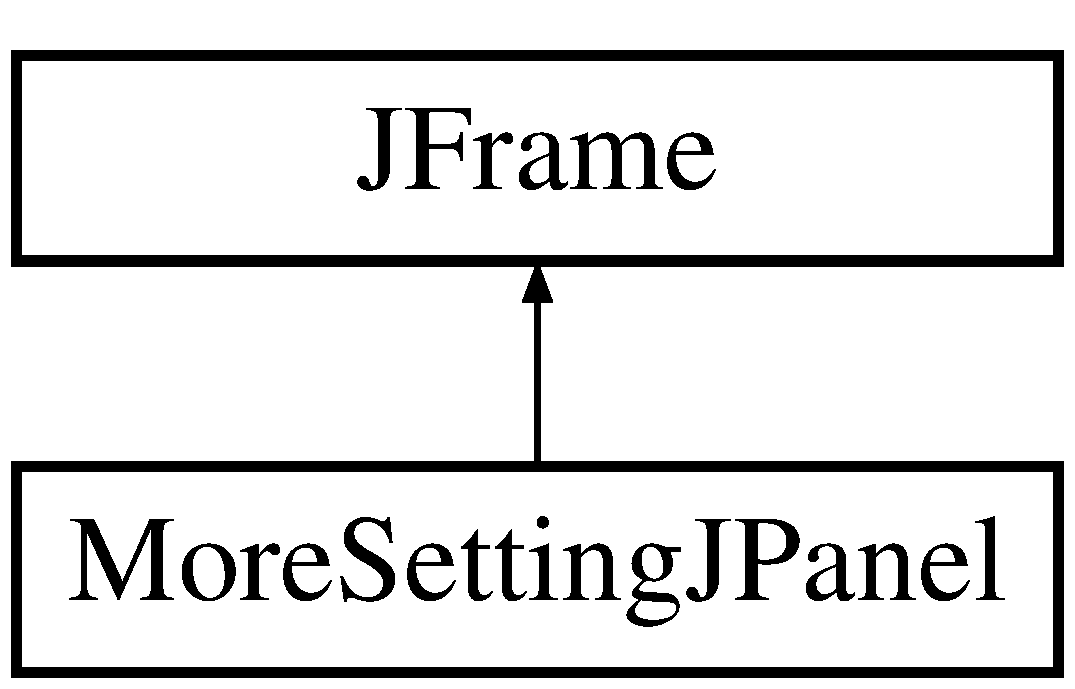
\includegraphics[height=2.000000cm]{class_more_setting_j_panel}
\end{center}
\end{figure}
\subsection*{Public Member Functions}
\begin{DoxyCompactItemize}
\item 
J\-Text\-Field \hyperlink{class_more_setting_j_panel_a55adb7a6be529276552eb98cb3c76fd0}{Get\-X\-Axis\-Min\-Field} ()
\item 
J\-Text\-Field \hyperlink{class_more_setting_j_panel_ae412bd3a66df2b14af9aae95c6ee55d8}{Get\-X\-Axis\-Max\-Field} ()
\item 
J\-Text\-Field \hyperlink{class_more_setting_j_panel_a451f95a3e1c0231aded2bf8fa3b4421d}{Get\-Y\-Axis\-Min\-Field} ()
\item 
J\-Text\-Field \hyperlink{class_more_setting_j_panel_ab524a65ef89a39d61e7033e7495a53c4}{Get\-Y\-Axis\-Max\-Field} ()
\item 
J\-Text\-Field \hyperlink{class_more_setting_j_panel_ab091eb7f112297574ccd612011b91e73}{Get\-X\-Axis\-Scale\-Field} ()
\item 
J\-Text\-Field \hyperlink{class_more_setting_j_panel_a13bfe944b0b4a671dc37c1c87381024d}{Get\-Y\-Axis\-Scale\-Field} ()
\item 
J\-Toggle\-Button \hyperlink{class_more_setting_j_panel_ab1f181103d7e162919eb257a3b0d04ca}{Get\-Default\-Button} ()
\item 
double \hyperlink{class_more_setting_j_panel_a497d4195007c03bfd6dbf909904f001d}{Get\-X\-Axis\-Min} ()
\item 
double \hyperlink{class_more_setting_j_panel_a2de92046bd03e4d6173acf6528439f53}{Get\-X\-Axis\-Max} ()
\item 
double \hyperlink{class_more_setting_j_panel_a81ac83574297de3b0cce60b91af661ef}{Get\-Y\-Axis\-Min} ()
\item 
double \hyperlink{class_more_setting_j_panel_a3d22ee97ad0adefd68746ac67630861f}{Get\-Y\-Axis\-Max} ()
\item 
double \hyperlink{class_more_setting_j_panel_afb3b2d456021f75e7d5ca438da32c5ad}{Get\-X\-Axis\-Scale} ()
\item 
double \hyperlink{class_more_setting_j_panel_ae137e83634e54fdca50c6cfeff6e451e}{Get\-Y\-Axis\-Scale} ()
\item 
String \hyperlink{class_more_setting_j_panel_a3940f844aa7de03b4607a3ce010eaa1f}{Get\-Author} ()
\item 
String \hyperlink{class_more_setting_j_panel_a02e5419e3a676912f28da9c6bbebc464}{Get\-Description} ()
\item 
\hyperlink{class_more_setting_j_panel_ac87617b1baff19cf09ecf2d713b4b368}{More\-Setting\-J\-Panel} (\hyperlink{class_data_attribute}{Data\-Attribute} chart\-Setting)
\end{DoxyCompactItemize}
\subsection*{Static Public Member Functions}
\begin{DoxyCompactItemize}
\item 
static void \hyperlink{class_more_setting_j_panel_a313c7e51f47e39c3cb424850e044708c}{main} (String\mbox{[}$\,$\mbox{]} args)
\end{DoxyCompactItemize}
\subsection*{Public Attributes}
\begin{DoxyCompactItemize}
\item 
final int \hyperlink{class_more_setting_j_panel_a09bffa47a9133c9966cf18961bf3a46e}{F\-R\-A\-M\-E\-\_\-\-W\-I\-D\-T\-H} = 500
\item 
final int \hyperlink{class_more_setting_j_panel_affa56095abc301bb764a5711fd097ac8}{F\-R\-A\-M\-E\-\_\-\-H\-E\-I\-G\-H\-T} = 200
\end{DoxyCompactItemize}


\subsection{Detailed Description}
A class designed to deal with the 'More Settings' panel. 

\begin{DoxyAuthor}{Author}
P\-D\-M1 A4
\end{DoxyAuthor}
\begin{DoxyDate}{Date}
14/04/2013 
\end{DoxyDate}


\subsection{Constructor \& Destructor Documentation}
\hypertarget{class_more_setting_j_panel_ac87617b1baff19cf09ecf2d713b4b368}{\index{More\-Setting\-J\-Panel@{More\-Setting\-J\-Panel}!More\-Setting\-J\-Panel@{More\-Setting\-J\-Panel}}
\index{More\-Setting\-J\-Panel@{More\-Setting\-J\-Panel}!MoreSettingJPanel@{More\-Setting\-J\-Panel}}
\subsubsection[{More\-Setting\-J\-Panel}]{\setlength{\rightskip}{0pt plus 5cm}More\-Setting\-J\-Panel.\-More\-Setting\-J\-Panel (
\begin{DoxyParamCaption}
\item[{{\bf Data\-Attribute}}]{chart\-Setting}
\end{DoxyParamCaption}
)}}\label{class_more_setting_j_panel_ac87617b1baff19cf09ecf2d713b4b368}

\begin{DoxyCode}
218                                                          \{
219         super(\textcolor{stringliteral}{"Additional settings"});
220         m\_ChartSetting = chartSetting;
221         
222         setSize(\textcolor{keyword}{new} Dimension(\hyperlink{class_more_setting_j_panel_a09bffa47a9133c9966cf18961bf3a46e}{FRAME\_WIDTH},\hyperlink{class_more_setting_j_panel_affa56095abc301bb764a5711fd097ac8}{FRAME\_HEIGHT}));
223         
224         m\_MainPanel = \textcolor{keyword}{new} JPanel();
225         
226         m\_XAxisMinLabel = \textcolor{keyword}{new} JLabel();
227         m\_XAxisMaxLabel = \textcolor{keyword}{new} JLabel();
228         m\_XAxisMinField = \textcolor{keyword}{new} JTextField(NUMBER\_FIELD\_LEN);
229         m\_XAxisMaxField = \textcolor{keyword}{new} JTextField(NUMBER\_FIELD\_LEN);
230         m\_XAxisMinField.setText(String.valueOf(m\_ChartSetting.\hyperlink{class_data_attribute_afa9da883abc4abad5f64c045de114c50}{GetXAxisMin}()));
231         m\_XAxisMaxField.setText(String.valueOf(m\_ChartSetting.\hyperlink{class_data_attribute_ada370712422c7cbd21b7be4a0d88caf7}{GetXAxisMax}()));
232         
233         m\_YAxisMinLabel = \textcolor{keyword}{new} JLabel();
234         m\_YAxisMaxLabel = \textcolor{keyword}{new} JLabel();
235         m\_YAxisMinField = \textcolor{keyword}{new} JTextField(NUMBER\_FIELD\_LEN);
236         m\_YAxisMaxField = \textcolor{keyword}{new} JTextField(NUMBER\_FIELD\_LEN);
237         m\_YAxisMinField.setText(String.valueOf(m\_ChartSetting.\hyperlink{class_data_attribute_af0786b4de674874c0bb8ca9dbe1519c6}{GetYAxisMin}()));
238         m\_YAxisMaxField.setText(String.valueOf(m\_ChartSetting.\hyperlink{class_data_attribute_a81243eb8f7008e05e74b0f3571d2f08d}{GetYAxisMax}()));
239         
240         m\_XAxisScaleLabel = \textcolor{keyword}{new} JLabel();
241         m\_YAxisScaleLabel = \textcolor{keyword}{new} JLabel();
242         m\_XAxisScaleField = \textcolor{keyword}{new} JTextField(NUMBER\_FIELD\_LEN);
243         m\_YAxisScaleField = \textcolor{keyword}{new} JTextField(NUMBER\_FIELD\_LEN);
244         m\_XAxisScaleField.setText(
245                 String.valueOf(m\_ChartSetting.\hyperlink{class_data_attribute_a5a1de25600487aa958a19ce01151fea4}{GetXAxisScale}()));
246         m\_YAxisScaleField.setText(
247                 String.valueOf(m\_ChartSetting.\hyperlink{class_data_attribute_a95259727ce91efc0e0eaa28487d944c5}{GetYAxisScale}()));
248         
249         m\_AuthorLabel = \textcolor{keyword}{new} JLabel();
250         m\_AuthorField = \textcolor{keyword}{new} JTextField(TEXT\_FIELD\_LEN);
251         m\_DesciptionLabel = \textcolor{keyword}{new} JLabel();
252         
253         m\_DescriptionField = \textcolor{keyword}{new} JTextArea();
254         m\_DescriptionField.setLineWrap(\textcolor{keyword}{true});
255         m\_DescriptionField.setWrapStyleWord(\textcolor{keyword}{true});
256         
257         m\_ApplyButton = \textcolor{keyword}{new} JButton();
258         m\_DefaultButton = \textcolor{keyword}{new} JToggleButton();
259         m\_DefaultButton.setSelected(\textcolor{keyword}{true});
260 
261         m\_XAxisMinLabel.setText(\textcolor{stringliteral}{"X min: "});
262         m\_XAxisMaxLabel.setText(\textcolor{stringliteral}{"X max:"});
263         m\_YAxisMinLabel.setText(\textcolor{stringliteral}{"Y min: "});
264         m\_YAxisMaxLabel.setText(\textcolor{stringliteral}{"Y max:"});
265 
266         m\_XAxisScaleLabel.setText(\textcolor{stringliteral}{"X scale:"});
267         m\_YAxisScaleLabel.setText(\textcolor{stringliteral}{"Y scale:"});
268         m\_AuthorLabel.setText(\textcolor{stringliteral}{"Author:"});
269         m\_DesciptionLabel.setText(\textcolor{stringliteral}{"Description:"});
270 
271         m\_ApplyButton.setText(\textcolor{stringliteral}{"Apply"});
272         m\_DefaultButton.setText(\textcolor{stringliteral}{"Default"});
273         
274         SettingJPanelEventHandler handler = \textcolor{keyword}{new} SettingJPanelEventHandler();
275         m\_ApplyButton.addActionListener(handler);
276         m\_DefaultButton.addActionListener(handler);
277         
278 
279         javax.swing.GroupLayout layout = \textcolor{keyword}{new} GroupLayout(m\_MainPanel);
280         m\_MainPanel.setLayout(layout);
281         layout.setHorizontalGroup(
282             layout.createParallelGroup(GroupLayout.Alignment.LEADING)
283             .addGroup(layout.createSequentialGroup()
284                 .addContainerGap()
285                 .addGroup(layout.createParallelGroup(
286                         GroupLayout.Alignment.LEADING)
287                     .addGroup(layout.createSequentialGroup()
288                         .addGroup(layout.createParallelGroup(
289                                 GroupLayout.Alignment.LEADING)
290                             .addGroup(layout.createSequentialGroup()
291                                 .addComponent(m\_XAxisScaleLabel)
292                                 .addPreferredGap(LayoutStyle.
293                                         ComponentPlacement.UNRELATED)
294                                 .addComponent(m\_XAxisScaleField, 
295                                         GroupLayout.PREFERRED\_SIZE, 
296                                         GroupLayout.DEFAULT\_SIZE, 
297                                         GroupLayout.PREFERRED\_SIZE)
298                                 .addGap(GAP\_1, GAP\_1, GAP\_1)
299                                 .addComponent(m\_AuthorLabel))
300                             .addGroup(layout.createSequentialGroup()
301                                 .addComponent(m\_YAxisScaleLabel)
302                                 .addPreferredGap(LayoutStyle
303                                         .ComponentPlacement.UNRELATED)
304                                 .addComponent(m\_YAxisScaleField, 
305                                         GroupLayout.PREFERRED\_SIZE, 
306                                         GroupLayout.DEFAULT\_SIZE, 
307                                         GroupLayout.PREFERRED\_SIZE)))
308                         .addPreferredGap(LayoutStyle
309                                 .ComponentPlacement.RELATED,
310                                 GroupLayout.DEFAULT\_SIZE, Short.MAX\_VALUE)
311                         .addComponent(m\_AuthorField, 
312                                 GroupLayout.PREFERRED\_SIZE, 
313                                 GroupLayout.DEFAULT\_SIZE, 
314                                 GroupLayout.PREFERRED\_SIZE))
315                     .addGroup(layout.createSequentialGroup()
316                         .addGroup(layout.createParallelGroup(
317                                 GroupLayout.Alignment.LEADING)
318                             .addGroup(layout.createSequentialGroup()
319                                 .addComponent(m\_XAxisMinLabel)
320                                 .addPreferredGap(LayoutStyle
321                                         .ComponentPlacement.UNRELATED)
322                                 .addComponent(m\_XAxisMinField,
323                                         GroupLayout.PREFERRED\_SIZE, 
324                                         GroupLayout.DEFAULT\_SIZE, 
325                                         GroupLayout.PREFERRED\_SIZE)
326                                 .addGap(GAP\_1, GAP\_1, GAP\_1)
327                                 .addComponent(m\_YAxisMinLabel)
328                                 .addPreferredGap(LayoutStyle
329                                         .ComponentPlacement.UNRELATED)
330                                 .addComponent(m\_YAxisMinField, 
331                                         GroupLayout.PREFERRED\_SIZE, 
332                                         GroupLayout.DEFAULT\_SIZE, 
333                                         GroupLayout.PREFERRED\_SIZE))
334                             .addGroup(layout.createSequentialGroup()
335                                 .addComponent(m\_XAxisMaxLabel)
336                                 .addPreferredGap(LayoutStyle
337                                         .ComponentPlacement.UNRELATED)
338                                 .addComponent(m\_XAxisMaxField, 
339                                         GroupLayout.PREFERRED\_SIZE, 
340                                         GroupLayout.DEFAULT\_SIZE, 
341                                         GroupLayout.PREFERRED\_SIZE)
342                                 .addGap(GAP\_1, GAP\_1, GAP\_1)
343                                 .addComponent(m\_YAxisMaxLabel)
344                                 .addPreferredGap(LayoutStyle
345                                         .ComponentPlacement.UNRELATED)
346                                 .addComponent(m\_YAxisMaxField, 
347                                         GroupLayout.PREFERRED\_SIZE,
348                                         GroupLayout.DEFAULT\_SIZE, 
349                                         GroupLayout.PREFERRED\_SIZE)))
350                         .addGap(0, 0, Short.MAX\_VALUE))
351                     .addGroup(layout.createSequentialGroup()
352                         .addComponent(m\_DesciptionLabel)
353                         .addPreferredGap(LayoutStyle
354                                 .ComponentPlacement.UNRELATED)
355                         .addComponent(m\_DescriptionField))
356                     .addGroup(GroupLayout.Alignment.TRAILING, 
357                               layout.createSequentialGroup()
358                         .addGap(0, 0, Short.MAX\_VALUE)
359                         .addPreferredGap(LayoutStyle
360                                 .ComponentPlacement.RELATED)
361                         .addComponent(m\_DefaultButton)
362                         .addComponent(m\_ApplyButton)))
363                 .addContainerGap())
364         );
365         layout.setVerticalGroup(
366             layout.createParallelGroup(GroupLayout.Alignment.LEADING)
367             .addGroup(layout.createSequentialGroup()
368                 .addContainerGap()
369                 .addGroup(layout.createParallelGroup(
370                         GroupLayout.Alignment.BASELINE)
371                     .addComponent(m\_XAxisMinLabel)
372                     .addComponent(m\_XAxisMinField, 
373                             GroupLayout.PREFERRED\_SIZE, 
374                             GroupLayout.DEFAULT\_SIZE, 
375                             GroupLayout.PREFERRED\_SIZE)
376                     .addComponent(m\_YAxisMinLabel)
377                     .addComponent(m\_YAxisMinField, 
378                             GroupLayout.PREFERRED\_SIZE, 
379                             GroupLayout.DEFAULT\_SIZE, 
380                             GroupLayout.PREFERRED\_SIZE))
381                 .addPreferredGap(LayoutStyle.ComponentPlacement.RELATED)
382                 .addGroup(layout.createParallelGroup(
383                         GroupLayout.Alignment.BASELINE)
384                     .addComponent(m\_XAxisMaxLabel)
385                     .addComponent(m\_XAxisMaxField, 
386                             GroupLayout.PREFERRED\_SIZE, 
387                             GroupLayout.DEFAULT\_SIZE, 
388                             GroupLayout.PREFERRED\_SIZE)
389                     .addComponent(m\_YAxisMaxLabel)
390                     .addComponent(m\_YAxisMaxField, 
391                             GroupLayout.PREFERRED\_SIZE, 
392                             GroupLayout.DEFAULT\_SIZE,
393                             GroupLayout.PREFERRED\_SIZE))
394                 .addGroup(layout.createParallelGroup(
395                         GroupLayout.Alignment.LEADING)
396                     .addGroup(layout.createSequentialGroup()
397                         .addGap(GAP\_1, GAP\_1, GAP\_1)
398                         .addGroup(layout.createParallelGroup(
399                                 GroupLayout.Alignment.BASELINE)
400                             .addComponent(m\_XAxisScaleLabel)
401                             .addComponent(m\_XAxisScaleField, 
402                                     GroupLayout.PREFERRED\_SIZE, 
403                                     GroupLayout.DEFAULT\_SIZE, 
404                                     GroupLayout.PREFERRED\_SIZE))
405                         .addPreferredGap(LayoutStyle
406                                 .ComponentPlacement.RELATED)
407                         .addGroup(layout.createParallelGroup(
408                                 GroupLayout.Alignment.BASELINE)
409                             .addComponent(m\_YAxisScaleLabel)
410                             .addComponent(m\_YAxisScaleField, 
411                                     GroupLayout.PREFERRED\_SIZE, 
412                                     GroupLayout.DEFAULT\_SIZE, 
413                                     GroupLayout.PREFERRED\_SIZE)))
414                     .addGroup(layout.createSequentialGroup()
415                         .addGap(GAP\_2, GAP\_2, GAP\_2)
416                         .addGroup(layout.createParallelGroup(
417                                 GroupLayout.Alignment.BASELINE)
418                             .addComponent(m\_AuthorLabel)
419                             .addComponent(m\_AuthorField, 
420                                     GroupLayout.PREFERRED\_SIZE, 
421                                     GroupLayout.DEFAULT\_SIZE, 
422                                     GroupLayout.PREFERRED\_SIZE))))
423                 .addGap(GAP\_1, GAP\_1, GAP\_1)
424                 .addGroup(layout.createParallelGroup(
425                         GroupLayout.Alignment.BASELINE)
426                     .addComponent(m\_DesciptionLabel)
427                     .addComponent(m\_DescriptionField, 
428                             GroupLayout.PREFERRED\_SIZE, SIZE,
429                             GroupLayout.PREFERRED\_SIZE))
430                 .addPreferredGap(LayoutStyle.ComponentPlacement.UNRELATED)
431                 .addGroup(layout.createParallelGroup(
432                         GroupLayout.Alignment.BASELINE)
433                     .addComponent(m\_ApplyButton)
434                     .addComponent(m\_DefaultButton))
435                 .addContainerGap(GroupLayout.DEFAULT\_SIZE, Short.MAX\_VALUE))
436         );
437         
438         add(m\_MainPanel);
439         setDefaultCloseOperation(JFrame.DISPOSE\_ON\_CLOSE);
440         pack();
441     \}
\end{DoxyCode}


\subsection{Member Function Documentation}
\hypertarget{class_more_setting_j_panel_a3940f844aa7de03b4607a3ce010eaa1f}{\index{More\-Setting\-J\-Panel@{More\-Setting\-J\-Panel}!Get\-Author@{Get\-Author}}
\index{Get\-Author@{Get\-Author}!MoreSettingJPanel@{More\-Setting\-J\-Panel}}
\subsubsection[{Get\-Author}]{\setlength{\rightskip}{0pt plus 5cm}String More\-Setting\-J\-Panel.\-Get\-Author (
\begin{DoxyParamCaption}
{}
\end{DoxyParamCaption}
)}}\label{class_more_setting_j_panel_a3940f844aa7de03b4607a3ce010eaa1f}
Gets Authour Text

\begin{DoxyReturn}{Returns}
Author Field 
\end{DoxyReturn}

\begin{DoxyCode}
200                               \{
201         \textcolor{keywordflow}{return} m\_AuthorField.getText();
202     \}
\end{DoxyCode}
\hypertarget{class_more_setting_j_panel_ab1f181103d7e162919eb257a3b0d04ca}{\index{More\-Setting\-J\-Panel@{More\-Setting\-J\-Panel}!Get\-Default\-Button@{Get\-Default\-Button}}
\index{Get\-Default\-Button@{Get\-Default\-Button}!MoreSettingJPanel@{More\-Setting\-J\-Panel}}
\subsubsection[{Get\-Default\-Button}]{\setlength{\rightskip}{0pt plus 5cm}J\-Toggle\-Button More\-Setting\-J\-Panel.\-Get\-Default\-Button (
\begin{DoxyParamCaption}
{}
\end{DoxyParamCaption}
)}}\label{class_more_setting_j_panel_ab1f181103d7e162919eb257a3b0d04ca}
Gets Default Button

\begin{DoxyReturn}{Returns}
Default Button 
\end{DoxyReturn}

\begin{DoxyCode}
112                                             \{
113         \textcolor{keywordflow}{return} m\_DefaultButton;
114     \}
\end{DoxyCode}
\hypertarget{class_more_setting_j_panel_a02e5419e3a676912f28da9c6bbebc464}{\index{More\-Setting\-J\-Panel@{More\-Setting\-J\-Panel}!Get\-Description@{Get\-Description}}
\index{Get\-Description@{Get\-Description}!MoreSettingJPanel@{More\-Setting\-J\-Panel}}
\subsubsection[{Get\-Description}]{\setlength{\rightskip}{0pt plus 5cm}String More\-Setting\-J\-Panel.\-Get\-Description (
\begin{DoxyParamCaption}
{}
\end{DoxyParamCaption}
)}}\label{class_more_setting_j_panel_a02e5419e3a676912f28da9c6bbebc464}
Gets Description Text

\begin{DoxyReturn}{Returns}
Description Text Field 
\end{DoxyReturn}

\begin{DoxyCode}
208                                    \{
209         \textcolor{keywordflow}{return} m\_DescriptionField.getText();
210     \}
\end{DoxyCode}
\hypertarget{class_more_setting_j_panel_a2de92046bd03e4d6173acf6528439f53}{\index{More\-Setting\-J\-Panel@{More\-Setting\-J\-Panel}!Get\-X\-Axis\-Max@{Get\-X\-Axis\-Max}}
\index{Get\-X\-Axis\-Max@{Get\-X\-Axis\-Max}!MoreSettingJPanel@{More\-Setting\-J\-Panel}}
\subsubsection[{Get\-X\-Axis\-Max}]{\setlength{\rightskip}{0pt plus 5cm}double More\-Setting\-J\-Panel.\-Get\-X\-Axis\-Max (
\begin{DoxyParamCaption}
{}
\end{DoxyParamCaption}
)}}\label{class_more_setting_j_panel_a2de92046bd03e4d6173acf6528439f53}
Gets X Axis Max value

\begin{DoxyReturn}{Returns}
X Axis Max value 
\end{DoxyReturn}

\begin{DoxyCode}
134                                 \{
135         \textcolor{keywordflow}{try} \{
136             \textcolor{keywordflow}{return} Double.parseDouble(m\_XAxisMaxField.getText());
137         \} \textcolor{keywordflow}{catch} (Exception e) \{
138             error();
139         \}
140         \textcolor{keywordflow}{return} 0;
141     \}
\end{DoxyCode}
\hypertarget{class_more_setting_j_panel_ae412bd3a66df2b14af9aae95c6ee55d8}{\index{More\-Setting\-J\-Panel@{More\-Setting\-J\-Panel}!Get\-X\-Axis\-Max\-Field@{Get\-X\-Axis\-Max\-Field}}
\index{Get\-X\-Axis\-Max\-Field@{Get\-X\-Axis\-Max\-Field}!MoreSettingJPanel@{More\-Setting\-J\-Panel}}
\subsubsection[{Get\-X\-Axis\-Max\-Field}]{\setlength{\rightskip}{0pt plus 5cm}J\-Text\-Field More\-Setting\-J\-Panel.\-Get\-X\-Axis\-Max\-Field (
\begin{DoxyParamCaption}
{}
\end{DoxyParamCaption}
)}}\label{class_more_setting_j_panel_ae412bd3a66df2b14af9aae95c6ee55d8}
Gets X Axis Max Field

\begin{DoxyReturn}{Returns}
X Axis Max Field 
\end{DoxyReturn}

\begin{DoxyCode}
72                                          \{
73         \textcolor{keywordflow}{return} m\_XAxisMaxField;
74     \}
\end{DoxyCode}
\hypertarget{class_more_setting_j_panel_a497d4195007c03bfd6dbf909904f001d}{\index{More\-Setting\-J\-Panel@{More\-Setting\-J\-Panel}!Get\-X\-Axis\-Min@{Get\-X\-Axis\-Min}}
\index{Get\-X\-Axis\-Min@{Get\-X\-Axis\-Min}!MoreSettingJPanel@{More\-Setting\-J\-Panel}}
\subsubsection[{Get\-X\-Axis\-Min}]{\setlength{\rightskip}{0pt plus 5cm}double More\-Setting\-J\-Panel.\-Get\-X\-Axis\-Min (
\begin{DoxyParamCaption}
{}
\end{DoxyParamCaption}
)}}\label{class_more_setting_j_panel_a497d4195007c03bfd6dbf909904f001d}
Gets X Axis Min value

\begin{DoxyReturn}{Returns}
X Axis Min value 
\end{DoxyReturn}

\begin{DoxyCode}
121                                 \{
122         \textcolor{keywordflow}{try} \{
123             \textcolor{keywordflow}{return} Double.parseDouble(m\_XAxisMinField.getText());
124         \} \textcolor{keywordflow}{catch} (Exception e) \{
125             error();
126         \}
127         \textcolor{keywordflow}{return} 0;
128     \}
\end{DoxyCode}
\hypertarget{class_more_setting_j_panel_a55adb7a6be529276552eb98cb3c76fd0}{\index{More\-Setting\-J\-Panel@{More\-Setting\-J\-Panel}!Get\-X\-Axis\-Min\-Field@{Get\-X\-Axis\-Min\-Field}}
\index{Get\-X\-Axis\-Min\-Field@{Get\-X\-Axis\-Min\-Field}!MoreSettingJPanel@{More\-Setting\-J\-Panel}}
\subsubsection[{Get\-X\-Axis\-Min\-Field}]{\setlength{\rightskip}{0pt plus 5cm}J\-Text\-Field More\-Setting\-J\-Panel.\-Get\-X\-Axis\-Min\-Field (
\begin{DoxyParamCaption}
{}
\end{DoxyParamCaption}
)}}\label{class_more_setting_j_panel_a55adb7a6be529276552eb98cb3c76fd0}
Gets X Axis Min Field

\begin{DoxyReturn}{Returns}
X Axis Min Field 
\end{DoxyReturn}

\begin{DoxyCode}
64                                          \{
65         \textcolor{keywordflow}{return} m\_XAxisMinField;
66     \}
\end{DoxyCode}
\hypertarget{class_more_setting_j_panel_afb3b2d456021f75e7d5ca438da32c5ad}{\index{More\-Setting\-J\-Panel@{More\-Setting\-J\-Panel}!Get\-X\-Axis\-Scale@{Get\-X\-Axis\-Scale}}
\index{Get\-X\-Axis\-Scale@{Get\-X\-Axis\-Scale}!MoreSettingJPanel@{More\-Setting\-J\-Panel}}
\subsubsection[{Get\-X\-Axis\-Scale}]{\setlength{\rightskip}{0pt plus 5cm}double More\-Setting\-J\-Panel.\-Get\-X\-Axis\-Scale (
\begin{DoxyParamCaption}
{}
\end{DoxyParamCaption}
)}}\label{class_more_setting_j_panel_afb3b2d456021f75e7d5ca438da32c5ad}
Gets X Axis Scale value

\begin{DoxyReturn}{Returns}
X Axis Scale value 
\end{DoxyReturn}

\begin{DoxyCode}
173                                   \{
174         \textcolor{keywordflow}{try} \{
175             \textcolor{keywordflow}{return} Double.parseDouble(m\_XAxisScaleField.getText());
176         \} \textcolor{keywordflow}{catch} (Exception e) \{
177             error();
178         \}
179         \textcolor{keywordflow}{return} 0;
180     \}
\end{DoxyCode}
\hypertarget{class_more_setting_j_panel_ab091eb7f112297574ccd612011b91e73}{\index{More\-Setting\-J\-Panel@{More\-Setting\-J\-Panel}!Get\-X\-Axis\-Scale\-Field@{Get\-X\-Axis\-Scale\-Field}}
\index{Get\-X\-Axis\-Scale\-Field@{Get\-X\-Axis\-Scale\-Field}!MoreSettingJPanel@{More\-Setting\-J\-Panel}}
\subsubsection[{Get\-X\-Axis\-Scale\-Field}]{\setlength{\rightskip}{0pt plus 5cm}J\-Text\-Field More\-Setting\-J\-Panel.\-Get\-X\-Axis\-Scale\-Field (
\begin{DoxyParamCaption}
{}
\end{DoxyParamCaption}
)}}\label{class_more_setting_j_panel_ab091eb7f112297574ccd612011b91e73}
Gets X Axis Scale Field

\begin{DoxyReturn}{Returns}
X Axis Scale Field 
\end{DoxyReturn}

\begin{DoxyCode}
96                                            \{
97         \textcolor{keywordflow}{return} m\_XAxisScaleField;
98     \}
\end{DoxyCode}
\hypertarget{class_more_setting_j_panel_a3d22ee97ad0adefd68746ac67630861f}{\index{More\-Setting\-J\-Panel@{More\-Setting\-J\-Panel}!Get\-Y\-Axis\-Max@{Get\-Y\-Axis\-Max}}
\index{Get\-Y\-Axis\-Max@{Get\-Y\-Axis\-Max}!MoreSettingJPanel@{More\-Setting\-J\-Panel}}
\subsubsection[{Get\-Y\-Axis\-Max}]{\setlength{\rightskip}{0pt plus 5cm}double More\-Setting\-J\-Panel.\-Get\-Y\-Axis\-Max (
\begin{DoxyParamCaption}
{}
\end{DoxyParamCaption}
)}}\label{class_more_setting_j_panel_a3d22ee97ad0adefd68746ac67630861f}
Gets Y Axis Max value

\begin{DoxyReturn}{Returns}
Y Axis Max value 
\end{DoxyReturn}

\begin{DoxyCode}
160                                 \{
161         \textcolor{keywordflow}{try} \{
162             \textcolor{keywordflow}{return} Double.parseDouble(m\_YAxisMaxField.getText());
163         \} \textcolor{keywordflow}{catch} (Exception e) \{
164             error();
165         \}
166         \textcolor{keywordflow}{return} 0;
167     \}
\end{DoxyCode}
\hypertarget{class_more_setting_j_panel_ab524a65ef89a39d61e7033e7495a53c4}{\index{More\-Setting\-J\-Panel@{More\-Setting\-J\-Panel}!Get\-Y\-Axis\-Max\-Field@{Get\-Y\-Axis\-Max\-Field}}
\index{Get\-Y\-Axis\-Max\-Field@{Get\-Y\-Axis\-Max\-Field}!MoreSettingJPanel@{More\-Setting\-J\-Panel}}
\subsubsection[{Get\-Y\-Axis\-Max\-Field}]{\setlength{\rightskip}{0pt plus 5cm}J\-Text\-Field More\-Setting\-J\-Panel.\-Get\-Y\-Axis\-Max\-Field (
\begin{DoxyParamCaption}
{}
\end{DoxyParamCaption}
)}}\label{class_more_setting_j_panel_ab524a65ef89a39d61e7033e7495a53c4}
Gets Y Axis Max Field

\begin{DoxyReturn}{Returns}
X Axis Max Field 
\end{DoxyReturn}

\begin{DoxyCode}
88                                          \{
89         \textcolor{keywordflow}{return} m\_YAxisMaxField;
90     \}
\end{DoxyCode}
\hypertarget{class_more_setting_j_panel_a81ac83574297de3b0cce60b91af661ef}{\index{More\-Setting\-J\-Panel@{More\-Setting\-J\-Panel}!Get\-Y\-Axis\-Min@{Get\-Y\-Axis\-Min}}
\index{Get\-Y\-Axis\-Min@{Get\-Y\-Axis\-Min}!MoreSettingJPanel@{More\-Setting\-J\-Panel}}
\subsubsection[{Get\-Y\-Axis\-Min}]{\setlength{\rightskip}{0pt plus 5cm}double More\-Setting\-J\-Panel.\-Get\-Y\-Axis\-Min (
\begin{DoxyParamCaption}
{}
\end{DoxyParamCaption}
)}}\label{class_more_setting_j_panel_a81ac83574297de3b0cce60b91af661ef}
Gets Y Axis Min value

\begin{DoxyReturn}{Returns}
Y Axis Min value 
\end{DoxyReturn}

\begin{DoxyCode}
147                                 \{
148         \textcolor{keywordflow}{try} \{
149             \textcolor{keywordflow}{return} Double.parseDouble(m\_YAxisMinField.getText());
150         \} \textcolor{keywordflow}{catch} (Exception e) \{
151             error();
152         \}
153         \textcolor{keywordflow}{return} 0;
154     \}
\end{DoxyCode}
\hypertarget{class_more_setting_j_panel_a451f95a3e1c0231aded2bf8fa3b4421d}{\index{More\-Setting\-J\-Panel@{More\-Setting\-J\-Panel}!Get\-Y\-Axis\-Min\-Field@{Get\-Y\-Axis\-Min\-Field}}
\index{Get\-Y\-Axis\-Min\-Field@{Get\-Y\-Axis\-Min\-Field}!MoreSettingJPanel@{More\-Setting\-J\-Panel}}
\subsubsection[{Get\-Y\-Axis\-Min\-Field}]{\setlength{\rightskip}{0pt plus 5cm}J\-Text\-Field More\-Setting\-J\-Panel.\-Get\-Y\-Axis\-Min\-Field (
\begin{DoxyParamCaption}
{}
\end{DoxyParamCaption}
)}}\label{class_more_setting_j_panel_a451f95a3e1c0231aded2bf8fa3b4421d}
Gets Y Axis Min Field

\begin{DoxyReturn}{Returns}
Y Axis Min Field 
\end{DoxyReturn}

\begin{DoxyCode}
80                                          \{
81         \textcolor{keywordflow}{return} m\_YAxisMinField;
82     \}
\end{DoxyCode}
\hypertarget{class_more_setting_j_panel_ae137e83634e54fdca50c6cfeff6e451e}{\index{More\-Setting\-J\-Panel@{More\-Setting\-J\-Panel}!Get\-Y\-Axis\-Scale@{Get\-Y\-Axis\-Scale}}
\index{Get\-Y\-Axis\-Scale@{Get\-Y\-Axis\-Scale}!MoreSettingJPanel@{More\-Setting\-J\-Panel}}
\subsubsection[{Get\-Y\-Axis\-Scale}]{\setlength{\rightskip}{0pt plus 5cm}double More\-Setting\-J\-Panel.\-Get\-Y\-Axis\-Scale (
\begin{DoxyParamCaption}
{}
\end{DoxyParamCaption}
)}}\label{class_more_setting_j_panel_ae137e83634e54fdca50c6cfeff6e451e}
Gets Y Axis Scale value

\begin{DoxyReturn}{Returns}
Y Axis Scale value 
\end{DoxyReturn}

\begin{DoxyCode}
186                                   \{
187 
188         \textcolor{keywordflow}{try} \{
189             \textcolor{keywordflow}{return} Double.parseDouble(m\_YAxisScaleField.getText());
190         \} \textcolor{keywordflow}{catch} (Exception e) \{
191             error();
192         \}
193         \textcolor{keywordflow}{return} 0;
194     \}
\end{DoxyCode}
\hypertarget{class_more_setting_j_panel_a13bfe944b0b4a671dc37c1c87381024d}{\index{More\-Setting\-J\-Panel@{More\-Setting\-J\-Panel}!Get\-Y\-Axis\-Scale\-Field@{Get\-Y\-Axis\-Scale\-Field}}
\index{Get\-Y\-Axis\-Scale\-Field@{Get\-Y\-Axis\-Scale\-Field}!MoreSettingJPanel@{More\-Setting\-J\-Panel}}
\subsubsection[{Get\-Y\-Axis\-Scale\-Field}]{\setlength{\rightskip}{0pt plus 5cm}J\-Text\-Field More\-Setting\-J\-Panel.\-Get\-Y\-Axis\-Scale\-Field (
\begin{DoxyParamCaption}
{}
\end{DoxyParamCaption}
)}}\label{class_more_setting_j_panel_a13bfe944b0b4a671dc37c1c87381024d}
Gets Y Axis Scale Field

\begin{DoxyReturn}{Returns}
Y Axis Scale Field 
\end{DoxyReturn}

\begin{DoxyCode}
104                                            \{
105         \textcolor{keywordflow}{return} m\_YAxisScaleField;
106     \}
\end{DoxyCode}
\hypertarget{class_more_setting_j_panel_a313c7e51f47e39c3cb424850e044708c}{\index{More\-Setting\-J\-Panel@{More\-Setting\-J\-Panel}!main@{main}}
\index{main@{main}!MoreSettingJPanel@{More\-Setting\-J\-Panel}}
\subsubsection[{main}]{\setlength{\rightskip}{0pt plus 5cm}static void More\-Setting\-J\-Panel.\-main (
\begin{DoxyParamCaption}
\item[{String\mbox{[}$\,$\mbox{]}}]{args}
\end{DoxyParamCaption}
)\hspace{0.3cm}{\ttfamily [static]}}}\label{class_more_setting_j_panel_a313c7e51f47e39c3cb424850e044708c}

\begin{DoxyCode}
488                                            \{
489         \textcolor{keyword}{new} \hyperlink{class_more_setting_j_panel_ac87617b1baff19cf09ecf2d713b4b368}{MoreSettingJPanel}(null);
490         
491     \}
\end{DoxyCode}


\subsection{Member Data Documentation}
\hypertarget{class_more_setting_j_panel_affa56095abc301bb764a5711fd097ac8}{\index{More\-Setting\-J\-Panel@{More\-Setting\-J\-Panel}!F\-R\-A\-M\-E\-\_\-\-H\-E\-I\-G\-H\-T@{F\-R\-A\-M\-E\-\_\-\-H\-E\-I\-G\-H\-T}}
\index{F\-R\-A\-M\-E\-\_\-\-H\-E\-I\-G\-H\-T@{F\-R\-A\-M\-E\-\_\-\-H\-E\-I\-G\-H\-T}!MoreSettingJPanel@{More\-Setting\-J\-Panel}}
\subsubsection[{F\-R\-A\-M\-E\-\_\-\-H\-E\-I\-G\-H\-T}]{\setlength{\rightskip}{0pt plus 5cm}final int More\-Setting\-J\-Panel.\-F\-R\-A\-M\-E\-\_\-\-H\-E\-I\-G\-H\-T = 200}}\label{class_more_setting_j_panel_affa56095abc301bb764a5711fd097ac8}
\hypertarget{class_more_setting_j_panel_a09bffa47a9133c9966cf18961bf3a46e}{\index{More\-Setting\-J\-Panel@{More\-Setting\-J\-Panel}!F\-R\-A\-M\-E\-\_\-\-W\-I\-D\-T\-H@{F\-R\-A\-M\-E\-\_\-\-W\-I\-D\-T\-H}}
\index{F\-R\-A\-M\-E\-\_\-\-W\-I\-D\-T\-H@{F\-R\-A\-M\-E\-\_\-\-W\-I\-D\-T\-H}!MoreSettingJPanel@{More\-Setting\-J\-Panel}}
\subsubsection[{F\-R\-A\-M\-E\-\_\-\-W\-I\-D\-T\-H}]{\setlength{\rightskip}{0pt plus 5cm}final int More\-Setting\-J\-Panel.\-F\-R\-A\-M\-E\-\_\-\-W\-I\-D\-T\-H = 500}}\label{class_more_setting_j_panel_a09bffa47a9133c9966cf18961bf3a46e}


The documentation for this class was generated from the following file\-:\begin{DoxyCompactItemize}
\item 
\hyperlink{_more_setting_j_panel_8java}{More\-Setting\-J\-Panel.\-java}\end{DoxyCompactItemize}

\hypertarget{class_pie_chart}{\section{Pie\-Chart Class Reference}
\label{class_pie_chart}\index{Pie\-Chart@{Pie\-Chart}}
}


A simple class that displays data in a single Pie \hyperlink{interface_chart}{Chart}, or two Pie \hyperlink{interface_chart}{Chart} visualisations.  


Inheritance diagram for Pie\-Chart\-:\begin{figure}[H]
\begin{center}
\leavevmode
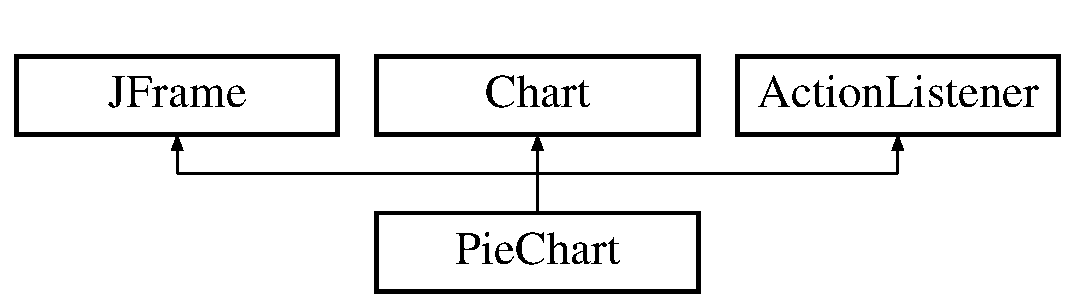
\includegraphics[height=2.000000cm]{class_pie_chart}
\end{center}
\end{figure}
\subsection*{Public Member Functions}
\begin{DoxyCompactItemize}
\item 
\hyperlink{class_pie_chart_a14e2a6c33b864d41debeb28df658286d}{Pie\-Chart} (String\mbox{[}$\,$\mbox{]}\mbox{[}$\,$\mbox{]} data, \hyperlink{class_dataset}{Dataset} dataset, \hyperlink{class_data_attribute}{Data\-Attribute} setting)
\item 
\hyperlink{class_pie_chart_aa7d3ab5c52b817c6731e1430831eaf39}{Pie\-Chart} (String\mbox{[}$\,$\mbox{]}\mbox{[}$\,$\mbox{]} data, \hyperlink{class_dataset}{Dataset} dataset, \hyperlink{class_data_attribute}{Data\-Attribute} setting, String\mbox{[}$\,$\mbox{]}\mbox{[}$\,$\mbox{]} second\-Data, \hyperlink{class_dataset}{Dataset} second\-Dataset, \hyperlink{class_data_attribute}{Data\-Attribute} second\-Setting)
\item 
\hyperlink{class_pie_chart_a122d771ebfd985bcb2b93e7f44719d0f}{Pie\-Chart} (\hyperlink{class_data_attribute}{Data\-Attribute} setting)
\item 
\hyperlink{class_pie_chart_aa2069046c7fa130fee473e17f57f570b}{Pie\-Chart} (\hyperlink{class_data_attribute}{Data\-Attribute} setting, \hyperlink{class_data_attribute}{Data\-Attribute} second\-Setting)
\item 
String\mbox{[}$\,$\mbox{]}\mbox{[}$\,$\mbox{]} \hyperlink{class_pie_chart_a7916d8aa39dbd1c48a1dac3cd3245f23}{Get\-Data} ()
\item 
int \hyperlink{class_pie_chart_a30b3ea3e7a0e5c53f50f3db916353346}{Get\-Index\-Count} ()
\item 
int \hyperlink{class_pie_chart_a3f104bd6d571abec5b8af8b43fdd96d7}{Get\-No\-Cols} ()
\item 
int \hyperlink{class_pie_chart_afbfbd6da7482a63d068c644e9e8cb149}{Get\-No\-Rows} ()
\item 
String \hyperlink{class_pie_chart_a2c5f499766ccbe0f5a537910a372fd6e}{Set\-Label\-X} (String x\-Label)
\item 
boolean \hyperlink{class_pie_chart_aeea92be8ab84aa78e56ec5c4f90e308b}{Set\-Data} (String\mbox{[}$\,$\mbox{]}\mbox{[}$\,$\mbox{]} data)
\item 
boolean \hyperlink{class_pie_chart_ad7812a5d88a05da851be00ac4728126c}{Set\-Index\-Count} (int index)
\item 
boolean \hyperlink{class_pie_chart_a0807bdf531833bcfa2ef97228ddfa770}{Set\-No\-Cols} (int cols)
\item 
boolean \hyperlink{class_pie_chart_ae80bc11611782f66bd3ad990baee963c}{Set\-No\-Rows} (int rows)
\item 
String \hyperlink{class_pie_chart_a2f762d12501691aa33335f33f1931f24}{Set\-Title} (String m\-\_\-chart\-Title)
\item 
void \hyperlink{class_pie_chart_ae30b814928c5a4bedb0cb86b48e18554}{action\-Performed} (Action\-Event e)
\item 
J\-Free\-Chart \hyperlink{class_pie_chart_abd00d9a07161c3fbf10bd6f19ec2750d}{Create\-Chart} (Pie\-Dataset dataset)
\item 
J\-Free\-Chart \hyperlink{class_pie_chart_afc121f4cb3d27f073711e844b7c26377}{Create\-Second\-Chart} (Pie\-Dataset dataset)
\item 
Boolean \hyperlink{class_pie_chart_aa9e53463d5ff3f5326fb92b25c89f349}{Show\-Chart} (Pie\-Dataset data)
\item 
Boolean \hyperlink{class_pie_chart_a38434bdbcc72eb384482dd372908e0ae}{Show\-Chart} (Pie\-Dataset data, Pie\-Dataset second\-Data)
\end{DoxyCompactItemize}
\subsection*{Static Public Member Functions}
\begin{DoxyCompactItemize}
\item 
static void \hyperlink{class_pie_chart_ab7e3bd074d520005660abe66a4ff00ff}{main} (String\mbox{[}$\,$\mbox{]} args)
\end{DoxyCompactItemize}


\subsection{Detailed Description}
A simple class that displays data in a single Pie \hyperlink{interface_chart}{Chart}, or two Pie \hyperlink{interface_chart}{Chart} visualisations. 

\begin{DoxyDate}{Date}
30/04/2013 
\end{DoxyDate}


\subsection{Constructor \& Destructor Documentation}
\hypertarget{class_pie_chart_a14e2a6c33b864d41debeb28df658286d}{\index{Pie\-Chart@{Pie\-Chart}!Pie\-Chart@{Pie\-Chart}}
\index{Pie\-Chart@{Pie\-Chart}!PieChart@{Pie\-Chart}}
\subsubsection[{Pie\-Chart}]{\setlength{\rightskip}{0pt plus 5cm}Pie\-Chart.\-Pie\-Chart (
\begin{DoxyParamCaption}
\item[{String}]{data\mbox{[}$\,$\mbox{]}\mbox{[}$\,$\mbox{]}, }
\item[{{\bf Dataset}}]{dataset, }
\item[{{\bf Data\-Attribute}}]{setting}
\end{DoxyParamCaption}
)}}\label{class_pie_chart_a14e2a6c33b864d41debeb28df658286d}

\begin{DoxyParams}{Parameters}
{\em String\mbox{[}$\,$\mbox{]}\mbox{[}$\,$\mbox{]}} & data -\/ data used to create the visualisation. \\
\hline
{\em \hyperlink{class_dataset}{Dataset}} & dataset -\/ the dataset used (rows and columns) \\
\hline
{\em \hyperlink{class_data_attribute}{Data\-Attribute}} & setting -\/ Data attributes \\
\hline
\end{DoxyParams}

\begin{DoxyCode}
34                                             \{
35         
36         m\_Data = data;
37         m\_ChartTitle = setting.\hyperlink{class_data_attribute_ade9747a192ba22fe1020e874bff6a48c}{GetTitle}();
38         m\_Setting = setting;
39         m\_XLabel = setting.\hyperlink{class_data_attribute_aecb451704a87d77dd80dbad8a19099d1}{GetAxisLabelX}();
40         m\_YLabel = setting.\hyperlink{class_data_attribute_af5f68794cd0195d42135d5e48120ccc0}{GetAxisLabelY}();
41         m\_Col = dataset.\hyperlink{class_dataset_ab922bef50c8aa1531de8704731779246}{GetNoOfCols}();
42         m\_Row = dataset.\hyperlink{class_dataset_a91257a605317576e87e1c32e54739e51}{GetNoOfRows}();
43         m\_C1 = setting.\hyperlink{class_data_attribute_a0f4a54973bc44b0526f78bda945dc81b}{GetSelectedXIndex}();
44         m\_C2 = setting.\hyperlink{class_data_attribute_a82e7519853d9f470ea183dd0c39a03d6}{GetSelectedYIndex}();
45         
46         m\_XMin = setting.\hyperlink{class_data_attribute_afa9da883abc4abad5f64c045de114c50}{GetXAxisMin}();
47         m\_XMax = setting.\hyperlink{class_data_attribute_a81243eb8f7008e05e74b0f3571d2f08d}{GetYAxisMax}();
48         m\_XScale = setting.\hyperlink{class_data_attribute_a5a1de25600487aa958a19ce01151fea4}{GetXAxisScale}();
49         m\_YScale = setting.\hyperlink{class_data_attribute_a95259727ce91efc0e0eaa28487d944c5}{GetYAxisScale}();
50         
51         CreateDataset( m\_Data );
52         \hyperlink{class_pie_chart_aa9e53463d5ff3f5326fb92b25c89f349}{ShowChart}( m\_dataset );
53     \}
\end{DoxyCode}
\hypertarget{class_pie_chart_aa7d3ab5c52b817c6731e1430831eaf39}{\index{Pie\-Chart@{Pie\-Chart}!Pie\-Chart@{Pie\-Chart}}
\index{Pie\-Chart@{Pie\-Chart}!PieChart@{Pie\-Chart}}
\subsubsection[{Pie\-Chart}]{\setlength{\rightskip}{0pt plus 5cm}Pie\-Chart.\-Pie\-Chart (
\begin{DoxyParamCaption}
\item[{String}]{data\mbox{[}$\,$\mbox{]}\mbox{[}$\,$\mbox{]}, }
\item[{{\bf Dataset}}]{dataset, }
\item[{{\bf Data\-Attribute}}]{setting, }
\item[{String}]{second\-Data\mbox{[}$\,$\mbox{]}\mbox{[}$\,$\mbox{]}, }
\item[{{\bf Dataset}}]{second\-Dataset, }
\item[{{\bf Data\-Attribute}}]{second\-Setting}
\end{DoxyParamCaption}
)}}\label{class_pie_chart_aa7d3ab5c52b817c6731e1430831eaf39}
creates a constructor taking in the following parameters\-:


\begin{DoxyParams}{Parameters}
{\em String\mbox{[}$\,$\mbox{]}\mbox{[}$\,$\mbox{]}} & data -\/ data used to create the visualisation. \\
\hline
{\em \hyperlink{class_dataset}{Dataset}} & dataset -\/ the dataset used (rows and columns) \\
\hline
{\em \hyperlink{class_data_attribute}{Data\-Attribute}} & setting -\/ Data attributes \\
\hline
{\em String\mbox{[}$\,$\mbox{]}\mbox{[}$\,$\mbox{]}} & second\-Data -\/ second data used to create the visualisation. \\
\hline
{\em \hyperlink{class_dataset}{Dataset}} & second\-Dataset -\/ the second dataset used (rows and columns) \\
\hline
{\em \hyperlink{class_data_attribute}{Data\-Attribute}} & second\-Setting -\/ Second Data attributes \\
\hline
\end{DoxyParams}

\begin{DoxyCode}
66                                          \{
67 
68         m\_Data = data;
69         m\_ChartTitle = setting.\hyperlink{class_data_attribute_ade9747a192ba22fe1020e874bff6a48c}{GetTitle}();
70         m\_Setting = setting;
71         m\_XLabel = setting.\hyperlink{class_data_attribute_aecb451704a87d77dd80dbad8a19099d1}{GetAxisLabelX}();
72         m\_YLabel = setting.\hyperlink{class_data_attribute_af5f68794cd0195d42135d5e48120ccc0}{GetAxisLabelY}();
73         m\_Col = dataset.\hyperlink{class_dataset_ab922bef50c8aa1531de8704731779246}{GetNoOfCols}();
74         m\_Row = dataset.\hyperlink{class_dataset_a91257a605317576e87e1c32e54739e51}{GetNoOfRows}();
75         m\_C1 = setting.\hyperlink{class_data_attribute_a0f4a54973bc44b0526f78bda945dc81b}{GetSelectedXIndex}();
76         m\_C2 = setting.\hyperlink{class_data_attribute_a82e7519853d9f470ea183dd0c39a03d6}{GetSelectedYIndex}();
77         
78         m\_SecondData = data;
79         m\_SecondChartTitle = setting.\hyperlink{class_data_attribute_a4079522c93025fce7569eaed585f4aeb}{GetSecondTitle}();
80         m\_SecondSetting = secondSetting;
81         m\_SecondXLabel = setting.\hyperlink{class_data_attribute_a8ace4cb1fee9e2abeabe3efc9a190c8f}{GetSecondAxisLabelX}();
82         m\_SecondYLabel = setting.\hyperlink{class_data_attribute_a6efb7e067317898feefbbf6bd472b998}{GetSecondAxisLabelY}();
83         m\_SecondCol = dataset.\hyperlink{class_dataset_ab922bef50c8aa1531de8704731779246}{GetNoOfCols}();
84         m\_SecondRow = dataset.\hyperlink{class_dataset_a91257a605317576e87e1c32e54739e51}{GetNoOfRows}();
85         m\_SecondC1 = setting.\hyperlink{class_data_attribute_a7f501790eee650ddf9ac17c4f63a3995}{GetSecondSelectedXIndex}();
86         m\_SecondC2 = setting.\hyperlink{class_data_attribute_a6f61ad05915f4aa31ad3dba00596da64}{GetSecondSelectedYIndex}();
87         
88         m\_XMin = setting.\hyperlink{class_data_attribute_afa9da883abc4abad5f64c045de114c50}{GetXAxisMin}();
89         m\_XMax = setting.\hyperlink{class_data_attribute_a81243eb8f7008e05e74b0f3571d2f08d}{GetYAxisMax}();
90         m\_XScale = setting.\hyperlink{class_data_attribute_a5a1de25600487aa958a19ce01151fea4}{GetXAxisScale}();
91         m\_YScale = setting.\hyperlink{class_data_attribute_a95259727ce91efc0e0eaa28487d944c5}{GetYAxisScale}();
92         
93         m\_SecondXMin = setting.\hyperlink{class_data_attribute_afa9da883abc4abad5f64c045de114c50}{GetXAxisMin}();
94         m\_SecondXMax = setting.\hyperlink{class_data_attribute_a81243eb8f7008e05e74b0f3571d2f08d}{GetYAxisMax}();
95         m\_SecondXScale = setting.\hyperlink{class_data_attribute_a5a1de25600487aa958a19ce01151fea4}{GetXAxisScale}();
96         m\_SecondYScale = setting.\hyperlink{class_data_attribute_a95259727ce91efc0e0eaa28487d944c5}{GetYAxisScale}();
97         
98 
99         CreateDataset( m\_Data );
100         CreateSecondDataset(m\_SecondData);
101         \hyperlink{class_pie_chart_aa9e53463d5ff3f5326fb92b25c89f349}{ShowChart}( m\_dataset, m\_secondDataset );       
102     \}
\end{DoxyCode}
\hypertarget{class_pie_chart_a122d771ebfd985bcb2b93e7f44719d0f}{\index{Pie\-Chart@{Pie\-Chart}!Pie\-Chart@{Pie\-Chart}}
\index{Pie\-Chart@{Pie\-Chart}!PieChart@{Pie\-Chart}}
\subsubsection[{Pie\-Chart}]{\setlength{\rightskip}{0pt plus 5cm}Pie\-Chart.\-Pie\-Chart (
\begin{DoxyParamCaption}
\item[{{\bf Data\-Attribute}}]{setting}
\end{DoxyParamCaption}
)}}\label{class_pie_chart_a122d771ebfd985bcb2b93e7f44719d0f}
constructor for J\-Unit Tests 
\begin{DoxyParams}{Parameters}
{\em setting} & \\
\hline
\end{DoxyParams}

\begin{DoxyCode}
107                                            \{
108         
109         m\_Setting = setting;
110         m\_ChartTitle = setting.\hyperlink{class_data_attribute_ade9747a192ba22fe1020e874bff6a48c}{GetTitle}();
111         m\_XLabel = setting.\hyperlink{class_data_attribute_aecb451704a87d77dd80dbad8a19099d1}{GetAxisLabelX}();
112         m\_YLabel = setting.\hyperlink{class_data_attribute_af5f68794cd0195d42135d5e48120ccc0}{GetAxisLabelY}();
113         m\_C1 = setting.\hyperlink{class_data_attribute_a0f4a54973bc44b0526f78bda945dc81b}{GetSelectedXIndex}();
114         m\_C2 = setting.\hyperlink{class_data_attribute_a82e7519853d9f470ea183dd0c39a03d6}{GetSelectedYIndex}();
115         
116         m\_XMin = setting.\hyperlink{class_data_attribute_afa9da883abc4abad5f64c045de114c50}{GetXAxisMin}();
117         m\_XMax = setting.\hyperlink{class_data_attribute_a81243eb8f7008e05e74b0f3571d2f08d}{GetYAxisMax}();
118         m\_XScale = setting.\hyperlink{class_data_attribute_a5a1de25600487aa958a19ce01151fea4}{GetXAxisScale}();
119         m\_YScale = setting.\hyperlink{class_data_attribute_a95259727ce91efc0e0eaa28487d944c5}{GetYAxisScale}();
120     \}
\end{DoxyCode}
\hypertarget{class_pie_chart_aa2069046c7fa130fee473e17f57f570b}{\index{Pie\-Chart@{Pie\-Chart}!Pie\-Chart@{Pie\-Chart}}
\index{Pie\-Chart@{Pie\-Chart}!PieChart@{Pie\-Chart}}
\subsubsection[{Pie\-Chart}]{\setlength{\rightskip}{0pt plus 5cm}Pie\-Chart.\-Pie\-Chart (
\begin{DoxyParamCaption}
\item[{{\bf Data\-Attribute}}]{setting, }
\item[{{\bf Data\-Attribute}}]{second\-Setting}
\end{DoxyParamCaption}
)}}\label{class_pie_chart_aa2069046c7fa130fee473e17f57f570b}
second empty constructor for J\-Unit Tests 
\begin{DoxyParams}{Parameters}
{\em setting} & \\
\hline
{\em second\-Setting} & \\
\hline
\end{DoxyParams}

\begin{DoxyCode}
127                                                                         \{
128         
129         m\_Setting = setting;
130         m\_ChartTitle = setting.\hyperlink{class_data_attribute_ade9747a192ba22fe1020e874bff6a48c}{GetTitle}();
131         m\_XLabel = setting.\hyperlink{class_data_attribute_aecb451704a87d77dd80dbad8a19099d1}{GetAxisLabelX}();
132         m\_YLabel = setting.\hyperlink{class_data_attribute_af5f68794cd0195d42135d5e48120ccc0}{GetAxisLabelY}();
133         m\_C1 = setting.\hyperlink{class_data_attribute_a0f4a54973bc44b0526f78bda945dc81b}{GetSelectedXIndex}();
134         m\_C2 = setting.\hyperlink{class_data_attribute_a82e7519853d9f470ea183dd0c39a03d6}{GetSelectedYIndex}();
135         
136         m\_XMin = setting.\hyperlink{class_data_attribute_afa9da883abc4abad5f64c045de114c50}{GetXAxisMin}();
137         m\_XMax = setting.\hyperlink{class_data_attribute_a81243eb8f7008e05e74b0f3571d2f08d}{GetYAxisMax}();
138         m\_XScale = setting.\hyperlink{class_data_attribute_a5a1de25600487aa958a19ce01151fea4}{GetXAxisScale}();
139         m\_YScale = setting.\hyperlink{class_data_attribute_a95259727ce91efc0e0eaa28487d944c5}{GetYAxisScale}();
140         
141         m\_SecondSetting = secondSetting;
142         m\_SecondChartTitle = secondSetting.\hyperlink{class_data_attribute_a4079522c93025fce7569eaed585f4aeb}{GetSecondTitle}();
143         m\_SecondXLabel = secondSetting.\hyperlink{class_data_attribute_a8ace4cb1fee9e2abeabe3efc9a190c8f}{GetSecondAxisLabelX}();
144         m\_SecondYLabel = secondSetting.\hyperlink{class_data_attribute_a6efb7e067317898feefbbf6bd472b998}{GetSecondAxisLabelY}();
145         m\_SecondC1 = secondSetting.\hyperlink{class_data_attribute_a7f501790eee650ddf9ac17c4f63a3995}{GetSecondSelectedXIndex}();
146         m\_SecondC2 = secondSetting.\hyperlink{class_data_attribute_a6f61ad05915f4aa31ad3dba00596da64}{GetSecondSelectedYIndex}();
147         
148         m\_SecondXMin = secondSetting.\hyperlink{class_data_attribute_afa9da883abc4abad5f64c045de114c50}{GetXAxisMin}();
149         m\_SecondXMax = secondSetting.\hyperlink{class_data_attribute_a81243eb8f7008e05e74b0f3571d2f08d}{GetYAxisMax}();
150         m\_SecondXScale = secondSetting.\hyperlink{class_data_attribute_a5a1de25600487aa958a19ce01151fea4}{GetXAxisScale}();
151         m\_SecondYScale = secondSetting.\hyperlink{class_data_attribute_a95259727ce91efc0e0eaa28487d944c5}{GetYAxisScale}();
152     \}
\end{DoxyCode}


\subsection{Member Function Documentation}
\hypertarget{class_pie_chart_ae30b814928c5a4bedb0cb86b48e18554}{\index{Pie\-Chart@{Pie\-Chart}!action\-Performed@{action\-Performed}}
\index{action\-Performed@{action\-Performed}!PieChart@{Pie\-Chart}}
\subsubsection[{action\-Performed}]{\setlength{\rightskip}{0pt plus 5cm}void Pie\-Chart.\-action\-Performed (
\begin{DoxyParamCaption}
\item[{Action\-Event}]{e}
\end{DoxyParamCaption}
)}}\label{class_pie_chart_ae30b814928c5a4bedb0cb86b48e18554}

\begin{DoxyParams}{Parameters}
{\em e} & -\/ action button to allow choosers to select a colour \\
\hline
\end{DoxyParams}

\begin{DoxyCode}
279                                                  \{
280         \textcolor{keywordflow}{if}( e.getSource() == colChangeButton ) \{
281             \hyperlink{class_colour_map}{ColourMap} cM = \textcolor{keyword}{new} \hyperlink{class_colour_map}{ColourMap}();
282             cM.\hyperlink{class_colour_map_a9f696ea699b7fc471bb2dde6f1d1ce09}{SetupData}( m\_IndexCount,plotChart );
283             cM.setVisible( \textcolor{keyword}{false} );
284         \}
285     \}
\end{DoxyCode}
\hypertarget{class_pie_chart_abd00d9a07161c3fbf10bd6f19ec2750d}{\index{Pie\-Chart@{Pie\-Chart}!Create\-Chart@{Create\-Chart}}
\index{Create\-Chart@{Create\-Chart}!PieChart@{Pie\-Chart}}
\subsubsection[{Create\-Chart}]{\setlength{\rightskip}{0pt plus 5cm}J\-Free\-Chart Pie\-Chart.\-Create\-Chart (
\begin{DoxyParamCaption}
\item[{Pie\-Dataset}]{dataset}
\end{DoxyParamCaption}
)}}\label{class_pie_chart_abd00d9a07161c3fbf10bd6f19ec2750d}
create the 3\-D pie chart and set the appearance 
\begin{DoxyParams}{Parameters}
{\em dataset} & -\/ pass the pie dataset through \\
\hline
{\em chart\-Title} & -\/ pass through the chart title \\
\hline
\end{DoxyParams}
\begin{DoxyReturn}{Returns}
-\/ a 3\-D piechart 
\end{DoxyReturn}

\begin{DoxyCode}
293                                                         \{
294         
295         JFreeChart chart = ChartFactory.createPieChart3D( 
296                 m\_ChartTitle,
297             m\_dataset, \textcolor{keyword}{true},                          
298             \textcolor{keyword}{true}, \textcolor{keyword}{false} );
299         
300         \textcolor{comment}{//xyPlot = chart.getXYPlot();}
301         plotChart  = ( PiePlot3D ) chart.getPlot();      
302         plotChart.setStartAngle( START\_ANGLE );
303         plotChart.setDirection( Rotation.CLOCKWISE ); 
304         plotChart.setForegroundAlpha(TRANSPARENCY); 
305         \textcolor{keywordflow}{return} chart;       
306     \}
\end{DoxyCode}
\hypertarget{class_pie_chart_afc121f4cb3d27f073711e844b7c26377}{\index{Pie\-Chart@{Pie\-Chart}!Create\-Second\-Chart@{Create\-Second\-Chart}}
\index{Create\-Second\-Chart@{Create\-Second\-Chart}!PieChart@{Pie\-Chart}}
\subsubsection[{Create\-Second\-Chart}]{\setlength{\rightskip}{0pt plus 5cm}J\-Free\-Chart Pie\-Chart.\-Create\-Second\-Chart (
\begin{DoxyParamCaption}
\item[{Pie\-Dataset}]{dataset}
\end{DoxyParamCaption}
)}}\label{class_pie_chart_afc121f4cb3d27f073711e844b7c26377}
creates the second 3\-D pie chart and set the appearance 
\begin{DoxyParams}{Parameters}
{\em dataset} & -\/ pass the pie dataset through \\
\hline
{\em secon\-Chart\-Title} & -\/ pass through the second chart title \\
\hline
\end{DoxyParams}
\begin{DoxyReturn}{Returns}
-\/ a 3\-D piechart 
\end{DoxyReturn}

\begin{DoxyCode}
313                                                               \{
314         JFreeChart chart = ChartFactory.createPieChart3D( 
315                 m\_SecondChartTitle,
316             m\_secondDataset, \textcolor{keyword}{true},                          
317             \textcolor{keyword}{true}, \textcolor{keyword}{false} );
318         
319         \textcolor{comment}{//xyPlot = chart.getXYPlot();}
320         plotChart  = ( PiePlot3D ) chart.getPlot();      
321         plotChart.setStartAngle( START\_ANGLE );
322         plotChart.setDirection( Rotation.CLOCKWISE ); 
323         plotChart.setForegroundAlpha(TRANSPARENCY); 
324         \textcolor{keywordflow}{return} chart;       
325     \}
\end{DoxyCode}
\hypertarget{class_pie_chart_a7916d8aa39dbd1c48a1dac3cd3245f23}{\index{Pie\-Chart@{Pie\-Chart}!Get\-Data@{Get\-Data}}
\index{Get\-Data@{Get\-Data}!PieChart@{Pie\-Chart}}
\subsubsection[{Get\-Data}]{\setlength{\rightskip}{0pt plus 5cm}String \mbox{[}$\,$\mbox{]}\mbox{[}$\,$\mbox{]} Pie\-Chart.\-Get\-Data (
\begin{DoxyParamCaption}
{}
\end{DoxyParamCaption}
)}}\label{class_pie_chart_a7916d8aa39dbd1c48a1dac3cd3245f23}
\begin{DoxyReturn}{Returns}
-\/ return a variable which stores the data. 
\end{DoxyReturn}

\begin{DoxyCode}
157                                 \{
158         \textcolor{keywordflow}{return} m\_Data;
159     \}
\end{DoxyCode}
\hypertarget{class_pie_chart_a30b3ea3e7a0e5c53f50f3db916353346}{\index{Pie\-Chart@{Pie\-Chart}!Get\-Index\-Count@{Get\-Index\-Count}}
\index{Get\-Index\-Count@{Get\-Index\-Count}!PieChart@{Pie\-Chart}}
\subsubsection[{Get\-Index\-Count}]{\setlength{\rightskip}{0pt plus 5cm}int Pie\-Chart.\-Get\-Index\-Count (
\begin{DoxyParamCaption}
{}
\end{DoxyParamCaption}
)}}\label{class_pie_chart_a30b3ea3e7a0e5c53f50f3db916353346}
\begin{DoxyReturn}{Returns}
-\/ return a variable with the current index of each pie slice. 
\end{DoxyReturn}

\begin{DoxyCode}
164                                \{
165         \textcolor{keywordflow}{return} m\_IndexCount;
166     \}
\end{DoxyCode}
\hypertarget{class_pie_chart_a3f104bd6d571abec5b8af8b43fdd96d7}{\index{Pie\-Chart@{Pie\-Chart}!Get\-No\-Cols@{Get\-No\-Cols}}
\index{Get\-No\-Cols@{Get\-No\-Cols}!PieChart@{Pie\-Chart}}
\subsubsection[{Get\-No\-Cols}]{\setlength{\rightskip}{0pt plus 5cm}int Pie\-Chart.\-Get\-No\-Cols (
\begin{DoxyParamCaption}
{}
\end{DoxyParamCaption}
)}}\label{class_pie_chart_a3f104bd6d571abec5b8af8b43fdd96d7}
\begin{DoxyReturn}{Returns}
-\/ a variable which returns the current number of columns 
\end{DoxyReturn}

\begin{DoxyCode}
170                            \{
171         \textcolor{keywordflow}{return} m\_Col;
172     \}
\end{DoxyCode}
\hypertarget{class_pie_chart_afbfbd6da7482a63d068c644e9e8cb149}{\index{Pie\-Chart@{Pie\-Chart}!Get\-No\-Rows@{Get\-No\-Rows}}
\index{Get\-No\-Rows@{Get\-No\-Rows}!PieChart@{Pie\-Chart}}
\subsubsection[{Get\-No\-Rows}]{\setlength{\rightskip}{0pt plus 5cm}int Pie\-Chart.\-Get\-No\-Rows (
\begin{DoxyParamCaption}
{}
\end{DoxyParamCaption}
)}}\label{class_pie_chart_afbfbd6da7482a63d068c644e9e8cb149}
\begin{DoxyReturn}{Returns}
-\/ a variable which returns the current number of rows 
\end{DoxyReturn}

\begin{DoxyCode}
176                            \{
177         \textcolor{keywordflow}{return} m\_Row;
178     \}
\end{DoxyCode}
\hypertarget{class_pie_chart_ab7e3bd074d520005660abe66a4ff00ff}{\index{Pie\-Chart@{Pie\-Chart}!main@{main}}
\index{main@{main}!PieChart@{Pie\-Chart}}
\subsubsection[{main}]{\setlength{\rightskip}{0pt plus 5cm}static void Pie\-Chart.\-main (
\begin{DoxyParamCaption}
\item[{String\mbox{[}$\,$\mbox{]}}]{args}
\end{DoxyParamCaption}
)\hspace{0.3cm}{\ttfamily [static]}}}\label{class_pie_chart_ab7e3bd074d520005660abe66a4ff00ff}
Main method which implement 3 unit tests for each 'set' method 
\begin{DoxyParams}{Parameters}
{\em args} & -\/ no user input needed \\
\hline
\end{DoxyParams}

\begin{DoxyCode}
452                                             \{
453         \hyperlink{class_data_attribute}{DataAttribute} test = \hyperlink{class_data_attribute}{DataAttribute}.
      \hyperlink{class_data_attribute_a9c7a1923698c1530fa38c959596199bc}{GetTestDataAttribute}();
454         \hyperlink{class_pie_chart}{PieChart} pieChartTest = \textcolor{keyword}{new} \hyperlink{class_pie_chart_a14e2a6c33b864d41debeb28df658286d}{PieChart}(test);
455         
456         \textcolor{keyword}{final} PieDataset datasetTest = createTestDataset();
457         pieChartTest.\hyperlink{class_pie_chart_aa9e53463d5ff3f5326fb92b25c89f349}{ShowChart}(datasetTest);
458         
459         \hyperlink{class_data_attribute}{DataAttribute} secondTest = \hyperlink{class_data_attribute}{DataAttribute}.
      \hyperlink{class_data_attribute_a9c7a1923698c1530fa38c959596199bc}{GetTestDataAttribute}();
460         \hyperlink{class_pie_chart}{PieChart} secondPieChartTest = \textcolor{keyword}{new} \hyperlink{class_pie_chart_a14e2a6c33b864d41debeb28df658286d}{PieChart}(secondTest);
461         
462         \textcolor{keyword}{final} PieDataset secondDatasetTest = createTestDataset();
463         secondPieChartTest.\hyperlink{class_pie_chart_aa9e53463d5ff3f5326fb92b25c89f349}{ShowChart}(datasetTest, secondDatasetTest);      
464     \}
\end{DoxyCode}
\hypertarget{class_pie_chart_aeea92be8ab84aa78e56ec5c4f90e308b}{\index{Pie\-Chart@{Pie\-Chart}!Set\-Data@{Set\-Data}}
\index{Set\-Data@{Set\-Data}!PieChart@{Pie\-Chart}}
\subsubsection[{Set\-Data}]{\setlength{\rightskip}{0pt plus 5cm}boolean Pie\-Chart.\-Set\-Data (
\begin{DoxyParamCaption}
\item[{String}]{data\mbox{[}$\,$\mbox{]}\mbox{[}$\,$\mbox{]}}
\end{DoxyParamCaption}
)}}\label{class_pie_chart_aeea92be8ab84aa78e56ec5c4f90e308b}

\begin{DoxyParams}{Parameters}
{\em data} & -\/ variable to test if m\-\_\-\-Int\-Data has any errors \\
\hline
\end{DoxyParams}
\begin{DoxyReturn}{Returns}
-\/ returns boolean if test is true 
\end{DoxyReturn}

\begin{DoxyCode}
197                                               \{
198         \textcolor{keywordtype}{boolean} test = \textcolor{keyword}{true};
199         \textcolor{keywordflow}{if} ( data == null && test == \textcolor{keyword}{true} ) \{
200             System.err.println( \textcolor{stringliteral}{"PieChart::setData() ***Warning, data set to: "} 
201                     + data );
202         \}
203         \textcolor{keywordflow}{else} \textcolor{keywordflow}{if} ( test == \textcolor{keyword}{true} ) \{
204             System.out.println( \textcolor{stringliteral}{"PieChart::setData() file location set to: "}
205                     + data );
206         \}
207             m\_Data = data;
208             \textcolor{keywordflow}{return} \textcolor{keyword}{true};
209     \}
\end{DoxyCode}
\hypertarget{class_pie_chart_ad7812a5d88a05da851be00ac4728126c}{\index{Pie\-Chart@{Pie\-Chart}!Set\-Index\-Count@{Set\-Index\-Count}}
\index{Set\-Index\-Count@{Set\-Index\-Count}!PieChart@{Pie\-Chart}}
\subsubsection[{Set\-Index\-Count}]{\setlength{\rightskip}{0pt plus 5cm}boolean Pie\-Chart.\-Set\-Index\-Count (
\begin{DoxyParamCaption}
\item[{int}]{index}
\end{DoxyParamCaption}
)}}\label{class_pie_chart_ad7812a5d88a05da851be00ac4728126c}

\begin{DoxyParams}{Parameters}
{\em index} & -\/ variable to test if m\-\_\-\-Index\-Count has any errors \\
\hline
\end{DoxyParams}
\begin{DoxyReturn}{Returns}
-\/ returns boolean if test is true 
\end{DoxyReturn}

\begin{DoxyCode}
214                                               \{
215         \textcolor{keywordtype}{boolean} test = \textcolor{keyword}{true};
216         \textcolor{keywordflow}{if} ( index < 0 && test == \textcolor{keyword}{true} ) \{
217             System.err.println( \textcolor{stringliteral}{"PieChart::setIndexCount() ***Warning, index "}
218                         + \textcolor{stringliteral}{"set to: "} + index );
219         \}
220         \textcolor{keywordflow}{else} \textcolor{keywordflow}{if} ( test == \textcolor{keyword}{true} ) \{
221             System.out.println( \textcolor{stringliteral}{"PieChart::setIndexCount() index set to: "} 
222                     + index );
223         \}
224         m\_IndexCount = index;
225         \textcolor{keywordflow}{return} \textcolor{keyword}{true};
226     \}
\end{DoxyCode}
\hypertarget{class_pie_chart_a2c5f499766ccbe0f5a537910a372fd6e}{\index{Pie\-Chart@{Pie\-Chart}!Set\-Label\-X@{Set\-Label\-X}}
\index{Set\-Label\-X@{Set\-Label\-X}!PieChart@{Pie\-Chart}}
\subsubsection[{Set\-Label\-X}]{\setlength{\rightskip}{0pt plus 5cm}String Pie\-Chart.\-Set\-Label\-X (
\begin{DoxyParamCaption}
\item[{String}]{x\-Label}
\end{DoxyParamCaption}
)}}\label{class_pie_chart_a2c5f499766ccbe0f5a537910a372fd6e}

\begin{DoxyParams}{Parameters}
{\em x\-Label} & -\/ the x\-Label to be passed from the users to the chart \\
\hline
\end{DoxyParams}

\begin{DoxyCode}
183                                              \{
184         \textcolor{keywordtype}{boolean} test = \textcolor{keyword}{true};
185         
186         \textcolor{keywordflow}{if} ( ( ( xLabel.isEmpty() )||( xLabel.length() > MAX\_LABEL\_LENGTH ) ) 
187                && ( test == true ) ) \{
188             System.err.println( \textcolor{stringliteral}{"ScatterPlotGraph::SetLabelX "} + xLabel );
189     \}
190         
191         \textcolor{keywordflow}{return} xLabel;
192     \}
\end{DoxyCode}
\hypertarget{class_pie_chart_a0807bdf531833bcfa2ef97228ddfa770}{\index{Pie\-Chart@{Pie\-Chart}!Set\-No\-Cols@{Set\-No\-Cols}}
\index{Set\-No\-Cols@{Set\-No\-Cols}!PieChart@{Pie\-Chart}}
\subsubsection[{Set\-No\-Cols}]{\setlength{\rightskip}{0pt plus 5cm}boolean Pie\-Chart.\-Set\-No\-Cols (
\begin{DoxyParamCaption}
\item[{int}]{cols}
\end{DoxyParamCaption}
)}}\label{class_pie_chart_a0807bdf531833bcfa2ef97228ddfa770}

\begin{DoxyParams}{Parameters}
{\em cols} & -\/ variable to test if m\-\_\-\-No\-Of\-Cols has any errors \\
\hline
\end{DoxyParams}
\begin{DoxyReturn}{Returns}
-\/ returns boolean if test is true 
\end{DoxyReturn}

\begin{DoxyCode}
231                                          \{
232         \textcolor{keywordtype}{boolean} test = \textcolor{keyword}{true};
233         \textcolor{keywordflow}{if} ( cols < 0 && test == \textcolor{keyword}{true} ) \{
234             System.err.println( \textcolor{stringliteral}{"PieChart::setNoCols() ***Warning, cols "}
235                         + \textcolor{stringliteral}{"set to: "} + cols );
236         \}
237         \textcolor{keywordflow}{else} \textcolor{keywordflow}{if} ( test == \textcolor{keyword}{true} ) \{
238             System.out.println( \textcolor{stringliteral}{"PieChart::setNoCols() cols set to: "} 
239                     + cols );
240         \}
241         m\_Col = cols;
242         \textcolor{keywordflow}{return} \textcolor{keyword}{true};
243     \}
\end{DoxyCode}
\hypertarget{class_pie_chart_ae80bc11611782f66bd3ad990baee963c}{\index{Pie\-Chart@{Pie\-Chart}!Set\-No\-Rows@{Set\-No\-Rows}}
\index{Set\-No\-Rows@{Set\-No\-Rows}!PieChart@{Pie\-Chart}}
\subsubsection[{Set\-No\-Rows}]{\setlength{\rightskip}{0pt plus 5cm}boolean Pie\-Chart.\-Set\-No\-Rows (
\begin{DoxyParamCaption}
\item[{int}]{rows}
\end{DoxyParamCaption}
)}}\label{class_pie_chart_ae80bc11611782f66bd3ad990baee963c}

\begin{DoxyParams}{Parameters}
{\em rows} & -\/ variable to test if m\-\_\-\-No\-Of\-Rows has any errors \\
\hline
\end{DoxyParams}
\begin{DoxyReturn}{Returns}
-\/ returns boolean if test is true 
\end{DoxyReturn}

\begin{DoxyCode}
248                                          \{
249         \textcolor{keywordtype}{boolean} test = \textcolor{keyword}{true};
250         \textcolor{keywordflow}{if} ( rows < 0 && test == \textcolor{keyword}{true} ) \{
251             System.err.println( \textcolor{stringliteral}{"PieChart::setNoRows() ***Warning, rows "}
252                         + \textcolor{stringliteral}{"set to: "} + rows );
253         \}
254         \textcolor{keywordflow}{else} \textcolor{keywordflow}{if} ( test == \textcolor{keyword}{true} ) \{
255             System.out.println( \textcolor{stringliteral}{"PieChart::setNoRows() rows set to: "} 
256                     + rows );
257         \}
258         m\_Row = rows;
259         \textcolor{keywordflow}{return} \textcolor{keyword}{true};
260     \}
\end{DoxyCode}
\hypertarget{class_pie_chart_a2f762d12501691aa33335f33f1931f24}{\index{Pie\-Chart@{Pie\-Chart}!Set\-Title@{Set\-Title}}
\index{Set\-Title@{Set\-Title}!PieChart@{Pie\-Chart}}
\subsubsection[{Set\-Title}]{\setlength{\rightskip}{0pt plus 5cm}String Pie\-Chart.\-Set\-Title (
\begin{DoxyParamCaption}
\item[{String}]{m\-\_\-chart\-Title}
\end{DoxyParamCaption}
)}}\label{class_pie_chart_a2f762d12501691aa33335f33f1931f24}

\begin{DoxyParams}{Parameters}
{\em m\-\_\-chart\-Title} & -\/ the title to be passed from users for the chart \\
\hline
\end{DoxyParams}

\begin{DoxyCode}
265                                                   \{
266         \textcolor{keywordtype}{boolean} test = \textcolor{keyword}{true};
267         
268         \textcolor{keywordflow}{if} ( ( ( m\_chartTitle.isEmpty() )||( m\_chartTitle.length() > MAX\_CHART\_TITLE\_LENGTH ) )
269                && ( test == true ) ) \{
270             System.err.println( \textcolor{stringliteral}{"ScatterPlotGraph::SetTitle "} + m\_chartTitle );
271         \}
272         
273         \textcolor{keywordflow}{return} m\_chartTitle;
274     \}
\end{DoxyCode}
\hypertarget{class_pie_chart_aa9e53463d5ff3f5326fb92b25c89f349}{\index{Pie\-Chart@{Pie\-Chart}!Show\-Chart@{Show\-Chart}}
\index{Show\-Chart@{Show\-Chart}!PieChart@{Pie\-Chart}}
\subsubsection[{Show\-Chart}]{\setlength{\rightskip}{0pt plus 5cm}Boolean Pie\-Chart.\-Show\-Chart (
\begin{DoxyParamCaption}
\item[{Pie\-Dataset}]{data}
\end{DoxyParamCaption}
)}}\label{class_pie_chart_aa9e53463d5ff3f5326fb92b25c89f349}
visualises the Pie chart using J\-Free\-Chart and sets the default size and appearance of the window and graph


\begin{DoxyParams}{Parameters}
{\em datas} & -\/ passes the Pie data through \\
\hline
\end{DoxyParams}
\begin{DoxyReturn}{Returns}
true -\/ returns test results 
\end{DoxyReturn}

\begin{DoxyCode}
369                                               \{
370         JFreeChart chart = \hyperlink{class_pie_chart_abd00d9a07161c3fbf10bd6f19ec2750d}{CreateChart}(data);         
371         ChartPanel chartPanel = \textcolor{keyword}{new} ChartPanel( chart );           
372                 
373         \textcolor{comment}{/* instantiate colour options */}
374         JPanel colourButtonPanel = \textcolor{keyword}{new} JPanel( \textcolor{keyword}{new} BorderLayout() );
375         colChangeButton = \textcolor{keyword}{new} JButton( \textcolor{stringliteral}{"Change Colours"} );
376         colourButtonPanel.add( colChangeButton,BorderLayout.SOUTH );
377         colChangeButton.addActionListener( \hyperlink{class_pie_chart}{PieChart}.this );
378         
379         JFrame test = \textcolor{keyword}{new} JFrame();
380         test.setLayout(\textcolor{keyword}{new} BorderLayout());
381         test.setSize( FRAME\_WIDTH, FRAME\_HEIGHT );
382         test.setTitle(\textcolor{stringliteral}{"Pie Chart"});
383         test.setDefaultCloseOperation(JFrame.DISPOSE\_ON\_CLOSE);
384         test.add(chartPanel, BorderLayout.NORTH);
385         test.add(\textcolor{keyword}{new} \hyperlink{class_information_j_panel}{InformationJPanel}(m\_Setting), BorderLayout.CENTER);
386         test.add(colourButtonPanel, BorderLayout.SOUTH);
387         test.setVisible(\textcolor{keyword}{true});
388         
389         \textcolor{keywordflow}{return} \textcolor{keyword}{true};
390     \}
\end{DoxyCode}
\hypertarget{class_pie_chart_a38434bdbcc72eb384482dd372908e0ae}{\index{Pie\-Chart@{Pie\-Chart}!Show\-Chart@{Show\-Chart}}
\index{Show\-Chart@{Show\-Chart}!PieChart@{Pie\-Chart}}
\subsubsection[{Show\-Chart}]{\setlength{\rightskip}{0pt plus 5cm}Boolean Pie\-Chart.\-Show\-Chart (
\begin{DoxyParamCaption}
\item[{Pie\-Dataset}]{data, }
\item[{Pie\-Dataset}]{second\-Data}
\end{DoxyParamCaption}
)}}\label{class_pie_chart_a38434bdbcc72eb384482dd372908e0ae}
visualises the Pie chart using J\-Free\-Chart and sets the default size and appearance of the window and graph


\begin{DoxyParams}{Parameters}
{\em data} & -\/ passes the Pie data through \\
\hline
{\em second\-Data} & -\/ passes the second Pie data through \\
\hline
\end{DoxyParams}
\begin{DoxyReturn}{Returns}
true -\/ returns test results 
\end{DoxyReturn}

\begin{DoxyCode}
399                                                                      \{
400         JFreeChart chart = \hyperlink{class_pie_chart_abd00d9a07161c3fbf10bd6f19ec2750d}{CreateChart}(data);
401         JFreeChart secondChart = \hyperlink{class_pie_chart_afc121f4cb3d27f073711e844b7c26377}{CreateSecondChart}(data);
402         ChartPanel chartPanel = \textcolor{keyword}{new} ChartPanel( chart );           
403         ChartPanel secondChartPanel = \textcolor{keyword}{new} ChartPanel( secondChart );  
404         chartPanel.setPreferredSize( \textcolor{keyword}{new} java.awt.Dimension( CHART\_WIDTH, CHART\_HEIGHT ) );
405         secondChartPanel.setPreferredSize( \textcolor{keyword}{new} java.awt.Dimension( CHART\_WIDTH, CHART\_HEIGHT ) );
406                 
407         \textcolor{comment}{/* instantiate colour options */}
408         JPanel colourButtonPanel = \textcolor{keyword}{new} JPanel( \textcolor{keyword}{new} BorderLayout() );
409         colChangeButton = \textcolor{keyword}{new} JButton( \textcolor{stringliteral}{"Change Colours"} );
410         colourButtonPanel.add( colChangeButton,BorderLayout.SOUTH );
411         colChangeButton.addActionListener( \hyperlink{class_pie_chart}{PieChart}.this );
412         
413         JPanel charts = \textcolor{keyword}{new} JPanel();
414         charts.add( chartPanel, BorderLayout.WEST );
415         charts.add( secondChartPanel, BorderLayout.EAST );
416         
417         JFrame test = \textcolor{keyword}{new} JFrame();
418         test.setLayout(\textcolor{keyword}{new} BorderLayout());
419         test.setSize( LARGE\_FRAME\_WIDTH, LARGE\_FRAME\_HEIGHT );
420         test.setTitle(\textcolor{stringliteral}{"Pie Chart"});
421         test.setDefaultCloseOperation(JFrame.DISPOSE\_ON\_CLOSE);
422         test.add(charts, BorderLayout.NORTH);
423         test.add(\textcolor{keyword}{new} \hyperlink{class_information_j_panel}{InformationJPanel}(m\_Setting), BorderLayout.CENTER);
424         test.add(colourButtonPanel, BorderLayout.SOUTH);
425         test.setVisible(\textcolor{keyword}{true});
426         
427         \textcolor{keywordflow}{return} \textcolor{keyword}{true};
428     \}
\end{DoxyCode}


The documentation for this class was generated from the following file\-:\begin{DoxyCompactItemize}
\item 
\hyperlink{_pie_chart_8java}{Pie\-Chart.\-java}\end{DoxyCompactItemize}

\hypertarget{class_polar_chart}{\section{Polar\-Chart Class Reference}
\label{class_polar_chart}\index{Polar\-Chart@{Polar\-Chart}}
}


A class that creates a single Polar \hyperlink{interface_chart}{Chart} or two Polar \hyperlink{interface_chart}{Chart} visualisations from 2\-D Arrays of data \textbackslash{} see \hyperlink{_graph_8java}{Graph.\-java}.  


Inheritance diagram for Polar\-Chart\-:\begin{figure}[H]
\begin{center}
\leavevmode
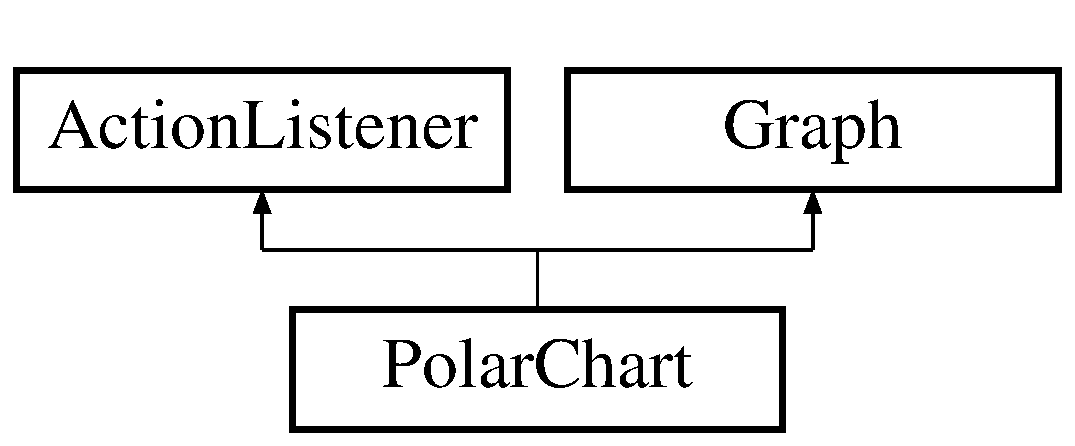
\includegraphics[height=2.000000cm]{class_polar_chart}
\end{center}
\end{figure}
\subsection*{Public Member Functions}
\begin{DoxyCompactItemize}
\item 
\hyperlink{class_polar_chart_a5f108692551cb8c74b55fae0138cc2fb}{Polar\-Chart} (String\mbox{[}$\,$\mbox{]}\mbox{[}$\,$\mbox{]} data, \hyperlink{class_dataset}{Dataset} dataset, \hyperlink{class_data_attribute}{Data\-Attribute} setting)
\item 
\hyperlink{class_polar_chart_a66861893d4eabbb0f8ab27988ce04e86}{Polar\-Chart} (String\mbox{[}$\,$\mbox{]}\mbox{[}$\,$\mbox{]} data, \hyperlink{class_dataset}{Dataset} dataset, \hyperlink{class_data_attribute}{Data\-Attribute} setting, String\mbox{[}$\,$\mbox{]}\mbox{[}$\,$\mbox{]} second\-Data, \hyperlink{class_dataset}{Dataset} second\-Dataset, \hyperlink{class_data_attribute}{Data\-Attribute} second\-Setting)
\item 
\hyperlink{class_polar_chart_a96a2e0f5e310b4982c03d01f65804d7e}{Polar\-Chart} (\hyperlink{class_data_attribute}{Data\-Attribute} setting)
\item 
\hyperlink{class_polar_chart_aba50c5e55fd2d54e6fbdc684724d7d31}{Polar\-Chart} (\hyperlink{class_data_attribute}{Data\-Attribute} setting, \hyperlink{class_data_attribute}{Data\-Attribute} second\-Setting)
\item 
void \hyperlink{class_polar_chart_a9aadea04bcb9d3419f025dbecc8b18f1}{action\-Performed} (Action\-Event e)
\item 
String \hyperlink{class_polar_chart_a2509add6b1beaf9d1c07603dff1b5602}{Set\-Label\-X} (String m\-\_\-x\-Label)
\item 
String \hyperlink{class_polar_chart_a625a4bf978d88a6b2accfd1a7b00fcb0}{Set\-Label\-Y} (String m\-\_\-y\-Label)
\item 
String \hyperlink{class_polar_chart_a1db3b5708bc341845d92584c28c59d34}{Set\-Title} (String m\-\_\-graph\-Title)
\end{DoxyCompactItemize}
\subsection*{Static Public Member Functions}
\begin{DoxyCompactItemize}
\item 
static void \hyperlink{class_polar_chart_a01960911aea80dff1e6872504524e797}{main} (String\mbox{[}$\,$\mbox{]} args)
\end{DoxyCompactItemize}


\subsection{Detailed Description}
A class that creates a single Polar \hyperlink{interface_chart}{Chart} or two Polar \hyperlink{interface_chart}{Chart} visualisations from 2\-D Arrays of data \textbackslash{} see \hyperlink{_graph_8java}{Graph.\-java}. 

\begin{DoxyDate}{Date}
14/04/13 
\end{DoxyDate}
\begin{DoxySeeAlso}{See Also}
This class is responsible for making the Polar chart It was made using J\-Free\-Chart and following examples on how to set up the Polar chart It uses the \hyperlink{_graph_8java}{Graph.\-java} to return a J\-Free\-Chart 
\end{DoxySeeAlso}


\subsection{Constructor \& Destructor Documentation}
\hypertarget{class_polar_chart_a5f108692551cb8c74b55fae0138cc2fb}{\index{Polar\-Chart@{Polar\-Chart}!Polar\-Chart@{Polar\-Chart}}
\index{Polar\-Chart@{Polar\-Chart}!PolarChart@{Polar\-Chart}}
\subsubsection[{Polar\-Chart}]{\setlength{\rightskip}{0pt plus 5cm}Polar\-Chart.\-Polar\-Chart (
\begin{DoxyParamCaption}
\item[{String}]{data\mbox{[}$\,$\mbox{]}\mbox{[}$\,$\mbox{]}, }
\item[{{\bf Dataset}}]{dataset, }
\item[{{\bf Data\-Attribute}}]{setting}
\end{DoxyParamCaption}
)}}\label{class_polar_chart_a5f108692551cb8c74b55fae0138cc2fb}
creates a constructor taking in the following parameters\-:


\begin{DoxyParams}{Parameters}
{\em String\mbox{[}$\,$\mbox{]}\mbox{[}$\,$\mbox{]}} & data -\/ data used to create the visualisation. \\
\hline
{\em \hyperlink{class_dataset}{Dataset}} & dataset -\/ the dataset used (rows and columns) \\
\hline
{\em \hyperlink{class_data_attribute}{Data\-Attribute}} & setting -\/ Data attributes \\
\hline
\end{DoxyParams}

\begin{DoxyCode}
51                                                    \{
52             
53             m\_Data = data;
54             m\_ChartTitle = setting.\hyperlink{class_data_attribute_ade9747a192ba22fe1020e874bff6a48c}{GetTitle}();
55             m\_Setting = setting;
56             m\_XLabel = setting.\hyperlink{class_data_attribute_aecb451704a87d77dd80dbad8a19099d1}{GetAxisLabelX}();
57             m\_YLabel = setting.\hyperlink{class_data_attribute_af5f68794cd0195d42135d5e48120ccc0}{GetAxisLabelY}();
58             m\_Col = dataset.\hyperlink{class_dataset_ab922bef50c8aa1531de8704731779246}{GetNoOfCols}();
59             m\_Row = dataset.\hyperlink{class_dataset_a91257a605317576e87e1c32e54739e51}{GetNoOfRows}();
60             m\_C1 = setting.\hyperlink{class_data_attribute_a0f4a54973bc44b0526f78bda945dc81b}{GetSelectedXIndex}();
61             m\_C2 = setting.\hyperlink{class_data_attribute_a82e7519853d9f470ea183dd0c39a03d6}{GetSelectedYIndex}();
62             
63             CreateDataset(m\_Data);
64             ShowChart(m\_Dataset);
65         \}  
\end{DoxyCode}
\hypertarget{class_polar_chart_a66861893d4eabbb0f8ab27988ce04e86}{\index{Polar\-Chart@{Polar\-Chart}!Polar\-Chart@{Polar\-Chart}}
\index{Polar\-Chart@{Polar\-Chart}!PolarChart@{Polar\-Chart}}
\subsubsection[{Polar\-Chart}]{\setlength{\rightskip}{0pt plus 5cm}Polar\-Chart.\-Polar\-Chart (
\begin{DoxyParamCaption}
\item[{String}]{data\mbox{[}$\,$\mbox{]}\mbox{[}$\,$\mbox{]}, }
\item[{{\bf Dataset}}]{dataset, }
\item[{{\bf Data\-Attribute}}]{setting, }
\item[{String}]{second\-Data\mbox{[}$\,$\mbox{]}\mbox{[}$\,$\mbox{]}, }
\item[{{\bf Dataset}}]{second\-Dataset, }
\item[{{\bf Data\-Attribute}}]{second\-Setting}
\end{DoxyParamCaption}
)}}\label{class_polar_chart_a66861893d4eabbb0f8ab27988ce04e86}
creates a constructor taking in the following parameters\-:


\begin{DoxyParams}{Parameters}
{\em String\mbox{[}$\,$\mbox{]}\mbox{[}$\,$\mbox{]}} & data -\/ data used to create the visualisation. \\
\hline
{\em \hyperlink{class_dataset}{Dataset}} & dataset -\/ the dataset used (rows and columns) \\
\hline
{\em \hyperlink{class_data_attribute}{Data\-Attribute}} & setting -\/ Data attributes \\
\hline
{\em String\mbox{[}$\,$\mbox{]}\mbox{[}$\,$\mbox{]}} & second\-Data -\/ second data used to create the visualisation. \\
\hline
{\em \hyperlink{class_dataset}{Dataset}} & second\-Dataset -\/ the second dataset used (rows and columns) \\
\hline
{\em \hyperlink{class_data_attribute}{Data\-Attribute}} & second\-Setting -\/ Second Data attributes \\
\hline
\end{DoxyParams}

\begin{DoxyCode}
78                                              \{
79             m\_Data = data;
80             m\_SecondData = secondData;
81             m\_Setting = setting;
82             m\_SecondSetting = secondSetting;
83             m\_ChartTitle = setting.\hyperlink{class_data_attribute_ade9747a192ba22fe1020e874bff6a48c}{GetTitle}();
84             m\_SecondChartTitle = secondSetting.\hyperlink{class_data_attribute_a4079522c93025fce7569eaed585f4aeb}{GetSecondTitle}();
85             m\_XLabel = setting.\hyperlink{class_data_attribute_aecb451704a87d77dd80dbad8a19099d1}{GetAxisLabelX}();
86             m\_SecondXLabel = secondSetting.\hyperlink{class_data_attribute_a8ace4cb1fee9e2abeabe3efc9a190c8f}{GetSecondAxisLabelX}();
87             m\_YLabel = setting.\hyperlink{class_data_attribute_af5f68794cd0195d42135d5e48120ccc0}{GetAxisLabelY}();
88             m\_SecondYLabel = secondSetting.\hyperlink{class_data_attribute_a6efb7e067317898feefbbf6bd472b998}{GetSecondAxisLabelY}();
89             m\_Col = dataset.\hyperlink{class_dataset_ab922bef50c8aa1531de8704731779246}{GetNoOfCols}();
90             m\_SecondCol = secondDataset.\hyperlink{class_dataset_ab922bef50c8aa1531de8704731779246}{GetNoOfCols}();
91             m\_Row = dataset.\hyperlink{class_dataset_a91257a605317576e87e1c32e54739e51}{GetNoOfRows}();
92             m\_SecondRow = secondDataset.\hyperlink{class_dataset_a91257a605317576e87e1c32e54739e51}{GetNoOfRows}();
93             m\_C1 = setting.\hyperlink{class_data_attribute_a0f4a54973bc44b0526f78bda945dc81b}{GetSelectedXIndex}();
94             m\_SecondC1 = secondSetting.\hyperlink{class_data_attribute_a7f501790eee650ddf9ac17c4f63a3995}{GetSecondSelectedXIndex}();
95             m\_C2 = setting.\hyperlink{class_data_attribute_a82e7519853d9f470ea183dd0c39a03d6}{GetSelectedYIndex}();
96             m\_SecondC2 = secondSetting.\hyperlink{class_data_attribute_a6f61ad05915f4aa31ad3dba00596da64}{GetSecondSelectedYIndex}();
97              
98              CreateDataset(m\_Data);
99              CreateSecondDataset(m\_SecondData);
100              ShowChart(m\_Dataset, m\_SecondDataset);
101         \}  
\end{DoxyCode}
\hypertarget{class_polar_chart_a96a2e0f5e310b4982c03d01f65804d7e}{\index{Polar\-Chart@{Polar\-Chart}!Polar\-Chart@{Polar\-Chart}}
\index{Polar\-Chart@{Polar\-Chart}!PolarChart@{Polar\-Chart}}
\subsubsection[{Polar\-Chart}]{\setlength{\rightskip}{0pt plus 5cm}Polar\-Chart.\-Polar\-Chart (
\begin{DoxyParamCaption}
\item[{{\bf Data\-Attribute}}]{setting}
\end{DoxyParamCaption}
)}}\label{class_polar_chart_a96a2e0f5e310b4982c03d01f65804d7e}
constructor for J\-Unit Tests 
\begin{DoxyCode}
106                                                   \{
107              m\_ChartTitle = setting.\hyperlink{class_data_attribute_ade9747a192ba22fe1020e874bff6a48c}{GetTitle}();
108              m\_Setting = setting;
109              m\_XLabel = setting.\hyperlink{class_data_attribute_aecb451704a87d77dd80dbad8a19099d1}{GetAxisLabelX}();
110              m\_YLabel = setting.\hyperlink{class_data_attribute_af5f68794cd0195d42135d5e48120ccc0}{GetAxisLabelY}();
111              m\_C1 = setting.\hyperlink{class_data_attribute_a0f4a54973bc44b0526f78bda945dc81b}{GetSelectedXIndex}();
112              m\_C2 = setting.\hyperlink{class_data_attribute_a82e7519853d9f470ea183dd0c39a03d6}{GetSelectedYIndex}();
113             
114         \}
\end{DoxyCode}
\hypertarget{class_polar_chart_aba50c5e55fd2d54e6fbdc684724d7d31}{\index{Polar\-Chart@{Polar\-Chart}!Polar\-Chart@{Polar\-Chart}}
\index{Polar\-Chart@{Polar\-Chart}!PolarChart@{Polar\-Chart}}
\subsubsection[{Polar\-Chart}]{\setlength{\rightskip}{0pt plus 5cm}Polar\-Chart.\-Polar\-Chart (
\begin{DoxyParamCaption}
\item[{{\bf Data\-Attribute}}]{setting, }
\item[{{\bf Data\-Attribute}}]{second\-Setting}
\end{DoxyParamCaption}
)}}\label{class_polar_chart_aba50c5e55fd2d54e6fbdc684724d7d31}
second constructor for J\-Unit Tests 
\begin{DoxyCode}
118                                                                                \{
119              m\_ChartTitle = setting.\hyperlink{class_data_attribute_ade9747a192ba22fe1020e874bff6a48c}{GetTitle}();
120              m\_Setting = setting;
121              m\_XLabel = setting.\hyperlink{class_data_attribute_aecb451704a87d77dd80dbad8a19099d1}{GetAxisLabelX}();
122              m\_YLabel = setting.\hyperlink{class_data_attribute_af5f68794cd0195d42135d5e48120ccc0}{GetAxisLabelY}();
123              m\_C1 = setting.\hyperlink{class_data_attribute_a0f4a54973bc44b0526f78bda945dc81b}{GetSelectedXIndex}();
124              m\_C2 = setting.\hyperlink{class_data_attribute_a82e7519853d9f470ea183dd0c39a03d6}{GetSelectedYIndex}();
125              
126              m\_SecondChartTitle = secondSetting.\hyperlink{class_data_attribute_a4079522c93025fce7569eaed585f4aeb}{GetSecondTitle}();
127              m\_SecondSetting = secondSetting;
128              m\_SecondXLabel = secondSetting.\hyperlink{class_data_attribute_a8ace4cb1fee9e2abeabe3efc9a190c8f}{GetSecondAxisLabelX}();
129              m\_SecondYLabel = secondSetting.\hyperlink{class_data_attribute_a6efb7e067317898feefbbf6bd472b998}{GetSecondAxisLabelY}();
130              m\_SecondC1 = secondSetting.\hyperlink{class_data_attribute_a7f501790eee650ddf9ac17c4f63a3995}{GetSecondSelectedXIndex}();
131              m\_SecondC2 = secondSetting.\hyperlink{class_data_attribute_a6f61ad05915f4aa31ad3dba00596da64}{GetSecondSelectedYIndex}();
132             
133         \}
\end{DoxyCode}


\subsection{Member Function Documentation}
\hypertarget{class_polar_chart_a9aadea04bcb9d3419f025dbecc8b18f1}{\index{Polar\-Chart@{Polar\-Chart}!action\-Performed@{action\-Performed}}
\index{action\-Performed@{action\-Performed}!PolarChart@{Polar\-Chart}}
\subsubsection[{action\-Performed}]{\setlength{\rightskip}{0pt plus 5cm}void Polar\-Chart.\-action\-Performed (
\begin{DoxyParamCaption}
\item[{Action\-Event}]{e}
\end{DoxyParamCaption}
)}}\label{class_polar_chart_a9aadea04bcb9d3419f025dbecc8b18f1}
allows user to select the colour of the points on the Polar chart 
\begin{DoxyCode}
138                                                      \{
139             \textcolor{keywordflow}{if}( e.getSource() == m\_ColChangeButton ) \{
140                 \hyperlink{class_colour_map}{ColourMap} cM = \textcolor{keyword}{new} \hyperlink{class_colour_map}{ColourMap}();
141                 cM.\hyperlink{class_colour_map_a9f696ea699b7fc471bb2dde6f1d1ce09}{SetupData}( m\_Plot.getSeriesCount(), 
142                               m\_Renderer );
143                 cM.setVisible( \textcolor{keyword}{false} );
144             \}
145         \}
\end{DoxyCode}
\hypertarget{class_polar_chart_a01960911aea80dff1e6872504524e797}{\index{Polar\-Chart@{Polar\-Chart}!main@{main}}
\index{main@{main}!PolarChart@{Polar\-Chart}}
\subsubsection[{main}]{\setlength{\rightskip}{0pt plus 5cm}static void Polar\-Chart.\-main (
\begin{DoxyParamCaption}
\item[{String\mbox{[}$\,$\mbox{]}}]{args}
\end{DoxyParamCaption}
)\hspace{0.3cm}{\ttfamily [static]}}}\label{class_polar_chart_a01960911aea80dff1e6872504524e797}
main method to carry out J\-Unit Tests 
\begin{DoxyCode}
337                                                  \{
338             
339             Random generator = \textcolor{keyword}{new} Random();
340             \textcolor{comment}{// Test to display a single chart}
341             XYSeriesCollection testCollection = \textcolor{keyword}{new} XYSeriesCollection();
342             XYSeries testDataset = \textcolor{keyword}{new} XYSeries(\textcolor{stringliteral}{"Test Series"});
343             
344             \hyperlink{class_data_attribute}{DataAttribute} test = \hyperlink{class_data_attribute}{DataAttribute}.
      \hyperlink{class_data_attribute_a9c7a1923698c1530fa38c959596199bc}{GetTestDataAttribute}();
345             \hyperlink{class_polar_chart}{PolarChart} polarChartTest = \textcolor{keyword}{new} \hyperlink{class_polar_chart_a5f108692551cb8c74b55fae0138cc2fb}{PolarChart}(test);
346             
347             \textcolor{keywordflow}{for}(\textcolor{keywordtype}{int} i = 0;i< LOOP;i++) \{
348                 \textcolor{keywordtype}{int} temp1 = generator.nextInt(LIMIT);
349                 \textcolor{keywordtype}{int} temp2 = generator.nextInt(LIMIT);
350                 
351                 testDataset.add(temp1,temp2);
352             \}
353             testCollection.addSeries(testDataset);
354             polarChartTest.ShowChart(testCollection);
355             
356             \textcolor{comment}{// Test to display two charts}
357             XYSeriesCollection secondTestCollection = \textcolor{keyword}{new} XYSeriesCollection();
358             XYSeries secondTestDataset = \textcolor{keyword}{new} XYSeries(\textcolor{stringliteral}{"Second Test Series"});
359             
360             \hyperlink{class_data_attribute}{DataAttribute} secondTest = \hyperlink{class_data_attribute}{DataAttribute}.
      \hyperlink{class_data_attribute_a9c7a1923698c1530fa38c959596199bc}{GetTestDataAttribute}();
361             \hyperlink{class_polar_chart}{PolarChart} secondPolarChartTest = \textcolor{keyword}{new} \hyperlink{class_polar_chart_a5f108692551cb8c74b55fae0138cc2fb}{PolarChart}(secondTest);
362             
363             \textcolor{keywordflow}{for}(\textcolor{keywordtype}{int} i = 0;i< LOOP;i++) \{
364                 \textcolor{keywordtype}{int} temp1 = generator.nextInt(LIMIT);
365                 \textcolor{keywordtype}{int} temp2 = generator.nextInt(LIMIT);
366                 
367                 secondTestDataset.add(temp1,temp2);
368             \}
369             secondTestCollection.addSeries(secondTestDataset);
370             secondPolarChartTest.ShowChart(testCollection,secondTestCollection);
371         
372         
373         \}
\end{DoxyCode}
\hypertarget{class_polar_chart_a2509add6b1beaf9d1c07603dff1b5602}{\index{Polar\-Chart@{Polar\-Chart}!Set\-Label\-X@{Set\-Label\-X}}
\index{Set\-Label\-X@{Set\-Label\-X}!PolarChart@{Polar\-Chart}}
\subsubsection[{Set\-Label\-X}]{\setlength{\rightskip}{0pt plus 5cm}String Polar\-Chart.\-Set\-Label\-X (
\begin{DoxyParamCaption}
\item[{String}]{m\-\_\-x\-Label}
\end{DoxyParamCaption}
)}}\label{class_polar_chart_a2509add6b1beaf9d1c07603dff1b5602}

\begin{DoxyParams}{Parameters}
{\em m\-\_\-x\-Label} & -\/ the x axis label passed from users to the graph \\
\hline
\end{DoxyParams}
\begin{DoxyReturn}{Returns}
m\-\_\-label\-X -\/ returns the user's x label value 
\end{DoxyReturn}

\begin{DoxyCode}
152                                                    \{
153             String m\_labelX = m\_xLabel;
154             \textcolor{keywordflow}{return} m\_labelX;
155         \}
\end{DoxyCode}
\hypertarget{class_polar_chart_a625a4bf978d88a6b2accfd1a7b00fcb0}{\index{Polar\-Chart@{Polar\-Chart}!Set\-Label\-Y@{Set\-Label\-Y}}
\index{Set\-Label\-Y@{Set\-Label\-Y}!PolarChart@{Polar\-Chart}}
\subsubsection[{Set\-Label\-Y}]{\setlength{\rightskip}{0pt plus 5cm}String Polar\-Chart.\-Set\-Label\-Y (
\begin{DoxyParamCaption}
\item[{String}]{m\-\_\-y\-Label}
\end{DoxyParamCaption}
)}}\label{class_polar_chart_a625a4bf978d88a6b2accfd1a7b00fcb0}

\begin{DoxyParams}{Parameters}
{\em m\-\_\-y\-Label} & -\/ the y axis label passed from users to the graph \\
\hline
\end{DoxyParams}
\begin{DoxyReturn}{Returns}
m\-\_\-label\-Y -\/ returns the user's y label value 
\end{DoxyReturn}

\begin{DoxyCode}
162                                                    \{
163             String m\_labelY = m\_yLabel;
164             \textcolor{keywordflow}{return} m\_labelY;
165         \}
\end{DoxyCode}
\hypertarget{class_polar_chart_a1db3b5708bc341845d92584c28c59d34}{\index{Polar\-Chart@{Polar\-Chart}!Set\-Title@{Set\-Title}}
\index{Set\-Title@{Set\-Title}!PolarChart@{Polar\-Chart}}
\subsubsection[{Set\-Title}]{\setlength{\rightskip}{0pt plus 5cm}String Polar\-Chart.\-Set\-Title (
\begin{DoxyParamCaption}
\item[{String}]{m\-\_\-graph\-Title}
\end{DoxyParamCaption}
)}}\label{class_polar_chart_a1db3b5708bc341845d92584c28c59d34}

\begin{DoxyParams}{Parameters}
{\em m\-\_\-graph\-Title} & -\/ the title passed from users to the graph \\
\hline
\end{DoxyParams}
\begin{DoxyReturn}{Returns}
m\-\_\-title -\/ returns the user's title value 
\end{DoxyReturn}

\begin{DoxyCode}
172                                                       \{
173             String m\_title = m\_graphTitle;
174             \textcolor{keywordflow}{return} m\_title;
175         \} 
\end{DoxyCode}


The documentation for this class was generated from the following file\-:\begin{DoxyCompactItemize}
\item 
\hyperlink{_polar_chart_8java}{Polar\-Chart.\-java}\end{DoxyCompactItemize}

\hypertarget{class_scatter_plot_graph}{\section{Scatter\-Plot\-Graph Class Reference}
\label{class_scatter_plot_graph}\index{Scatter\-Plot\-Graph@{Scatter\-Plot\-Graph}}
}


A class that creates a single Scatter Plot \hyperlink{interface_graph}{Graph} or two Scatter Plot \hyperlink{interface_graph}{Graph} visualisations from a 2\-D Array of data.  


Inheritance diagram for Scatter\-Plot\-Graph\-:\begin{figure}[H]
\begin{center}
\leavevmode
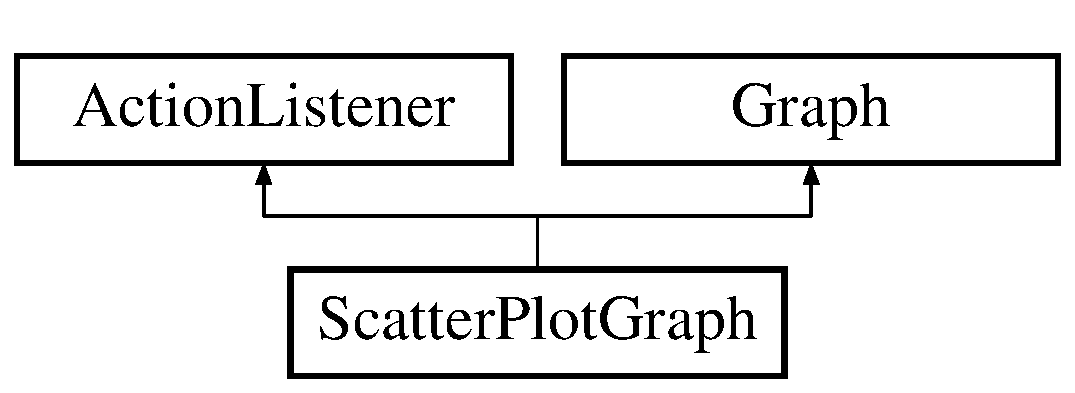
\includegraphics[height=2.000000cm]{class_scatter_plot_graph}
\end{center}
\end{figure}
\subsection*{Public Member Functions}
\begin{DoxyCompactItemize}
\item 
\hyperlink{class_scatter_plot_graph_ac2fd61853bd154841052c26cb3ffb4be}{Scatter\-Plot\-Graph} (String\mbox{[}$\,$\mbox{]}\mbox{[}$\,$\mbox{]} data, \hyperlink{class_dataset}{Dataset} dataset, \hyperlink{class_data_attribute}{Data\-Attribute} setting)
\item 
\hyperlink{class_scatter_plot_graph_a7ef427d6eaea9bd50ac1e3b489ab475e}{Scatter\-Plot\-Graph} (String\mbox{[}$\,$\mbox{]}\mbox{[}$\,$\mbox{]} data, \hyperlink{class_dataset}{Dataset} dataset, \hyperlink{class_data_attribute}{Data\-Attribute} setting, String\mbox{[}$\,$\mbox{]}\mbox{[}$\,$\mbox{]} second\-Data, \hyperlink{class_dataset}{Dataset} second\-Dataset, \hyperlink{class_data_attribute}{Data\-Attribute} second\-Setting)
\item 
\hyperlink{class_scatter_plot_graph_afb2052a677d1caa6fee0897e57f3f964}{Scatter\-Plot\-Graph} (\hyperlink{class_data_attribute}{Data\-Attribute} setting)
\item 
\hyperlink{class_scatter_plot_graph_a654a461323b804f56e918359fd53895d}{Scatter\-Plot\-Graph} (\hyperlink{class_data_attribute}{Data\-Attribute} setting, \hyperlink{class_data_attribute}{Data\-Attribute} second\-Setting)
\item 
\hyperlink{class_scatter_plot_graph_a41ca56e8fb709cf0339e1b3cb46ace51}{Scatter\-Plot\-Graph} ()
\item 
void \hyperlink{class_scatter_plot_graph_aebbb9e7e1bab5bebfa9dacdb3c1f33cb}{action\-Performed} (Action\-Event e)
\item 
String \hyperlink{class_scatter_plot_graph_a5c475561f712ff1f59a394f799d90bc1}{Set\-Label\-X} (String m\-\_\-x\-Label)
\item 
String \hyperlink{class_scatter_plot_graph_a3f1b7d2f08c25432395a50c4c3bd3101}{Set\-Label\-Y} (String m\-\_\-y\-Label)
\item 
String \hyperlink{class_scatter_plot_graph_a4d6cbf2ae379db2d6e0e06a1ffb868ca}{Set\-Title} (String m\-\_\-graph\-Title)
\end{DoxyCompactItemize}
\subsection*{Static Public Member Functions}
\begin{DoxyCompactItemize}
\item 
static void \hyperlink{class_scatter_plot_graph_a9579fc0c252b63f71e608c69c4057bd0}{main} (String\mbox{[}$\,$\mbox{]} args)
\end{DoxyCompactItemize}


\subsection{Detailed Description}
A class that creates a single Scatter Plot \hyperlink{interface_graph}{Graph} or two Scatter Plot \hyperlink{interface_graph}{Graph} visualisations from a 2\-D Array of data. 

\begin{DoxyDate}{Date}
30/04/13 
\end{DoxyDate}
\begin{DoxySeeAlso}{See Also}

\end{DoxySeeAlso}


\subsection{Constructor \& Destructor Documentation}
\hypertarget{class_scatter_plot_graph_ac2fd61853bd154841052c26cb3ffb4be}{\index{Scatter\-Plot\-Graph@{Scatter\-Plot\-Graph}!Scatter\-Plot\-Graph@{Scatter\-Plot\-Graph}}
\index{Scatter\-Plot\-Graph@{Scatter\-Plot\-Graph}!ScatterPlotGraph@{Scatter\-Plot\-Graph}}
\subsubsection[{Scatter\-Plot\-Graph}]{\setlength{\rightskip}{0pt plus 5cm}Scatter\-Plot\-Graph.\-Scatter\-Plot\-Graph (
\begin{DoxyParamCaption}
\item[{String}]{data\mbox{[}$\,$\mbox{]}\mbox{[}$\,$\mbox{]}, }
\item[{{\bf Dataset}}]{dataset, }
\item[{{\bf Data\-Attribute}}]{setting}
\end{DoxyParamCaption}
)}}\label{class_scatter_plot_graph_ac2fd61853bd154841052c26cb3ffb4be}
creates a constructor taking in the following parameters\-:


\begin{DoxyParams}{Parameters}
{\em String\mbox{[}$\,$\mbox{]}\mbox{[}$\,$\mbox{]}} & data -\/ data used to create the visualisation. \\
\hline
{\em \hyperlink{class_dataset}{Dataset}} & dataset -\/ the dataset used (rows and columns) \\
\hline
{\em \hyperlink{class_data_attribute}{Data\-Attribute}} & setting -\/ Data attributes \\
\hline
\end{DoxyParams}

\begin{DoxyCode}
43                                                       \{
44         
45         m\_Data = data;
46         m\_Setting = setting;
47         m\_ChartTitle = setting.\hyperlink{class_data_attribute_ade9747a192ba22fe1020e874bff6a48c}{GetTitle}();
48         m\_XLabel = setting.\hyperlink{class_data_attribute_aecb451704a87d77dd80dbad8a19099d1}{GetAxisLabelX}();
49         m\_YLabel = setting.\hyperlink{class_data_attribute_af5f68794cd0195d42135d5e48120ccc0}{GetAxisLabelY}();
50         m\_Col = dataset.\hyperlink{class_dataset_ab922bef50c8aa1531de8704731779246}{GetNoOfCols}();
51         m\_Row = dataset.\hyperlink{class_dataset_a91257a605317576e87e1c32e54739e51}{GetNoOfRows}();
52         m\_C1 = setting.\hyperlink{class_data_attribute_a0f4a54973bc44b0526f78bda945dc81b}{GetSelectedXIndex}();
53         m\_C2 = setting.\hyperlink{class_data_attribute_a82e7519853d9f470ea183dd0c39a03d6}{GetSelectedYIndex}();
54         
55         m\_XMin = setting.\hyperlink{class_data_attribute_afa9da883abc4abad5f64c045de114c50}{GetXAxisMin}();
56         m\_XMax = setting.\hyperlink{class_data_attribute_a81243eb8f7008e05e74b0f3571d2f08d}{GetYAxisMax}();
57         m\_XScale = setting.\hyperlink{class_data_attribute_a5a1de25600487aa958a19ce01151fea4}{GetXAxisScale}();
58         m\_YScale = setting.\hyperlink{class_data_attribute_a95259727ce91efc0e0eaa28487d944c5}{GetYAxisScale}();
59         
60         createDataset( m\_Data );
61         showGraph( m\_Dataset );
62     \}  
\end{DoxyCode}
\hypertarget{class_scatter_plot_graph_a7ef427d6eaea9bd50ac1e3b489ab475e}{\index{Scatter\-Plot\-Graph@{Scatter\-Plot\-Graph}!Scatter\-Plot\-Graph@{Scatter\-Plot\-Graph}}
\index{Scatter\-Plot\-Graph@{Scatter\-Plot\-Graph}!ScatterPlotGraph@{Scatter\-Plot\-Graph}}
\subsubsection[{Scatter\-Plot\-Graph}]{\setlength{\rightskip}{0pt plus 5cm}Scatter\-Plot\-Graph.\-Scatter\-Plot\-Graph (
\begin{DoxyParamCaption}
\item[{String}]{data\mbox{[}$\,$\mbox{]}\mbox{[}$\,$\mbox{]}, }
\item[{{\bf Dataset}}]{dataset, }
\item[{{\bf Data\-Attribute}}]{setting, }
\item[{String}]{second\-Data\mbox{[}$\,$\mbox{]}\mbox{[}$\,$\mbox{]}, }
\item[{{\bf Dataset}}]{second\-Dataset, }
\item[{{\bf Data\-Attribute}}]{second\-Setting}
\end{DoxyParamCaption}
)}}\label{class_scatter_plot_graph_a7ef427d6eaea9bd50ac1e3b489ab475e}
creates a constructor taking in the following parameters\-:


\begin{DoxyParams}{Parameters}
{\em String\mbox{[}$\,$\mbox{]}\mbox{[}$\,$\mbox{]}} & data -\/ data used to create the visualisation. \\
\hline
{\em \hyperlink{class_dataset}{Dataset}} & dataset -\/ the dataset used (rows and columns) \\
\hline
{\em \hyperlink{class_data_attribute}{Data\-Attribute}} & setting -\/ Data attributes \\
\hline
{\em String\mbox{[}$\,$\mbox{]}\mbox{[}$\,$\mbox{]}} & second\-Data -\/ second data used to create the visualisation. \\
\hline
{\em \hyperlink{class_dataset}{Dataset}} & second\-Dataset -\/ the second dataset used (rows and columns) \\
\hline
{\em \hyperlink{class_data_attribute}{Data\-Attribute}} & second\-Setting -\/ Second Data attributes \\
\hline
\end{DoxyParams}

\begin{DoxyCode}
75                                          \{
76 
77         m\_Data = data;
78         m\_SecondData = secondData;
79         m\_Setting = setting;
80         m\_SecondSetting = secondSetting;
81         m\_ChartTitle = setting.\hyperlink{class_data_attribute_ade9747a192ba22fe1020e874bff6a48c}{GetTitle}();
82         m\_SecondChartTitle = secondSetting.\hyperlink{class_data_attribute_a4079522c93025fce7569eaed585f4aeb}{GetSecondTitle}();
83         m\_XLabel = setting.\hyperlink{class_data_attribute_aecb451704a87d77dd80dbad8a19099d1}{GetAxisLabelX}();
84         m\_SecondXLabel = secondSetting.\hyperlink{class_data_attribute_a8ace4cb1fee9e2abeabe3efc9a190c8f}{GetSecondAxisLabelX}();
85         m\_YLabel = setting.\hyperlink{class_data_attribute_af5f68794cd0195d42135d5e48120ccc0}{GetAxisLabelY}();
86         m\_SecondYLabel = secondSetting.\hyperlink{class_data_attribute_a6efb7e067317898feefbbf6bd472b998}{GetSecondAxisLabelY}();
87         m\_Col = dataset.\hyperlink{class_dataset_ab922bef50c8aa1531de8704731779246}{GetNoOfCols}();
88         m\_SecondCol = secondDataset.\hyperlink{class_dataset_ab922bef50c8aa1531de8704731779246}{GetNoOfCols}();
89         m\_Row = dataset.\hyperlink{class_dataset_a91257a605317576e87e1c32e54739e51}{GetNoOfRows}();
90         m\_SecondRow = secondDataset.\hyperlink{class_dataset_a91257a605317576e87e1c32e54739e51}{GetNoOfRows}();
91         m\_C1 = setting.\hyperlink{class_data_attribute_a0f4a54973bc44b0526f78bda945dc81b}{GetSelectedXIndex}();
92         m\_SecondC1 = secondSetting.\hyperlink{class_data_attribute_a7f501790eee650ddf9ac17c4f63a3995}{GetSecondSelectedXIndex}();
93         m\_C2 = setting.\hyperlink{class_data_attribute_a82e7519853d9f470ea183dd0c39a03d6}{GetSelectedYIndex}();
94         m\_SecondC2 = secondSetting.\hyperlink{class_data_attribute_a6f61ad05915f4aa31ad3dba00596da64}{GetSecondSelectedYIndex}();
95         
96         m\_XMin = setting.\hyperlink{class_data_attribute_afa9da883abc4abad5f64c045de114c50}{GetXAxisMin}();
97         m\_XMax = setting.\hyperlink{class_data_attribute_a81243eb8f7008e05e74b0f3571d2f08d}{GetYAxisMax}();
98         m\_XScale = setting.\hyperlink{class_data_attribute_a5a1de25600487aa958a19ce01151fea4}{GetXAxisScale}();
99         m\_YScale = setting.\hyperlink{class_data_attribute_a95259727ce91efc0e0eaa28487d944c5}{GetYAxisScale}();
100 
101         m\_SecondXMin = secondSetting.\hyperlink{class_data_attribute_afa9da883abc4abad5f64c045de114c50}{GetXAxisMin}();
102         m\_SecondXMax = secondSetting.\hyperlink{class_data_attribute_a81243eb8f7008e05e74b0f3571d2f08d}{GetYAxisMax}();
103         m\_SecondXScale = secondSetting.\hyperlink{class_data_attribute_a5a1de25600487aa958a19ce01151fea4}{GetXAxisScale}();
104         m\_SecondYScale = secondSetting.\hyperlink{class_data_attribute_a95259727ce91efc0e0eaa28487d944c5}{GetYAxisScale}();
105         
106         createDataset( m\_Data );
107         createSecondDataset(m\_SecondData);
108         showGraph(m\_Dataset, m\_SecondDataset);
109     \}  
\end{DoxyCode}
\hypertarget{class_scatter_plot_graph_afb2052a677d1caa6fee0897e57f3f964}{\index{Scatter\-Plot\-Graph@{Scatter\-Plot\-Graph}!Scatter\-Plot\-Graph@{Scatter\-Plot\-Graph}}
\index{Scatter\-Plot\-Graph@{Scatter\-Plot\-Graph}!ScatterPlotGraph@{Scatter\-Plot\-Graph}}
\subsubsection[{Scatter\-Plot\-Graph}]{\setlength{\rightskip}{0pt plus 5cm}Scatter\-Plot\-Graph.\-Scatter\-Plot\-Graph (
\begin{DoxyParamCaption}
\item[{{\bf Data\-Attribute}}]{setting}
\end{DoxyParamCaption}
)}}\label{class_scatter_plot_graph_afb2052a677d1caa6fee0897e57f3f964}
constructor for J\-Unit Tests 
\begin{DoxyParams}{Parameters}
{\em setting} & \\
\hline
\end{DoxyParams}

\begin{DoxyCode}
114                                                    \{
115         m\_ChartTitle = setting.\hyperlink{class_data_attribute_ade9747a192ba22fe1020e874bff6a48c}{GetTitle}();
116         m\_Setting = setting;
117         m\_XLabel = setting.\hyperlink{class_data_attribute_aecb451704a87d77dd80dbad8a19099d1}{GetAxisLabelX}();
118         m\_YLabel = setting.\hyperlink{class_data_attribute_af5f68794cd0195d42135d5e48120ccc0}{GetAxisLabelY}();
119         m\_C1 = setting.\hyperlink{class_data_attribute_a0f4a54973bc44b0526f78bda945dc81b}{GetSelectedXIndex}();
120         m\_C2 = setting.\hyperlink{class_data_attribute_a82e7519853d9f470ea183dd0c39a03d6}{GetSelectedYIndex}();
121         m\_XMin = setting.\hyperlink{class_data_attribute_afa9da883abc4abad5f64c045de114c50}{GetXAxisMin}();
122         m\_XMax = setting.\hyperlink{class_data_attribute_ada370712422c7cbd21b7be4a0d88caf7}{GetXAxisMax}();
123         m\_YMin = setting.\hyperlink{class_data_attribute_af0786b4de674874c0bb8ca9dbe1519c6}{GetYAxisMin}();
124         m\_YMax = setting.\hyperlink{class_data_attribute_a81243eb8f7008e05e74b0f3571d2f08d}{GetYAxisMax}();
125         m\_XScale = setting.\hyperlink{class_data_attribute_a5a1de25600487aa958a19ce01151fea4}{GetXAxisScale}();
126         m\_YScale = setting.\hyperlink{class_data_attribute_a95259727ce91efc0e0eaa28487d944c5}{GetYAxisScale}();
127     \}
\end{DoxyCode}
\hypertarget{class_scatter_plot_graph_a654a461323b804f56e918359fd53895d}{\index{Scatter\-Plot\-Graph@{Scatter\-Plot\-Graph}!Scatter\-Plot\-Graph@{Scatter\-Plot\-Graph}}
\index{Scatter\-Plot\-Graph@{Scatter\-Plot\-Graph}!ScatterPlotGraph@{Scatter\-Plot\-Graph}}
\subsubsection[{Scatter\-Plot\-Graph}]{\setlength{\rightskip}{0pt plus 5cm}Scatter\-Plot\-Graph.\-Scatter\-Plot\-Graph (
\begin{DoxyParamCaption}
\item[{{\bf Data\-Attribute}}]{setting, }
\item[{{\bf Data\-Attribute}}]{second\-Setting}
\end{DoxyParamCaption}
)}}\label{class_scatter_plot_graph_a654a461323b804f56e918359fd53895d}
second constructor for J\-Unit Tests 
\begin{DoxyParams}{Parameters}
{\em setting} & \\
\hline
\end{DoxyParams}

\begin{DoxyCode}
132                                                                                 \{
133         m\_ChartTitle = setting.\hyperlink{class_data_attribute_ade9747a192ba22fe1020e874bff6a48c}{GetTitle}();
134         m\_Setting = setting;
135         m\_XLabel = setting.\hyperlink{class_data_attribute_aecb451704a87d77dd80dbad8a19099d1}{GetAxisLabelX}();
136         m\_YLabel = setting.\hyperlink{class_data_attribute_af5f68794cd0195d42135d5e48120ccc0}{GetAxisLabelY}();
137         m\_C1 = setting.\hyperlink{class_data_attribute_a0f4a54973bc44b0526f78bda945dc81b}{GetSelectedXIndex}();
138         m\_C2 = setting.\hyperlink{class_data_attribute_a82e7519853d9f470ea183dd0c39a03d6}{GetSelectedYIndex}();
139         m\_XMin = setting.\hyperlink{class_data_attribute_afa9da883abc4abad5f64c045de114c50}{GetXAxisMin}();
140         m\_XMax = setting.\hyperlink{class_data_attribute_ada370712422c7cbd21b7be4a0d88caf7}{GetXAxisMax}();
141         m\_YMin = setting.\hyperlink{class_data_attribute_af0786b4de674874c0bb8ca9dbe1519c6}{GetYAxisMin}();
142         m\_YMax = setting.\hyperlink{class_data_attribute_a81243eb8f7008e05e74b0f3571d2f08d}{GetYAxisMax}();
143         m\_XScale = setting.\hyperlink{class_data_attribute_a5a1de25600487aa958a19ce01151fea4}{GetXAxisScale}();
144         m\_YScale = setting.\hyperlink{class_data_attribute_a95259727ce91efc0e0eaa28487d944c5}{GetYAxisScale}();
145         
146         m\_SecondChartTitle = secondSetting.\hyperlink{class_data_attribute_a4079522c93025fce7569eaed585f4aeb}{GetSecondTitle}();
147         m\_SecondSetting = secondSetting;
148         m\_SecondXLabel = secondSetting.\hyperlink{class_data_attribute_a8ace4cb1fee9e2abeabe3efc9a190c8f}{GetSecondAxisLabelX}();
149         m\_SecondYLabel = secondSetting.\hyperlink{class_data_attribute_a6efb7e067317898feefbbf6bd472b998}{GetSecondAxisLabelY}();
150         m\_SecondC1 = secondSetting.\hyperlink{class_data_attribute_a7f501790eee650ddf9ac17c4f63a3995}{GetSecondSelectedXIndex}();
151         m\_SecondC2 = secondSetting.\hyperlink{class_data_attribute_a6f61ad05915f4aa31ad3dba00596da64}{GetSecondSelectedYIndex}();
152         m\_SecondXMin = secondSetting.\hyperlink{class_data_attribute_afa9da883abc4abad5f64c045de114c50}{GetXAxisMin}();
153         m\_SecondXMax = secondSetting.\hyperlink{class_data_attribute_ada370712422c7cbd21b7be4a0d88caf7}{GetXAxisMax}();
154         m\_SecondYMin = secondSetting.\hyperlink{class_data_attribute_af0786b4de674874c0bb8ca9dbe1519c6}{GetYAxisMin}();
155         m\_SecondYMax = secondSetting.\hyperlink{class_data_attribute_a81243eb8f7008e05e74b0f3571d2f08d}{GetYAxisMax}();
156         m\_SecondXScale = secondSetting.\hyperlink{class_data_attribute_a5a1de25600487aa958a19ce01151fea4}{GetXAxisScale}();
157         m\_SecondYScale = secondSetting.\hyperlink{class_data_attribute_a95259727ce91efc0e0eaa28487d944c5}{GetYAxisScale}();
158     \}
\end{DoxyCode}
\hypertarget{class_scatter_plot_graph_a41ca56e8fb709cf0339e1b3cb46ace51}{\index{Scatter\-Plot\-Graph@{Scatter\-Plot\-Graph}!Scatter\-Plot\-Graph@{Scatter\-Plot\-Graph}}
\index{Scatter\-Plot\-Graph@{Scatter\-Plot\-Graph}!ScatterPlotGraph@{Scatter\-Plot\-Graph}}
\subsubsection[{Scatter\-Plot\-Graph}]{\setlength{\rightskip}{0pt plus 5cm}Scatter\-Plot\-Graph.\-Scatter\-Plot\-Graph (
\begin{DoxyParamCaption}
{}
\end{DoxyParamCaption}
)}}\label{class_scatter_plot_graph_a41ca56e8fb709cf0339e1b3cb46ace51}
second empty constructor for J\-Unit Tests 
\begin{DoxyCode}
163 \{\}
\end{DoxyCode}


\subsection{Member Function Documentation}
\hypertarget{class_scatter_plot_graph_aebbb9e7e1bab5bebfa9dacdb3c1f33cb}{\index{Scatter\-Plot\-Graph@{Scatter\-Plot\-Graph}!action\-Performed@{action\-Performed}}
\index{action\-Performed@{action\-Performed}!ScatterPlotGraph@{Scatter\-Plot\-Graph}}
\subsubsection[{action\-Performed}]{\setlength{\rightskip}{0pt plus 5cm}void Scatter\-Plot\-Graph.\-action\-Performed (
\begin{DoxyParamCaption}
\item[{Action\-Event}]{e}
\end{DoxyParamCaption}
)}}\label{class_scatter_plot_graph_aebbb9e7e1bab5bebfa9dacdb3c1f33cb}
allows user to select the colour of the points on the scatter graph 
\begin{DoxyCode}
169                                                  \{
170         \textcolor{keywordflow}{if}( e.getSource() == m\_ColChangeButton ) \{
171             \hyperlink{class_colour_map}{ColourMap} cM = \textcolor{keyword}{new} \hyperlink{class_colour_map}{ColourMap}();
172             cM.\hyperlink{class_colour_map_a9f696ea699b7fc471bb2dde6f1d1ce09}{SetupData}( m\_Plot.getSeriesCount(), 
173                           m\_Renderer );
174             cM.setVisible( \textcolor{keyword}{false} );
175         \}
176     \}
\end{DoxyCode}
\hypertarget{class_scatter_plot_graph_a9579fc0c252b63f71e608c69c4057bd0}{\index{Scatter\-Plot\-Graph@{Scatter\-Plot\-Graph}!main@{main}}
\index{main@{main}!ScatterPlotGraph@{Scatter\-Plot\-Graph}}
\subsubsection[{main}]{\setlength{\rightskip}{0pt plus 5cm}static void Scatter\-Plot\-Graph.\-main (
\begin{DoxyParamCaption}
\item[{String\mbox{[}$\,$\mbox{]}}]{args}
\end{DoxyParamCaption}
)\hspace{0.3cm}{\ttfamily [static]}}}\label{class_scatter_plot_graph_a9579fc0c252b63f71e608c69c4057bd0}
main method to carry out J\-Unit Tests 
\begin{DoxyCode}
393                                              \{
394          \textcolor{comment}{// Test to display a single chart}
395         \hyperlink{class_data_attribute}{DataAttribute} test = \hyperlink{class_data_attribute}{DataAttribute}.
      \hyperlink{class_data_attribute_a9c7a1923698c1530fa38c959596199bc}{GetTestDataAttribute}();
396         \hyperlink{class_scatter_plot_graph}{ScatterPlotGraph} scatterTest = \textcolor{keyword}{new} \hyperlink{class_scatter_plot_graph_a41ca56e8fb709cf0339e1b3cb46ace51}{ScatterPlotGraph}(test);
397         
398         Random generator = \textcolor{keyword}{new} Random();
399         
400         XYSeriesCollection dataSeries = \textcolor{keyword}{new} XYSeriesCollection();
401         XYSeries dataset = \textcolor{keyword}{new} XYSeries(\textcolor{stringliteral}{"testSeries"}); 
402         \textcolor{keywordflow}{for}(\textcolor{keywordtype}{int} i = 0;i < LOOP;i++) \{
403             \textcolor{keywordtype}{int} temp1 = generator.nextInt();
404             \textcolor{keywordtype}{int} temp2 = generator.nextInt();
405             dataset.add(temp1,temp2);
406         \}
407         dataSeries.addSeries(dataset);
408         
409         scatterTest.showGraph(dataSeries);
410         
411         \textcolor{comment}{// Test to display the two charts}
412         \hyperlink{class_data_attribute}{DataAttribute} firstTest = \hyperlink{class_data_attribute}{DataAttribute}.
      \hyperlink{class_data_attribute_a9c7a1923698c1530fa38c959596199bc}{GetTestDataAttribute}();
413         \hyperlink{class_data_attribute}{DataAttribute} secondTest = \hyperlink{class_data_attribute}{DataAttribute}.
      \hyperlink{class_data_attribute_a9c7a1923698c1530fa38c959596199bc}{GetTestDataAttribute}();
414         
415         XYSeriesCollection secondDataSeries = \textcolor{keyword}{new} XYSeriesCollection();
416         XYSeries secondDataset = \textcolor{keyword}{new} XYSeries(\textcolor{stringliteral}{"testSeries"}); 
417         \textcolor{keywordflow}{for}(\textcolor{keywordtype}{int} i = 0;i < LOOP;i++) \{
418             \textcolor{keywordtype}{int} temp1 = generator.nextInt();
419             \textcolor{keywordtype}{int} temp2 = generator.nextInt();
420             dataset.add(temp1,temp2);
421         \}
422         secondDataSeries.addSeries(dataset);
423         secondDataSeries.addSeries(secondDataset);
424         
425         scatterTest.showGraph(dataSeries, secondDataSeries);
426     \}
\end{DoxyCode}
\hypertarget{class_scatter_plot_graph_a5c475561f712ff1f59a394f799d90bc1}{\index{Scatter\-Plot\-Graph@{Scatter\-Plot\-Graph}!Set\-Label\-X@{Set\-Label\-X}}
\index{Set\-Label\-X@{Set\-Label\-X}!ScatterPlotGraph@{Scatter\-Plot\-Graph}}
\subsubsection[{Set\-Label\-X}]{\setlength{\rightskip}{0pt plus 5cm}String Scatter\-Plot\-Graph.\-Set\-Label\-X (
\begin{DoxyParamCaption}
\item[{String}]{m\-\_\-x\-Label}
\end{DoxyParamCaption}
)}}\label{class_scatter_plot_graph_a5c475561f712ff1f59a394f799d90bc1}

\begin{DoxyParams}{Parameters}
{\em m\-\_\-x\-Label} & -\/ the x axis label passed from users to the graph \\
\hline
\end{DoxyParams}
\begin{DoxyReturn}{Returns}
m\-\_\-label\-X -\/ returns the user's x label value 
\end{DoxyReturn}

\begin{DoxyCode}
183                                                \{
184     String m\_labelX = m\_xLabel;
185         \textcolor{keywordtype}{boolean} test = \textcolor{keyword}{true};                   
186         \textcolor{keywordflow}{return} m\_labelX;
187     \}
\end{DoxyCode}
\hypertarget{class_scatter_plot_graph_a3f1b7d2f08c25432395a50c4c3bd3101}{\index{Scatter\-Plot\-Graph@{Scatter\-Plot\-Graph}!Set\-Label\-Y@{Set\-Label\-Y}}
\index{Set\-Label\-Y@{Set\-Label\-Y}!ScatterPlotGraph@{Scatter\-Plot\-Graph}}
\subsubsection[{Set\-Label\-Y}]{\setlength{\rightskip}{0pt plus 5cm}String Scatter\-Plot\-Graph.\-Set\-Label\-Y (
\begin{DoxyParamCaption}
\item[{String}]{m\-\_\-y\-Label}
\end{DoxyParamCaption}
)}}\label{class_scatter_plot_graph_a3f1b7d2f08c25432395a50c4c3bd3101}

\begin{DoxyParams}{Parameters}
{\em m\-\_\-y\-Label} & -\/ the y axis label passed from users to the graph \\
\hline
\end{DoxyParams}
\begin{DoxyReturn}{Returns}
m\-\_\-label\-Y -\/ returns the user's y label value 
\end{DoxyReturn}

\begin{DoxyCode}
194                                                \{
195         String m\_labelY = m\_yLabel;
196         \textcolor{keywordflow}{return} m\_labelY;
197     \}
\end{DoxyCode}
\hypertarget{class_scatter_plot_graph_a4d6cbf2ae379db2d6e0e06a1ffb868ca}{\index{Scatter\-Plot\-Graph@{Scatter\-Plot\-Graph}!Set\-Title@{Set\-Title}}
\index{Set\-Title@{Set\-Title}!ScatterPlotGraph@{Scatter\-Plot\-Graph}}
\subsubsection[{Set\-Title}]{\setlength{\rightskip}{0pt plus 5cm}String Scatter\-Plot\-Graph.\-Set\-Title (
\begin{DoxyParamCaption}
\item[{String}]{m\-\_\-graph\-Title}
\end{DoxyParamCaption}
)}}\label{class_scatter_plot_graph_a4d6cbf2ae379db2d6e0e06a1ffb868ca}

\begin{DoxyParams}{Parameters}
{\em m\-\_\-graph\-Title} & -\/ the title passed from users to the graph \\
\hline
\end{DoxyParams}
\begin{DoxyReturn}{Returns}
m\-\_\-title -\/ returns the user's title value 
\end{DoxyReturn}

\begin{DoxyCode}
204                                                   \{
205         String m\_title = m\_graphTitle;
206         
207         \textcolor{keywordtype}{boolean} test = \textcolor{keyword}{true};
208         \textcolor{keywordflow}{return} m\_title;
209     \} 
\end{DoxyCode}


The documentation for this class was generated from the following file\-:\begin{DoxyCompactItemize}
\item 
\hyperlink{_scatter_plot_graph_8java}{Scatter\-Plot\-Graph.\-java}\end{DoxyCompactItemize}

\hypertarget{class_selection_viz_j_panel}{\section{Selection\-Viz\-J\-Panel Class Reference}
\label{class_selection_viz_j_panel}\index{Selection\-Viz\-J\-Panel@{Selection\-Viz\-J\-Panel}}
}


This class passes the data from the G\-U\-I to the constructors of the visualisation types.  


Inheritance diagram for Selection\-Viz\-J\-Panel\-:\begin{figure}[H]
\begin{center}
\leavevmode
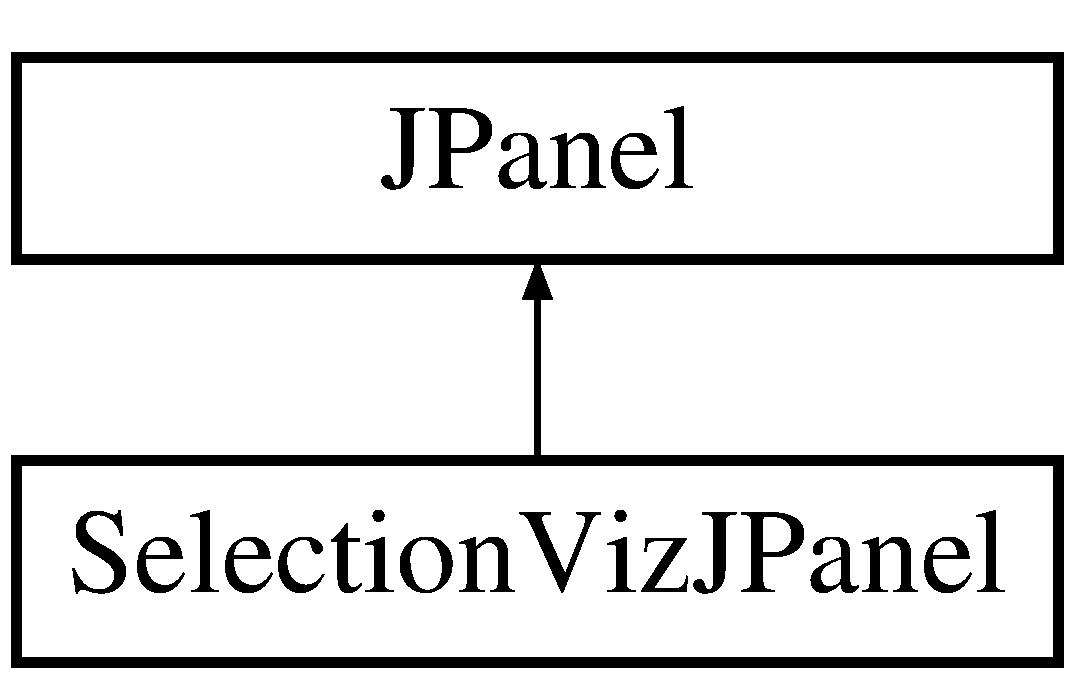
\includegraphics[height=2.000000cm]{class_selection_viz_j_panel}
\end{center}
\end{figure}
\subsection*{Public Member Functions}
\begin{DoxyCompactItemize}
\item 
\hyperlink{class_selection_viz_j_panel_ab3acb1051321159e8cfcc251b6adeb9a}{Selection\-Viz\-J\-Panel} ()
\item 
boolean \hyperlink{class_selection_viz_j_panel_a6287ea60b41d461f06b609340d9c38b4}{Set\-B\-V} (\hyperlink{class_bob_viz}{Bob\-Viz} bv)
\item 
boolean \hyperlink{class_selection_viz_j_panel_ab942f7a1e094e8d3df0df172499c8878}{Set\-Viz\-J\-But\-Enabled} (boolean b)
\item 
boolean \hyperlink{class_selection_viz_j_panel_afe28337fc26eb95b02450f6138977c90}{Set\-Slideshow\-Viz\-J\-But\-Enabled} (boolean b)
\item 
boolean \hyperlink{class_selection_viz_j_panel_ad60f302412430e0e86fe1a6dc9e65d2a}{Get\-Viz\-J\-But\-Enabled} ()
\item 
boolean \hyperlink{class_selection_viz_j_panel_ad585ffba9965244bfe10ce138cc1e3f7}{Get\-Slideshow\-Viz\-J\-But\-Enabled} ()
\item 
boolean \hyperlink{class_selection_viz_j_panel_af9db99d82813968723871bb63985618f}{Set\-Data\-Attribute} ()
\end{DoxyCompactItemize}


\subsection{Detailed Description}
This class passes the data from the G\-U\-I to the constructors of the visualisation types. 

\begin{DoxyDate}{Date}
30/04/2013 
\end{DoxyDate}
\begin{DoxySeeAlso}{See Also}
\hyperlink{_table_8java}{Table.\-java}, \hyperlink{_column_chart_8java}{Column\-Chart.\-java}, Scatter\-Graph.\-java, \hyperlink{_pie_chart_8java}{Pie\-Chart.\-java} 
\end{DoxySeeAlso}


\subsection{Constructor \& Destructor Documentation}
\hypertarget{class_selection_viz_j_panel_ab3acb1051321159e8cfcc251b6adeb9a}{\index{Selection\-Viz\-J\-Panel@{Selection\-Viz\-J\-Panel}!Selection\-Viz\-J\-Panel@{Selection\-Viz\-J\-Panel}}
\index{Selection\-Viz\-J\-Panel@{Selection\-Viz\-J\-Panel}!SelectionVizJPanel@{Selection\-Viz\-J\-Panel}}
\subsubsection[{Selection\-Viz\-J\-Panel}]{\setlength{\rightskip}{0pt plus 5cm}Selection\-Viz\-J\-Panel.\-Selection\-Viz\-J\-Panel (
\begin{DoxyParamCaption}
{}
\end{DoxyParamCaption}
)}}\label{class_selection_viz_j_panel_ab3acb1051321159e8cfcc251b6adeb9a}

\begin{DoxyCode}
25                                 \{
26         
27         \textcolor{comment}{/* create new visualisation button */}
28         m\_VisualizeJBut = \textcolor{keyword}{new} JButton( \textcolor{stringliteral}{"Generate Visualization!"} );
29         \textcolor{comment}{/* create new slideshow visualisation button */}
30         m\_SlideshowVisualizeJBut = \textcolor{keyword}{new} JButton( \textcolor{stringliteral}{"Generate Slideshow!"} );
31 
32         \textcolor{comment}{/* set visualisation font */}
33         m\_VisualizeJBut.setFont( \textcolor{keyword}{new} Font( \textcolor{stringliteral}{"Courier"}, Font.BOLD, FONT\_SIZE ) );
34         m\_VisualizeJBut.setEnabled( \textcolor{keyword}{false} );
35         add( m\_VisualizeJBut );
36         m\_SlideshowVisualizeJBut.setFont( \textcolor{keyword}{new} Font( \textcolor{stringliteral}{"Courier"}, Font.BOLD, FONT\_SIZE ) );
37         m\_SlideshowVisualizeJBut.setEnabled( \textcolor{keyword}{false} );
38         add( m\_SlideshowVisualizeJBut );
39 
40 
41         \textcolor{comment}{/* set listeners */}
42         GenerateVizJPanelEventHandler iJEventHandler = \textcolor{keyword}{new} 
43                 GenerateVizJPanelEventHandler();
44         m\_VisualizeJBut.addActionListener( iJEventHandler );
45         
46         GenerateSlideshowVizJPanelEventHandler iSlideshowJEventHandler = \textcolor{keyword}{new} 
47                 GenerateSlideshowVizJPanelEventHandler();
48         m\_SlideshowVisualizeJBut.addActionListener( iSlideshowJEventHandler );
49         
50     \}
\end{DoxyCode}


\subsection{Member Function Documentation}
\hypertarget{class_selection_viz_j_panel_ad585ffba9965244bfe10ce138cc1e3f7}{\index{Selection\-Viz\-J\-Panel@{Selection\-Viz\-J\-Panel}!Get\-Slideshow\-Viz\-J\-But\-Enabled@{Get\-Slideshow\-Viz\-J\-But\-Enabled}}
\index{Get\-Slideshow\-Viz\-J\-But\-Enabled@{Get\-Slideshow\-Viz\-J\-But\-Enabled}!SelectionVizJPanel@{Selection\-Viz\-J\-Panel}}
\subsubsection[{Get\-Slideshow\-Viz\-J\-But\-Enabled}]{\setlength{\rightskip}{0pt plus 5cm}boolean Selection\-Viz\-J\-Panel.\-Get\-Slideshow\-Viz\-J\-But\-Enabled (
\begin{DoxyParamCaption}
{}
\end{DoxyParamCaption}
)}}\label{class_selection_viz_j_panel_ad585ffba9965244bfe10ce138cc1e3f7}
\begin{DoxyReturn}{Returns}
the state of the slideshow button 
\end{DoxyReturn}

\begin{DoxyCode}
109                                                 \{
110         \textcolor{keywordflow}{return} m\_SlideshowVisualizeJBut.isEnabled();
111     \}
\end{DoxyCode}
\hypertarget{class_selection_viz_j_panel_ad60f302412430e0e86fe1a6dc9e65d2a}{\index{Selection\-Viz\-J\-Panel@{Selection\-Viz\-J\-Panel}!Get\-Viz\-J\-But\-Enabled@{Get\-Viz\-J\-But\-Enabled}}
\index{Get\-Viz\-J\-But\-Enabled@{Get\-Viz\-J\-But\-Enabled}!SelectionVizJPanel@{Selection\-Viz\-J\-Panel}}
\subsubsection[{Get\-Viz\-J\-But\-Enabled}]{\setlength{\rightskip}{0pt plus 5cm}boolean Selection\-Viz\-J\-Panel.\-Get\-Viz\-J\-But\-Enabled (
\begin{DoxyParamCaption}
{}
\end{DoxyParamCaption}
)}}\label{class_selection_viz_j_panel_ad60f302412430e0e86fe1a6dc9e65d2a}
\begin{DoxyReturn}{Returns}
the state of visualise button 
\end{DoxyReturn}

\begin{DoxyCode}
103                                        \{
104         \textcolor{keywordflow}{return} m\_VisualizeJBut.isEnabled();
105     \}
\end{DoxyCode}
\hypertarget{class_selection_viz_j_panel_a6287ea60b41d461f06b609340d9c38b4}{\index{Selection\-Viz\-J\-Panel@{Selection\-Viz\-J\-Panel}!Set\-B\-V@{Set\-B\-V}}
\index{Set\-B\-V@{Set\-B\-V}!SelectionVizJPanel@{Selection\-Viz\-J\-Panel}}
\subsubsection[{Set\-B\-V}]{\setlength{\rightskip}{0pt plus 5cm}boolean Selection\-Viz\-J\-Panel.\-Set\-B\-V (
\begin{DoxyParamCaption}
\item[{{\bf Bob\-Viz}}]{bv}
\end{DoxyParamCaption}
)}}\label{class_selection_viz_j_panel_a6287ea60b41d461f06b609340d9c38b4}
This method will cast the \hyperlink{class_bob_viz}{Bob\-Viz} instance from Bob\-Viz\-Demo. 
\begin{DoxyParams}{Parameters}
{\em bv} & -\/a \hyperlink{class_bob_viz}{Bob\-Viz} object \\
\hline
\end{DoxyParams}
\begin{DoxyReturn}{Returns}
boolean if true 
\end{DoxyReturn}

\begin{DoxyCode}
58                                       \{
59         \textcolor{keywordtype}{boolean} test = \textcolor{keyword}{true};
60         \textcolor{keywordflow}{if}( ( test == \textcolor{keyword}{true} ) && ( bv == null ) ) \{
61             System.err.println( \textcolor{stringliteral}{"GenerateVizJPanel::SetBV() ***Warning, object"}
62                     + \textcolor{stringliteral}{"is null. Value sent: "} + bv );
63         \} \textcolor{keywordflow}{else} \textcolor{keywordflow}{if} ( test == \textcolor{keyword}{true} ) \{
64             System.out.println( \textcolor{stringliteral}{"GenerateVizJPanel::SetBV() Object is valid. "}
65                     + \textcolor{stringliteral}{"Value sent: "} + bv );
66         \}
67         m\_BV = bv;
68         \textcolor{keywordflow}{return} \textcolor{keyword}{true};
69     \}
\end{DoxyCode}
\hypertarget{class_selection_viz_j_panel_af9db99d82813968723871bb63985618f}{\index{Selection\-Viz\-J\-Panel@{Selection\-Viz\-J\-Panel}!Set\-Data\-Attribute@{Set\-Data\-Attribute}}
\index{Set\-Data\-Attribute@{Set\-Data\-Attribute}!SelectionVizJPanel@{Selection\-Viz\-J\-Panel}}
\subsubsection[{Set\-Data\-Attribute}]{\setlength{\rightskip}{0pt plus 5cm}boolean Selection\-Viz\-J\-Panel.\-Set\-Data\-Attribute (
\begin{DoxyParamCaption}
{}
\end{DoxyParamCaption}
)}}\label{class_selection_viz_j_panel_af9db99d82813968723871bb63985618f}
Sets X \& Y axis labels in \hyperlink{class_data_attribute}{Data\-Attribute} \begin{DoxyReturn}{Returns}
boolean true if successful 
\end{DoxyReturn}

\begin{DoxyCode}
117                                       \{
118         m\_BV.\hyperlink{class_bob_viz_acc980a6db181f9ace3279e5dd3fd23b8}{GetDataAttribute}().\hyperlink{class_data_attribute_a434e57b34476663c13eb6dc37ef05cd2}{SetTitle}( m\_BV.
      \hyperlink{class_bob_viz_a10dab616869fe644d16c2ccf78627af5}{GetSettingJPan}().
119                 GetTitle() );
120         m\_BV.\hyperlink{class_bob_viz_acc980a6db181f9ace3279e5dd3fd23b8}{GetDataAttribute}().\hyperlink{class_data_attribute_ab7c3ae470051e011aa22725ad9ebab58}{SetSecondTitle}( m\_BV.
      \hyperlink{class_bob_viz_a10dab616869fe644d16c2ccf78627af5}{GetSettingJPan}().
121                 GetSecondTitle() );
122         \textcolor{comment}{/* store axis label x and y in DataAttribute */}
123         m\_BV.\hyperlink{class_bob_viz_acc980a6db181f9ace3279e5dd3fd23b8}{GetDataAttribute}().\hyperlink{class_data_attribute_a2d8c2f41d2847e3bbcb8b869d15e97f3}{SetAxisLabelX}( m\_BV.
124                 GetSettingJPan().GetAxisLabelX());        
125         m\_BV.\hyperlink{class_bob_viz_acc980a6db181f9ace3279e5dd3fd23b8}{GetDataAttribute}().\hyperlink{class_data_attribute_a31655976e5ce4d6be0b07b0a0bdcf3fc}{SetAxisLabelY}( m\_BV.
126                 GetSettingJPan().GetAxisLabelY());
127         m\_BV.\hyperlink{class_bob_viz_acc980a6db181f9ace3279e5dd3fd23b8}{GetDataAttribute}().\hyperlink{class_data_attribute_a1b57fd911860c75a1aa5ded4c0c2d707}{SetAxisLabelZ}( m\_BV.
128                 GetSettingJPan().GetAxisLabelZ());
129         m\_BV.\hyperlink{class_bob_viz_acc980a6db181f9ace3279e5dd3fd23b8}{GetDataAttribute}().\hyperlink{class_data_attribute_a0749b154967281fc88c3d50b61b82ec7}{SetSecondAxisLabelX}( m\_BV.
130                 GetSettingJPan().GetSecondAxisLabelX());        
131         m\_BV.\hyperlink{class_bob_viz_acc980a6db181f9ace3279e5dd3fd23b8}{GetDataAttribute}().\hyperlink{class_data_attribute_aa991ca454981460ff011efa92a63b83c}{SetSecondAxisLabelY}( m\_BV.
132                 GetSettingJPan().GetSecondAxisLabelY());
133         m\_BV.\hyperlink{class_bob_viz_acc980a6db181f9ace3279e5dd3fd23b8}{GetDataAttribute}().\hyperlink{class_data_attribute_a1b7436f51b0079c492b6451500230329}{SetSecondAxisLabelZ}( m\_BV.
134                 GetSettingJPan().GetSecondAxisLabelZ());
135         
136         m\_BV.\hyperlink{class_bob_viz_acc980a6db181f9ace3279e5dd3fd23b8}{GetDataAttribute}().\hyperlink{class_data_attribute_acd1994e216d21da1f3e7ea2819145fe9}{SetXAxisMin}( m\_BV.
137                 GetSettingJPan().GetXAxisMin());
138         m\_BV.\hyperlink{class_bob_viz_acc980a6db181f9ace3279e5dd3fd23b8}{GetDataAttribute}().\hyperlink{class_data_attribute_a6aedbe05a82f23d6abca00f8b85bf1ff}{SetXAxisMax}( m\_BV.
139                 GetSettingJPan().GetXAxisMax());
140         m\_BV.\hyperlink{class_bob_viz_acc980a6db181f9ace3279e5dd3fd23b8}{GetDataAttribute}().\hyperlink{class_data_attribute_afacd93a87dbe8ed03d4dc9a50e44851f}{SetYAxisMin}( m\_BV.
141                 GetSettingJPan().GetYAxisMin());
142         m\_BV.\hyperlink{class_bob_viz_acc980a6db181f9ace3279e5dd3fd23b8}{GetDataAttribute}().\hyperlink{class_data_attribute_a0098d5256a1b929cf8a84006bb52d1af}{SetYAxisMax}( m\_BV.
143                 GetSettingJPan().GetYAxisMax());
144         
145         m\_BV.\hyperlink{class_bob_viz_acc980a6db181f9ace3279e5dd3fd23b8}{GetDataAttribute}().\hyperlink{class_data_attribute_ad70067aa2addb581e5d654d1cee4cd97}{SetXAxisScale}( m\_BV.
146                 GetSettingJPan().GetXAxisScale());
147         m\_BV.\hyperlink{class_bob_viz_acc980a6db181f9ace3279e5dd3fd23b8}{GetDataAttribute}().\hyperlink{class_data_attribute_a56bf007539747ac6b80c156416336d14}{SetYAxisScale}( m\_BV.
148                 GetSettingJPan().GetYAxisScale());
149         
150         m\_BV.\hyperlink{class_bob_viz_acc980a6db181f9ace3279e5dd3fd23b8}{GetDataAttribute}().\hyperlink{class_data_attribute_ae2965e7960aaf72643f23a1359daf582}{SetChartAuthor}( m\_BV.
151                 GetSettingJPan().GetAuthor());
152         m\_BV.\hyperlink{class_bob_viz_acc980a6db181f9ace3279e5dd3fd23b8}{GetDataAttribute}().\hyperlink{class_data_attribute_abbc4a01ce590f81351c3bb527cf18352}{SetChartDesciption}( m\_BV.
153                 GetSettingJPan().GetDescription());
154         m\_BV.\hyperlink{class_bob_viz_acc980a6db181f9ace3279e5dd3fd23b8}{GetDataAttribute}().\hyperlink{class_data_attribute_aa3848e837d08789f975e82a9753bda5c}{DisplayAll}();
155         
156         m\_BV.\hyperlink{class_bob_viz_acc980a6db181f9ace3279e5dd3fd23b8}{GetDataAttribute}().\hyperlink{class_data_attribute_a46b8473768d9ba3609e5f5994e903a7c}{SetUseDefault}(
157                 m\_BV.\hyperlink{class_bob_viz_a10dab616869fe644d16c2ccf78627af5}{GetSettingJPan}().\hyperlink{class_setting_j_panel_ab9c3cb39831c331a8a8a041655348cc7}{GetDefaultButton}().isSelected());
158         
159         \textcolor{keywordflow}{return} \textcolor{keyword}{true};
160     \}
\end{DoxyCode}
\hypertarget{class_selection_viz_j_panel_afe28337fc26eb95b02450f6138977c90}{\index{Selection\-Viz\-J\-Panel@{Selection\-Viz\-J\-Panel}!Set\-Slideshow\-Viz\-J\-But\-Enabled@{Set\-Slideshow\-Viz\-J\-But\-Enabled}}
\index{Set\-Slideshow\-Viz\-J\-But\-Enabled@{Set\-Slideshow\-Viz\-J\-But\-Enabled}!SelectionVizJPanel@{Selection\-Viz\-J\-Panel}}
\subsubsection[{Set\-Slideshow\-Viz\-J\-But\-Enabled}]{\setlength{\rightskip}{0pt plus 5cm}boolean Selection\-Viz\-J\-Panel.\-Set\-Slideshow\-Viz\-J\-But\-Enabled (
\begin{DoxyParamCaption}
\item[{boolean}]{b}
\end{DoxyParamCaption}
)}}\label{class_selection_viz_j_panel_afe28337fc26eb95b02450f6138977c90}
This method changes the enabled state of the \hyperlink{class_slideshow}{Slideshow} button. 
\begin{DoxyParams}{Parameters}
{\em b} & -\/a boolean object \\
\hline
\end{DoxyParams}
\begin{DoxyReturn}{Returns}
boolean true if successful 
\end{DoxyReturn}

\begin{DoxyCode}
90                                                            \{
91         \textcolor{keywordtype}{boolean} test = \textcolor{keyword}{true};
92         \textcolor{keywordflow}{if} ( test == \textcolor{keyword}{true} ) \{
93             System.out.println( \textcolor{stringliteral}{"GenerateVizJPanel::SetSlideshowVizJButEnabled() m\_"}
94                     + \textcolor{stringliteral}{"SlideshowVisualizeJBut enabled status: "} + b );
95         \}
96         m\_SlideshowVisualizeJBut.setEnabled( b );
97         \textcolor{keywordflow}{return} \textcolor{keyword}{true};
98     \}
\end{DoxyCode}
\hypertarget{class_selection_viz_j_panel_ab942f7a1e094e8d3df0df172499c8878}{\index{Selection\-Viz\-J\-Panel@{Selection\-Viz\-J\-Panel}!Set\-Viz\-J\-But\-Enabled@{Set\-Viz\-J\-But\-Enabled}}
\index{Set\-Viz\-J\-But\-Enabled@{Set\-Viz\-J\-But\-Enabled}!SelectionVizJPanel@{Selection\-Viz\-J\-Panel}}
\subsubsection[{Set\-Viz\-J\-But\-Enabled}]{\setlength{\rightskip}{0pt plus 5cm}boolean Selection\-Viz\-J\-Panel.\-Set\-Viz\-J\-But\-Enabled (
\begin{DoxyParamCaption}
\item[{boolean}]{b}
\end{DoxyParamCaption}
)}}\label{class_selection_viz_j_panel_ab942f7a1e094e8d3df0df172499c8878}
This method changes the enabled state of the visualisation button. 
\begin{DoxyParams}{Parameters}
{\em b} & -\/a boolean object \\
\hline
\end{DoxyParams}
\begin{DoxyReturn}{Returns}
boolean true if successful 
\end{DoxyReturn}

\begin{DoxyCode}
76                                                   \{
77         \textcolor{keywordtype}{boolean} test = \textcolor{keyword}{true};
78         \textcolor{keywordflow}{if} ( test == \textcolor{keyword}{true} ) \{
79             System.out.println( \textcolor{stringliteral}{"GenerateVizJPanel::SetVizJButEnabled() m\_"}
80                     + \textcolor{stringliteral}{"VisualizeJBut enabled status: "} + b );
81         \}
82         m\_VisualizeJBut.setEnabled( b );
83         \textcolor{keywordflow}{return} \textcolor{keyword}{true};
84     \}
\end{DoxyCode}


The documentation for this class was generated from the following file\-:\begin{DoxyCompactItemize}
\item 
\hyperlink{_selection_viz_j_panel_8java}{Selection\-Viz\-J\-Panel.\-java}\end{DoxyCompactItemize}

\hypertarget{class_setting_j_panel}{\section{Setting\-J\-Panel Class Reference}
\label{class_setting_j_panel}\index{Setting\-J\-Panel@{Setting\-J\-Panel}}
}


This class provides the settings for each visualisation.  


Inheritance diagram for Setting\-J\-Panel\-:\begin{figure}[H]
\begin{center}
\leavevmode
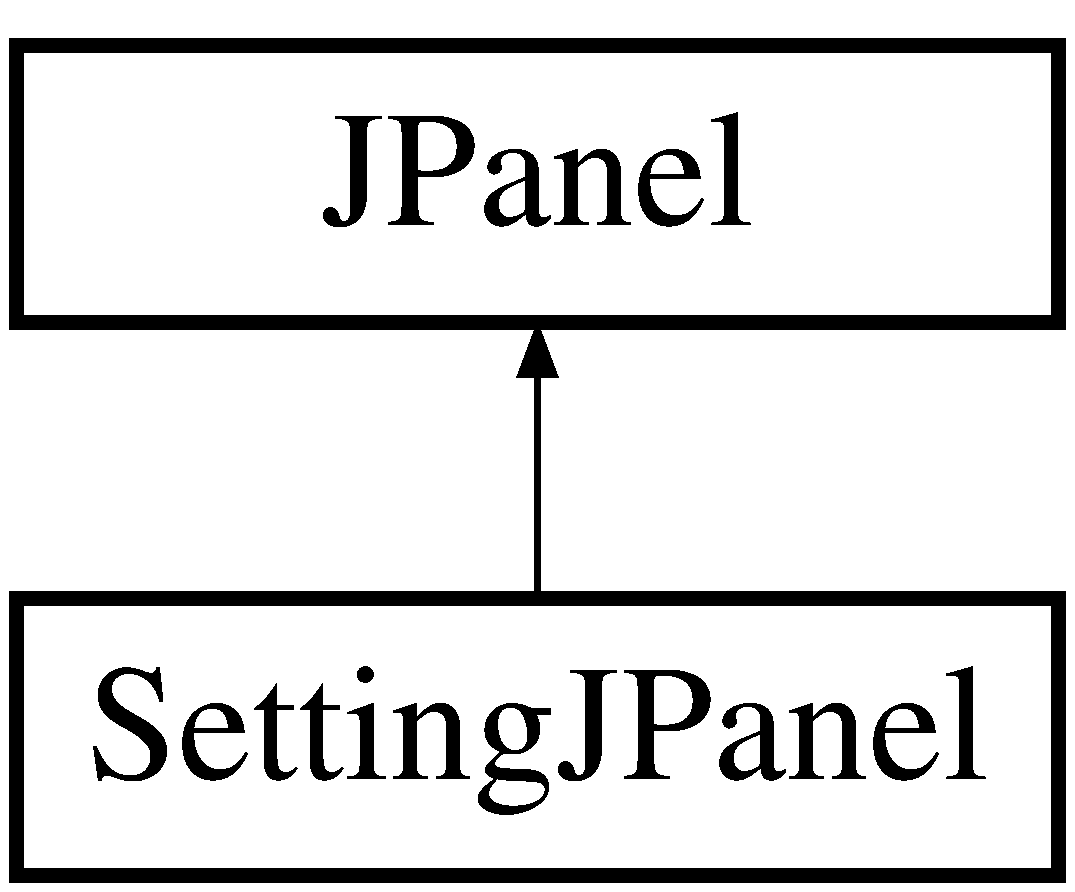
\includegraphics[height=2.000000cm]{class_setting_j_panel}
\end{center}
\end{figure}
\subsection*{Public Member Functions}
\begin{DoxyCompactItemize}
\item 
\hyperlink{class_setting_j_panel_af17c3f4ba101c659fe9eaa7dc6ee7f27}{Setting\-J\-Panel} ()
\item 
double \hyperlink{class_setting_j_panel_a19038ce15f6c0a2a835981e04dd0e3e2}{Get\-X\-Axis\-Min} ()
\item 
double \hyperlink{class_setting_j_panel_ad444ca2c7161cdfb906d1ddeebb5ff23}{Get\-X\-Axis\-Max} ()
\item 
double \hyperlink{class_setting_j_panel_ab7d2ee01bcbb7c2565f987ce4ad7f8a6}{Get\-Y\-Axis\-Min} ()
\item 
double \hyperlink{class_setting_j_panel_abc0018346df79e2c333fceb8100d73ad}{Get\-Y\-Axis\-Max} ()
\item 
double \hyperlink{class_setting_j_panel_af5c40b9861c4f1af69c78beea105ce70}{Get\-X\-Axis\-Scale} ()
\item 
double \hyperlink{class_setting_j_panel_ad8649c6a06816c500e46ac7e2f983de4}{Get\-Y\-Axis\-Scale} ()
\item 
String \hyperlink{class_setting_j_panel_ad77ebfe5f6684e358d613cb3e0daed49}{Get\-Author} ()
\item 
String \hyperlink{class_setting_j_panel_aa830d6ccb04cfe19429b22119a52c127}{Get\-Description} ()
\item 
J\-Toggle\-Button \hyperlink{class_setting_j_panel_ab9c3cb39831c331a8a8a041655348cc7}{Get\-Default\-Button} ()
\item 
J\-Combo\-Box \hyperlink{class_setting_j_panel_ab4d6bc8c6213d9ccaf93509ad43a9a7c}{Get\-Z\-Axis\-Combo\-Box} ()
\item 
J\-Combo\-Box \hyperlink{class_setting_j_panel_af85c5475c2586ace4c6adfaf7c63c708}{Get\-Second\-Z\-Axis\-Combo\-Box} ()
\item 
boolean \hyperlink{class_setting_j_panel_aabfaa9fb1f2cfc91197b0b5cf10e538d}{Set\-B\-V} (\hyperlink{class_bob_viz}{Bob\-Viz} bv)
\item 
boolean \hyperlink{class_setting_j_panel_a0867f721026a690933334532d59fd1c0}{Set\-Settings\-Enabled} (boolean b)
\item 
boolean \hyperlink{class_setting_j_panel_af44d07f356aa8217418fe0878a50f48d}{Set\-Second\-Settings\-Enabled} (boolean b)
\item 
boolean \hyperlink{class_setting_j_panel_afb2b0736bdf6a8a724066b4a7c78a25f}{Set\-Viz\-Sys\-Type} (String\mbox{[}$\,$\mbox{]} headings)
\item 
boolean \hyperlink{class_setting_j_panel_a8c7f693b437db5e8890346d34b68f034}{Set\-Second\-Viz\-Sys\-Type} (String\mbox{[}$\,$\mbox{]} headings)
\item 
String \hyperlink{class_setting_j_panel_a6cfc2b28e65ad6b225137660445e782a}{Get\-Title} ()
\item 
String \hyperlink{class_setting_j_panel_ac3180cd3580d14425b1bdaa66aaf3d98}{Get\-Second\-Title} ()
\item 
String \hyperlink{class_setting_j_panel_a34e7268bb7e2dafb51bff0a81c91ae79}{Get\-Axis\-Label\-X} ()
\item 
String \hyperlink{class_setting_j_panel_a043e52d7819def149ebd16e970aea508}{Get\-Second\-Axis\-Label\-X} ()
\item 
String \hyperlink{class_setting_j_panel_a2e1a90cd3ad567d66ce8a4c99fb59d9e}{Get\-Axis\-Label\-Y} ()
\item 
String \hyperlink{class_setting_j_panel_a6ab00c064d9bc103328188cf01b252c2}{Get\-Second\-Axis\-Label\-Y} ()
\item 
String \hyperlink{class_setting_j_panel_a23ce003414b5fefe6fda97d1c282ccb0}{Get\-Axis\-Label\-Z} ()
\item 
String \hyperlink{class_setting_j_panel_a58e88f0beebb429d7311924a07dae840}{Get\-Second\-Axis\-Label\-Z} ()
\item 
int \hyperlink{class_setting_j_panel_a3f22bf0303fdcd171842558a6577c6ac}{Get\-Selected\-X\-Index} ()
\item 
int \hyperlink{class_setting_j_panel_a08607519a288552eac8b0f4bf89a1a19}{Get\-Second\-Selected\-X\-Index} ()
\item 
int \hyperlink{class_setting_j_panel_a3d94c6447f40c93a1a62a486d9642a9b}{Get\-Selected\-Y\-Index} ()
\item 
int \hyperlink{class_setting_j_panel_a4b52c9cb35b9450fa667942085fbb75f}{Get\-Second\-Selected\-Y\-Index} ()
\item 
int \hyperlink{class_setting_j_panel_a8ca1d551d5ef0db315edca6f123a5e44}{Get\-Selected\-Z\-Index} ()
\item 
int \hyperlink{class_setting_j_panel_a9452c1c3050642bcec0af5591fd9f437}{Get\-Second\-Selected\-Z\-Index} ()
\item 
boolean \hyperlink{class_setting_j_panel_a2ad9d316118129421cd3706f7f4e3998}{Get\-Settings\-Enabled} ()
\item 
boolean \hyperlink{class_setting_j_panel_a64a2366145bd68a57ce6f263b7e0a864}{Get\-Second\-Settings\-Enabled} ()
\item 
int \hyperlink{class_setting_j_panel_a116f4d7091e9f0ed859b7682aa4e1b6b}{Get\-Panel\-Width} ()
\item 
int \hyperlink{class_setting_j_panel_ad1010855cd475f58407a67cdcf210157}{Get\-Panel\-Height} ()
\end{DoxyCompactItemize}
\subsection*{Static Public Member Functions}
\begin{DoxyCompactItemize}
\item 
static void \hyperlink{class_setting_j_panel_a80ff33ccb4055347d74a6de61de63f2a}{main} (String\mbox{[}$\,$\mbox{]} args)
\end{DoxyCompactItemize}


\subsection{Detailed Description}
This class provides the settings for each visualisation. 

\begin{DoxyDate}{Date}
-\/30/04/2013 
\end{DoxyDate}
\begin{DoxySeeAlso}{See Also}
\hyperlink{_bob_viz_8java}{Bob\-Viz.\-java} 
\end{DoxySeeAlso}


\subsection{Constructor \& Destructor Documentation}
\hypertarget{class_setting_j_panel_af17c3f4ba101c659fe9eaa7dc6ee7f27}{\index{Setting\-J\-Panel@{Setting\-J\-Panel}!Setting\-J\-Panel@{Setting\-J\-Panel}}
\index{Setting\-J\-Panel@{Setting\-J\-Panel}!SettingJPanel@{Setting\-J\-Panel}}
\subsubsection[{Setting\-J\-Panel}]{\setlength{\rightskip}{0pt plus 5cm}Setting\-J\-Panel.\-Setting\-J\-Panel (
\begin{DoxyParamCaption}
{}
\end{DoxyParamCaption}
)}}\label{class_setting_j_panel_af17c3f4ba101c659fe9eaa7dc6ee7f27}

\begin{DoxyCode}
30                            \{
31         \textcolor{comment}{/* set new size dimensions */}
32         Dimension size = getPreferredSize();
33         size.width = PAN\_WIDTH;
34         size.height = PAN\_HEIGHT;
35         setPreferredSize( size );
36         
37         setBorder( BorderFactory.createTitledBorder(
38                 BorderFactory.createLineBorder( Color.GRAY ), SELECT\_VIZ\_PREF
39                  ) );
40         setLayout( \textcolor{keyword}{new} FlowLayout( FlowLayout.CENTER ) );
41         
42         \textcolor{comment}{/* create new JPanel */}
43         JPanel centerJPan = \textcolor{keyword}{new} JPanel();
44         centerJPan.setLayout( \textcolor{keyword}{new} GridLayout( GRID\_ROW, GRID\_COL, GRID\_VGAP, 
45                 GRID\_HGAP ) );
46         
47         \textcolor{comment}{/* set default x and y axis */}
48         String[] xAxis = \{\textcolor{stringliteral}{""}\};
49         String[] yAxis = \{\textcolor{stringliteral}{""}\};
50         String[] zAxis = \{\textcolor{stringliteral}{""}\};
51         
52         \textcolor{comment}{/* create new jlabels */}
53         JLabel blank = \textcolor{keyword}{new} JLabel( \textcolor{stringliteral}{""} );
54         JLabel firstCSVTitle = \textcolor{keyword}{new} JLabel( \textcolor{stringliteral}{"First CSV"} );
55         JLabel secondCSVTitle = \textcolor{keyword}{new} JLabel( \textcolor{stringliteral}{"Second CSV"} );
56         JLabel chartTitJLab = \textcolor{keyword}{new} JLabel( \textcolor{stringliteral}{"Chart title:"} );
57         JLabel xAxisJLab = \textcolor{keyword}{new} JLabel( \textcolor{stringliteral}{"X axis:"} );
58         JLabel yAxisJLab = \textcolor{keyword}{new} JLabel( \textcolor{stringliteral}{"Y axis:"} );
59         JLabel zAxisJLab = \textcolor{keyword}{new} JLabel( \textcolor{stringliteral}{"Z axis:"} );
60         
61         \textcolor{comment}{/* create new input fields */}
62         m\_ChartTitJTextF = \textcolor{keyword}{new} JTextField( TEXT\_FIELD\_LEN );
63         m\_xAxisJCom = \textcolor{keyword}{new} JComboBox( xAxis );
64         m\_yAxisJCom = \textcolor{keyword}{new} JComboBox( yAxis );
65         m\_zAxisJCom = \textcolor{keyword}{new} JComboBox( zAxis );
66         m\_zAxisJCom.setEnabled(\textcolor{keyword}{false});
67         
68         m\_SecondChartTitJTextF = \textcolor{keyword}{new} JTextField( TEXT\_FIELD\_LEN );
69         m\_SecondxAxisJCom = \textcolor{keyword}{new} JComboBox( xAxis );
70         m\_SecondyAxisJCom = \textcolor{keyword}{new} JComboBox( yAxis );
71         m\_SecondzAxisJCom = \textcolor{keyword}{new} JComboBox( zAxis );
72         m\_SecondzAxisJCom.setEnabled(\textcolor{keyword}{false});
73         
74         
75         \textcolor{comment}{/* set all input fields disabled by default */}
76         m\_ChartTitJTextF.setEnabled( \textcolor{keyword}{false} );
77         m\_SecondChartTitJTextF.setEnabled( \textcolor{keyword}{false} );
78         m\_xAxisJCom.setEnabled( \textcolor{keyword}{false} );
79         m\_yAxisJCom.setEnabled( \textcolor{keyword}{false} );
80         m\_zAxisJCom.setEnabled( \textcolor{keyword}{false} );
81         m\_SecondxAxisJCom.setEnabled( \textcolor{keyword}{false} );
82         m\_SecondyAxisJCom.setEnabled( \textcolor{keyword}{false} );
83         m\_SecondzAxisJCom.setEnabled( \textcolor{keyword}{false} );
84         m\_AdvancedButton.setEnabled( \textcolor{keyword}{false} );
85         
86         \textcolor{comment}{/* add all components to centerJPan */}
87         centerJPan.add( blank );
88         centerJPan.add( firstCSVTitle );
89         centerJPan.add( secondCSVTitle );
90         centerJPan.add( chartTitJLab );
91         centerJPan.add( m\_ChartTitJTextF );
92         centerJPan.add( m\_SecondChartTitJTextF );
93         centerJPan.add( xAxisJLab );
94         centerJPan.add( m\_xAxisJCom );
95         centerJPan.add( m\_SecondxAxisJCom );
96         centerJPan.add( yAxisJLab );
97         centerJPan.add( m\_yAxisJCom );
98         centerJPan.add( m\_SecondyAxisJCom );
99         centerJPan.add( zAxisJLab );
100         centerJPan.add( m\_zAxisJCom );
101         centerJPan.add( m\_SecondzAxisJCom );
102         centerJPan.add( m\_AdvancedButton );
103         
104         \textcolor{comment}{/* add centerJPan to SettingJPanel */}
105         add( centerJPan );
106         
107         \textcolor{comment}{/* set listeners */}
108         SettingJPanelEventHandler iJEventHandler = \textcolor{keyword}{new} 
109                 SettingJPanelEventHandler();
110         m\_xAxisJCom.addActionListener( iJEventHandler );
111         m\_yAxisJCom.addActionListener( iJEventHandler );
112         m\_zAxisJCom.addActionListener( iJEventHandler );
113         
114         m\_AdvancedButton.addActionListener( iJEventHandler ); 
115         
116         SettingSecondJPanelEventHandler iSecondJEventHandler = \textcolor{keyword}{new} 
117                 SettingSecondJPanelEventHandler();
118         m\_SecondxAxisJCom.addActionListener( iSecondJEventHandler );
119         m\_SecondyAxisJCom.addActionListener( iSecondJEventHandler );
120         m\_SecondzAxisJCom.addActionListener( iSecondJEventHandler );
121         
122     \}
\end{DoxyCode}


\subsection{Member Function Documentation}
\hypertarget{class_setting_j_panel_ad77ebfe5f6684e358d613cb3e0daed49}{\index{Setting\-J\-Panel@{Setting\-J\-Panel}!Get\-Author@{Get\-Author}}
\index{Get\-Author@{Get\-Author}!SettingJPanel@{Setting\-J\-Panel}}
\subsubsection[{Get\-Author}]{\setlength{\rightskip}{0pt plus 5cm}String Setting\-J\-Panel.\-Get\-Author (
\begin{DoxyParamCaption}
{}
\end{DoxyParamCaption}
)}}\label{class_setting_j_panel_ad77ebfe5f6684e358d613cb3e0daed49}
Gets Authour Text

\begin{DoxyReturn}{Returns}
Author Field 
\end{DoxyReturn}

\begin{DoxyCode}
176                               \{
177         \textcolor{keywordflow}{return} m\_SettingPanel.\hyperlink{class_more_setting_j_panel_a3940f844aa7de03b4607a3ce010eaa1f}{GetAuthor}();
178     \}
\end{DoxyCode}
\hypertarget{class_setting_j_panel_a34e7268bb7e2dafb51bff0a81c91ae79}{\index{Setting\-J\-Panel@{Setting\-J\-Panel}!Get\-Axis\-Label\-X@{Get\-Axis\-Label\-X}}
\index{Get\-Axis\-Label\-X@{Get\-Axis\-Label\-X}!SettingJPanel@{Setting\-J\-Panel}}
\subsubsection[{Get\-Axis\-Label\-X}]{\setlength{\rightskip}{0pt plus 5cm}String Setting\-J\-Panel.\-Get\-Axis\-Label\-X (
\begin{DoxyParamCaption}
{}
\end{DoxyParamCaption}
)}}\label{class_setting_j_panel_a34e7268bb7e2dafb51bff0a81c91ae79}
This method will return the x axis label. \begin{DoxyReturn}{Returns}
String -\/ the current x axis label. 
\end{DoxyReturn}

\begin{DoxyCode}
314                                   \{
315         \textcolor{keywordflow}{return} (String) m\_xAxisJCom.getSelectedItem();
316     \}
\end{DoxyCode}
\hypertarget{class_setting_j_panel_a2e1a90cd3ad567d66ce8a4c99fb59d9e}{\index{Setting\-J\-Panel@{Setting\-J\-Panel}!Get\-Axis\-Label\-Y@{Get\-Axis\-Label\-Y}}
\index{Get\-Axis\-Label\-Y@{Get\-Axis\-Label\-Y}!SettingJPanel@{Setting\-J\-Panel}}
\subsubsection[{Get\-Axis\-Label\-Y}]{\setlength{\rightskip}{0pt plus 5cm}String Setting\-J\-Panel.\-Get\-Axis\-Label\-Y (
\begin{DoxyParamCaption}
{}
\end{DoxyParamCaption}
)}}\label{class_setting_j_panel_a2e1a90cd3ad567d66ce8a4c99fb59d9e}
This method will return the y axis label. \begin{DoxyReturn}{Returns}
String -\/ the current y axis label. 
\end{DoxyReturn}

\begin{DoxyCode}
329                                   \{
330         \textcolor{keywordflow}{return} (String) m\_yAxisJCom.getSelectedItem();
331     \}
\end{DoxyCode}
\hypertarget{class_setting_j_panel_a23ce003414b5fefe6fda97d1c282ccb0}{\index{Setting\-J\-Panel@{Setting\-J\-Panel}!Get\-Axis\-Label\-Z@{Get\-Axis\-Label\-Z}}
\index{Get\-Axis\-Label\-Z@{Get\-Axis\-Label\-Z}!SettingJPanel@{Setting\-J\-Panel}}
\subsubsection[{Get\-Axis\-Label\-Z}]{\setlength{\rightskip}{0pt plus 5cm}String Setting\-J\-Panel.\-Get\-Axis\-Label\-Z (
\begin{DoxyParamCaption}
{}
\end{DoxyParamCaption}
)}}\label{class_setting_j_panel_a23ce003414b5fefe6fda97d1c282ccb0}
This method will return the z axis label. \begin{DoxyReturn}{Returns}
String -\/ the current z axis label. 
\end{DoxyReturn}

\begin{DoxyCode}
344                                    \{
345          \textcolor{keywordflow}{return} (String) m\_zAxisJCom.getSelectedItem();
346      \}
\end{DoxyCode}
\hypertarget{class_setting_j_panel_ab9c3cb39831c331a8a8a041655348cc7}{\index{Setting\-J\-Panel@{Setting\-J\-Panel}!Get\-Default\-Button@{Get\-Default\-Button}}
\index{Get\-Default\-Button@{Get\-Default\-Button}!SettingJPanel@{Setting\-J\-Panel}}
\subsubsection[{Get\-Default\-Button}]{\setlength{\rightskip}{0pt plus 5cm}J\-Toggle\-Button Setting\-J\-Panel.\-Get\-Default\-Button (
\begin{DoxyParamCaption}
{}
\end{DoxyParamCaption}
)}}\label{class_setting_j_panel_ab9c3cb39831c331a8a8a041655348cc7}
Gets Default Button

\begin{DoxyReturn}{Returns}
Default Button 
\end{DoxyReturn}

\begin{DoxyCode}
192                                             \{
193         \textcolor{keywordflow}{return} m\_SettingPanel.\hyperlink{class_more_setting_j_panel_ab1f181103d7e162919eb257a3b0d04ca}{GetDefaultButton}();
194     \}
\end{DoxyCode}
\hypertarget{class_setting_j_panel_aa830d6ccb04cfe19429b22119a52c127}{\index{Setting\-J\-Panel@{Setting\-J\-Panel}!Get\-Description@{Get\-Description}}
\index{Get\-Description@{Get\-Description}!SettingJPanel@{Setting\-J\-Panel}}
\subsubsection[{Get\-Description}]{\setlength{\rightskip}{0pt plus 5cm}String Setting\-J\-Panel.\-Get\-Description (
\begin{DoxyParamCaption}
{}
\end{DoxyParamCaption}
)}}\label{class_setting_j_panel_aa830d6ccb04cfe19429b22119a52c127}
Gets Description Text

\begin{DoxyReturn}{Returns}
Description Text Field 
\end{DoxyReturn}

\begin{DoxyCode}
184                                    \{
185         \textcolor{keywordflow}{return} m\_SettingPanel.\hyperlink{class_more_setting_j_panel_a02e5419e3a676912f28da9c6bbebc464}{GetDescription}();
186     \}
\end{DoxyCode}
\hypertarget{class_setting_j_panel_ad1010855cd475f58407a67cdcf210157}{\index{Setting\-J\-Panel@{Setting\-J\-Panel}!Get\-Panel\-Height@{Get\-Panel\-Height}}
\index{Get\-Panel\-Height@{Get\-Panel\-Height}!SettingJPanel@{Setting\-J\-Panel}}
\subsubsection[{Get\-Panel\-Height}]{\setlength{\rightskip}{0pt plus 5cm}int Setting\-J\-Panel.\-Get\-Panel\-Height (
\begin{DoxyParamCaption}
{}
\end{DoxyParamCaption}
)}}\label{class_setting_j_panel_ad1010855cd475f58407a67cdcf210157}
Gets Panel Height

\begin{DoxyReturn}{Returns}
Panel Height 
\end{DoxyReturn}

\begin{DoxyCode}
434                                 \{
435         \textcolor{keywordflow}{return} PAN\_HEIGHT;
436     \}
\end{DoxyCode}
\hypertarget{class_setting_j_panel_a116f4d7091e9f0ed859b7682aa4e1b6b}{\index{Setting\-J\-Panel@{Setting\-J\-Panel}!Get\-Panel\-Width@{Get\-Panel\-Width}}
\index{Get\-Panel\-Width@{Get\-Panel\-Width}!SettingJPanel@{Setting\-J\-Panel}}
\subsubsection[{Get\-Panel\-Width}]{\setlength{\rightskip}{0pt plus 5cm}int Setting\-J\-Panel.\-Get\-Panel\-Width (
\begin{DoxyParamCaption}
{}
\end{DoxyParamCaption}
)}}\label{class_setting_j_panel_a116f4d7091e9f0ed859b7682aa4e1b6b}
Gets Panel Width

\begin{DoxyReturn}{Returns}
Panel Width 
\end{DoxyReturn}

\begin{DoxyCode}
426                                \{
427         \textcolor{keywordflow}{return} PAN\_WIDTH;
428     \}
\end{DoxyCode}
\hypertarget{class_setting_j_panel_a043e52d7819def149ebd16e970aea508}{\index{Setting\-J\-Panel@{Setting\-J\-Panel}!Get\-Second\-Axis\-Label\-X@{Get\-Second\-Axis\-Label\-X}}
\index{Get\-Second\-Axis\-Label\-X@{Get\-Second\-Axis\-Label\-X}!SettingJPanel@{Setting\-J\-Panel}}
\subsubsection[{Get\-Second\-Axis\-Label\-X}]{\setlength{\rightskip}{0pt plus 5cm}String Setting\-J\-Panel.\-Get\-Second\-Axis\-Label\-X (
\begin{DoxyParamCaption}
{}
\end{DoxyParamCaption}
)}}\label{class_setting_j_panel_a043e52d7819def149ebd16e970aea508}
This method will return the second x axis label. \begin{DoxyReturn}{Returns}
String -\/ the current x axis label. 
\end{DoxyReturn}

\begin{DoxyCode}
321                                         \{
322         \textcolor{keywordflow}{return} (String) m\_SecondxAxisJCom.getSelectedItem();
323     \}
\end{DoxyCode}
\hypertarget{class_setting_j_panel_a6ab00c064d9bc103328188cf01b252c2}{\index{Setting\-J\-Panel@{Setting\-J\-Panel}!Get\-Second\-Axis\-Label\-Y@{Get\-Second\-Axis\-Label\-Y}}
\index{Get\-Second\-Axis\-Label\-Y@{Get\-Second\-Axis\-Label\-Y}!SettingJPanel@{Setting\-J\-Panel}}
\subsubsection[{Get\-Second\-Axis\-Label\-Y}]{\setlength{\rightskip}{0pt plus 5cm}String Setting\-J\-Panel.\-Get\-Second\-Axis\-Label\-Y (
\begin{DoxyParamCaption}
{}
\end{DoxyParamCaption}
)}}\label{class_setting_j_panel_a6ab00c064d9bc103328188cf01b252c2}
This method will return the second y axis label. \begin{DoxyReturn}{Returns}
String -\/ the current y axis label. 
\end{DoxyReturn}

\begin{DoxyCode}
336                                         \{
337         \textcolor{keywordflow}{return} (String) m\_SecondyAxisJCom.getSelectedItem();
338     \}
\end{DoxyCode}
\hypertarget{class_setting_j_panel_a58e88f0beebb429d7311924a07dae840}{\index{Setting\-J\-Panel@{Setting\-J\-Panel}!Get\-Second\-Axis\-Label\-Z@{Get\-Second\-Axis\-Label\-Z}}
\index{Get\-Second\-Axis\-Label\-Z@{Get\-Second\-Axis\-Label\-Z}!SettingJPanel@{Setting\-J\-Panel}}
\subsubsection[{Get\-Second\-Axis\-Label\-Z}]{\setlength{\rightskip}{0pt plus 5cm}String Setting\-J\-Panel.\-Get\-Second\-Axis\-Label\-Z (
\begin{DoxyParamCaption}
{}
\end{DoxyParamCaption}
)}}\label{class_setting_j_panel_a58e88f0beebb429d7311924a07dae840}
This method will return the second z axis label. \begin{DoxyReturn}{Returns}
String -\/ the current z axis label. 
\end{DoxyReturn}

\begin{DoxyCode}
351                                          \{
352          \textcolor{keywordflow}{return} (String) m\_SecondzAxisJCom.getSelectedItem();
353      \}
\end{DoxyCode}
\hypertarget{class_setting_j_panel_a08607519a288552eac8b0f4bf89a1a19}{\index{Setting\-J\-Panel@{Setting\-J\-Panel}!Get\-Second\-Selected\-X\-Index@{Get\-Second\-Selected\-X\-Index}}
\index{Get\-Second\-Selected\-X\-Index@{Get\-Second\-Selected\-X\-Index}!SettingJPanel@{Setting\-J\-Panel}}
\subsubsection[{Get\-Second\-Selected\-X\-Index}]{\setlength{\rightskip}{0pt plus 5cm}int Setting\-J\-Panel.\-Get\-Second\-Selected\-X\-Index (
\begin{DoxyParamCaption}
{}
\end{DoxyParamCaption}
)}}\label{class_setting_j_panel_a08607519a288552eac8b0f4bf89a1a19}
This method will return the current second x index. \begin{DoxyReturn}{Returns}
int -\/ the current selected x index. 
\end{DoxyReturn}

\begin{DoxyCode}
366                                          \{
367         \textcolor{keywordflow}{return} m\_SecondxAxisJCom.getSelectedIndex();
368     \}
\end{DoxyCode}
\hypertarget{class_setting_j_panel_a4b52c9cb35b9450fa667942085fbb75f}{\index{Setting\-J\-Panel@{Setting\-J\-Panel}!Get\-Second\-Selected\-Y\-Index@{Get\-Second\-Selected\-Y\-Index}}
\index{Get\-Second\-Selected\-Y\-Index@{Get\-Second\-Selected\-Y\-Index}!SettingJPanel@{Setting\-J\-Panel}}
\subsubsection[{Get\-Second\-Selected\-Y\-Index}]{\setlength{\rightskip}{0pt plus 5cm}int Setting\-J\-Panel.\-Get\-Second\-Selected\-Y\-Index (
\begin{DoxyParamCaption}
{}
\end{DoxyParamCaption}
)}}\label{class_setting_j_panel_a4b52c9cb35b9450fa667942085fbb75f}
This method will return the current second y index. \begin{DoxyReturn}{Returns}
int -\/ the current selected y index. 
\end{DoxyReturn}

\begin{DoxyCode}
381                                          \{
382         \textcolor{keywordflow}{return} m\_SecondyAxisJCom.getSelectedIndex();
383     \}
\end{DoxyCode}
\hypertarget{class_setting_j_panel_a9452c1c3050642bcec0af5591fd9f437}{\index{Setting\-J\-Panel@{Setting\-J\-Panel}!Get\-Second\-Selected\-Z\-Index@{Get\-Second\-Selected\-Z\-Index}}
\index{Get\-Second\-Selected\-Z\-Index@{Get\-Second\-Selected\-Z\-Index}!SettingJPanel@{Setting\-J\-Panel}}
\subsubsection[{Get\-Second\-Selected\-Z\-Index}]{\setlength{\rightskip}{0pt plus 5cm}int Setting\-J\-Panel.\-Get\-Second\-Selected\-Z\-Index (
\begin{DoxyParamCaption}
{}
\end{DoxyParamCaption}
)}}\label{class_setting_j_panel_a9452c1c3050642bcec0af5591fd9f437}
This method will return the current second z index. \begin{DoxyReturn}{Returns}
int -\/ the current selected z index. 
\end{DoxyReturn}

\begin{DoxyCode}
396                                           \{
397          \textcolor{keywordflow}{return} m\_SecondzAxisJCom.getSelectedIndex();
398      \}
\end{DoxyCode}
\hypertarget{class_setting_j_panel_a64a2366145bd68a57ce6f263b7e0a864}{\index{Setting\-J\-Panel@{Setting\-J\-Panel}!Get\-Second\-Settings\-Enabled@{Get\-Second\-Settings\-Enabled}}
\index{Get\-Second\-Settings\-Enabled@{Get\-Second\-Settings\-Enabled}!SettingJPanel@{Setting\-J\-Panel}}
\subsubsection[{Get\-Second\-Settings\-Enabled}]{\setlength{\rightskip}{0pt plus 5cm}boolean Setting\-J\-Panel.\-Get\-Second\-Settings\-Enabled (
\begin{DoxyParamCaption}
{}
\end{DoxyParamCaption}
)}}\label{class_setting_j_panel_a64a2366145bd68a57ce6f263b7e0a864}
This method will check if all second\-Settings are enabled. \begin{DoxyReturn}{Returns}
boolean -\/ the result of all second\-Setting objects (to check if they're enabled). 
\end{DoxyReturn}

\begin{DoxyCode}
415                                               \{
416         \textcolor{keywordflow}{return} m\_SecondChartTitJTextF.isEnabled()
417                 && m\_SecondxAxisJCom.isEnabled()
418                 && m\_SecondyAxisJCom.isEnabled()
419                 && m\_AdvancedButton.isEnabled();
420     \}
\end{DoxyCode}
\hypertarget{class_setting_j_panel_ac3180cd3580d14425b1bdaa66aaf3d98}{\index{Setting\-J\-Panel@{Setting\-J\-Panel}!Get\-Second\-Title@{Get\-Second\-Title}}
\index{Get\-Second\-Title@{Get\-Second\-Title}!SettingJPanel@{Setting\-J\-Panel}}
\subsubsection[{Get\-Second\-Title}]{\setlength{\rightskip}{0pt plus 5cm}String Setting\-J\-Panel.\-Get\-Second\-Title (
\begin{DoxyParamCaption}
{}
\end{DoxyParamCaption}
)}}\label{class_setting_j_panel_ac3180cd3580d14425b1bdaa66aaf3d98}
This method will return the second title of the visualisation. \begin{DoxyReturn}{Returns}
String -\/ the current title. 
\end{DoxyReturn}

\begin{DoxyCode}
305                                    \{
306         m\_SecondTitle = m\_SecondChartTitJTextF.getText();
307         \textcolor{keywordflow}{return} m\_SecondTitle;
308     \}
\end{DoxyCode}
\hypertarget{class_setting_j_panel_af85c5475c2586ace4c6adfaf7c63c708}{\index{Setting\-J\-Panel@{Setting\-J\-Panel}!Get\-Second\-Z\-Axis\-Combo\-Box@{Get\-Second\-Z\-Axis\-Combo\-Box}}
\index{Get\-Second\-Z\-Axis\-Combo\-Box@{Get\-Second\-Z\-Axis\-Combo\-Box}!SettingJPanel@{Setting\-J\-Panel}}
\subsubsection[{Get\-Second\-Z\-Axis\-Combo\-Box}]{\setlength{\rightskip}{0pt plus 5cm}J\-Combo\-Box Setting\-J\-Panel.\-Get\-Second\-Z\-Axis\-Combo\-Box (
\begin{DoxyParamCaption}
{}
\end{DoxyParamCaption}
)}}\label{class_setting_j_panel_af85c5475c2586ace4c6adfaf7c63c708}
Gets Second Z\-Axis Combo Box

\begin{DoxyReturn}{Returns}
Second\-J\-Combo\-Box Z\-Axis value 
\end{DoxyReturn}

\begin{DoxyCode}
208                                               \{
209         \textcolor{keywordflow}{return} m\_SecondzAxisJCom;
210     \}
\end{DoxyCode}
\hypertarget{class_setting_j_panel_a3f22bf0303fdcd171842558a6577c6ac}{\index{Setting\-J\-Panel@{Setting\-J\-Panel}!Get\-Selected\-X\-Index@{Get\-Selected\-X\-Index}}
\index{Get\-Selected\-X\-Index@{Get\-Selected\-X\-Index}!SettingJPanel@{Setting\-J\-Panel}}
\subsubsection[{Get\-Selected\-X\-Index}]{\setlength{\rightskip}{0pt plus 5cm}int Setting\-J\-Panel.\-Get\-Selected\-X\-Index (
\begin{DoxyParamCaption}
{}
\end{DoxyParamCaption}
)}}\label{class_setting_j_panel_a3f22bf0303fdcd171842558a6577c6ac}
This method will return the current x index. \begin{DoxyReturn}{Returns}
int -\/ the current selected x index. 
\end{DoxyReturn}

\begin{DoxyCode}
359                                    \{
360         \textcolor{keywordflow}{return} m\_xAxisJCom.getSelectedIndex();
361     \}
\end{DoxyCode}
\hypertarget{class_setting_j_panel_a3d94c6447f40c93a1a62a486d9642a9b}{\index{Setting\-J\-Panel@{Setting\-J\-Panel}!Get\-Selected\-Y\-Index@{Get\-Selected\-Y\-Index}}
\index{Get\-Selected\-Y\-Index@{Get\-Selected\-Y\-Index}!SettingJPanel@{Setting\-J\-Panel}}
\subsubsection[{Get\-Selected\-Y\-Index}]{\setlength{\rightskip}{0pt plus 5cm}int Setting\-J\-Panel.\-Get\-Selected\-Y\-Index (
\begin{DoxyParamCaption}
{}
\end{DoxyParamCaption}
)}}\label{class_setting_j_panel_a3d94c6447f40c93a1a62a486d9642a9b}
This method will return the current y index. \begin{DoxyReturn}{Returns}
int -\/ the current selected y index. 
\end{DoxyReturn}

\begin{DoxyCode}
374                                    \{
375         \textcolor{keywordflow}{return} m\_yAxisJCom.getSelectedIndex();
376     \}
\end{DoxyCode}
\hypertarget{class_setting_j_panel_a8ca1d551d5ef0db315edca6f123a5e44}{\index{Setting\-J\-Panel@{Setting\-J\-Panel}!Get\-Selected\-Z\-Index@{Get\-Selected\-Z\-Index}}
\index{Get\-Selected\-Z\-Index@{Get\-Selected\-Z\-Index}!SettingJPanel@{Setting\-J\-Panel}}
\subsubsection[{Get\-Selected\-Z\-Index}]{\setlength{\rightskip}{0pt plus 5cm}int Setting\-J\-Panel.\-Get\-Selected\-Z\-Index (
\begin{DoxyParamCaption}
{}
\end{DoxyParamCaption}
)}}\label{class_setting_j_panel_a8ca1d551d5ef0db315edca6f123a5e44}
This method will return the current z index. \begin{DoxyReturn}{Returns}
int -\/ the current selected z index. 
\end{DoxyReturn}

\begin{DoxyCode}
389                                     \{
390          \textcolor{keywordflow}{return} m\_zAxisJCom.getSelectedIndex();
391      \}
\end{DoxyCode}
\hypertarget{class_setting_j_panel_a2ad9d316118129421cd3706f7f4e3998}{\index{Setting\-J\-Panel@{Setting\-J\-Panel}!Get\-Settings\-Enabled@{Get\-Settings\-Enabled}}
\index{Get\-Settings\-Enabled@{Get\-Settings\-Enabled}!SettingJPanel@{Setting\-J\-Panel}}
\subsubsection[{Get\-Settings\-Enabled}]{\setlength{\rightskip}{0pt plus 5cm}boolean Setting\-J\-Panel.\-Get\-Settings\-Enabled (
\begin{DoxyParamCaption}
{}
\end{DoxyParamCaption}
)}}\label{class_setting_j_panel_a2ad9d316118129421cd3706f7f4e3998}
This method will check if all settings are enabled. \begin{DoxyReturn}{Returns}
boolean -\/ the result of all setting objects (to check if they're enabled). 
\end{DoxyReturn}

\begin{DoxyCode}
404                                         \{
405        \textcolor{keywordflow}{return} m\_ChartTitJTextF.isEnabled()
406                && m\_xAxisJCom.isEnabled()
407                && m\_yAxisJCom.isEnabled()
408                && m\_AdvancedButton.isEnabled();
409    \}
\end{DoxyCode}
\hypertarget{class_setting_j_panel_a6cfc2b28e65ad6b225137660445e782a}{\index{Setting\-J\-Panel@{Setting\-J\-Panel}!Get\-Title@{Get\-Title}}
\index{Get\-Title@{Get\-Title}!SettingJPanel@{Setting\-J\-Panel}}
\subsubsection[{Get\-Title}]{\setlength{\rightskip}{0pt plus 5cm}String Setting\-J\-Panel.\-Get\-Title (
\begin{DoxyParamCaption}
{}
\end{DoxyParamCaption}
)}}\label{class_setting_j_panel_a6cfc2b28e65ad6b225137660445e782a}
This method will return the title of the visualisation. \begin{DoxyReturn}{Returns}
String -\/ the current title. 
\end{DoxyReturn}

\begin{DoxyCode}
297                              \{
298         m\_Title = m\_ChartTitJTextF.getText();
299         \textcolor{keywordflow}{return} m\_Title;
300     \}
\end{DoxyCode}
\hypertarget{class_setting_j_panel_ad444ca2c7161cdfb906d1ddeebb5ff23}{\index{Setting\-J\-Panel@{Setting\-J\-Panel}!Get\-X\-Axis\-Max@{Get\-X\-Axis\-Max}}
\index{Get\-X\-Axis\-Max@{Get\-X\-Axis\-Max}!SettingJPanel@{Setting\-J\-Panel}}
\subsubsection[{Get\-X\-Axis\-Max}]{\setlength{\rightskip}{0pt plus 5cm}double Setting\-J\-Panel.\-Get\-X\-Axis\-Max (
\begin{DoxyParamCaption}
{}
\end{DoxyParamCaption}
)}}\label{class_setting_j_panel_ad444ca2c7161cdfb906d1ddeebb5ff23}
Gets X Axis Max Field

\begin{DoxyReturn}{Returns}
X Axis Max Field 
\end{DoxyReturn}

\begin{DoxyCode}
136                                 \{
137         \textcolor{keywordflow}{return} m\_SettingPanel.\hyperlink{class_more_setting_j_panel_a2de92046bd03e4d6173acf6528439f53}{GetXAxisMax}();
138     \}
\end{DoxyCode}
\hypertarget{class_setting_j_panel_a19038ce15f6c0a2a835981e04dd0e3e2}{\index{Setting\-J\-Panel@{Setting\-J\-Panel}!Get\-X\-Axis\-Min@{Get\-X\-Axis\-Min}}
\index{Get\-X\-Axis\-Min@{Get\-X\-Axis\-Min}!SettingJPanel@{Setting\-J\-Panel}}
\subsubsection[{Get\-X\-Axis\-Min}]{\setlength{\rightskip}{0pt plus 5cm}double Setting\-J\-Panel.\-Get\-X\-Axis\-Min (
\begin{DoxyParamCaption}
{}
\end{DoxyParamCaption}
)}}\label{class_setting_j_panel_a19038ce15f6c0a2a835981e04dd0e3e2}
Gets X Axis Min Field

\begin{DoxyReturn}{Returns}
X Axis Min Field 
\end{DoxyReturn}

\begin{DoxyCode}
128                                 \{
129         \textcolor{keywordflow}{return} m\_SettingPanel.\hyperlink{class_more_setting_j_panel_a497d4195007c03bfd6dbf909904f001d}{GetXAxisMin}();
130     \}
\end{DoxyCode}
\hypertarget{class_setting_j_panel_af5c40b9861c4f1af69c78beea105ce70}{\index{Setting\-J\-Panel@{Setting\-J\-Panel}!Get\-X\-Axis\-Scale@{Get\-X\-Axis\-Scale}}
\index{Get\-X\-Axis\-Scale@{Get\-X\-Axis\-Scale}!SettingJPanel@{Setting\-J\-Panel}}
\subsubsection[{Get\-X\-Axis\-Scale}]{\setlength{\rightskip}{0pt plus 5cm}double Setting\-J\-Panel.\-Get\-X\-Axis\-Scale (
\begin{DoxyParamCaption}
{}
\end{DoxyParamCaption}
)}}\label{class_setting_j_panel_af5c40b9861c4f1af69c78beea105ce70}
Gets X Axis Scale Field

\begin{DoxyReturn}{Returns}
X Axis Scale Field 
\end{DoxyReturn}

\begin{DoxyCode}
160                                   \{
161         \textcolor{keywordflow}{return} m\_SettingPanel.\hyperlink{class_more_setting_j_panel_afb3b2d456021f75e7d5ca438da32c5ad}{GetXAxisScale}();
162     \}
\end{DoxyCode}
\hypertarget{class_setting_j_panel_abc0018346df79e2c333fceb8100d73ad}{\index{Setting\-J\-Panel@{Setting\-J\-Panel}!Get\-Y\-Axis\-Max@{Get\-Y\-Axis\-Max}}
\index{Get\-Y\-Axis\-Max@{Get\-Y\-Axis\-Max}!SettingJPanel@{Setting\-J\-Panel}}
\subsubsection[{Get\-Y\-Axis\-Max}]{\setlength{\rightskip}{0pt plus 5cm}double Setting\-J\-Panel.\-Get\-Y\-Axis\-Max (
\begin{DoxyParamCaption}
{}
\end{DoxyParamCaption}
)}}\label{class_setting_j_panel_abc0018346df79e2c333fceb8100d73ad}
Gets Y Axis Max Field

\begin{DoxyReturn}{Returns}
X Axis Max Field 
\end{DoxyReturn}

\begin{DoxyCode}
152                                 \{
153         \textcolor{keywordflow}{return} m\_SettingPanel.\hyperlink{class_more_setting_j_panel_a3d22ee97ad0adefd68746ac67630861f}{GetYAxisMax}();
154     \}
\end{DoxyCode}
\hypertarget{class_setting_j_panel_ab7d2ee01bcbb7c2565f987ce4ad7f8a6}{\index{Setting\-J\-Panel@{Setting\-J\-Panel}!Get\-Y\-Axis\-Min@{Get\-Y\-Axis\-Min}}
\index{Get\-Y\-Axis\-Min@{Get\-Y\-Axis\-Min}!SettingJPanel@{Setting\-J\-Panel}}
\subsubsection[{Get\-Y\-Axis\-Min}]{\setlength{\rightskip}{0pt plus 5cm}double Setting\-J\-Panel.\-Get\-Y\-Axis\-Min (
\begin{DoxyParamCaption}
{}
\end{DoxyParamCaption}
)}}\label{class_setting_j_panel_ab7d2ee01bcbb7c2565f987ce4ad7f8a6}
Gets Y Axis Min Field

\begin{DoxyReturn}{Returns}
Y Axis Min Field 
\end{DoxyReturn}

\begin{DoxyCode}
144                                 \{
145         \textcolor{keywordflow}{return} m\_SettingPanel.\hyperlink{class_more_setting_j_panel_a81ac83574297de3b0cce60b91af661ef}{GetYAxisMin}();
146     \}
\end{DoxyCode}
\hypertarget{class_setting_j_panel_ad8649c6a06816c500e46ac7e2f983de4}{\index{Setting\-J\-Panel@{Setting\-J\-Panel}!Get\-Y\-Axis\-Scale@{Get\-Y\-Axis\-Scale}}
\index{Get\-Y\-Axis\-Scale@{Get\-Y\-Axis\-Scale}!SettingJPanel@{Setting\-J\-Panel}}
\subsubsection[{Get\-Y\-Axis\-Scale}]{\setlength{\rightskip}{0pt plus 5cm}double Setting\-J\-Panel.\-Get\-Y\-Axis\-Scale (
\begin{DoxyParamCaption}
{}
\end{DoxyParamCaption}
)}}\label{class_setting_j_panel_ad8649c6a06816c500e46ac7e2f983de4}
Gets Y Axis Scale Field

\begin{DoxyReturn}{Returns}
Y Axis Scale Field 
\end{DoxyReturn}

\begin{DoxyCode}
168                                   \{
169         \textcolor{keywordflow}{return} m\_SettingPanel.\hyperlink{class_more_setting_j_panel_ae137e83634e54fdca50c6cfeff6e451e}{GetYAxisScale}();
170     \}
\end{DoxyCode}
\hypertarget{class_setting_j_panel_ab4d6bc8c6213d9ccaf93509ad43a9a7c}{\index{Setting\-J\-Panel@{Setting\-J\-Panel}!Get\-Z\-Axis\-Combo\-Box@{Get\-Z\-Axis\-Combo\-Box}}
\index{Get\-Z\-Axis\-Combo\-Box@{Get\-Z\-Axis\-Combo\-Box}!SettingJPanel@{Setting\-J\-Panel}}
\subsubsection[{Get\-Z\-Axis\-Combo\-Box}]{\setlength{\rightskip}{0pt plus 5cm}J\-Combo\-Box Setting\-J\-Panel.\-Get\-Z\-Axis\-Combo\-Box (
\begin{DoxyParamCaption}
{}
\end{DoxyParamCaption}
)}}\label{class_setting_j_panel_ab4d6bc8c6213d9ccaf93509ad43a9a7c}
Gets Z\-Axis Combo Box

\begin{DoxyReturn}{Returns}
J\-Combo\-Box Z\-Axis value 
\end{DoxyReturn}

\begin{DoxyCode}
200                                         \{
201         \textcolor{keywordflow}{return} m\_zAxisJCom;
202     \}
\end{DoxyCode}
\hypertarget{class_setting_j_panel_a80ff33ccb4055347d74a6de61de63f2a}{\index{Setting\-J\-Panel@{Setting\-J\-Panel}!main@{main}}
\index{main@{main}!SettingJPanel@{Setting\-J\-Panel}}
\subsubsection[{main}]{\setlength{\rightskip}{0pt plus 5cm}static void Setting\-J\-Panel.\-main (
\begin{DoxyParamCaption}
\item[{String\mbox{[}$\,$\mbox{]}}]{args}
\end{DoxyParamCaption}
)\hspace{0.3cm}{\ttfamily [static]}}}\label{class_setting_j_panel_a80ff33ccb4055347d74a6de61de63f2a}

\begin{DoxyCode}
581                                           \{
582         JFrame frame = \textcolor{keyword}{new} JFrame();
583         \hyperlink{class_setting_j_panel}{SettingJPanel} settingJPan = \textcolor{keyword}{new} \hyperlink{class_setting_j_panel_af17c3f4ba101c659fe9eaa7dc6ee7f27}{SettingJPanel}();
584         JPanel panel = \textcolor{keyword}{new} JPanel();
585         panel.add(settingJPan);
586         frame.setSize(\textcolor{keyword}{new} Dimension(settingJPan.\hyperlink{class_setting_j_panel_a116f4d7091e9f0ed859b7682aa4e1b6b}{GetPanelWidth}(),settingJPan.
      \hyperlink{class_setting_j_panel_ad1010855cd475f58407a67cdcf210157}{GetPanelHeight}()));
587         frame.add(panel);
588         frame.setVisible(\textcolor{keyword}{true});
589    \}
\end{DoxyCode}
\hypertarget{class_setting_j_panel_aabfaa9fb1f2cfc91197b0b5cf10e538d}{\index{Setting\-J\-Panel@{Setting\-J\-Panel}!Set\-B\-V@{Set\-B\-V}}
\index{Set\-B\-V@{Set\-B\-V}!SettingJPanel@{Setting\-J\-Panel}}
\subsubsection[{Set\-B\-V}]{\setlength{\rightskip}{0pt plus 5cm}boolean Setting\-J\-Panel.\-Set\-B\-V (
\begin{DoxyParamCaption}
\item[{{\bf Bob\-Viz}}]{bv}
\end{DoxyParamCaption}
)}}\label{class_setting_j_panel_aabfaa9fb1f2cfc91197b0b5cf10e538d}

\begin{DoxyParams}{Parameters}
{\em bv} & -\/ a \hyperlink{class_bob_viz}{Bob\-Viz} object \\
\hline
\end{DoxyParams}
\begin{DoxyReturn}{Returns}
T\-R\-U\-E on success 
\end{DoxyReturn}

\begin{DoxyCode}
216                                     \{
217         \textcolor{keywordtype}{boolean} test = \textcolor{keyword}{true};
218         \textcolor{keywordflow}{if}((test == \textcolor{keyword}{true}) && (bv == null)) \{
219             System.err.println( \textcolor{stringliteral}{"SettingJPanel::SetBV() ***Warning, object"}
220                     + \textcolor{stringliteral}{"is null. Value sent: "} + bv );
221         \} \textcolor{keywordflow}{else} \textcolor{keywordflow}{if} (test == \textcolor{keyword}{true}) \{
222             System.out.println( \textcolor{stringliteral}{"SettingJPanel::SetBV() Object is valid. Value"}
223                     + \textcolor{stringliteral}{"sent: "} + bv );
224         \}
225         m\_BV = bv;
226         \textcolor{keywordflow}{return} \textcolor{keyword}{true};
227     \}
\end{DoxyCode}
\hypertarget{class_setting_j_panel_af44d07f356aa8217418fe0878a50f48d}{\index{Setting\-J\-Panel@{Setting\-J\-Panel}!Set\-Second\-Settings\-Enabled@{Set\-Second\-Settings\-Enabled}}
\index{Set\-Second\-Settings\-Enabled@{Set\-Second\-Settings\-Enabled}!SettingJPanel@{Setting\-J\-Panel}}
\subsubsection[{Set\-Second\-Settings\-Enabled}]{\setlength{\rightskip}{0pt plus 5cm}boolean Setting\-J\-Panel.\-Set\-Second\-Settings\-Enabled (
\begin{DoxyParamCaption}
\item[{boolean}]{b}
\end{DoxyParamCaption}
)}}\label{class_setting_j_panel_af44d07f356aa8217418fe0878a50f48d}
This method sets the second setting panel enabled or disabled. This will prevent the user selecting x and y axis' values before they have imported a file. 
\begin{DoxyParams}{Parameters}
{\em b} & -\/ a boolean object \\
\hline
\end{DoxyParams}
\begin{DoxyReturn}{Returns}
T\-R\-U\-E on success 
\end{DoxyReturn}

\begin{DoxyCode}
250                                                        \{
251         m\_SecondChartTitJTextF.setEnabled(b);
252         m\_SecondxAxisJCom.setEnabled(b);
253         m\_SecondyAxisJCom.setEnabled(b);
254         m\_AdvancedButton.setEnabled(b);
255         \textcolor{keywordflow}{return} \textcolor{keyword}{true};
256      \}
\end{DoxyCode}
\hypertarget{class_setting_j_panel_a8c7f693b437db5e8890346d34b68f034}{\index{Setting\-J\-Panel@{Setting\-J\-Panel}!Set\-Second\-Viz\-Sys\-Type@{Set\-Second\-Viz\-Sys\-Type}}
\index{Set\-Second\-Viz\-Sys\-Type@{Set\-Second\-Viz\-Sys\-Type}!SettingJPanel@{Setting\-J\-Panel}}
\subsubsection[{Set\-Second\-Viz\-Sys\-Type}]{\setlength{\rightskip}{0pt plus 5cm}boolean Setting\-J\-Panel.\-Set\-Second\-Viz\-Sys\-Type (
\begin{DoxyParamCaption}
\item[{String\mbox{[}$\,$\mbox{]}}]{headings}
\end{DoxyParamCaption}
)}}\label{class_setting_j_panel_a8c7f693b437db5e8890346d34b68f034}
This method sets the correct second visualisation system type. 
\begin{DoxyParams}{Parameters}
{\em headings} & -\/ an array list of current listed headings from the C\-S\-V file. \\
\hline
\end{DoxyParams}
\begin{DoxyReturn}{Returns}
T\-R\-U\-E on success 
\end{DoxyReturn}

\begin{DoxyCode}
281                                                           \{
282         m\_SecondxAxisJCom.removeAllItems();
283         m\_SecondyAxisJCom.removeAllItems();
284         m\_SecondzAxisJCom.removeAllItems();
285         \textcolor{keywordflow}{for}(String s: headings)\{
286             m\_SecondxAxisJCom.addItem(s);
287             m\_SecondyAxisJCom.addItem(s);
288             m\_SecondzAxisJCom.addItem(s);
289         \}
290         \textcolor{keywordflow}{return} \textcolor{keyword}{true};
291     \}
\end{DoxyCode}
\hypertarget{class_setting_j_panel_a0867f721026a690933334532d59fd1c0}{\index{Setting\-J\-Panel@{Setting\-J\-Panel}!Set\-Settings\-Enabled@{Set\-Settings\-Enabled}}
\index{Set\-Settings\-Enabled@{Set\-Settings\-Enabled}!SettingJPanel@{Setting\-J\-Panel}}
\subsubsection[{Set\-Settings\-Enabled}]{\setlength{\rightskip}{0pt plus 5cm}boolean Setting\-J\-Panel.\-Set\-Settings\-Enabled (
\begin{DoxyParamCaption}
\item[{boolean}]{b}
\end{DoxyParamCaption}
)}}\label{class_setting_j_panel_a0867f721026a690933334532d59fd1c0}
This method sets the setting panel enabled or disabled. This will prevent the user selecting x and y axis' values before they have imported a file. 
\begin{DoxyParams}{Parameters}
{\em b} & -\/ a boolean object \\
\hline
\end{DoxyParams}
\begin{DoxyReturn}{Returns}
T\-R\-U\-E on success 
\end{DoxyReturn}

\begin{DoxyCode}
236                                                  \{
237        m\_ChartTitJTextF.setEnabled(b);
238        m\_xAxisJCom.setEnabled(b);
239        m\_yAxisJCom.setEnabled(b);
240        m\_AdvancedButton.setEnabled(b);
241        \textcolor{keywordflow}{return} \textcolor{keyword}{true};
242     \}
\end{DoxyCode}
\hypertarget{class_setting_j_panel_afb2b0736bdf6a8a724066b4a7c78a25f}{\index{Setting\-J\-Panel@{Setting\-J\-Panel}!Set\-Viz\-Sys\-Type@{Set\-Viz\-Sys\-Type}}
\index{Set\-Viz\-Sys\-Type@{Set\-Viz\-Sys\-Type}!SettingJPanel@{Setting\-J\-Panel}}
\subsubsection[{Set\-Viz\-Sys\-Type}]{\setlength{\rightskip}{0pt plus 5cm}boolean Setting\-J\-Panel.\-Set\-Viz\-Sys\-Type (
\begin{DoxyParamCaption}
\item[{String\mbox{[}$\,$\mbox{]}}]{headings}
\end{DoxyParamCaption}
)}}\label{class_setting_j_panel_afb2b0736bdf6a8a724066b4a7c78a25f}
This method sets the correct visualisation system type. 
\begin{DoxyParams}{Parameters}
{\em headings} & -\/ an array list of current listed headings from the C\-S\-V file. \\
\hline
\end{DoxyParams}
\begin{DoxyReturn}{Returns}
T\-R\-U\-E on success 
\end{DoxyReturn}

\begin{DoxyCode}
264                                                     \{
265         m\_xAxisJCom.removeAllItems();
266         m\_yAxisJCom.removeAllItems();
267         m\_zAxisJCom.removeAllItems();
268         \textcolor{keywordflow}{for}(String s: headings)\{
269             m\_xAxisJCom.addItem(s);
270             m\_yAxisJCom.addItem(s);
271             m\_zAxisJCom.addItem(s);
272         \}
273         \textcolor{keywordflow}{return} \textcolor{keyword}{true};
274     \}
\end{DoxyCode}


The documentation for this class was generated from the following file\-:\begin{DoxyCompactItemize}
\item 
\hyperlink{_setting_j_panel_8java}{Setting\-J\-Panel.\-java}\end{DoxyCompactItemize}

\hypertarget{class_slideshow}{\section{Slideshow Class Reference}
\label{class_slideshow}\index{Slideshow@{Slideshow}}
}


A class that creates a slideshow of a single \hyperlink{interface_chart}{Chart} or two \hyperlink{interface_chart}{Chart} visualizations \textbackslash{} see \hyperlink{_graph_8java}{Graph.\-java}.  


Inheritance diagram for Slideshow\-:\begin{figure}[H]
\begin{center}
\leavevmode
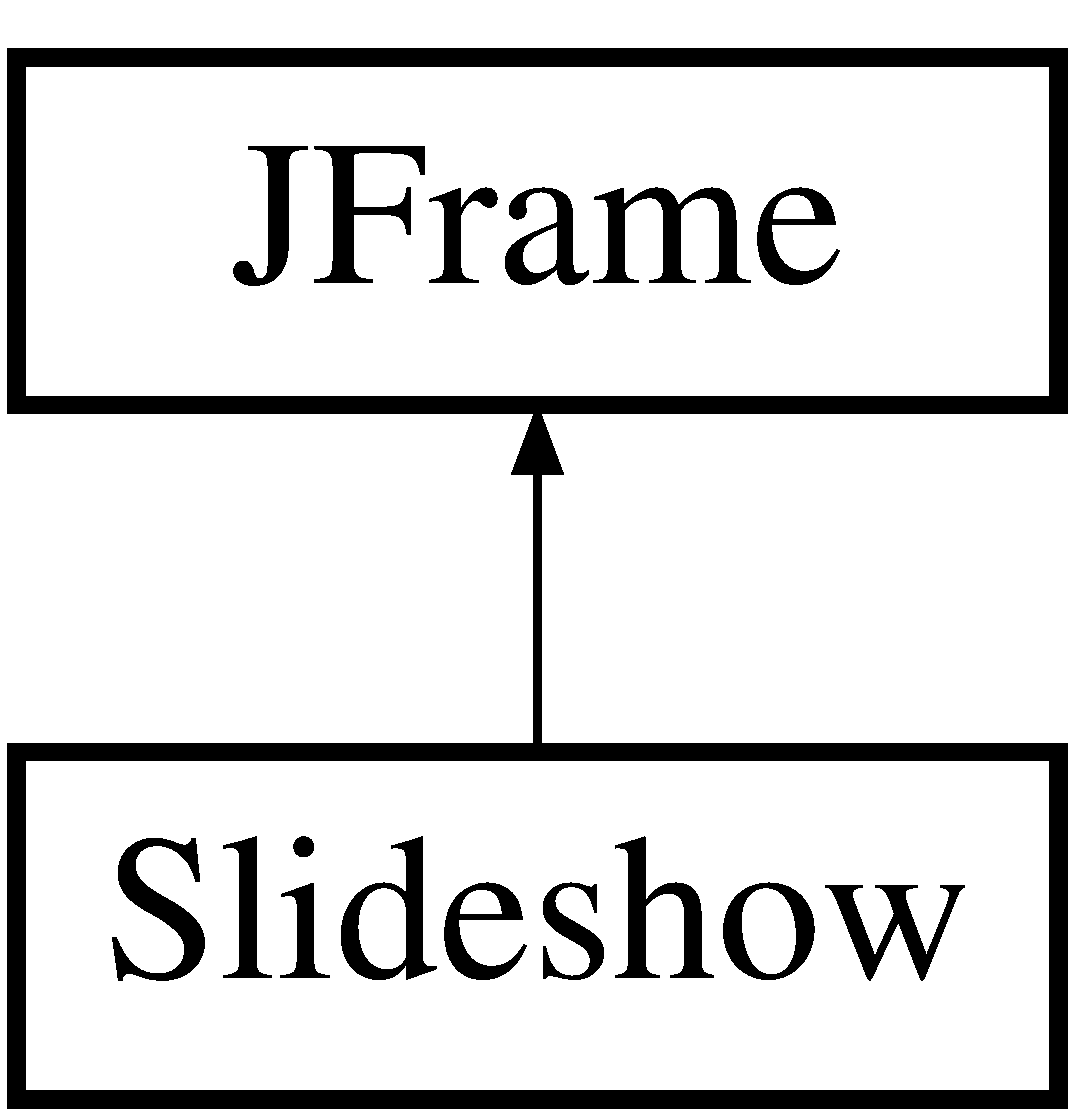
\includegraphics[height=2.000000cm]{class_slideshow}
\end{center}
\end{figure}
\subsection*{Public Member Functions}
\begin{DoxyCompactItemize}
\item 
\hyperlink{class_slideshow_a28bfdbb62ff04edbcf2a6ff4e8277b27}{Slideshow} (String\mbox{[}$\,$\mbox{]}\mbox{[}$\,$\mbox{]} data, \hyperlink{class_dataset}{Dataset} dataset, \hyperlink{class_data_attribute}{Data\-Attribute} setting)
\item 
\hyperlink{class_slideshow_a0fe21ea7ceb1b6a1574729c7cd48f263}{Slideshow} (String\mbox{[}$\,$\mbox{]}\mbox{[}$\,$\mbox{]} data, \hyperlink{class_dataset}{Dataset} dataset, \hyperlink{class_data_attribute}{Data\-Attribute} setting, String\mbox{[}$\,$\mbox{]}\mbox{[}$\,$\mbox{]} second\-Data, \hyperlink{class_dataset}{Dataset} second\-Dataset, \hyperlink{class_data_attribute}{Data\-Attribute} second\-Setting)
\item 
X\-Y\-Z\-Dataset \hyperlink{class_slideshow_a8eabfefadfab208b396dcfef42f052a1}{Create\-Bubble\-Chart\-Dataset} (String\mbox{[}$\,$\mbox{]}\mbox{[}$\,$\mbox{]} data)
\item 
X\-Y\-Z\-Dataset \hyperlink{class_slideshow_a5f490654d036fbc20f7d96acf7cb6d0a}{Create\-Second\-Bubble\-Chart\-Dataset} (String\mbox{[}$\,$\mbox{]}\mbox{[}$\,$\mbox{]} data)
\item 
J\-Free\-Chart \hyperlink{class_slideshow_ab4fdd0457bf5c09167538759056d4dc5}{Create\-Pie\-Chart} (Pie\-Dataset dataset)
\item 
J\-Free\-Chart \hyperlink{class_slideshow_a632f7d55c776bad2fcfa46e5b142fd67}{Create\-Second\-Pie\-Chart} (Pie\-Dataset dataset)
\item 
boolean \hyperlink{class_slideshow_aa6a1c8f9752646edcd00bde9e8b1bccf}{Get\-Pause\-J\-But\-Enabled} ()
\item 
boolean \hyperlink{class_slideshow_a64a069640e3a02812d71c946ba397aaf}{Get\-Resume\-Viz\-J\-But\-Enabled} ()
\end{DoxyCompactItemize}
\subsection*{Static Public Member Functions}
\begin{DoxyCompactItemize}
\item 
static void \hyperlink{class_slideshow_ae461089e26d26eb68382f376b8a457ef}{main} (String\mbox{[}$\,$\mbox{]} args)
\end{DoxyCompactItemize}


\subsection{Detailed Description}
A class that creates a slideshow of a single \hyperlink{interface_chart}{Chart} or two \hyperlink{interface_chart}{Chart} visualizations \textbackslash{} see \hyperlink{_graph_8java}{Graph.\-java}. 

\begin{DoxyDate}{Date}
30/04/13 This class is responsible for making the slideshow It was made using J\-Free\-Chart and following examples on how to set up the charts It uses the \hyperlink{_graph_8java}{Graph.\-java} to return a J\-Free\-Chart 
\end{DoxyDate}


\subsection{Constructor \& Destructor Documentation}
\hypertarget{class_slideshow_a28bfdbb62ff04edbcf2a6ff4e8277b27}{\index{Slideshow@{Slideshow}!Slideshow@{Slideshow}}
\index{Slideshow@{Slideshow}!Slideshow@{Slideshow}}
\subsubsection[{Slideshow}]{\setlength{\rightskip}{0pt plus 5cm}Slideshow.\-Slideshow (
\begin{DoxyParamCaption}
\item[{String}]{data\mbox{[}$\,$\mbox{]}\mbox{[}$\,$\mbox{]}, }
\item[{{\bf Dataset}}]{dataset, }
\item[{{\bf Data\-Attribute}}]{setting}
\end{DoxyParamCaption}
)}}\label{class_slideshow_a28bfdbb62ff04edbcf2a6ff4e8277b27}
creates a constructor taking in the following parameters\-:


\begin{DoxyParams}{Parameters}
{\em String\mbox{[}$\,$\mbox{]}\mbox{[}$\,$\mbox{]}} & data -\/ data used to create the visualisation. \\
\hline
{\em \hyperlink{class_dataset}{Dataset}} & dataset -\/ the dataset used (rows and columns) \\
\hline
{\em \hyperlink{class_data_attribute}{Data\-Attribute}} & setting -\/ Data attributes \\
\hline
\end{DoxyParams}

\begin{DoxyCode}
73                                     \{
74         m\_XYData = data;
75         m\_PieData = data;
76         m\_ScatterData = data; 
77         m\_AreaData = data; 
78         m\_PolarData =data;
79         m\_LineData = data;
80         m\_BubbleData = data;
81         
82         m\_Setting = setting;
83         m\_ChartTitle = setting.\hyperlink{class_data_attribute_ade9747a192ba22fe1020e874bff6a48c}{GetTitle}();
84         m\_XLabel = setting.\hyperlink{class_data_attribute_aecb451704a87d77dd80dbad8a19099d1}{GetAxisLabelX}();
85         m\_YLabel = setting.\hyperlink{class_data_attribute_af5f68794cd0195d42135d5e48120ccc0}{GetAxisLabelY}();
86         m\_Row = dataset.\hyperlink{class_dataset_a91257a605317576e87e1c32e54739e51}{GetNoOfRows}();
87         m\_C1 = setting.\hyperlink{class_data_attribute_a0f4a54973bc44b0526f78bda945dc81b}{GetSelectedXIndex}();
88         m\_C2 = setting.\hyperlink{class_data_attribute_a82e7519853d9f470ea183dd0c39a03d6}{GetSelectedYIndex}();
89         m\_C3 = setting.\hyperlink{class_data_attribute_a802ca8ea739cff583380ea27647250c7}{GetSelectedZIndex}();
90         
91         m\_XMin = setting.\hyperlink{class_data_attribute_afa9da883abc4abad5f64c045de114c50}{GetXAxisMin}();
92         m\_XMax = setting.\hyperlink{class_data_attribute_a81243eb8f7008e05e74b0f3571d2f08d}{GetYAxisMax}();
93         m\_XScale = setting.\hyperlink{class_data_attribute_a5a1de25600487aa958a19ce01151fea4}{GetXAxisScale}();
94         m\_YScale = setting.\hyperlink{class_data_attribute_a95259727ce91efc0e0eaa28487d944c5}{GetYAxisScale}();
95         
96         timerOption = \textcolor{keyword}{new} JFrame(\textcolor{stringliteral}{"Enter a timer"});
97         \textcolor{keywordflow}{while} (m\_OptionPopup = \textcolor{keyword}{true})\{
98             String userOption = JOptionPane.showInputDialog(timerOption, \textcolor{stringliteral}{"Please enter a timer"}
99                     + \textcolor{stringliteral}{"delay in seconds:"});
100               \textcolor{keywordflow}{if} (userOption.matches(\textcolor{stringliteral}{"[0-9]+"}))\{
101                   System.out.println(\textcolor{stringliteral}{"Matches"});
102                   m\_Timer = Integer.parseInt(userOption);
103                   m\_Timer = m\_Timer * m\_Millisecond;
104                   m\_OptionPopup = \textcolor{keyword}{false};
105                   \textcolor{keywordflow}{break};
106               \}
107               System.out.println(\textcolor{stringliteral}{"Not entered match"});
108         \} 
109         
110         CreateXYDataset(m\_XYData);
111         CreatePieChartDataset(m\_PieData);
112         \hyperlink{class_slideshow_a8eabfefadfab208b396dcfef42f052a1}{CreateBubbleChartDataset}(m\_BubbleData);
113         ShowSlideshow( m\_XYDataset, m\_PieChartDataset, m\_XYDataset,
114                 m\_XYDataset, m\_XYDataset, m\_XYDataset, m\_BubbleDataset);
115    \}
\end{DoxyCode}
\hypertarget{class_slideshow_a0fe21ea7ceb1b6a1574729c7cd48f263}{\index{Slideshow@{Slideshow}!Slideshow@{Slideshow}}
\index{Slideshow@{Slideshow}!Slideshow@{Slideshow}}
\subsubsection[{Slideshow}]{\setlength{\rightskip}{0pt plus 5cm}Slideshow.\-Slideshow (
\begin{DoxyParamCaption}
\item[{String}]{data\mbox{[}$\,$\mbox{]}\mbox{[}$\,$\mbox{]}, }
\item[{{\bf Dataset}}]{dataset, }
\item[{{\bf Data\-Attribute}}]{setting, }
\item[{String}]{second\-Data\mbox{[}$\,$\mbox{]}\mbox{[}$\,$\mbox{]}, }
\item[{{\bf Dataset}}]{second\-Dataset, }
\item[{{\bf Data\-Attribute}}]{second\-Setting}
\end{DoxyParamCaption}
)}}\label{class_slideshow_a0fe21ea7ceb1b6a1574729c7cd48f263}
creates a constructor taking in the following parameters\-:


\begin{DoxyParams}{Parameters}
{\em String\mbox{[}$\,$\mbox{]}\mbox{[}$\,$\mbox{]}} & data -\/ data used to create the visualisation. \\
\hline
{\em \hyperlink{class_dataset}{Dataset}} & dataset -\/ the dataset used (rows and columns) \\
\hline
{\em \hyperlink{class_data_attribute}{Data\-Attribute}} & setting -\/ Data attributes \\
\hline
{\em String\mbox{[}$\,$\mbox{]}\mbox{[}$\,$\mbox{]}} & second\-Data -\/ second data used to create the visualisation. \\
\hline
{\em \hyperlink{class_dataset}{Dataset}} & second\-Dataset -\/ the second dataset used (rows and columns) \\
\hline
{\em \hyperlink{class_data_attribute}{Data\-Attribute}} & second\-Setting -\/ Second Data attributes \\
\hline
\end{DoxyParams}

\begin{DoxyCode}
128                                          \{
129 
130           m\_XYData = data;
131           m\_PieData = data;
132           m\_ScatterData = data; 
133           m\_AreaData = data; 
134           m\_PolarData =data;
135           m\_LineData = data;
136           m\_BubbleData = data;
137           m\_SecondXYData = data;
138           m\_SecondPieData = data;
139           m\_SecondScatterData = data; 
140           m\_SecondAreaData = data; 
141           m\_SecondPolarData =data;
142           m\_SecondLineData = data;
143           m\_SecondBubbleData = data;
144           
145           m\_Setting = setting;
146           m\_ChartTitle = setting.\hyperlink{class_data_attribute_ade9747a192ba22fe1020e874bff6a48c}{GetTitle}();
147           m\_XLabel = setting.\hyperlink{class_data_attribute_aecb451704a87d77dd80dbad8a19099d1}{GetAxisLabelX}();
148           m\_YLabel = setting.\hyperlink{class_data_attribute_af5f68794cd0195d42135d5e48120ccc0}{GetAxisLabelY}();
149           m\_Row = dataset.\hyperlink{class_dataset_a91257a605317576e87e1c32e54739e51}{GetNoOfRows}();
150           m\_C1 = setting.\hyperlink{class_data_attribute_a0f4a54973bc44b0526f78bda945dc81b}{GetSelectedXIndex}();
151           m\_C2 = setting.\hyperlink{class_data_attribute_a82e7519853d9f470ea183dd0c39a03d6}{GetSelectedYIndex}();
152           m\_C3 = setting.\hyperlink{class_data_attribute_a802ca8ea739cff583380ea27647250c7}{GetSelectedZIndex}();
153           m\_SecondSetting = secondSetting;
154           m\_SecondChartTitle = secondSetting.\hyperlink{class_data_attribute_a4079522c93025fce7569eaed585f4aeb}{GetSecondTitle}();
155           m\_SecondXLabel = secondSetting.\hyperlink{class_data_attribute_a8ace4cb1fee9e2abeabe3efc9a190c8f}{GetSecondAxisLabelX}();
156           m\_SecondYLabel = secondSetting.\hyperlink{class_data_attribute_a6efb7e067317898feefbbf6bd472b998}{GetSecondAxisLabelY}();
157           m\_SecondRow = secondDataset.\hyperlink{class_dataset_a91257a605317576e87e1c32e54739e51}{GetNoOfRows}();
158           m\_SecondC1 = secondSetting.\hyperlink{class_data_attribute_a7f501790eee650ddf9ac17c4f63a3995}{GetSecondSelectedXIndex}();
159           m\_SecondC2 = secondSetting.\hyperlink{class_data_attribute_a6f61ad05915f4aa31ad3dba00596da64}{GetSecondSelectedYIndex}();
160           m\_SecondC3 = secondSetting.\hyperlink{class_data_attribute_ab8aad538c86b04b4b9a962b7e07e6bc3}{GetSecondSelectedZIndex}();      
161            
162           m\_XMin = setting.\hyperlink{class_data_attribute_afa9da883abc4abad5f64c045de114c50}{GetXAxisMin}();
163           m\_XMax = setting.\hyperlink{class_data_attribute_a81243eb8f7008e05e74b0f3571d2f08d}{GetYAxisMax}();
164           m\_XScale = setting.\hyperlink{class_data_attribute_a5a1de25600487aa958a19ce01151fea4}{GetXAxisScale}();
165           m\_YScale = setting.\hyperlink{class_data_attribute_a95259727ce91efc0e0eaa28487d944c5}{GetYAxisScale}();
166            
167           timerOption  = \textcolor{keyword}{new} JFrame(\textcolor{stringliteral}{"Enter a timer"});
168             \textcolor{keywordflow}{while} (m\_OptionPopup = \textcolor{keyword}{true})\{
169                 String userOption = JOptionPane.showInputDialog(timerOption, \textcolor{stringliteral}{"Please enter a timer"}
170                         + \textcolor{stringliteral}{"delay in seconds:"});
171                   \textcolor{keywordflow}{if} (userOption.matches(\textcolor{stringliteral}{"[0-9]+"}))\{
172                       System.out.println(\textcolor{stringliteral}{"Matches"});
173                       m\_Timer = Integer.parseInt(userOption);
174                       m\_Timer = m\_Timer * m\_Millisecond;
175                       m\_OptionPopup = \textcolor{keyword}{false};
176                       \textcolor{keywordflow}{break};
177                   \}
178                   System.out.println(\textcolor{stringliteral}{"Not entered match"});
179             \} 
180           
181           CreateXYDataset(m\_XYData);
182           CreateSecondXYDataset(m\_SecondXYData);
183           CreatePieChartDataset(m\_PieData);
184           CreateSecondPieChartDataset(m\_SecondPieData);
185           \hyperlink{class_slideshow_a8eabfefadfab208b396dcfef42f052a1}{CreateBubbleChartDataset}(m\_BubbleData);
186           \hyperlink{class_slideshow_a5f490654d036fbc20f7d96acf7cb6d0a}{CreateSecondBubbleChartDataset}(m\_SecondBubbleData);
187           ShowSecondSlideshow(  m\_XYDataset, m\_PieChartDataset, m\_XYDataset,
188                 m\_XYDataset, m\_XYDataset, m\_XYDataset, m\_BubbleDataset,
189                 m\_SecondXYDataset, m\_SecondPieChartDataset,
190                 m\_SecondXYDataset,m\_SecondXYDataset, m\_SecondXYDataset, 
191                 m\_SecondXYDataset, m\_SecondBubbleDataset);
192 
193     \}
\end{DoxyCode}


\subsection{Member Function Documentation}
\hypertarget{class_slideshow_a8eabfefadfab208b396dcfef42f052a1}{\index{Slideshow@{Slideshow}!Create\-Bubble\-Chart\-Dataset@{Create\-Bubble\-Chart\-Dataset}}
\index{Create\-Bubble\-Chart\-Dataset@{Create\-Bubble\-Chart\-Dataset}!Slideshow@{Slideshow}}
\subsubsection[{Create\-Bubble\-Chart\-Dataset}]{\setlength{\rightskip}{0pt plus 5cm}X\-Y\-Z\-Dataset Slideshow.\-Create\-Bubble\-Chart\-Dataset (
\begin{DoxyParamCaption}
\item[{String}]{data\mbox{[}$\,$\mbox{]}\mbox{[}$\,$\mbox{]}}
\end{DoxyParamCaption}
)}}\label{class_slideshow_a8eabfefadfab208b396dcfef42f052a1}
creates an X\-Y\-Z data set for the two selected columns


\begin{DoxyParams}{Parameters}
{\em m\-\_\-data} & -\/ pass the 2d array through \\
\hline
\end{DoxyParams}
\begin{DoxyReturn}{Returns}
dataset -\/ returns the new data set with new values 
\end{DoxyReturn}

\begin{DoxyCode}
268                                                                  \{
269             m\_BubbleDataset = \textcolor{keyword}{new} DefaultXYZDataset();
270             \textcolor{keywordflow}{for}(\textcolor{keywordtype}{int} r = 0; r < m\_Row;r++) \{
271                 \textcolor{keywordtype}{double} xArray[] = \textcolor{keyword}{new} \textcolor{keywordtype}{double}[m\_Row];
272                 \textcolor{keywordtype}{double} yArray[] = \textcolor{keyword}{new} \textcolor{keywordtype}{double}[m\_Row];
273                 \textcolor{keywordtype}{double} zArray[] = \textcolor{keyword}{new} \textcolor{keywordtype}{double}[m\_Row];
274                 
275                 xArray[r] = Double.parseDouble(data[m\_C1][r]);
276                 yArray[r] = Double.parseDouble(data[m\_C2][r]);
277                 zArray[r] = Double.parseDouble(data[m\_C3][r]);
278                 
279                 \textcolor{keywordtype}{double} ad3[][] = \{
280                         xArray, yArray, zArray
281                 \};
282                 m\_BubbleDataset.addSeries(\textcolor{stringliteral}{"Series "} + r, ad3);
283             \}
284             \textcolor{keywordflow}{return} m\_BubbleDataset;
285         \}
\end{DoxyCode}
\hypertarget{class_slideshow_ab4fdd0457bf5c09167538759056d4dc5}{\index{Slideshow@{Slideshow}!Create\-Pie\-Chart@{Create\-Pie\-Chart}}
\index{Create\-Pie\-Chart@{Create\-Pie\-Chart}!Slideshow@{Slideshow}}
\subsubsection[{Create\-Pie\-Chart}]{\setlength{\rightskip}{0pt plus 5cm}J\-Free\-Chart Slideshow.\-Create\-Pie\-Chart (
\begin{DoxyParamCaption}
\item[{Pie\-Dataset}]{dataset}
\end{DoxyParamCaption}
)}}\label{class_slideshow_ab4fdd0457bf5c09167538759056d4dc5}
creates a Pie \hyperlink{interface_chart}{Chart} using the Pie data set and sets the appearance and plot orientation 
\begin{DoxyParams}{Parameters}
{\em Pie\-Dataset} & dataset -\/ the dataset used to make the chart \\
\hline
\end{DoxyParams}
\begin{DoxyReturn}{Returns}
J\-Free\-Chart chart -\/ the chart 
\end{DoxyReturn}

\begin{DoxyCode}
396                                                            \{
397         
398         JFreeChart chart = ChartFactory.createPieChart3D( 
399                 m\_ChartTitle,
400             dataset, \textcolor{keyword}{true},                          
401             \textcolor{keyword}{true}, \textcolor{keyword}{false} );
402         
403         \textcolor{comment}{//xyPlot = chart.getXYPlot();}
404         plotChart  = ( PiePlot3D ) chart.getPlot();      
405         plotChart.setStartAngle( START\_ANGLE );
406         plotChart.setDirection( Rotation.CLOCKWISE ); 
407         plotChart.setForegroundAlpha(TRANSPARENCY); 
408         \textcolor{keywordflow}{return} chart;       
409     \}
\end{DoxyCode}
\hypertarget{class_slideshow_a5f490654d036fbc20f7d96acf7cb6d0a}{\index{Slideshow@{Slideshow}!Create\-Second\-Bubble\-Chart\-Dataset@{Create\-Second\-Bubble\-Chart\-Dataset}}
\index{Create\-Second\-Bubble\-Chart\-Dataset@{Create\-Second\-Bubble\-Chart\-Dataset}!Slideshow@{Slideshow}}
\subsubsection[{Create\-Second\-Bubble\-Chart\-Dataset}]{\setlength{\rightskip}{0pt plus 5cm}X\-Y\-Z\-Dataset Slideshow.\-Create\-Second\-Bubble\-Chart\-Dataset (
\begin{DoxyParamCaption}
\item[{String}]{data\mbox{[}$\,$\mbox{]}\mbox{[}$\,$\mbox{]}}
\end{DoxyParamCaption}
)}}\label{class_slideshow_a5f490654d036fbc20f7d96acf7cb6d0a}
creates a second X\-Y\-Z data set for the two selected columns


\begin{DoxyParams}{Parameters}
{\em m\-\_\-data} & -\/ pass the 2d array through \\
\hline
\end{DoxyParams}
\begin{DoxyReturn}{Returns}
dataset -\/ returns the new data set with new values 
\end{DoxyReturn}

\begin{DoxyCode}
292                                                                        \{
293             m\_SecondBubbleDataset = \textcolor{keyword}{new} DefaultXYZDataset();
294             \textcolor{keywordflow}{for}(\textcolor{keywordtype}{int} r = 0; r < m\_SecondRow;r++) \{
295                 \textcolor{keywordtype}{double} xArray[] = \textcolor{keyword}{new} \textcolor{keywordtype}{double}[m\_SecondRow];
296                 \textcolor{keywordtype}{double} yArray[] = \textcolor{keyword}{new} \textcolor{keywordtype}{double}[m\_SecondRow];
297                 \textcolor{keywordtype}{double} zArray[] = \textcolor{keyword}{new} \textcolor{keywordtype}{double}[m\_SecondRow];
298                 
299                 xArray[r] = Double.parseDouble(data[m\_SecondC1][r]);
300                 yArray[r] = Double.parseDouble(data[m\_SecondC2][r]);
301                 zArray[r] = Double.parseDouble(data[m\_SecondC3][r]);
302                 
303                 \textcolor{keywordtype}{double} ad3[][] = \{
304                         xArray, yArray, zArray
305                 \};
306                 m\_SecondBubbleDataset.addSeries(\textcolor{stringliteral}{"Series "} + r, ad3);
307             \}
308             \textcolor{keywordflow}{return} m\_SecondBubbleDataset;
309         \}
\end{DoxyCode}
\hypertarget{class_slideshow_a632f7d55c776bad2fcfa46e5b142fd67}{\index{Slideshow@{Slideshow}!Create\-Second\-Pie\-Chart@{Create\-Second\-Pie\-Chart}}
\index{Create\-Second\-Pie\-Chart@{Create\-Second\-Pie\-Chart}!Slideshow@{Slideshow}}
\subsubsection[{Create\-Second\-Pie\-Chart}]{\setlength{\rightskip}{0pt plus 5cm}J\-Free\-Chart Slideshow.\-Create\-Second\-Pie\-Chart (
\begin{DoxyParamCaption}
\item[{Pie\-Dataset}]{dataset}
\end{DoxyParamCaption}
)}}\label{class_slideshow_a632f7d55c776bad2fcfa46e5b142fd67}
creates a second Pie \hyperlink{interface_chart}{Chart} using the Pie data set and sets the appearance and plot orientation 
\begin{DoxyParams}{Parameters}
{\em Pie\-Dataset} & dataset -\/ the dataset used to make the chart \\
\hline
\end{DoxyParams}
\begin{DoxyReturn}{Returns}
J\-Free\-Chart chart -\/ the chart 
\end{DoxyReturn}

\begin{DoxyCode}
416                                                                  \{
417         
418         JFreeChart chart = ChartFactory.createPieChart3D( 
419                 m\_SecondChartTitle,
420             dataset, \textcolor{keyword}{true},                          
421             \textcolor{keyword}{true}, \textcolor{keyword}{false} );
422         
423         \textcolor{comment}{//xyPlot = chart.getXYPlot();}
424         plotSecondChart  = ( PiePlot3D ) chart.getPlot();      
425         plotSecondChart.setStartAngle( START\_ANGLE );
426         plotSecondChart.setDirection( Rotation.CLOCKWISE ); 
427         plotSecondChart.setForegroundAlpha(TRANSPARENCY); 
428         \textcolor{keywordflow}{return} chart;       
429     \}
\end{DoxyCode}
\hypertarget{class_slideshow_aa6a1c8f9752646edcd00bde9e8b1bccf}{\index{Slideshow@{Slideshow}!Get\-Pause\-J\-But\-Enabled@{Get\-Pause\-J\-But\-Enabled}}
\index{Get\-Pause\-J\-But\-Enabled@{Get\-Pause\-J\-But\-Enabled}!Slideshow@{Slideshow}}
\subsubsection[{Get\-Pause\-J\-But\-Enabled}]{\setlength{\rightskip}{0pt plus 5cm}boolean Slideshow.\-Get\-Pause\-J\-But\-Enabled (
\begin{DoxyParamCaption}
{}
\end{DoxyParamCaption}
)}}\label{class_slideshow_aa6a1c8f9752646edcd00bde9e8b1bccf}
Method to see if the pause button has been selected \begin{DoxyReturn}{Returns}
m\-\_\-\-Pause 
\end{DoxyReturn}

\begin{DoxyCode}
1255                                          \{
1256         \textcolor{keywordflow}{return} m\_Pause;
1257     \}
\end{DoxyCode}
\hypertarget{class_slideshow_a64a069640e3a02812d71c946ba397aaf}{\index{Slideshow@{Slideshow}!Get\-Resume\-Viz\-J\-But\-Enabled@{Get\-Resume\-Viz\-J\-But\-Enabled}}
\index{Get\-Resume\-Viz\-J\-But\-Enabled@{Get\-Resume\-Viz\-J\-But\-Enabled}!Slideshow@{Slideshow}}
\subsubsection[{Get\-Resume\-Viz\-J\-But\-Enabled}]{\setlength{\rightskip}{0pt plus 5cm}boolean Slideshow.\-Get\-Resume\-Viz\-J\-But\-Enabled (
\begin{DoxyParamCaption}
{}
\end{DoxyParamCaption}
)}}\label{class_slideshow_a64a069640e3a02812d71c946ba397aaf}
Method to see if the resume button has been selected \begin{DoxyReturn}{Returns}
m\-\_\-\-Resume 
\end{DoxyReturn}

\begin{DoxyCode}
1262                                              \{
1263         \textcolor{keywordflow}{return} m\_ResumeButton.isEnabled();
1264     \}   
\end{DoxyCode}
\hypertarget{class_slideshow_ae461089e26d26eb68382f376b8a457ef}{\index{Slideshow@{Slideshow}!main@{main}}
\index{main@{main}!Slideshow@{Slideshow}}
\subsubsection[{main}]{\setlength{\rightskip}{0pt plus 5cm}static void Slideshow.\-main (
\begin{DoxyParamCaption}
\item[{String\mbox{[}$\,$\mbox{]}}]{args}
\end{DoxyParamCaption}
)\hspace{0.3cm}{\ttfamily [static]}}}\label{class_slideshow_ae461089e26d26eb68382f376b8a457ef}

\begin{DoxyCode}
1265                                            \{        
1266             
1267     \}
\end{DoxyCode}


The documentation for this class was generated from the following file\-:\begin{DoxyCompactItemize}
\item 
\hyperlink{_slideshow_8java}{Slideshow.\-java}\end{DoxyCompactItemize}

\hypertarget{class_status_j_panel}{\section{Status\-J\-Panel Class Reference}
\label{class_status_j_panel}\index{Status\-J\-Panel@{Status\-J\-Panel}}
}


This class will display the status of the application.  


Inheritance diagram for Status\-J\-Panel\-:\begin{figure}[H]
\begin{center}
\leavevmode
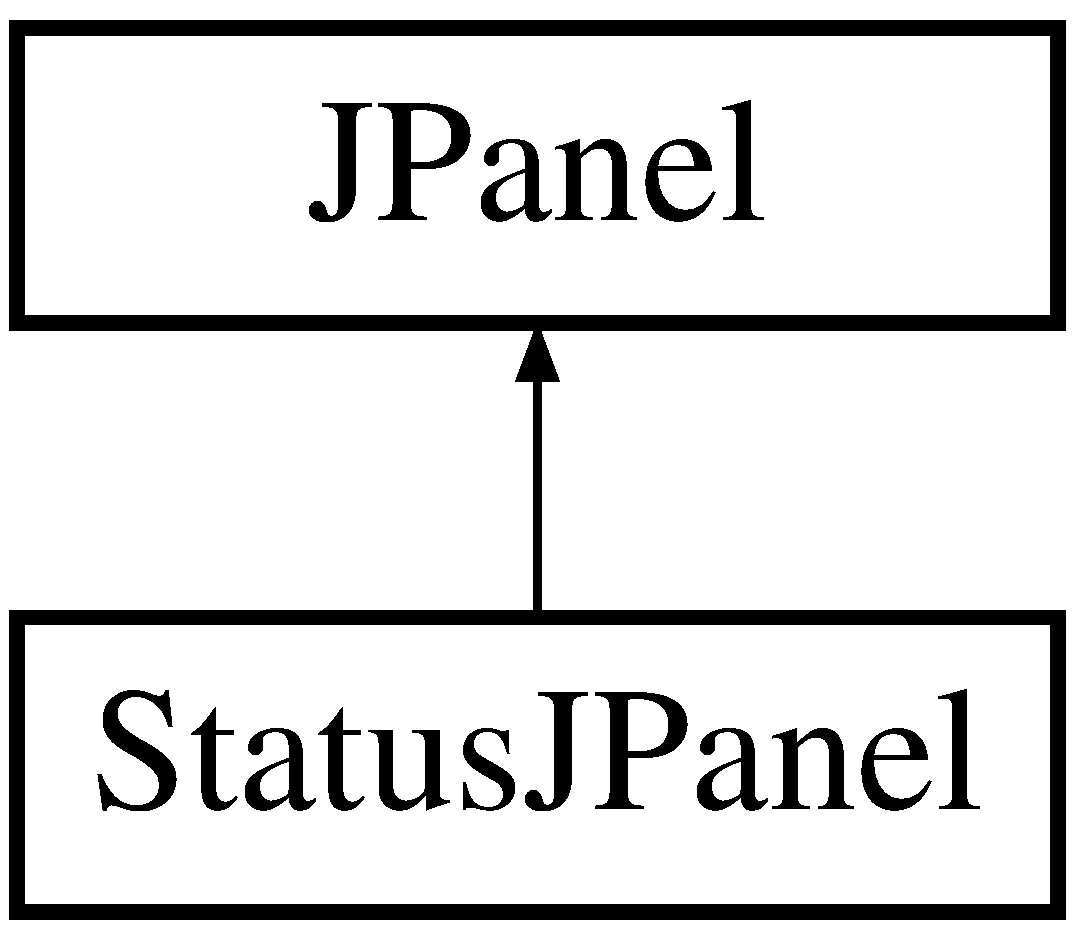
\includegraphics[height=2.000000cm]{class_status_j_panel}
\end{center}
\end{figure}
\subsection*{Public Member Functions}
\begin{DoxyCompactItemize}
\item 
boolean \hyperlink{class_status_j_panel_ac601eae1536e1a412c71f383cd116610}{Set\-Status} (String status)
\item 
String \hyperlink{class_status_j_panel_afea138c52207657b5b3b555ce1a70e42}{Get\-Status} ()
\item 
\hyperlink{class_status_j_panel_a2ec0b292761d595f99ac7293398ae97a}{Status\-J\-Panel} ()
\item 
boolean \hyperlink{class_status_j_panel_a80d2f3a1eba1516b449115fb8464cfac}{Set\-B\-V} (\hyperlink{class_bob_viz}{Bob\-Viz} bv)
\end{DoxyCompactItemize}


\subsection{Detailed Description}
This class will display the status of the application. 

\begin{DoxyDate}{Date}
-\/02/03/2013 
\end{DoxyDate}
\begin{DoxySeeAlso}{See Also}
\hyperlink{_bob_viz_8java}{Bob\-Viz.\-java} 
\end{DoxySeeAlso}


\subsection{Constructor \& Destructor Documentation}
\hypertarget{class_status_j_panel_a2ec0b292761d595f99ac7293398ae97a}{\index{Status\-J\-Panel@{Status\-J\-Panel}!Status\-J\-Panel@{Status\-J\-Panel}}
\index{Status\-J\-Panel@{Status\-J\-Panel}!StatusJPanel@{Status\-J\-Panel}}
\subsubsection[{Status\-J\-Panel}]{\setlength{\rightskip}{0pt plus 5cm}Status\-J\-Panel.\-Status\-J\-Panel (
\begin{DoxyParamCaption}
{}
\end{DoxyParamCaption}
)}}\label{class_status_j_panel_a2ec0b292761d595f99ac7293398ae97a}

\begin{DoxyCode}
40                           \{
41         \textcolor{comment}{/* set dimensions of StatusJPanel */}
42         Dimension size = getPreferredSize();
43         size.height = PAN\_HEIGHT;
44         \textcolor{comment}{/* set new layout for FlowLayout */}
45         setLayout( \textcolor{keyword}{new} FlowLayout( FlowLayout.LEFT ) );
46         \textcolor{comment}{/* set new size */}
47         setPreferredSize( size );
48         \textcolor{comment}{/* set new background colour */}
49         setBackground( \textcolor{keyword}{new} Color( BACK\_COL, BACK\_COL, BACK\_COL ) );
50         setBorder( BorderFactory.createMatteBorder( BORD\_TOP, BORD\_BOT, 
51                 BORD\_LEFT, BORD\_RIGHT, Color.LIGHT\_GRAY ) );
52         \textcolor{comment}{/* add status label to new StatusJPanel */}
53         add( statusJLab );
54     \}
\end{DoxyCode}


\subsection{Member Function Documentation}
\hypertarget{class_status_j_panel_afea138c52207657b5b3b555ce1a70e42}{\index{Status\-J\-Panel@{Status\-J\-Panel}!Get\-Status@{Get\-Status}}
\index{Get\-Status@{Get\-Status}!StatusJPanel@{Status\-J\-Panel}}
\subsubsection[{Get\-Status}]{\setlength{\rightskip}{0pt plus 5cm}String Status\-J\-Panel.\-Get\-Status (
\begin{DoxyParamCaption}
{}
\end{DoxyParamCaption}
)}}\label{class_status_j_panel_afea138c52207657b5b3b555ce1a70e42}
\begin{DoxyReturn}{Returns}
String m\-\_\-\-Status -\/a variable which stores the current status of the program. 
\end{DoxyReturn}

\begin{DoxyCode}
36                               \{
37         \textcolor{keywordflow}{return} m\_Status;
38     \}
\end{DoxyCode}
\hypertarget{class_status_j_panel_a80d2f3a1eba1516b449115fb8464cfac}{\index{Status\-J\-Panel@{Status\-J\-Panel}!Set\-B\-V@{Set\-B\-V}}
\index{Set\-B\-V@{Set\-B\-V}!StatusJPanel@{Status\-J\-Panel}}
\subsubsection[{Set\-B\-V}]{\setlength{\rightskip}{0pt plus 5cm}boolean Status\-J\-Panel.\-Set\-B\-V (
\begin{DoxyParamCaption}
\item[{{\bf Bob\-Viz}}]{bv}
\end{DoxyParamCaption}
)}}\label{class_status_j_panel_a80d2f3a1eba1516b449115fb8464cfac}

\begin{DoxyParams}{Parameters}
{\em bv} & -\/ a \hyperlink{class_bob_viz}{Bob\-Viz} object \\
\hline
\end{DoxyParams}
\begin{DoxyReturn}{Returns}
T\-R\-U\-E on success 
\end{DoxyReturn}

\begin{DoxyCode}
60                                       \{
61         \textcolor{keywordtype}{boolean} test = \textcolor{keyword}{true};
62         \textcolor{keywordflow}{if}( ( test == \textcolor{keyword}{true} ) && ( bv == null ) ) \{
63             System.err.println( \textcolor{stringliteral}{"StatusJPanel::SetBV() ***Warning, object"}
64                     + \textcolor{stringliteral}{"is null. Value sent: "} + bv );
65         \} \textcolor{keywordflow}{else} \textcolor{keywordflow}{if} ( test == \textcolor{keyword}{true} ) \{
66             System.out.println( \textcolor{stringliteral}{"StatusJPanel::SetBV() Object is valid. Value"}
67                     + \textcolor{stringliteral}{"sent: "} + bv );
68         \}
69         m\_BV = bv;
70         \textcolor{keywordflow}{return} \textcolor{keyword}{true};
71     \}
\end{DoxyCode}
\hypertarget{class_status_j_panel_ac601eae1536e1a412c71f383cd116610}{\index{Status\-J\-Panel@{Status\-J\-Panel}!Set\-Status@{Set\-Status}}
\index{Set\-Status@{Set\-Status}!StatusJPanel@{Status\-J\-Panel}}
\subsubsection[{Set\-Status}]{\setlength{\rightskip}{0pt plus 5cm}boolean Status\-J\-Panel.\-Set\-Status (
\begin{DoxyParamCaption}
\item[{String}]{status}
\end{DoxyParamCaption}
)}}\label{class_status_j_panel_ac601eae1536e1a412c71f383cd116610}
This method updates the status of the program. Other classes will call this method to update the status which will inform the user. 
\begin{DoxyParams}{Parameters}
{\em status} & -\/ the current status. \\
\hline
\end{DoxyParams}
\begin{DoxyReturn}{Returns}
boolen true if successful 
\end{DoxyReturn}

\begin{DoxyCode}
26                                               \{
27         m\_Status = status;
28         statusJLab.setText( \textcolor{stringliteral}{"Status: "} + \hyperlink{class_status_j_panel_afea138c52207657b5b3b555ce1a70e42}{GetStatus}() );
29         \textcolor{keywordflow}{return} \textcolor{keyword}{true};
30     \}
\end{DoxyCode}


The documentation for this class was generated from the following file\-:\begin{DoxyCompactItemize}
\item 
\hyperlink{_status_j_panel_8java}{Status\-J\-Panel.\-java}\end{DoxyCompactItemize}

\hypertarget{class_table}{\section{Table Class Reference}
\label{class_table}\index{Table@{Table}}
}


A simple class that displays data in a table visualisation.  


Inheritance diagram for Table\-:\begin{figure}[H]
\begin{center}
\leavevmode
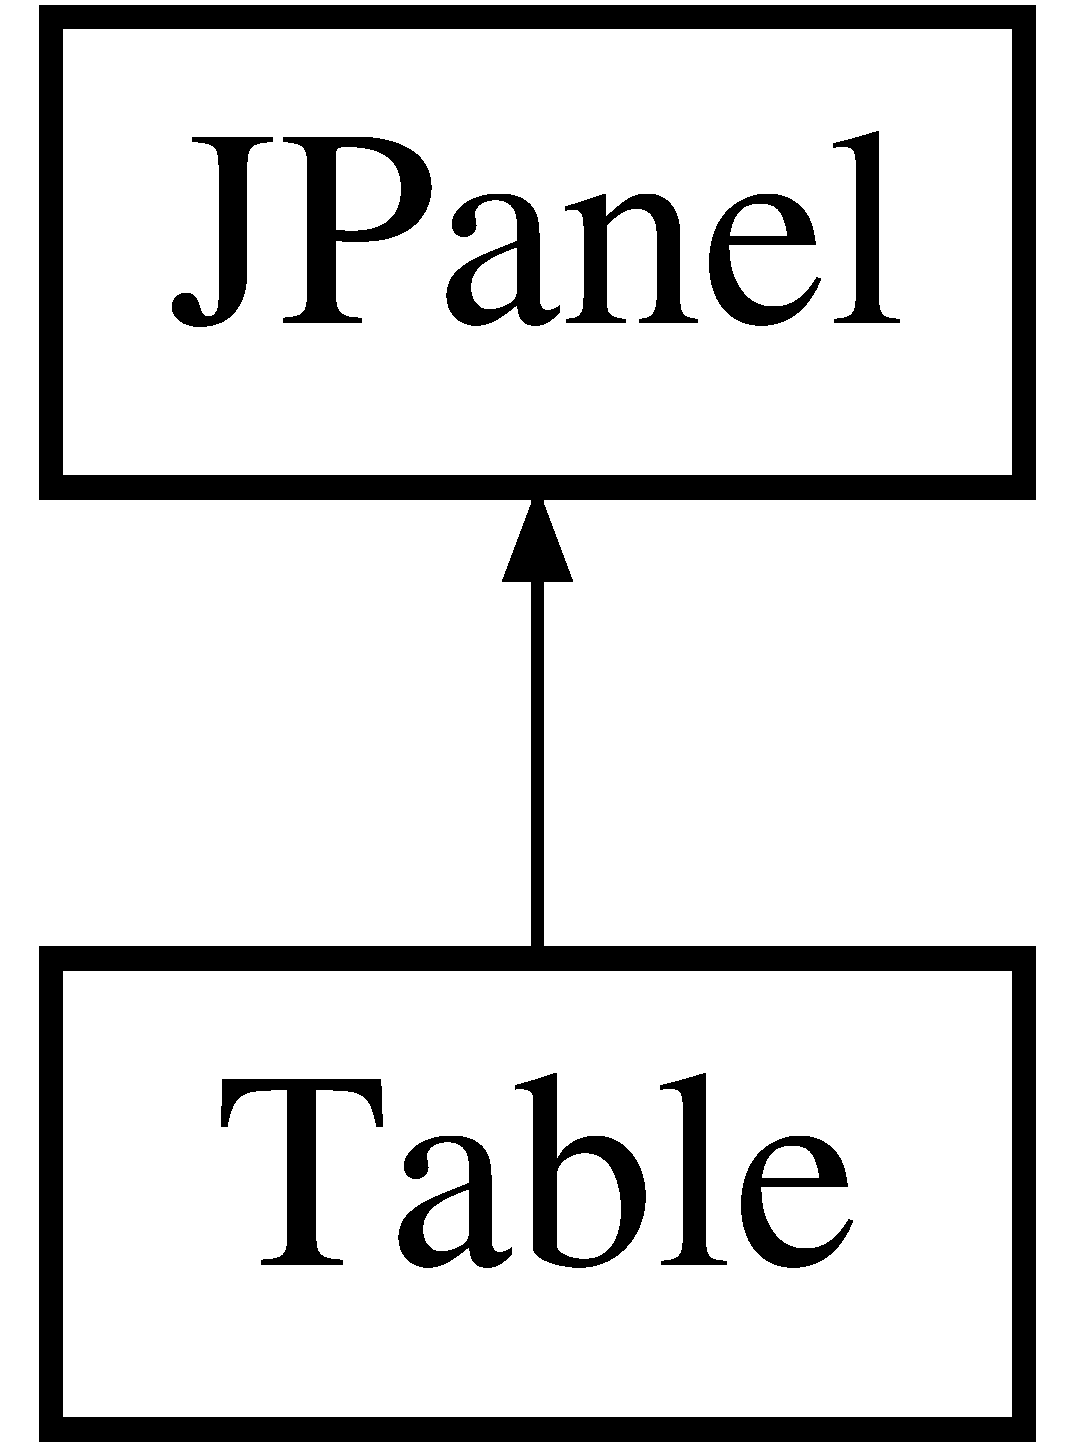
\includegraphics[height=2.000000cm]{class_table}
\end{center}
\end{figure}
\subsection*{Public Member Functions}
\begin{DoxyCompactItemize}
\item 
\hyperlink{class_table_a55d3afc76dfd94c753fc7e8086c0c02d}{Table} (String\mbox{[}$\,$\mbox{]}\mbox{[}$\,$\mbox{]} m\-\_\-data, String\mbox{[}$\,$\mbox{]} m\-\_\-headers, String table\-Title)
\item 
\hyperlink{class_table_ac32e2c58f437c8ee3d576766d2a0f5f8}{Table} (String\mbox{[}$\,$\mbox{]}\mbox{[}$\,$\mbox{]} m\-\_\-data, String\mbox{[}$\,$\mbox{]} m\-\_\-header, String table\-Title, String\mbox{[}$\,$\mbox{]}\mbox{[}$\,$\mbox{]} m\-\_\-second\-Data, String\mbox{[}$\,$\mbox{]} m\-\_\-second\-Header, String second\-Table\-Title)
\end{DoxyCompactItemize}
\subsection*{Static Public Member Functions}
\begin{DoxyCompactItemize}
\item 
static void \hyperlink{class_table_a1484279c07eaa8220aa52c7036d6a2cf}{main} (String\mbox{[}$\,$\mbox{]} args)
\end{DoxyCompactItemize}


\subsection{Detailed Description}
A simple class that displays data in a table visualisation. 

\begin{DoxyDate}{Date}
30/04/2013 
\end{DoxyDate}


\subsection{Constructor \& Destructor Documentation}
\hypertarget{class_table_a55d3afc76dfd94c753fc7e8086c0c02d}{\index{Table@{Table}!Table@{Table}}
\index{Table@{Table}!Table@{Table}}
\subsubsection[{Table}]{\setlength{\rightskip}{0pt plus 5cm}Table.\-Table (
\begin{DoxyParamCaption}
\item[{String}]{m\-\_\-data\mbox{[}$\,$\mbox{]}\mbox{[}$\,$\mbox{]}, }
\item[{String\mbox{[}$\,$\mbox{]}}]{m\-\_\-headers, }
\item[{String}]{table\-Title}
\end{DoxyParamCaption}
)}}\label{class_table_a55d3afc76dfd94c753fc7e8086c0c02d}

\begin{DoxyParams}{Parameters}
{\em m\-\_\-data} & -\/ the data to be passed from users to the table \\
\hline
{\em m\-\_\-headers} & -\/ the headers to be passed to the table \\
\hline
{\em table\-Title} & -\/ the title to be passed to the table \\
\hline
\end{DoxyParams}
Instantiate a table taking in specific data from users

Create a J\-Scroll\-Pane which adds the J\-Table 
\begin{DoxyCode}
20                                                                              \{
22     JTable table = \textcolor{keyword}{new} JTable( m\_data, m\_headers );
23     table.setBorder( BorderFactory.createLineBorder( Color.gray ) );
24         JLabel title = \textcolor{keyword}{new} JLabel( tableTitle );
25        
26         JPanel panel = \textcolor{keyword}{new} JPanel();
27         panel.add( title );
29         JScrollPane scrollPane = \textcolor{keyword}{new} JScrollPane( table );
30         scrollPane.setBorder( BorderFactory.createEmptyBorder() );
31         JPanel tableJPan = \textcolor{keyword}{new} JPanel();
32         JButton disabledBut = \textcolor{keyword}{new} JButton( \textcolor{stringliteral}{"Change colour"} );
33         disabledBut.setEnabled( \textcolor{keyword}{false} );
34         tableJPan.add( scrollPane );
35         
36         JFrame test = \textcolor{keyword}{new} JFrame();
37         test.setLayout( \textcolor{keyword}{new} BorderLayout() );
38         test.setSize( WIDTH\_FRAME, HEIGHT\_FRAME );
39         test.setTitle( \textcolor{stringliteral}{"Table"} );
40         test.setDefaultCloseOperation( JFrame.DISPOSE\_ON\_CLOSE );
41         test.add( tableJPan, BorderLayout.CENTER );
42         test.add( panel, BorderLayout.NORTH );
43         test.setVisible( \textcolor{keyword}{true} );
44     \}
\end{DoxyCode}
\hypertarget{class_table_ac32e2c58f437c8ee3d576766d2a0f5f8}{\index{Table@{Table}!Table@{Table}}
\index{Table@{Table}!Table@{Table}}
\subsubsection[{Table}]{\setlength{\rightskip}{0pt plus 5cm}Table.\-Table (
\begin{DoxyParamCaption}
\item[{String}]{m\-\_\-data\mbox{[}$\,$\mbox{]}\mbox{[}$\,$\mbox{]}, }
\item[{String\mbox{[}$\,$\mbox{]}}]{m\-\_\-header, }
\item[{String}]{table\-Title, }
\item[{Stringm\-\_\-second\-Data}]{\mbox{[}$\,$\mbox{]}\mbox{[}$\,$\mbox{]}, }
\item[{String\mbox{[}$\,$\mbox{]}}]{m\-\_\-second\-Header, }
\item[{String}]{second\-Table\-Title}
\end{DoxyParamCaption}
)}}\label{class_table_ac32e2c58f437c8ee3d576766d2a0f5f8}

\begin{DoxyParams}{Parameters}
{\em m\-\_\-data} & -\/ the data to be passed from users to the table \\
\hline
{\em m\-\_\-header} & -\/ the headers to be passed to the table \\
\hline
{\em table\-Title} & -\/ the title to be passed to the table \\
\hline
{\em m\-\_\-second\-Data} & -\/ the second C\-S\-V data to be passed from users to the table \\
\hline
{\em m\-\_\-second\-Header} & -\/ the second headers to be passed to the table \\
\hline
{\em second\-Table\-Title} & -\/ the second title to be passed to the table \\
\hline
\end{DoxyParams}
Create a J\-Scroll\-Pane which adds the J\-Table 
\begin{DoxyCode}
55                                                                                              \{
56         JTable table = \textcolor{keyword}{new} JTable( m\_data, m\_header );
57         table.setBorder( BorderFactory.createLineBorder( Color.gray ) );
58             
59             JLabel title = \textcolor{keyword}{new} JLabel( tableTitle + \textcolor{stringliteral}{"      "} +
60                     \textcolor{stringliteral}{"                                      "} +
61                     \textcolor{stringliteral}{"                                      "} +
62                     secondTableTitle );
63             JPanel panel = \textcolor{keyword}{new} JPanel();
64             panel.add( title );
65             
67             JScrollPane scrollPane = \textcolor{keyword}{new} JScrollPane( table );
68             scrollPane.setBorder( BorderFactory.createEmptyBorder() );
69             JPanel tableJPan = \textcolor{keyword}{new} JPanel();
70             JButton disabledBut = \textcolor{keyword}{new} JButton( \textcolor{stringliteral}{"Change colour"} );
71             disabledBut.setEnabled( \textcolor{keyword}{false} );
72             tableJPan.add( scrollPane );
73            
74         JTable secondTable = \textcolor{keyword}{new} JTable( m\_secondData, m\_secondHeader );
75         secondTable.setBorder( BorderFactory.createLineBorder( Color.gray ) );
76             
77             JScrollPane secondScrollPane = \textcolor{keyword}{new} JScrollPane( secondTable );
78             secondScrollPane.setBorder( BorderFactory.createEmptyBorder() );
79             JPanel secondTableJPan = \textcolor{keyword}{new} JPanel();
80             JButton secondDisabledBut = \textcolor{keyword}{new} JButton( \textcolor{stringliteral}{"Change colour"} );
81             secondDisabledBut.setEnabled( \textcolor{keyword}{false} );
82             secondTableJPan.add( secondScrollPane );
83            
84         JFrame test = \textcolor{keyword}{new} JFrame();
85         test.setLayout( \textcolor{keyword}{new} BorderLayout() );
86         test.setSize( SECOND\_WIDTH\_FRAME, SECOND\_HEIGHT\_FRAME );
87         test.setTitle( \textcolor{stringliteral}{"Table with two csv files"} );
88         test.setDefaultCloseOperation( JFrame.DISPOSE\_ON\_CLOSE );
89         test.add( tableJPan, BorderLayout.WEST);
90         test.add( panel , BorderLayout.NORTH);
91         test.add( secondTableJPan, BorderLayout.EAST);        
92         test.setVisible( \textcolor{keyword}{true} );
93             
94        
95     \}
\end{DoxyCode}


\subsection{Member Function Documentation}
\hypertarget{class_table_a1484279c07eaa8220aa52c7036d6a2cf}{\index{Table@{Table}!main@{main}}
\index{main@{main}!Table@{Table}}
\subsubsection[{main}]{\setlength{\rightskip}{0pt plus 5cm}static void Table.\-main (
\begin{DoxyParamCaption}
\item[{String\mbox{[}$\,$\mbox{]}}]{args}
\end{DoxyParamCaption}
)\hspace{0.3cm}{\ttfamily [static]}}}\label{class_table_a1484279c07eaa8220aa52c7036d6a2cf}

\begin{DoxyCode}
97                                            \{
98  
99         String array[][] = arrayTest;
100         String array1[] = \{\textcolor{stringliteral}{"header1"},\textcolor{stringliteral}{"header2"},\textcolor{stringliteral}{"header3"},\textcolor{stringliteral}{"header4"}\};
101         \hyperlink{class_table}{Table} Tabletest = \textcolor{keyword}{new} \hyperlink{class_table_a55d3afc76dfd94c753fc7e8086c0c02d}{Table}(array, array1, \textcolor{stringliteral}{"Test Table"});
102     
103         String arraya[][] = arrayTest;
104         String array2[] = \{\textcolor{stringliteral}{"header1"},\textcolor{stringliteral}{"header2"},\textcolor{stringliteral}{"header3"},\textcolor{stringliteral}{"header4"}\};
105         String arrayb[][] = arrayTest2;
106         String array3[] = \{\textcolor{stringliteral}{"header5"},\textcolor{stringliteral}{"header6"},\textcolor{stringliteral}{"header7"},\textcolor{stringliteral}{"header8"}\};
107         
108         \hyperlink{class_table}{Table} Tabletest2 = \textcolor{keyword}{new} \hyperlink{class_table_a55d3afc76dfd94c753fc7e8086c0c02d}{Table}(arraya, array2, \textcolor{stringliteral}{"Test Table 1"}, arrayb, array3, \textcolor{stringliteral}{"Test Table
       2"});
109     \}
\end{DoxyCode}


The documentation for this class was generated from the following file\-:\begin{DoxyCompactItemize}
\item 
\hyperlink{_table_8java}{Table.\-java}\end{DoxyCompactItemize}

\hypertarget{class_visualisation}{\section{Visualisation Class Reference}
\label{class_visualisation}\index{Visualisation@{Visualisation}}
}


A class that displays specific data in a Column \hyperlink{interface_chart}{Chart} visualiser.  


Inheritance diagram for Visualisation\-:\begin{figure}[H]
\begin{center}
\leavevmode
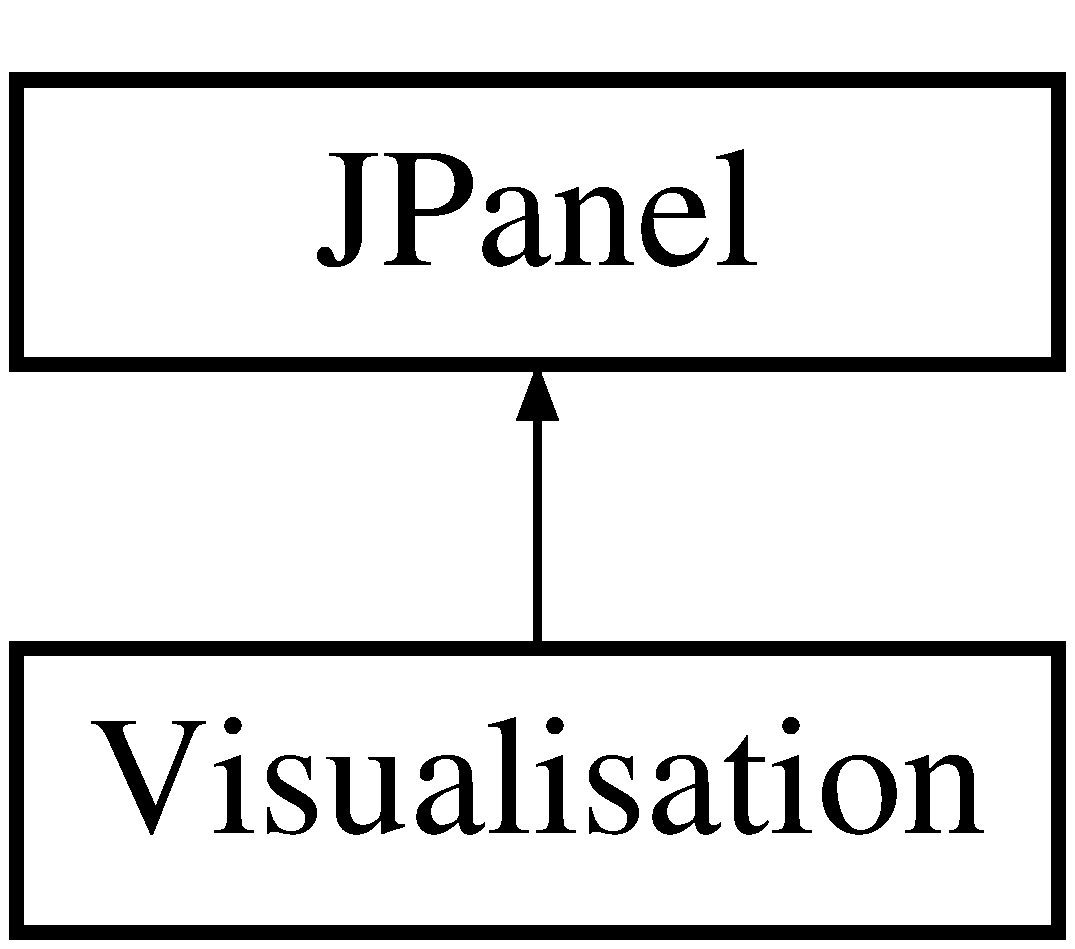
\includegraphics[height=2.000000cm]{class_visualisation}
\end{center}
\end{figure}
\subsection*{Public Member Functions}
\begin{DoxyCompactItemize}
\item 
\hyperlink{class_column_chart}{Column\-Chart} \hyperlink{class_visualisation_aa3b086e3056acc670676337341548c35}{Get\-Col\-Chart} ()
\item 
boolean \hyperlink{class_visualisation_ac5cdad052bcbab9babaa5ecdfd2427ea}{Set\-Col\-Chart} (String\mbox{[}$\,$\mbox{]}\mbox{[}$\,$\mbox{]} data, \hyperlink{class_dataset}{Dataset} dataset, \hyperlink{class_data_attribute}{Data\-Attribute} setting)
\item 
boolean \hyperlink{class_visualisation_a118d994f12e22a0dea33925695851941}{Set\-Col\-Chart} (String\mbox{[}$\,$\mbox{]}\mbox{[}$\,$\mbox{]} data, \hyperlink{class_dataset}{Dataset} dataset, \hyperlink{class_data_attribute}{Data\-Attribute} setting, String\mbox{[}$\,$\mbox{]}\mbox{[}$\,$\mbox{]} second\-Data, \hyperlink{class_dataset}{Dataset} second\-Dataset, \hyperlink{class_data_attribute}{Data\-Attribute} second\-Setting)
\item 
\hyperlink{class_pie_chart}{Pie\-Chart} \hyperlink{class_visualisation_abe4f0b9c1cd424c7de4277934b21a99d}{Get\-Viz\-Pie\-Chart} ()
\item 
boolean \hyperlink{class_visualisation_ae459b89156fb23c84a2d5fe9ffb08f24}{Set\-Viz\-Pie\-Chart} (String\mbox{[}$\,$\mbox{]}\mbox{[}$\,$\mbox{]} data, \hyperlink{class_dataset}{Dataset} dataset, \hyperlink{class_data_attribute}{Data\-Attribute} setting)
\item 
boolean \hyperlink{class_visualisation_a2a1211b45fd9b1018191e6207d71f82a}{Set\-Viz\-Pie\-Chart} (String\mbox{[}$\,$\mbox{]}\mbox{[}$\,$\mbox{]} data, \hyperlink{class_dataset}{Dataset} dataset, \hyperlink{class_data_attribute}{Data\-Attribute} setting, String\mbox{[}$\,$\mbox{]}\mbox{[}$\,$\mbox{]} second\-Data, \hyperlink{class_dataset}{Dataset} second\-Dataset, \hyperlink{class_data_attribute}{Data\-Attribute} second\-Setting)
\item 
\hyperlink{class_area_chart}{Area\-Chart} \hyperlink{class_visualisation_a3855e21b8c0e1b0fc95febc9e445e8fc}{Get\-Area\-Chart} ()
\item 
boolean \hyperlink{class_visualisation_aedb9b8380dfdb83af933371ee1e80a51}{Set\-Area\-Chart} (String\mbox{[}$\,$\mbox{]}\mbox{[}$\,$\mbox{]} data, \hyperlink{class_dataset}{Dataset} dataset, \hyperlink{class_data_attribute}{Data\-Attribute} setting)
\item 
boolean \hyperlink{class_visualisation_ac427704ed5a25c91288a84cc22423c1e}{Set\-Area\-Chart} (String\mbox{[}$\,$\mbox{]}\mbox{[}$\,$\mbox{]} data, \hyperlink{class_dataset}{Dataset} dataset, \hyperlink{class_data_attribute}{Data\-Attribute} setting, String\mbox{[}$\,$\mbox{]}\mbox{[}$\,$\mbox{]} second\-Data, \hyperlink{class_dataset}{Dataset} second\-Dataset, \hyperlink{class_data_attribute}{Data\-Attribute} second\-Setting)
\item 
boolean \hyperlink{class_visualisation_a88364e751603135b03174ef4c80e7476}{Set\-Table} (String\mbox{[}$\,$\mbox{]}\mbox{[}$\,$\mbox{]} data, String\mbox{[}$\,$\mbox{]} headers, String title)
\item 
\hyperlink{class_table}{Table} \hyperlink{class_visualisation_a9ec8f3e76d11a584fa6431cf474a309d}{Get\-Table} ()
\item 
boolean \hyperlink{class_visualisation_a3cd7ab25612c57d24a262e4423567b89}{Set\-Scatter\-Plot\-Graph} (String\mbox{[}$\,$\mbox{]}\mbox{[}$\,$\mbox{]} data, \hyperlink{class_dataset}{Dataset} dataset, \hyperlink{class_data_attribute}{Data\-Attribute} setting)
\item 
boolean \hyperlink{class_visualisation_a02429915c1c0e69d646b330bfc79b6c1}{Set\-Scatter\-Plot\-Graph} (String\mbox{[}$\,$\mbox{]}\mbox{[}$\,$\mbox{]} data, \hyperlink{class_dataset}{Dataset} dataset, \hyperlink{class_data_attribute}{Data\-Attribute} setting, String\mbox{[}$\,$\mbox{]}\mbox{[}$\,$\mbox{]} second\-Data, \hyperlink{class_dataset}{Dataset} second\-Dataset, \hyperlink{class_data_attribute}{Data\-Attribute} second\-Setting)
\item 
\hyperlink{class_scatter_plot_graph}{Scatter\-Plot\-Graph} \hyperlink{class_visualisation_a5d81fc2ce8516e8082f731070479a8ef}{Get\-Scatter\-Plot\-Graph} ()
\item 
\hyperlink{class_bubble_chart}{Bubble\-Chart} \hyperlink{class_visualisation_a411c788977dfa62440d678421f6a3a2f}{Get\-Bubble\-Chart} ()
\item 
boolean \hyperlink{class_visualisation_a531a5d825d0a2fc22d36a84b4e1f563d}{Set\-Bubble\-Chart} (String\mbox{[}$\,$\mbox{]}\mbox{[}$\,$\mbox{]} data, \hyperlink{class_dataset}{Dataset} dataset, \hyperlink{class_data_attribute}{Data\-Attribute} setting)
\item 
boolean \hyperlink{class_visualisation_a7faa85814bee64ecdde35258b810f7da}{Set\-Bubble\-Chart} (String\mbox{[}$\,$\mbox{]}\mbox{[}$\,$\mbox{]} data, \hyperlink{class_dataset}{Dataset} dataset, \hyperlink{class_data_attribute}{Data\-Attribute} setting, String\mbox{[}$\,$\mbox{]}\mbox{[}$\,$\mbox{]} second\-Data, \hyperlink{class_dataset}{Dataset} second\-Dataset, \hyperlink{class_data_attribute}{Data\-Attribute} second\-Setting)
\item 
\hyperlink{class_line_chart}{Line\-Chart} \hyperlink{class_visualisation_a1f525b81f378f7e93813dd4eeab98c6c}{Get\-Line\-Chart} ()
\item 
boolean \hyperlink{class_visualisation_acb9a2f1777ff1761226317eb94b67806}{Set\-Line\-Chart} (String\mbox{[}$\,$\mbox{]}\mbox{[}$\,$\mbox{]} data, \hyperlink{class_dataset}{Dataset} dataset, \hyperlink{class_data_attribute}{Data\-Attribute} setting)
\item 
boolean \hyperlink{class_visualisation_a7866172e66f550c3f18a256844ea482e}{Set\-Line\-Chart} (String\mbox{[}$\,$\mbox{]}\mbox{[}$\,$\mbox{]} data, \hyperlink{class_dataset}{Dataset} dataset, \hyperlink{class_data_attribute}{Data\-Attribute} setting, String\mbox{[}$\,$\mbox{]}\mbox{[}$\,$\mbox{]} second\-Data, \hyperlink{class_dataset}{Dataset} second\-Dataset, \hyperlink{class_data_attribute}{Data\-Attribute} second\-Setting)
\item 
\hyperlink{class_polar_chart}{Polar\-Chart} \hyperlink{class_visualisation_a7eb6c2360919ae355ec7317fc3063adf}{Get\-Polar\-Chart} ()
\item 
boolean \hyperlink{class_visualisation_a14d3817f0f5a36a9f9ce1d002a445ed7}{Set\-Polar\-Chart} (String\mbox{[}$\,$\mbox{]}\mbox{[}$\,$\mbox{]} data, \hyperlink{class_dataset}{Dataset} dataset, \hyperlink{class_data_attribute}{Data\-Attribute} setting)
\item 
boolean \hyperlink{class_visualisation_a9eafb9929af62c6c4f297a5bd3fb451a}{Set\-Polar\-Chart} (String\mbox{[}$\,$\mbox{]}\mbox{[}$\,$\mbox{]} data, \hyperlink{class_dataset}{Dataset} dataset, \hyperlink{class_data_attribute}{Data\-Attribute} setting, String\mbox{[}$\,$\mbox{]}\mbox{[}$\,$\mbox{]} second\-Data, \hyperlink{class_dataset}{Dataset} second\-Dataset, \hyperlink{class_data_attribute}{Data\-Attribute} second\-Setting)
\item 
boolean \hyperlink{class_visualisation_ac8abbff8b49eef0173dccfa0e541c66b}{Set\-Slideshow} (String\mbox{[}$\,$\mbox{]}\mbox{[}$\,$\mbox{]} data, \hyperlink{class_dataset}{Dataset} dataset, \hyperlink{class_data_attribute}{Data\-Attribute} setting)
\item 
boolean \hyperlink{class_visualisation_a657703ecbea8ef32283ecced7af53e77}{Set\-Slideshow} (String\mbox{[}$\,$\mbox{]}\mbox{[}$\,$\mbox{]} data, \hyperlink{class_dataset}{Dataset} dataset, \hyperlink{class_data_attribute}{Data\-Attribute} setting, String\mbox{[}$\,$\mbox{]}\mbox{[}$\,$\mbox{]} second\-Data, \hyperlink{class_dataset}{Dataset} second\-Dataset, \hyperlink{class_data_attribute}{Data\-Attribute} second\-Setting)
\item 
boolean \hyperlink{class_visualisation_a8e092a6855febe448999fd1109bc7764}{Set\-B\-V} (\hyperlink{class_bob_viz}{Bob\-Viz} bv)
\end{DoxyCompactItemize}
\subsection*{Static Public Member Functions}
\begin{DoxyCompactItemize}
\item 
static void \hyperlink{class_visualisation_a5790c7eb7fb036114432269aef09a6e5}{main} (String\mbox{[}$\,$\mbox{]}\mbox{[}$\,$\mbox{]} args)
\end{DoxyCompactItemize}


\subsection{Detailed Description}
A class that displays specific data in a Column \hyperlink{interface_chart}{Chart} visualiser. 

\begin{DoxyDate}{Date}
-\/ 30/04/2013 
\end{DoxyDate}
\begin{DoxySeeAlso}{See Also}
-\/\-Bobs\-Viz.\-java 
\end{DoxySeeAlso}


\subsection{Member Function Documentation}
\hypertarget{class_visualisation_a3855e21b8c0e1b0fc95febc9e445e8fc}{\index{Visualisation@{Visualisation}!Get\-Area\-Chart@{Get\-Area\-Chart}}
\index{Get\-Area\-Chart@{Get\-Area\-Chart}!Visualisation@{Visualisation}}
\subsubsection[{Get\-Area\-Chart}]{\setlength{\rightskip}{0pt plus 5cm}{\bf Area\-Chart} Visualisation.\-Get\-Area\-Chart (
\begin{DoxyParamCaption}
{}
\end{DoxyParamCaption}
)}}\label{class_visualisation_a3855e21b8c0e1b0fc95febc9e445e8fc}
Gets Area \hyperlink{interface_chart}{Chart}

\begin{DoxyReturn}{Returns}
\hyperlink{class_area_chart}{Area\-Chart} m\-\_\-\-Area\-Chart 
\end{DoxyReturn}

\begin{DoxyCode}
95                                     \{
96         \textcolor{keywordflow}{return} m\_AreaChart;
97     \}
\end{DoxyCode}
\hypertarget{class_visualisation_a411c788977dfa62440d678421f6a3a2f}{\index{Visualisation@{Visualisation}!Get\-Bubble\-Chart@{Get\-Bubble\-Chart}}
\index{Get\-Bubble\-Chart@{Get\-Bubble\-Chart}!Visualisation@{Visualisation}}
\subsubsection[{Get\-Bubble\-Chart}]{\setlength{\rightskip}{0pt plus 5cm}{\bf Bubble\-Chart} Visualisation.\-Get\-Bubble\-Chart (
\begin{DoxyParamCaption}
{}
\end{DoxyParamCaption}
)}}\label{class_visualisation_a411c788977dfa62440d678421f6a3a2f}
Gets \hyperlink{class_bubble_chart}{Bubble\-Chart}

\begin{DoxyReturn}{Returns}
\hyperlink{class_bubble_chart}{Bubble\-Chart} m\-\_\-\-Bubble\-Chart 
\end{DoxyReturn}

\begin{DoxyCode}
201                                         \{
202         \textcolor{keywordflow}{return} m\_BubbleChart;
203     \}
\end{DoxyCode}
\hypertarget{class_visualisation_aa3b086e3056acc670676337341548c35}{\index{Visualisation@{Visualisation}!Get\-Col\-Chart@{Get\-Col\-Chart}}
\index{Get\-Col\-Chart@{Get\-Col\-Chart}!Visualisation@{Visualisation}}
\subsubsection[{Get\-Col\-Chart}]{\setlength{\rightskip}{0pt plus 5cm}{\bf Column\-Chart} Visualisation.\-Get\-Col\-Chart (
\begin{DoxyParamCaption}
{}
\end{DoxyParamCaption}
)}}\label{class_visualisation_aa3b086e3056acc670676337341548c35}

\begin{DoxyCode}
15                                      \{
16         \textcolor{keywordflow}{return} m\_ColumnChart;
17     \}
\end{DoxyCode}
\hypertarget{class_visualisation_a1f525b81f378f7e93813dd4eeab98c6c}{\index{Visualisation@{Visualisation}!Get\-Line\-Chart@{Get\-Line\-Chart}}
\index{Get\-Line\-Chart@{Get\-Line\-Chart}!Visualisation@{Visualisation}}
\subsubsection[{Get\-Line\-Chart}]{\setlength{\rightskip}{0pt plus 5cm}{\bf Line\-Chart} Visualisation.\-Get\-Line\-Chart (
\begin{DoxyParamCaption}
{}
\end{DoxyParamCaption}
)}}\label{class_visualisation_a1f525b81f378f7e93813dd4eeab98c6c}
Gets Line \hyperlink{interface_chart}{Chart}

\begin{DoxyReturn}{Returns}
\hyperlink{class_line_chart}{Line\-Chart} m\-\_\-\-Line\-Chart 
\end{DoxyReturn}

\begin{DoxyCode}
242                                     \{
243         \textcolor{keywordflow}{return} m\_LineChart;
244     \}
\end{DoxyCode}
\hypertarget{class_visualisation_a7eb6c2360919ae355ec7317fc3063adf}{\index{Visualisation@{Visualisation}!Get\-Polar\-Chart@{Get\-Polar\-Chart}}
\index{Get\-Polar\-Chart@{Get\-Polar\-Chart}!Visualisation@{Visualisation}}
\subsubsection[{Get\-Polar\-Chart}]{\setlength{\rightskip}{0pt plus 5cm}{\bf Polar\-Chart} Visualisation.\-Get\-Polar\-Chart (
\begin{DoxyParamCaption}
{}
\end{DoxyParamCaption}
)}}\label{class_visualisation_a7eb6c2360919ae355ec7317fc3063adf}
Gets Polar \hyperlink{interface_chart}{Chart}

\begin{DoxyReturn}{Returns}
\hyperlink{class_polar_chart}{Polar\-Chart} m\-\_\-\-Polar\-Chart 
\end{DoxyReturn}

\begin{DoxyCode}
284                                       \{
285         \textcolor{keywordflow}{return} m\_PolarChart;
286     \}
\end{DoxyCode}
\hypertarget{class_visualisation_a5d81fc2ce8516e8082f731070479a8ef}{\index{Visualisation@{Visualisation}!Get\-Scatter\-Plot\-Graph@{Get\-Scatter\-Plot\-Graph}}
\index{Get\-Scatter\-Plot\-Graph@{Get\-Scatter\-Plot\-Graph}!Visualisation@{Visualisation}}
\subsubsection[{Get\-Scatter\-Plot\-Graph}]{\setlength{\rightskip}{0pt plus 5cm}{\bf Scatter\-Plot\-Graph} Visualisation.\-Get\-Scatter\-Plot\-Graph (
\begin{DoxyParamCaption}
{}
\end{DoxyParamCaption}
)}}\label{class_visualisation_a5d81fc2ce8516e8082f731070479a8ef}
Gets \hyperlink{class_scatter_plot_graph}{Scatter\-Plot\-Graph}

\begin{DoxyReturn}{Returns}
\hyperlink{class_scatter_plot_graph}{Scatter\-Plot\-Graph} m\-\_\-\-Scatter\-Plot\-Graph 
\end{DoxyReturn}

\begin{DoxyCode}
192                                                  \{
193         \textcolor{comment}{//Returns a Table}
194         \textcolor{keywordflow}{return} m\_ScatterPlotGraph;
195     \}
\end{DoxyCode}
\hypertarget{class_visualisation_a9ec8f3e76d11a584fa6431cf474a309d}{\index{Visualisation@{Visualisation}!Get\-Table@{Get\-Table}}
\index{Get\-Table@{Get\-Table}!Visualisation@{Visualisation}}
\subsubsection[{Get\-Table}]{\setlength{\rightskip}{0pt plus 5cm}{\bf Table} Visualisation.\-Get\-Table (
\begin{DoxyParamCaption}
{}
\end{DoxyParamCaption}
)}}\label{class_visualisation_a9ec8f3e76d11a584fa6431cf474a309d}
Gets \hyperlink{class_table}{Table}

\begin{DoxyReturn}{Returns}
\hyperlink{class_table}{Table} m\-\_\-\-Table 
\end{DoxyReturn}

\begin{DoxyCode}
149                            \{
150         \textcolor{comment}{//Returns a Table}
151         \textcolor{keywordflow}{return} m\_Table;
152     \}
\end{DoxyCode}
\hypertarget{class_visualisation_abe4f0b9c1cd424c7de4277934b21a99d}{\index{Visualisation@{Visualisation}!Get\-Viz\-Pie\-Chart@{Get\-Viz\-Pie\-Chart}}
\index{Get\-Viz\-Pie\-Chart@{Get\-Viz\-Pie\-Chart}!Visualisation@{Visualisation}}
\subsubsection[{Get\-Viz\-Pie\-Chart}]{\setlength{\rightskip}{0pt plus 5cm}{\bf Pie\-Chart} Visualisation.\-Get\-Viz\-Pie\-Chart (
\begin{DoxyParamCaption}
{}
\end{DoxyParamCaption}
)}}\label{class_visualisation_abe4f0b9c1cd424c7de4277934b21a99d}
Gets Pie \hyperlink{interface_chart}{Chart} \begin{DoxyReturn}{Returns}
\hyperlink{class_pie_chart}{Pie\-Chart} m\-\_\-\-Pie\-Chart 
\end{DoxyReturn}

\begin{DoxyCode}
56                                     \{
57         \textcolor{keywordflow}{return} m\_PieChart;
58     \}
\end{DoxyCode}
\hypertarget{class_visualisation_a5790c7eb7fb036114432269aef09a6e5}{\index{Visualisation@{Visualisation}!main@{main}}
\index{main@{main}!Visualisation@{Visualisation}}
\subsubsection[{main}]{\setlength{\rightskip}{0pt plus 5cm}static void Visualisation.\-main (
\begin{DoxyParamCaption}
\item[{String}]{args\mbox{[}$\,$\mbox{]}\mbox{[}$\,$\mbox{]}}
\end{DoxyParamCaption}
)\hspace{0.3cm}{\ttfamily [static]}}}\label{class_visualisation_a5790c7eb7fb036114432269aef09a6e5}
creates test instances. 
\begin{DoxyCode}
356                                              \{
357         \hyperlink{class_visualisation}{Visualisation} v = \textcolor{keyword}{new} \hyperlink{class_visualisation}{Visualisation}();
358         
359         v.\hyperlink{class_visualisation_a3cd7ab25612c57d24a262e4423567b89}{SetScatterPlotGraph}( null, null, null );
360         v.\hyperlink{class_visualisation_a88364e751603135b03174ef4c80e7476}{SetTable}( null, null, null );
361         v.\hyperlink{class_visualisation_ae459b89156fb23c84a2d5fe9ffb08f24}{SetVizPieChart}( null, null, null );
362         v.\hyperlink{class_visualisation_ac5cdad052bcbab9babaa5ecdfd2427ea}{SetColChart}( null, null, null );
363     \}
\end{DoxyCode}
\hypertarget{class_visualisation_aedb9b8380dfdb83af933371ee1e80a51}{\index{Visualisation@{Visualisation}!Set\-Area\-Chart@{Set\-Area\-Chart}}
\index{Set\-Area\-Chart@{Set\-Area\-Chart}!Visualisation@{Visualisation}}
\subsubsection[{Set\-Area\-Chart}]{\setlength{\rightskip}{0pt plus 5cm}boolean Visualisation.\-Set\-Area\-Chart (
\begin{DoxyParamCaption}
\item[{String}]{data\mbox{[}$\,$\mbox{]}\mbox{[}$\,$\mbox{]}, }
\item[{{\bf Dataset}}]{dataset, }
\item[{{\bf Data\-Attribute}}]{setting}
\end{DoxyParamCaption}
)}}\label{class_visualisation_aedb9b8380dfdb83af933371ee1e80a51}
creates a area chart. 
\begin{DoxyParams}{Parameters}
{\em String\mbox{[}$\,$\mbox{]}\mbox{[}$\,$\mbox{]}} & data -\/ data used to create the visualisation. \\
\hline
{\em \hyperlink{class_dataset}{Dataset}} & dataset -\/ the dataset used (rows and columns) \\
\hline
{\em \hyperlink{class_data_attribute}{Data\-Attribute}} & setting -\/ Data attributes \\
\hline
\end{DoxyParams}
\begin{DoxyReturn}{Returns}
Boolean true -\/ if succcess 
\end{DoxyReturn}

\begin{DoxyCode}
107                                                        \{
108         
109         m\_AreaChart = \textcolor{keyword}{new} \hyperlink{class_area_chart}{AreaChart}( data, dataset, setting );
110          
111         \textcolor{keywordflow}{return} \textcolor{keyword}{true};
112     \}
\end{DoxyCode}
\hypertarget{class_visualisation_ac427704ed5a25c91288a84cc22423c1e}{\index{Visualisation@{Visualisation}!Set\-Area\-Chart@{Set\-Area\-Chart}}
\index{Set\-Area\-Chart@{Set\-Area\-Chart}!Visualisation@{Visualisation}}
\subsubsection[{Set\-Area\-Chart}]{\setlength{\rightskip}{0pt plus 5cm}boolean Visualisation.\-Set\-Area\-Chart (
\begin{DoxyParamCaption}
\item[{String}]{data\mbox{[}$\,$\mbox{]}\mbox{[}$\,$\mbox{]}, }
\item[{{\bf Dataset}}]{dataset, }
\item[{{\bf Data\-Attribute}}]{setting, }
\item[{String}]{second\-Data\mbox{[}$\,$\mbox{]}\mbox{[}$\,$\mbox{]}, }
\item[{{\bf Dataset}}]{second\-Dataset, }
\item[{{\bf Data\-Attribute}}]{second\-Setting}
\end{DoxyParamCaption}
)}}\label{class_visualisation_ac427704ed5a25c91288a84cc22423c1e}

\begin{DoxyCode}
116                                           \{
117 
118         m\_AreaChart = \textcolor{keyword}{new} \hyperlink{class_area_chart}{AreaChart}( data, dataset, setting, secondData, secondDataset, 
      secondSetting );
119 
120         \textcolor{keywordflow}{return} \textcolor{keyword}{true};
121     \}
\end{DoxyCode}
\hypertarget{class_visualisation_a531a5d825d0a2fc22d36a84b4e1f563d}{\index{Visualisation@{Visualisation}!Set\-Bubble\-Chart@{Set\-Bubble\-Chart}}
\index{Set\-Bubble\-Chart@{Set\-Bubble\-Chart}!Visualisation@{Visualisation}}
\subsubsection[{Set\-Bubble\-Chart}]{\setlength{\rightskip}{0pt plus 5cm}boolean Visualisation.\-Set\-Bubble\-Chart (
\begin{DoxyParamCaption}
\item[{String}]{data\mbox{[}$\,$\mbox{]}\mbox{[}$\,$\mbox{]}, }
\item[{{\bf Dataset}}]{dataset, }
\item[{{\bf Data\-Attribute}}]{setting}
\end{DoxyParamCaption}
)}}\label{class_visualisation_a531a5d825d0a2fc22d36a84b4e1f563d}
creates a bubble chart. 
\begin{DoxyParams}{Parameters}
{\em String\mbox{[}$\,$\mbox{]}\mbox{[}$\,$\mbox{]}} & data -\/ data used to create the visualisation. \\
\hline
{\em \hyperlink{class_dataset}{Dataset}} & dataset -\/ the dataset used (rows and columns) \\
\hline
{\em \hyperlink{class_data_attribute}{Data\-Attribute}} & setting -\/ Data attributes \\
\hline
\end{DoxyParams}
\begin{DoxyReturn}{Returns}
Boolean true -\/ if succcess 
\end{DoxyReturn}

\begin{DoxyCode}
213                                                        \{
214         
215         m\_BubbleChart = \textcolor{keyword}{new} \hyperlink{class_bubble_chart}{BubbleChart}( data, dataset, setting );
216          
217         \textcolor{keywordflow}{return} \textcolor{keyword}{true};
218     \}
\end{DoxyCode}
\hypertarget{class_visualisation_a7faa85814bee64ecdde35258b810f7da}{\index{Visualisation@{Visualisation}!Set\-Bubble\-Chart@{Set\-Bubble\-Chart}}
\index{Set\-Bubble\-Chart@{Set\-Bubble\-Chart}!Visualisation@{Visualisation}}
\subsubsection[{Set\-Bubble\-Chart}]{\setlength{\rightskip}{0pt plus 5cm}boolean Visualisation.\-Set\-Bubble\-Chart (
\begin{DoxyParamCaption}
\item[{String}]{data\mbox{[}$\,$\mbox{]}\mbox{[}$\,$\mbox{]}, }
\item[{{\bf Dataset}}]{dataset, }
\item[{{\bf Data\-Attribute}}]{setting, }
\item[{String}]{second\-Data\mbox{[}$\,$\mbox{]}\mbox{[}$\,$\mbox{]}, }
\item[{{\bf Dataset}}]{second\-Dataset, }
\item[{{\bf Data\-Attribute}}]{second\-Setting}
\end{DoxyParamCaption}
)}}\label{class_visualisation_a7faa85814bee64ecdde35258b810f7da}
creates two bubble graph visualisations. 
\begin{DoxyParams}{Parameters}
{\em String\mbox{[}$\,$\mbox{]}\mbox{[}$\,$\mbox{]}} & data -\/ data used to create the visualisation. \\
\hline
{\em \hyperlink{class_dataset}{Dataset}} & dataset -\/ the dataset used (rows and columns) \\
\hline
{\em \hyperlink{class_data_attribute}{Data\-Attribute}} & setting -\/ Data attributes \\
\hline
{\em String\mbox{[}$\,$\mbox{]}\mbox{[}$\,$\mbox{]}} & second\-Data -\/ second data used to create the visualisation. \\
\hline
{\em \hyperlink{class_dataset}{Dataset}} & second\-Dataset -\/ the second dataset used (rows and columns) \\
\hline
{\em \hyperlink{class_data_attribute}{Data\-Attribute}} & second\-Setting -\/ second Data attributes \\
\hline
\end{DoxyParams}
\begin{DoxyReturn}{Returns}
Boolean true -\/ if succcess 
\end{DoxyReturn}

\begin{DoxyCode}
231                                           \{
232 
233         m\_BubbleChart = \textcolor{keyword}{new} \hyperlink{class_bubble_chart}{BubbleChart}(data, dataset, setting, secondData, secondDataset, 
      secondSetting);
234 
235         \textcolor{keywordflow}{return} \textcolor{keyword}{true};
236     \}
\end{DoxyCode}
\hypertarget{class_visualisation_a8e092a6855febe448999fd1109bc7764}{\index{Visualisation@{Visualisation}!Set\-B\-V@{Set\-B\-V}}
\index{Set\-B\-V@{Set\-B\-V}!Visualisation@{Visualisation}}
\subsubsection[{Set\-B\-V}]{\setlength{\rightskip}{0pt plus 5cm}boolean Visualisation.\-Set\-B\-V (
\begin{DoxyParamCaption}
\item[{{\bf Bob\-Viz}}]{bv}
\end{DoxyParamCaption}
)}}\label{class_visualisation_a8e092a6855febe448999fd1109bc7764}
\begin{DoxyReturn}{Returns}
-\/ returns the visualisation. boolean true if successful 
\end{DoxyReturn}

\begin{DoxyCode}
371                                       \{
372         \textcolor{keywordtype}{boolean} test = \textcolor{keyword}{true};
373         \textcolor{keywordflow}{if}(( test == \textcolor{keyword}{true} ) && ( bv == null) ) \{
374             System.err.println( \textcolor{stringliteral}{"Visualisation::SetBV() ***Warning, GroupPDM2"}
375                     + \textcolor{stringliteral}{"application is null. Value sent: "} + bv );
376         \} \textcolor{keywordflow}{else} \textcolor{keywordflow}{if} ( test == \textcolor{keyword}{true} ) \{
377             System.out.println( \textcolor{stringliteral}{"Visualisation::SetBV() GroupPDM2"}
378                     + \textcolor{stringliteral}{"application. Value sent: "} + bv );
379         \}
380         m\_BV = bv;
381         \textcolor{keywordflow}{return} \textcolor{keyword}{true};
382     \}
\end{DoxyCode}
\hypertarget{class_visualisation_ac5cdad052bcbab9babaa5ecdfd2427ea}{\index{Visualisation@{Visualisation}!Set\-Col\-Chart@{Set\-Col\-Chart}}
\index{Set\-Col\-Chart@{Set\-Col\-Chart}!Visualisation@{Visualisation}}
\subsubsection[{Set\-Col\-Chart}]{\setlength{\rightskip}{0pt plus 5cm}boolean Visualisation.\-Set\-Col\-Chart (
\begin{DoxyParamCaption}
\item[{String}]{data\mbox{[}$\,$\mbox{]}\mbox{[}$\,$\mbox{]}, }
\item[{{\bf Dataset}}]{dataset, }
\item[{{\bf Data\-Attribute}}]{setting}
\end{DoxyParamCaption}
)}}\label{class_visualisation_ac5cdad052bcbab9babaa5ecdfd2427ea}
creates a column chart. 
\begin{DoxyParams}{Parameters}
{\em String\mbox{[}$\,$\mbox{]}\mbox{[}$\,$\mbox{]}} & data -\/ data used to create the visualisation. \\
\hline
{\em \hyperlink{class_dataset}{Dataset}} & dataset -\/ the dataset used (rows and columns) \\
\hline
{\em \hyperlink{class_data_attribute}{Data\-Attribute}} & setting -\/ Data attributes \\
\hline
\end{DoxyParams}
\begin{DoxyReturn}{Returns}
Boolean true -\/ if succcess 
\end{DoxyReturn}

\begin{DoxyCode}
27                                                        \{
28         
29         m\_ColumnChart = \textcolor{keyword}{new} \hyperlink{class_column_chart}{ColumnChart}( data, dataset, setting );
30          
31         \textcolor{keywordflow}{return} \textcolor{keyword}{true};
32     \}
\end{DoxyCode}
\hypertarget{class_visualisation_a118d994f12e22a0dea33925695851941}{\index{Visualisation@{Visualisation}!Set\-Col\-Chart@{Set\-Col\-Chart}}
\index{Set\-Col\-Chart@{Set\-Col\-Chart}!Visualisation@{Visualisation}}
\subsubsection[{Set\-Col\-Chart}]{\setlength{\rightskip}{0pt plus 5cm}boolean Visualisation.\-Set\-Col\-Chart (
\begin{DoxyParamCaption}
\item[{String}]{data\mbox{[}$\,$\mbox{]}\mbox{[}$\,$\mbox{]}, }
\item[{{\bf Dataset}}]{dataset, }
\item[{{\bf Data\-Attribute}}]{setting, }
\item[{String}]{second\-Data\mbox{[}$\,$\mbox{]}\mbox{[}$\,$\mbox{]}, }
\item[{{\bf Dataset}}]{second\-Dataset, }
\item[{{\bf Data\-Attribute}}]{second\-Setting}
\end{DoxyParamCaption}
)}}\label{class_visualisation_a118d994f12e22a0dea33925695851941}
creates a column chart. 
\begin{DoxyParams}{Parameters}
{\em String\mbox{[}$\,$\mbox{]}\mbox{[}$\,$\mbox{]}} & data -\/ data used to create the visualisation. \\
\hline
{\em \hyperlink{class_dataset}{Dataset}} & dataset -\/ the dataset used (rows and columns) \\
\hline
{\em \hyperlink{class_data_attribute}{Data\-Attribute}} & setting -\/ Data attributes \\
\hline
{\em String\mbox{[}$\,$\mbox{]}\mbox{[}$\,$\mbox{]}} & second\-Data -\/ data used to create the second visualisation. \\
\hline
{\em \hyperlink{class_dataset}{Dataset}} & second\-Dataset -\/ the second dataset used (rows and columns) \\
\hline
{\em \hyperlink{class_data_attribute}{Data\-Attribute}} & second\-Setting -\/ second Data attributes \\
\hline
\end{DoxyParams}
\begin{DoxyReturn}{Returns}
Boolean true -\/ if succcess 
\end{DoxyReturn}

\begin{DoxyCode}
45                                           \{
46 
47         m\_ColumnChart = \textcolor{keyword}{new} \hyperlink{class_column_chart}{ColumnChart}( data, dataset, setting, secondData, secondDataset, 
      secondSetting);
48 
49         \textcolor{keywordflow}{return} \textcolor{keyword}{true};
50     \}
\end{DoxyCode}
\hypertarget{class_visualisation_acb9a2f1777ff1761226317eb94b67806}{\index{Visualisation@{Visualisation}!Set\-Line\-Chart@{Set\-Line\-Chart}}
\index{Set\-Line\-Chart@{Set\-Line\-Chart}!Visualisation@{Visualisation}}
\subsubsection[{Set\-Line\-Chart}]{\setlength{\rightskip}{0pt plus 5cm}boolean Visualisation.\-Set\-Line\-Chart (
\begin{DoxyParamCaption}
\item[{String}]{data\mbox{[}$\,$\mbox{]}\mbox{[}$\,$\mbox{]}, }
\item[{{\bf Dataset}}]{dataset, }
\item[{{\bf Data\-Attribute}}]{setting}
\end{DoxyParamCaption}
)}}\label{class_visualisation_acb9a2f1777ff1761226317eb94b67806}
creates a line chart. 
\begin{DoxyParams}{Parameters}
{\em String\mbox{[}$\,$\mbox{]}\mbox{[}$\,$\mbox{]}} & data -\/ data used to create the visualisation. \\
\hline
{\em \hyperlink{class_dataset}{Dataset}} & dataset -\/ the dataset used (rows and columns) \\
\hline
{\em \hyperlink{class_data_attribute}{Data\-Attribute}} & setting -\/ Data attributes \\
\hline
\end{DoxyParams}
\begin{DoxyReturn}{Returns}
Boolean true -\/ if succcess 
\end{DoxyReturn}

\begin{DoxyCode}
254                                                        \{
255         
256         m\_LineChart = \textcolor{keyword}{new} \hyperlink{class_line_chart}{LineChart}( data, dataset, setting );
257          
258         \textcolor{keywordflow}{return} \textcolor{keyword}{true};
259     \}
\end{DoxyCode}
\hypertarget{class_visualisation_a7866172e66f550c3f18a256844ea482e}{\index{Visualisation@{Visualisation}!Set\-Line\-Chart@{Set\-Line\-Chart}}
\index{Set\-Line\-Chart@{Set\-Line\-Chart}!Visualisation@{Visualisation}}
\subsubsection[{Set\-Line\-Chart}]{\setlength{\rightskip}{0pt plus 5cm}boolean Visualisation.\-Set\-Line\-Chart (
\begin{DoxyParamCaption}
\item[{String}]{data\mbox{[}$\,$\mbox{]}\mbox{[}$\,$\mbox{]}, }
\item[{{\bf Dataset}}]{dataset, }
\item[{{\bf Data\-Attribute}}]{setting, }
\item[{String}]{second\-Data\mbox{[}$\,$\mbox{]}\mbox{[}$\,$\mbox{]}, }
\item[{{\bf Dataset}}]{second\-Dataset, }
\item[{{\bf Data\-Attribute}}]{second\-Setting}
\end{DoxyParamCaption}
)}}\label{class_visualisation_a7866172e66f550c3f18a256844ea482e}
creates two line graph visualisations. 
\begin{DoxyParams}{Parameters}
{\em String\mbox{[}$\,$\mbox{]}\mbox{[}$\,$\mbox{]}} & data -\/ data used to create the visualisation. \\
\hline
{\em \hyperlink{class_dataset}{Dataset}} & dataset -\/ the dataset used (rows and columns) \\
\hline
{\em \hyperlink{class_data_attribute}{Data\-Attribute}} & setting -\/ Data attributes \\
\hline
{\em String\mbox{[}$\,$\mbox{]}\mbox{[}$\,$\mbox{]}} & second\-Data -\/ second data used to create the visualisation. \\
\hline
{\em \hyperlink{class_dataset}{Dataset}} & second\-Dataset -\/ the second dataset used (rows and columns) \\
\hline
{\em \hyperlink{class_data_attribute}{Data\-Attribute}} & second\-Setting -\/ second Data attributes \\
\hline
\end{DoxyParams}
\begin{DoxyReturn}{Returns}
Boolean true -\/ if succcess 
\end{DoxyReturn}

\begin{DoxyCode}
272                                           \{
273 
274         m\_LineChart = \textcolor{keyword}{new} \hyperlink{class_line_chart}{LineChart}( data, dataset, setting, secondData, secondDataset, 
      secondSetting);
275 
276         \textcolor{keywordflow}{return} \textcolor{keyword}{true};
277     \}
\end{DoxyCode}
\hypertarget{class_visualisation_a14d3817f0f5a36a9f9ce1d002a445ed7}{\index{Visualisation@{Visualisation}!Set\-Polar\-Chart@{Set\-Polar\-Chart}}
\index{Set\-Polar\-Chart@{Set\-Polar\-Chart}!Visualisation@{Visualisation}}
\subsubsection[{Set\-Polar\-Chart}]{\setlength{\rightskip}{0pt plus 5cm}boolean Visualisation.\-Set\-Polar\-Chart (
\begin{DoxyParamCaption}
\item[{String}]{data\mbox{[}$\,$\mbox{]}\mbox{[}$\,$\mbox{]}, }
\item[{{\bf Dataset}}]{dataset, }
\item[{{\bf Data\-Attribute}}]{setting}
\end{DoxyParamCaption}
)}}\label{class_visualisation_a14d3817f0f5a36a9f9ce1d002a445ed7}
creates a polar chart. 
\begin{DoxyParams}{Parameters}
{\em String\mbox{[}$\,$\mbox{]}\mbox{[}$\,$\mbox{]}} & data -\/ data used to create the visualisation. \\
\hline
{\em \hyperlink{class_dataset}{Dataset}} & dataset -\/ the dataset used (rows and columns) \\
\hline
{\em \hyperlink{class_data_attribute}{Data\-Attribute}} & setting -\/ Data attributes \\
\hline
\end{DoxyParams}
\begin{DoxyReturn}{Returns}
Boolean true -\/ if succcess 
\end{DoxyReturn}

\begin{DoxyCode}
296                                                        \{
297         
298         m\_PolarChart = \textcolor{keyword}{new} \hyperlink{class_polar_chart}{PolarChart}( data, dataset, setting );
299          
300         \textcolor{keywordflow}{return} \textcolor{keyword}{true};
301     \}
\end{DoxyCode}
\hypertarget{class_visualisation_a9eafb9929af62c6c4f297a5bd3fb451a}{\index{Visualisation@{Visualisation}!Set\-Polar\-Chart@{Set\-Polar\-Chart}}
\index{Set\-Polar\-Chart@{Set\-Polar\-Chart}!Visualisation@{Visualisation}}
\subsubsection[{Set\-Polar\-Chart}]{\setlength{\rightskip}{0pt plus 5cm}boolean Visualisation.\-Set\-Polar\-Chart (
\begin{DoxyParamCaption}
\item[{String}]{data\mbox{[}$\,$\mbox{]}\mbox{[}$\,$\mbox{]}, }
\item[{{\bf Dataset}}]{dataset, }
\item[{{\bf Data\-Attribute}}]{setting, }
\item[{String}]{second\-Data\mbox{[}$\,$\mbox{]}\mbox{[}$\,$\mbox{]}, }
\item[{{\bf Dataset}}]{second\-Dataset, }
\item[{{\bf Data\-Attribute}}]{second\-Setting}
\end{DoxyParamCaption}
)}}\label{class_visualisation_a9eafb9929af62c6c4f297a5bd3fb451a}
creates two polar chart graph visualisations. 
\begin{DoxyParams}{Parameters}
{\em String\mbox{[}$\,$\mbox{]}\mbox{[}$\,$\mbox{]}} & data -\/ data used to create the visualisation. \\
\hline
{\em \hyperlink{class_dataset}{Dataset}} & dataset -\/ the dataset used (rows and columns) \\
\hline
{\em \hyperlink{class_data_attribute}{Data\-Attribute}} & setting -\/ Data attributes \\
\hline
{\em String\mbox{[}$\,$\mbox{]}\mbox{[}$\,$\mbox{]}} & second\-Data -\/ second data used to create the visualisation. \\
\hline
{\em \hyperlink{class_dataset}{Dataset}} & second\-Dataset -\/ the second dataset used (rows and columns) \\
\hline
{\em \hyperlink{class_data_attribute}{Data\-Attribute}} & second\-Setting -\/ second Data attributes \\
\hline
\end{DoxyParams}
\begin{DoxyReturn}{Returns}
Boolean true -\/ if succcess 
\end{DoxyReturn}

\begin{DoxyCode}
314                                           \{
315 
316             m\_PolarChart = \textcolor{keyword}{new} \hyperlink{class_polar_chart}{PolarChart}( data, dataset, setting, secondData, secondDataset, 
      secondSetting );
317 
318         \textcolor{keywordflow}{return} \textcolor{keyword}{true};
319     \}
\end{DoxyCode}
\hypertarget{class_visualisation_a3cd7ab25612c57d24a262e4423567b89}{\index{Visualisation@{Visualisation}!Set\-Scatter\-Plot\-Graph@{Set\-Scatter\-Plot\-Graph}}
\index{Set\-Scatter\-Plot\-Graph@{Set\-Scatter\-Plot\-Graph}!Visualisation@{Visualisation}}
\subsubsection[{Set\-Scatter\-Plot\-Graph}]{\setlength{\rightskip}{0pt plus 5cm}boolean Visualisation.\-Set\-Scatter\-Plot\-Graph (
\begin{DoxyParamCaption}
\item[{String}]{data\mbox{[}$\,$\mbox{]}\mbox{[}$\,$\mbox{]}, }
\item[{{\bf Dataset}}]{dataset, }
\item[{{\bf Data\-Attribute}}]{setting}
\end{DoxyParamCaption}
)}}\label{class_visualisation_a3cd7ab25612c57d24a262e4423567b89}
creates a scatter plot graph visualisation. 
\begin{DoxyParams}{Parameters}
{\em String\mbox{[}$\,$\mbox{]}\mbox{[}$\,$\mbox{]}} & data -\/ data used to create the visualisation. \\
\hline
{\em \hyperlink{class_dataset}{Dataset}} & dataset -\/ the dataset used (rows and columns) \\
\hline
{\em \hyperlink{class_data_attribute}{Data\-Attribute}} & setting -\/ Data attributes \\
\hline
\end{DoxyParams}
\begin{DoxyReturn}{Returns}
Boolean true -\/ if succcess 
\end{DoxyReturn}

\begin{DoxyCode}
163                                                                 \{
164         m\_ScatterPlotGraph = \textcolor{keyword}{new} \hyperlink{class_scatter_plot_graph}{ScatterPlotGraph}(data, dataset, setting);
165         
166         \textcolor{keywordflow}{return} \textcolor{keyword}{true};
167     \}
\end{DoxyCode}
\hypertarget{class_visualisation_a02429915c1c0e69d646b330bfc79b6c1}{\index{Visualisation@{Visualisation}!Set\-Scatter\-Plot\-Graph@{Set\-Scatter\-Plot\-Graph}}
\index{Set\-Scatter\-Plot\-Graph@{Set\-Scatter\-Plot\-Graph}!Visualisation@{Visualisation}}
\subsubsection[{Set\-Scatter\-Plot\-Graph}]{\setlength{\rightskip}{0pt plus 5cm}boolean Visualisation.\-Set\-Scatter\-Plot\-Graph (
\begin{DoxyParamCaption}
\item[{String}]{data\mbox{[}$\,$\mbox{]}\mbox{[}$\,$\mbox{]}, }
\item[{{\bf Dataset}}]{dataset, }
\item[{{\bf Data\-Attribute}}]{setting, }
\item[{String}]{second\-Data\mbox{[}$\,$\mbox{]}\mbox{[}$\,$\mbox{]}, }
\item[{{\bf Dataset}}]{second\-Dataset, }
\item[{{\bf Data\-Attribute}}]{second\-Setting}
\end{DoxyParamCaption}
)}}\label{class_visualisation_a02429915c1c0e69d646b330bfc79b6c1}
creates two scatter plot graph visualisations. 
\begin{DoxyParams}{Parameters}
{\em String\mbox{[}$\,$\mbox{]}\mbox{[}$\,$\mbox{]}} & data -\/ data used to create the visualisation. \\
\hline
{\em \hyperlink{class_dataset}{Dataset}} & dataset -\/ the dataset used (rows and columns) \\
\hline
{\em \hyperlink{class_data_attribute}{Data\-Attribute}} & setting -\/ Data attributes \\
\hline
{\em String\mbox{[}$\,$\mbox{]}\mbox{[}$\,$\mbox{]}} & second\-Data -\/ second data used to create the visualisation. \\
\hline
{\em \hyperlink{class_dataset}{Dataset}} & second\-Dataset -\/ the second dataset used (rows and columns) \\
\hline
{\em \hyperlink{class_data_attribute}{Data\-Attribute}} & second\-Setting -\/ second Data attributes \\
\hline
\end{DoxyParams}
\begin{DoxyReturn}{Returns}
Boolean true -\/ if succcess 
\end{DoxyReturn}

\begin{DoxyCode}
180                                           \{
181         
182         m\_ScatterPlotGraph = \textcolor{keyword}{new} \hyperlink{class_scatter_plot_graph}{ScatterPlotGraph}(data, dataset, setting, secondData, 
      secondDataset, secondSetting);
183 
184         \textcolor{keywordflow}{return} \textcolor{keyword}{true};
185     \}
\end{DoxyCode}
\hypertarget{class_visualisation_ac8abbff8b49eef0173dccfa0e541c66b}{\index{Visualisation@{Visualisation}!Set\-Slideshow@{Set\-Slideshow}}
\index{Set\-Slideshow@{Set\-Slideshow}!Visualisation@{Visualisation}}
\subsubsection[{Set\-Slideshow}]{\setlength{\rightskip}{0pt plus 5cm}boolean Visualisation.\-Set\-Slideshow (
\begin{DoxyParamCaption}
\item[{String}]{data\mbox{[}$\,$\mbox{]}\mbox{[}$\,$\mbox{]}, }
\item[{{\bf Dataset}}]{dataset, }
\item[{{\bf Data\-Attribute}}]{setting}
\end{DoxyParamCaption}
)}}\label{class_visualisation_ac8abbff8b49eef0173dccfa0e541c66b}
creates a slideshow visualisation. 
\begin{DoxyParams}{Parameters}
{\em String\mbox{[}$\,$\mbox{]}\mbox{[}$\,$\mbox{]}} & data -\/ data used to create the visualisation. \\
\hline
{\em \hyperlink{class_dataset}{Dataset}} & dataset -\/ the dataset used (rows and columns) \\
\hline
{\em \hyperlink{class_data_attribute}{Data\-Attribute}} & setting -\/ Data attributes \\
\hline
\end{DoxyParams}
\begin{DoxyReturn}{Returns}
Boolean true -\/ if succcess 
\end{DoxyReturn}

\begin{DoxyCode}
329                                    \{
330 
331         m\_Slideshow = \textcolor{keyword}{new} \hyperlink{class_slideshow}{Slideshow}( data, dataset, setting );
332         
333         \textcolor{keywordflow}{return} \textcolor{keyword}{true};
334     \}
\end{DoxyCode}
\hypertarget{class_visualisation_a657703ecbea8ef32283ecced7af53e77}{\index{Visualisation@{Visualisation}!Set\-Slideshow@{Set\-Slideshow}}
\index{Set\-Slideshow@{Set\-Slideshow}!Visualisation@{Visualisation}}
\subsubsection[{Set\-Slideshow}]{\setlength{\rightskip}{0pt plus 5cm}boolean Visualisation.\-Set\-Slideshow (
\begin{DoxyParamCaption}
\item[{String}]{data\mbox{[}$\,$\mbox{]}\mbox{[}$\,$\mbox{]}, }
\item[{{\bf Dataset}}]{dataset, }
\item[{{\bf Data\-Attribute}}]{setting, }
\item[{String}]{second\-Data\mbox{[}$\,$\mbox{]}\mbox{[}$\,$\mbox{]}, }
\item[{{\bf Dataset}}]{second\-Dataset, }
\item[{{\bf Data\-Attribute}}]{second\-Setting}
\end{DoxyParamCaption}
)}}\label{class_visualisation_a657703ecbea8ef32283ecced7af53e77}
creates two slideshow visualisations. 
\begin{DoxyParams}{Parameters}
{\em String\mbox{[}$\,$\mbox{]}\mbox{[}$\,$\mbox{]}} & data -\/ data used to create the visualisation. \\
\hline
{\em \hyperlink{class_dataset}{Dataset}} & dataset -\/ the dataset used (rows and columns) \\
\hline
{\em \hyperlink{class_data_attribute}{Data\-Attribute}} & setting -\/ Data attributes \\
\hline
{\em String\mbox{[}$\,$\mbox{]}\mbox{[}$\,$\mbox{]}} & second\-Data -\/ second data used to create the visualisation. \\
\hline
{\em \hyperlink{class_dataset}{Dataset}} & second\-Dataset -\/ the second dataset used (rows and columns) \\
\hline
{\em \hyperlink{class_data_attribute}{Data\-Attribute}} & second\-Setting -\/ second Data attributes \\
\hline
\end{DoxyParams}
\begin{DoxyReturn}{Returns}
Boolean true -\/ if succcess 
\end{DoxyReturn}

\begin{DoxyCode}
347                                          \{
348         m\_Slideshow = \textcolor{keyword}{new} \hyperlink{class_slideshow}{Slideshow}( data, dataset, setting, secondData, secondDataset, 
      secondSetting );
349         
350         \textcolor{keywordflow}{return} \textcolor{keyword}{true};
351     \}
\end{DoxyCode}
\hypertarget{class_visualisation_a88364e751603135b03174ef4c80e7476}{\index{Visualisation@{Visualisation}!Set\-Table@{Set\-Table}}
\index{Set\-Table@{Set\-Table}!Visualisation@{Visualisation}}
\subsubsection[{Set\-Table}]{\setlength{\rightskip}{0pt plus 5cm}boolean Visualisation.\-Set\-Table (
\begin{DoxyParamCaption}
\item[{String}]{data\mbox{[}$\,$\mbox{]}\mbox{[}$\,$\mbox{]}, }
\item[{String\mbox{[}$\,$\mbox{]}}]{headers, }
\item[{String}]{title}
\end{DoxyParamCaption}
)}}\label{class_visualisation_a88364e751603135b03174ef4c80e7476}
creates a table visualisation. 
\begin{DoxyParams}{Parameters}
{\em data} & -\/ data used to create a visualisations. \\
\hline
{\em headers} & -\/ gets the headers for the table visualisation. \\
\hline
\end{DoxyParams}
\begin{DoxyReturn}{Returns}
-\/ boolen true if success 
\end{DoxyReturn}

\begin{DoxyCode}
129                                                                               \{
130         m\_Table = \textcolor{keyword}{new} \hyperlink{class_table}{Table}( data, headers, title );
131         \textcolor{keywordtype}{boolean} test = \textcolor{keyword}{true};
132         
133         \textcolor{keywordflow}{if}(( test == \textcolor{keyword}{true} ) && ( data == null )) \{
134         System.err.println( \textcolor{stringliteral}{"SetTable::SetTable() ***Warning, object"}
135                     + \textcolor{stringliteral}{"data is null. Value sent: "} + data );
136         \}
137            \textcolor{keywordflow}{else} \textcolor{keywordflow}{if}(( test == \textcolor{keyword}{true} ) && ( headers == null )) \{
138         System.err.println( \textcolor{stringliteral}{"SetTable::SetTable() ***Warning, object"}
139                     + \textcolor{stringliteral}{"headers is null. Value sent: "} + headers );
140         \}
141         
142         \textcolor{keywordflow}{return} \textcolor{keyword}{true};
143     \}
\end{DoxyCode}
\hypertarget{class_visualisation_ae459b89156fb23c84a2d5fe9ffb08f24}{\index{Visualisation@{Visualisation}!Set\-Viz\-Pie\-Chart@{Set\-Viz\-Pie\-Chart}}
\index{Set\-Viz\-Pie\-Chart@{Set\-Viz\-Pie\-Chart}!Visualisation@{Visualisation}}
\subsubsection[{Set\-Viz\-Pie\-Chart}]{\setlength{\rightskip}{0pt plus 5cm}boolean Visualisation.\-Set\-Viz\-Pie\-Chart (
\begin{DoxyParamCaption}
\item[{String}]{data\mbox{[}$\,$\mbox{]}\mbox{[}$\,$\mbox{]}, }
\item[{{\bf Dataset}}]{dataset, }
\item[{{\bf Data\-Attribute}}]{setting}
\end{DoxyParamCaption}
)}}\label{class_visualisation_ae459b89156fb23c84a2d5fe9ffb08f24}
creates a pie chart. 
\begin{DoxyParams}{Parameters}
{\em String\mbox{[}$\,$\mbox{]}} & data -\/ data used to create the visualisation. \\
\hline
{\em \hyperlink{class_dataset}{Dataset}} & dataset -\/ the dataset used (rows and columns) \\
\hline
{\em \hyperlink{class_data_attribute}{Data\-Attribute}} & setting -\/ Data attributes \\
\hline
\end{DoxyParams}
\begin{DoxyReturn}{Returns}
Boolean true -\/ if succcess 
\end{DoxyReturn}

\begin{DoxyCode}
68                                                            \{
69           
70         m\_PieChart = \textcolor{keyword}{new} \hyperlink{class_pie_chart}{PieChart}( data, dataset, setting);
71         
72         \textcolor{keywordflow}{return} \textcolor{keyword}{true};
73     \}
\end{DoxyCode}
\hypertarget{class_visualisation_a2a1211b45fd9b1018191e6207d71f82a}{\index{Visualisation@{Visualisation}!Set\-Viz\-Pie\-Chart@{Set\-Viz\-Pie\-Chart}}
\index{Set\-Viz\-Pie\-Chart@{Set\-Viz\-Pie\-Chart}!Visualisation@{Visualisation}}
\subsubsection[{Set\-Viz\-Pie\-Chart}]{\setlength{\rightskip}{0pt plus 5cm}boolean Visualisation.\-Set\-Viz\-Pie\-Chart (
\begin{DoxyParamCaption}
\item[{String}]{data\mbox{[}$\,$\mbox{]}\mbox{[}$\,$\mbox{]}, }
\item[{{\bf Dataset}}]{dataset, }
\item[{{\bf Data\-Attribute}}]{setting, }
\item[{String}]{second\-Data\mbox{[}$\,$\mbox{]}\mbox{[}$\,$\mbox{]}, }
\item[{{\bf Dataset}}]{second\-Dataset, }
\item[{{\bf Data\-Attribute}}]{second\-Setting}
\end{DoxyParamCaption}
)}}\label{class_visualisation_a2a1211b45fd9b1018191e6207d71f82a}
$\ast$creates a pie chart. 
\begin{DoxyParams}{Parameters}
{\em String\mbox{[}$\,$\mbox{]}} & data -\/ data used to create the visualisation. \\
\hline
{\em \hyperlink{class_dataset}{Dataset}} & dataset -\/ the dataset used (rows and columns) \\
\hline
{\em \hyperlink{class_data_attribute}{Data\-Attribute}} & setting -\/ Data attributes \\
\hline
\end{DoxyParams}
\begin{DoxyReturn}{Returns}
Boolean true -\/ if succcess 
\end{DoxyReturn}

\begin{DoxyCode}
84                                          \{
85 
86         m\_PieChart = \textcolor{keyword}{new} \hyperlink{class_pie_chart}{PieChart}( data, dataset, setting, secondData, secondDataset, secondSetting
      );
87 
88         \textcolor{keywordflow}{return} \textcolor{keyword}{true};
89     \}
\end{DoxyCode}


The documentation for this class was generated from the following file\-:\begin{DoxyCompactItemize}
\item 
\hyperlink{_visualisation_8java}{Visualisation.\-java}\end{DoxyCompactItemize}

\hypertarget{class_viz_type_j_panel}{\section{Viz\-Type\-J\-Panel Class Reference}
\label{class_viz_type_j_panel}\index{Viz\-Type\-J\-Panel@{Viz\-Type\-J\-Panel}}
}


This class provides the user with a list of different visualisation types to choose from.  


Inheritance diagram for Viz\-Type\-J\-Panel\-:\begin{figure}[H]
\begin{center}
\leavevmode
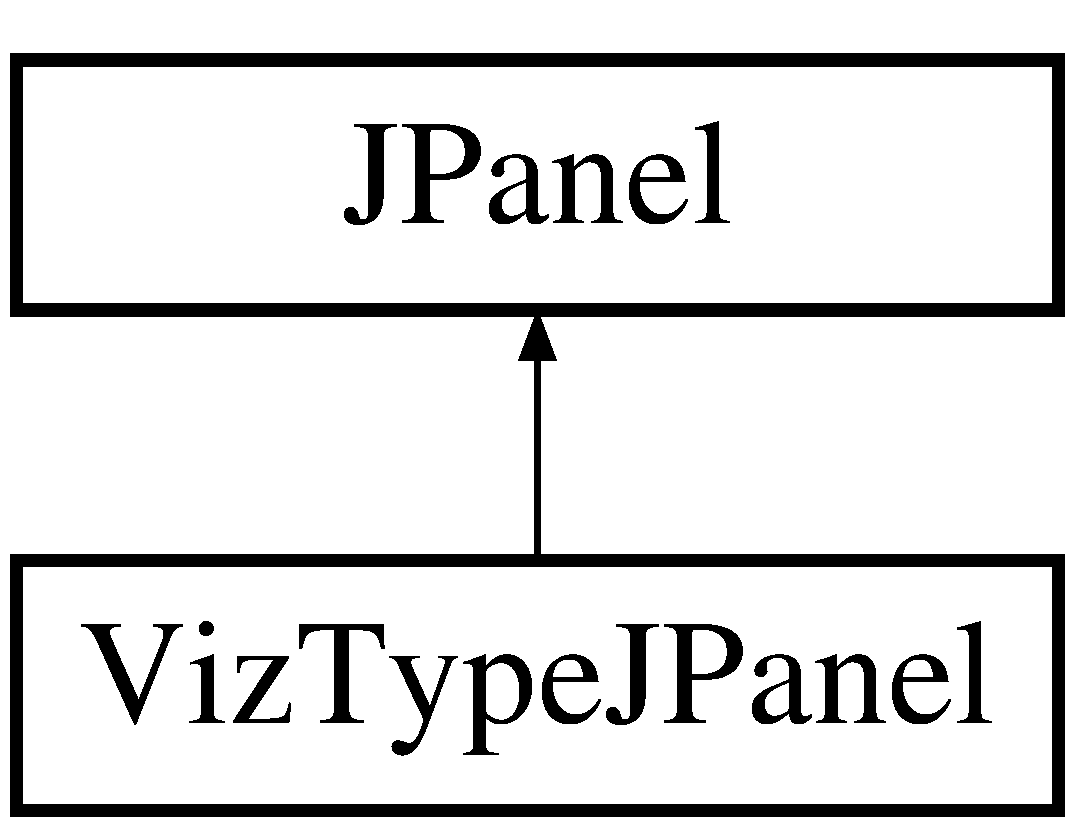
\includegraphics[height=2.000000cm]{class_viz_type_j_panel}
\end{center}
\end{figure}
\subsection*{Public Member Functions}
\begin{DoxyCompactItemize}
\item 
\hyperlink{class_viz_type_j_panel_ade1f7a00feed7a67bffabbaf9762f20f}{Viz\-Type\-J\-Panel} ()
\item 
\hyperlink{class_viz_type_j_panel_ab94442b4a1e1906ca3121fefcead19fa}{Viz\-Type\-J\-Panel} (boolean b)
\item 
J\-Toggle\-Button \hyperlink{class_viz_type_j_panel_a1d7f828f25ee2f352df65055e206178a}{Get\-Column\-Chart\-Button} ()
\item 
J\-Toggle\-Button \hyperlink{class_viz_type_j_panel_ae0e3195c99ed0025b23fb1dc72268b86}{Get\-Pie\-Chart\-Button} ()
\item 
J\-Toggle\-Button \hyperlink{class_viz_type_j_panel_a0550cb9b18806122a76a5dc600ad861a}{Get\-Line\-Chart\-Button} ()
\item 
J\-Toggle\-Button \hyperlink{class_viz_type_j_panel_a1d11994e9ddc79724ff8891280a71b32}{Get\-Bubble\-Chart\-Button} ()
\item 
J\-Toggle\-Button \hyperlink{class_viz_type_j_panel_aa16fca19c0ef36ff6cdf5b408ba2fbf1}{Get\-Scatter\-Chart\-Button} ()
\item 
J\-Toggle\-Button \hyperlink{class_viz_type_j_panel_aff060b4c6d74adbe43c674e007ff632a}{Get\-Area\-Chart\-Button} ()
\item 
J\-Toggle\-Button \hyperlink{class_viz_type_j_panel_a901113d4dd60480e8322182dc81de871}{Get\-Polar\-Chart\-Button} ()
\item 
J\-Toggle\-Button \hyperlink{class_viz_type_j_panel_a48853498dd3ae16b395b1a84044531d2}{Get\-Table\-View\-Button} ()
\item 
Boolean \hyperlink{class_viz_type_j_panel_a2dffefeb21c55d793593b1dacb364cf9}{Bubble\-Chart\-Button} ()
\item 
boolean \hyperlink{class_viz_type_j_panel_a83704bbce2513028139d3acea7a85907}{Set\-B\-V} (\hyperlink{class_bob_viz}{Bob\-Viz} bv)
\item 
int \hyperlink{class_viz_type_j_panel_adfd6c664764e55323f59ec7991be02d6}{Get\-Panel\-Width} ()
\item 
int \hyperlink{class_viz_type_j_panel_afabba3b86d50daf0627d3f5a1ced0681}{Get\-Panel\-Height} ()
\item 
void \hyperlink{class_viz_type_j_panel_a1e5bbe625fdca3098a662b73fa252fae}{Set\-Table\-View\-Button} (J\-Toggle\-Button m\-\_\-\-Table\-View\-Button)
\end{DoxyCompactItemize}
\subsection*{Static Public Member Functions}
\begin{DoxyCompactItemize}
\item 
static void \hyperlink{class_viz_type_j_panel_aac218445a0f5192f93b9e5d034d4cf71}{main} (String\mbox{[}$\,$\mbox{]} args)
\end{DoxyCompactItemize}


\subsection{Detailed Description}
This class provides the user with a list of different visualisation types to choose from. 

\begin{DoxyDate}{Date}
30/04/2013 
\end{DoxyDate}
\begin{DoxySeeAlso}{See Also}
\hyperlink{_dataset_8java}{Dataset.\-java} 
\end{DoxySeeAlso}


\subsection{Constructor \& Destructor Documentation}
\hypertarget{class_viz_type_j_panel_ade1f7a00feed7a67bffabbaf9762f20f}{\index{Viz\-Type\-J\-Panel@{Viz\-Type\-J\-Panel}!Viz\-Type\-J\-Panel@{Viz\-Type\-J\-Panel}}
\index{Viz\-Type\-J\-Panel@{Viz\-Type\-J\-Panel}!VizTypeJPanel@{Viz\-Type\-J\-Panel}}
\subsubsection[{Viz\-Type\-J\-Panel}]{\setlength{\rightskip}{0pt plus 5cm}Viz\-Type\-J\-Panel.\-Viz\-Type\-J\-Panel (
\begin{DoxyParamCaption}
{}
\end{DoxyParamCaption}
)}}\label{class_viz_type_j_panel_ade1f7a00feed7a67bffabbaf9762f20f}
Adding them to a button group will allow only a single button to be toggled at any time
\begin{DoxyCode}
36                            \{
37         \textcolor{comment}{/* set new dimension for VizTypeJPanel */}
38         Dimension size = getPreferredSize();
39         
40         \textcolor{comment}{/* set height and size for VizTypeJPanel */}
41         size.width = PAN\_WIDTH;
42         size.height = PAN\_HEIGHT;
43         setPreferredSize( size );
44         
45         setBorder( BorderFactory.createTitledBorder(
46                 BorderFactory.createLineBorder( Color.GRAY ), \textcolor{stringliteral}{"Select visualisation"}) );
47         
48         \textcolor{comment}{/* set new layout */}
49         setLayout( \textcolor{keyword}{new} FlowLayout( FlowLayout.CENTER ) );
50         
51         \textcolor{comment}{/* create new JPanel */}
52         JPanel centerJPan = \textcolor{keyword}{new} JPanel();
53         \textcolor{comment}{/* set new layout for centerJPan */}
54         centerJPan.setLayout( \textcolor{keyword}{new} GridLayout( GRID\_ROW, GRID\_COL, GRID\_VGAP, 
55                 GRID\_HGAP ) );
56        
61         ButtonGroup buttonGroup = \textcolor{keyword}{new} ButtonGroup();
62         buttonGroup.add(m\_ColumnChartButton);
63         buttonGroup.add(m\_PieChartButton);
64         buttonGroup.add(m\_LineChartButton);
65         buttonGroup.add(m\_BubbleChartButton);
66         buttonGroup.add(m\_ScatterPlotButton);
67         buttonGroup.add(m\_AreaChartButton);
68         buttonGroup.add(m\_PolarChartButton);
69         
70         centerJPan.add(m\_ColumnChartButton);
71         m\_ColumnChartButton.setSelected(\textcolor{keyword}{true});
72         centerJPan.add(m\_PieChartButton);
73         centerJPan.add(m\_LineChartButton);
74         centerJPan.add(m\_BubbleChartButton);
75         centerJPan.add(m\_ScatterPlotButton);
76         centerJPan.add(m\_AreaChartButton);
77         centerJPan.add(m\_PolarChartButton);
78         centerJPan.add(m\_TableViewButton);
79         
80          \textcolor{comment}{/* add centerJPan to VizTypeJPanel */}
81         add( centerJPan );
82         
83         \textcolor{comment}{/* set listeners */}
84         VizTypeJPanelEventHandler vTEventHandler = \textcolor{keyword}{new} 
85                 VizTypeJPanelEventHandler();
86         m\_BubbleChartButton.addItemListener(vTEventHandler);
87     \}
\end{DoxyCode}
\hypertarget{class_viz_type_j_panel_ab94442b4a1e1906ca3121fefcead19fa}{\index{Viz\-Type\-J\-Panel@{Viz\-Type\-J\-Panel}!Viz\-Type\-J\-Panel@{Viz\-Type\-J\-Panel}}
\index{Viz\-Type\-J\-Panel@{Viz\-Type\-J\-Panel}!VizTypeJPanel@{Viz\-Type\-J\-Panel}}
\subsubsection[{Viz\-Type\-J\-Panel}]{\setlength{\rightskip}{0pt plus 5cm}Viz\-Type\-J\-Panel.\-Viz\-Type\-J\-Panel (
\begin{DoxyParamCaption}
\item[{boolean}]{b}
\end{DoxyParamCaption}
)}}\label{class_viz_type_j_panel_ab94442b4a1e1906ca3121fefcead19fa}

\begin{DoxyCode}
89 \{\}
\end{DoxyCode}


\subsection{Member Function Documentation}
\hypertarget{class_viz_type_j_panel_a2dffefeb21c55d793593b1dacb364cf9}{\index{Viz\-Type\-J\-Panel@{Viz\-Type\-J\-Panel}!Bubble\-Chart\-Button@{Bubble\-Chart\-Button}}
\index{Bubble\-Chart\-Button@{Bubble\-Chart\-Button}!VizTypeJPanel@{Viz\-Type\-J\-Panel}}
\subsubsection[{Bubble\-Chart\-Button}]{\setlength{\rightskip}{0pt plus 5cm}Boolean Viz\-Type\-J\-Panel.\-Bubble\-Chart\-Button (
\begin{DoxyParamCaption}
{}
\end{DoxyParamCaption}
)}}\label{class_viz_type_j_panel_a2dffefeb21c55d793593b1dacb364cf9}

\begin{DoxyCode}
147                                       \{
148         \textcolor{keywordflow}{return} m\_BubbleChartButton.isSelected();
149     \}
\end{DoxyCode}
\hypertarget{class_viz_type_j_panel_aff060b4c6d74adbe43c674e007ff632a}{\index{Viz\-Type\-J\-Panel@{Viz\-Type\-J\-Panel}!Get\-Area\-Chart\-Button@{Get\-Area\-Chart\-Button}}
\index{Get\-Area\-Chart\-Button@{Get\-Area\-Chart\-Button}!VizTypeJPanel@{Viz\-Type\-J\-Panel}}
\subsubsection[{Get\-Area\-Chart\-Button}]{\setlength{\rightskip}{0pt plus 5cm}J\-Toggle\-Button Viz\-Type\-J\-Panel.\-Get\-Area\-Chart\-Button (
\begin{DoxyParamCaption}
{}
\end{DoxyParamCaption}
)}}\label{class_viz_type_j_panel_aff060b4c6d74adbe43c674e007ff632a}
Area \hyperlink{interface_chart}{Chart} Button \begin{DoxyReturn}{Returns}
Are \hyperlink{interface_chart}{Chart} m\-\_\-\-Area\-Chart\-Button 
\end{DoxyReturn}

\begin{DoxyCode}
130                                               \{
131         \textcolor{keywordflow}{return} m\_AreaChartButton;
132     \}
\end{DoxyCode}
\hypertarget{class_viz_type_j_panel_a1d11994e9ddc79724ff8891280a71b32}{\index{Viz\-Type\-J\-Panel@{Viz\-Type\-J\-Panel}!Get\-Bubble\-Chart\-Button@{Get\-Bubble\-Chart\-Button}}
\index{Get\-Bubble\-Chart\-Button@{Get\-Bubble\-Chart\-Button}!VizTypeJPanel@{Viz\-Type\-J\-Panel}}
\subsubsection[{Get\-Bubble\-Chart\-Button}]{\setlength{\rightskip}{0pt plus 5cm}J\-Toggle\-Button Viz\-Type\-J\-Panel.\-Get\-Bubble\-Chart\-Button (
\begin{DoxyParamCaption}
{}
\end{DoxyParamCaption}
)}}\label{class_viz_type_j_panel_a1d11994e9ddc79724ff8891280a71b32}
Bubble \hyperlink{interface_chart}{Chart} Button \begin{DoxyReturn}{Returns}
Bubble \hyperlink{interface_chart}{Chart} m\-\_\-\-Bubble\-Chart\-Button 
\end{DoxyReturn}

\begin{DoxyCode}
116                                                 \{
117         \textcolor{keywordflow}{return} m\_BubbleChartButton;
118     \}
\end{DoxyCode}
\hypertarget{class_viz_type_j_panel_a1d7f828f25ee2f352df65055e206178a}{\index{Viz\-Type\-J\-Panel@{Viz\-Type\-J\-Panel}!Get\-Column\-Chart\-Button@{Get\-Column\-Chart\-Button}}
\index{Get\-Column\-Chart\-Button@{Get\-Column\-Chart\-Button}!VizTypeJPanel@{Viz\-Type\-J\-Panel}}
\subsubsection[{Get\-Column\-Chart\-Button}]{\setlength{\rightskip}{0pt plus 5cm}J\-Toggle\-Button Viz\-Type\-J\-Panel.\-Get\-Column\-Chart\-Button (
\begin{DoxyParamCaption}
{}
\end{DoxyParamCaption}
)}}\label{class_viz_type_j_panel_a1d7f828f25ee2f352df65055e206178a}
Column \hyperlink{interface_chart}{Chart} Button \begin{DoxyReturn}{Returns}
Column \hyperlink{interface_chart}{Chart} m\-\_\-\-Column\-Chart\-Button 
\end{DoxyReturn}

\begin{DoxyCode}
95                                                 \{
96         \textcolor{keywordflow}{return} m\_ColumnChartButton;
97     \}
\end{DoxyCode}
\hypertarget{class_viz_type_j_panel_a0550cb9b18806122a76a5dc600ad861a}{\index{Viz\-Type\-J\-Panel@{Viz\-Type\-J\-Panel}!Get\-Line\-Chart\-Button@{Get\-Line\-Chart\-Button}}
\index{Get\-Line\-Chart\-Button@{Get\-Line\-Chart\-Button}!VizTypeJPanel@{Viz\-Type\-J\-Panel}}
\subsubsection[{Get\-Line\-Chart\-Button}]{\setlength{\rightskip}{0pt plus 5cm}J\-Toggle\-Button Viz\-Type\-J\-Panel.\-Get\-Line\-Chart\-Button (
\begin{DoxyParamCaption}
{}
\end{DoxyParamCaption}
)}}\label{class_viz_type_j_panel_a0550cb9b18806122a76a5dc600ad861a}
Line \hyperlink{interface_chart}{Chart} Button \begin{DoxyReturn}{Returns}
Line \hyperlink{interface_chart}{Chart} m\-\_\-\-Line\-Chart\-Button 
\end{DoxyReturn}

\begin{DoxyCode}
109                                               \{
110         \textcolor{keywordflow}{return} m\_LineChartButton;
111     \}
\end{DoxyCode}
\hypertarget{class_viz_type_j_panel_afabba3b86d50daf0627d3f5a1ced0681}{\index{Viz\-Type\-J\-Panel@{Viz\-Type\-J\-Panel}!Get\-Panel\-Height@{Get\-Panel\-Height}}
\index{Get\-Panel\-Height@{Get\-Panel\-Height}!VizTypeJPanel@{Viz\-Type\-J\-Panel}}
\subsubsection[{Get\-Panel\-Height}]{\setlength{\rightskip}{0pt plus 5cm}int Viz\-Type\-J\-Panel.\-Get\-Panel\-Height (
\begin{DoxyParamCaption}
{}
\end{DoxyParamCaption}
)}}\label{class_viz_type_j_panel_afabba3b86d50daf0627d3f5a1ced0681}
Gets Panel Height \begin{DoxyReturn}{Returns}
P\-A\-N\-\_\-\-Height 
\end{DoxyReturn}

\begin{DoxyCode}
194                                 \{
195         \textcolor{keywordflow}{return} PAN\_HEIGHT;
196     \}
\end{DoxyCode}
\hypertarget{class_viz_type_j_panel_adfd6c664764e55323f59ec7991be02d6}{\index{Viz\-Type\-J\-Panel@{Viz\-Type\-J\-Panel}!Get\-Panel\-Width@{Get\-Panel\-Width}}
\index{Get\-Panel\-Width@{Get\-Panel\-Width}!VizTypeJPanel@{Viz\-Type\-J\-Panel}}
\subsubsection[{Get\-Panel\-Width}]{\setlength{\rightskip}{0pt plus 5cm}int Viz\-Type\-J\-Panel.\-Get\-Panel\-Width (
\begin{DoxyParamCaption}
{}
\end{DoxyParamCaption}
)}}\label{class_viz_type_j_panel_adfd6c664764e55323f59ec7991be02d6}
Gets Panel Width \begin{DoxyReturn}{Returns}
P\-A\-N\-\_\-\-W\-I\-D\-T\-H 
\end{DoxyReturn}

\begin{DoxyCode}
187                                \{
188         \textcolor{keywordflow}{return} PAN\_WIDTH;
189     \}
\end{DoxyCode}
\hypertarget{class_viz_type_j_panel_ae0e3195c99ed0025b23fb1dc72268b86}{\index{Viz\-Type\-J\-Panel@{Viz\-Type\-J\-Panel}!Get\-Pie\-Chart\-Button@{Get\-Pie\-Chart\-Button}}
\index{Get\-Pie\-Chart\-Button@{Get\-Pie\-Chart\-Button}!VizTypeJPanel@{Viz\-Type\-J\-Panel}}
\subsubsection[{Get\-Pie\-Chart\-Button}]{\setlength{\rightskip}{0pt plus 5cm}J\-Toggle\-Button Viz\-Type\-J\-Panel.\-Get\-Pie\-Chart\-Button (
\begin{DoxyParamCaption}
{}
\end{DoxyParamCaption}
)}}\label{class_viz_type_j_panel_ae0e3195c99ed0025b23fb1dc72268b86}
Pie \hyperlink{interface_chart}{Chart} Button \begin{DoxyReturn}{Returns}
Pie \hyperlink{interface_chart}{Chart} m\-\_\-\-Pie\-Chart\-Button 
\end{DoxyReturn}

\begin{DoxyCode}
102                                              \{
103         \textcolor{keywordflow}{return} m\_PieChartButton;
104     \}
\end{DoxyCode}
\hypertarget{class_viz_type_j_panel_a901113d4dd60480e8322182dc81de871}{\index{Viz\-Type\-J\-Panel@{Viz\-Type\-J\-Panel}!Get\-Polar\-Chart\-Button@{Get\-Polar\-Chart\-Button}}
\index{Get\-Polar\-Chart\-Button@{Get\-Polar\-Chart\-Button}!VizTypeJPanel@{Viz\-Type\-J\-Panel}}
\subsubsection[{Get\-Polar\-Chart\-Button}]{\setlength{\rightskip}{0pt plus 5cm}J\-Toggle\-Button Viz\-Type\-J\-Panel.\-Get\-Polar\-Chart\-Button (
\begin{DoxyParamCaption}
{}
\end{DoxyParamCaption}
)}}\label{class_viz_type_j_panel_a901113d4dd60480e8322182dc81de871}
Polar \hyperlink{interface_chart}{Chart} Button \begin{DoxyReturn}{Returns}
Polar \hyperlink{interface_chart}{Chart} m\-\_\-\-Polar\-Chart\-Button 
\end{DoxyReturn}

\begin{DoxyCode}
137                                                \{
138         \textcolor{keywordflow}{return} m\_PolarChartButton;
139     \}
\end{DoxyCode}
\hypertarget{class_viz_type_j_panel_aa16fca19c0ef36ff6cdf5b408ba2fbf1}{\index{Viz\-Type\-J\-Panel@{Viz\-Type\-J\-Panel}!Get\-Scatter\-Chart\-Button@{Get\-Scatter\-Chart\-Button}}
\index{Get\-Scatter\-Chart\-Button@{Get\-Scatter\-Chart\-Button}!VizTypeJPanel@{Viz\-Type\-J\-Panel}}
\subsubsection[{Get\-Scatter\-Chart\-Button}]{\setlength{\rightskip}{0pt plus 5cm}J\-Toggle\-Button Viz\-Type\-J\-Panel.\-Get\-Scatter\-Chart\-Button (
\begin{DoxyParamCaption}
{}
\end{DoxyParamCaption}
)}}\label{class_viz_type_j_panel_aa16fca19c0ef36ff6cdf5b408ba2fbf1}
Scatter Plot Button \begin{DoxyReturn}{Returns}
Scatter Plot \hyperlink{interface_chart}{Chart} m\-\_\-\-Scatter\-Plot\-Button 
\end{DoxyReturn}

\begin{DoxyCode}
123                                                  \{
124         \textcolor{keywordflow}{return} m\_ScatterPlotButton;
125     \}
\end{DoxyCode}
\hypertarget{class_viz_type_j_panel_a48853498dd3ae16b395b1a84044531d2}{\index{Viz\-Type\-J\-Panel@{Viz\-Type\-J\-Panel}!Get\-Table\-View\-Button@{Get\-Table\-View\-Button}}
\index{Get\-Table\-View\-Button@{Get\-Table\-View\-Button}!VizTypeJPanel@{Viz\-Type\-J\-Panel}}
\subsubsection[{Get\-Table\-View\-Button}]{\setlength{\rightskip}{0pt plus 5cm}J\-Toggle\-Button Viz\-Type\-J\-Panel.\-Get\-Table\-View\-Button (
\begin{DoxyParamCaption}
{}
\end{DoxyParamCaption}
)}}\label{class_viz_type_j_panel_a48853498dd3ae16b395b1a84044531d2}
\hyperlink{class_table}{Table} View Button \begin{DoxyReturn}{Returns}
\hyperlink{class_table}{Table} View m\-\_\-\-Table\-View\-Button 
\end{DoxyReturn}

\begin{DoxyCode}
144                                               \{
145         \textcolor{keywordflow}{return} m\_TableViewButton;
146     \}
\end{DoxyCode}
\hypertarget{class_viz_type_j_panel_aac218445a0f5192f93b9e5d034d4cf71}{\index{Viz\-Type\-J\-Panel@{Viz\-Type\-J\-Panel}!main@{main}}
\index{main@{main}!VizTypeJPanel@{Viz\-Type\-J\-Panel}}
\subsubsection[{main}]{\setlength{\rightskip}{0pt plus 5cm}static void Viz\-Type\-J\-Panel.\-main (
\begin{DoxyParamCaption}
\item[{String\mbox{[}$\,$\mbox{]}}]{args}
\end{DoxyParamCaption}
)\hspace{0.3cm}{\ttfamily [static]}}}\label{class_viz_type_j_panel_aac218445a0f5192f93b9e5d034d4cf71}

\begin{DoxyCode}
198                                            \{
199         JFrame frame = \textcolor{keyword}{new} JFrame();
200         \hyperlink{class_viz_type_j_panel}{VizTypeJPanel} vTypeJPan = \textcolor{keyword}{new} \hyperlink{class_viz_type_j_panel_ade1f7a00feed7a67bffabbaf9762f20f}{VizTypeJPanel}();
201         JPanel panel = \textcolor{keyword}{new} JPanel();
202         panel.add(vTypeJPan);
203         frame.setSize(\textcolor{keyword}{new} Dimension(vTypeJPan.\hyperlink{class_viz_type_j_panel_afabba3b86d50daf0627d3f5a1ced0681}{GetPanelHeight}(),vTypeJPan.
      \hyperlink{class_viz_type_j_panel_adfd6c664764e55323f59ec7991be02d6}{GetPanelWidth}()));
204         frame.add(panel);
205         frame.pack();
206         frame.setVisible(\textcolor{keyword}{true});
207     \}
\end{DoxyCode}
\hypertarget{class_viz_type_j_panel_a83704bbce2513028139d3acea7a85907}{\index{Viz\-Type\-J\-Panel@{Viz\-Type\-J\-Panel}!Set\-B\-V@{Set\-B\-V}}
\index{Set\-B\-V@{Set\-B\-V}!VizTypeJPanel@{Viz\-Type\-J\-Panel}}
\subsubsection[{Set\-B\-V}]{\setlength{\rightskip}{0pt plus 5cm}boolean Viz\-Type\-J\-Panel.\-Set\-B\-V (
\begin{DoxyParamCaption}
\item[{{\bf Bob\-Viz}}]{bv}
\end{DoxyParamCaption}
)}}\label{class_viz_type_j_panel_a83704bbce2513028139d3acea7a85907}

\begin{DoxyParams}{Parameters}
{\em bv} & -\/ a \hyperlink{class_bob_viz}{Bob\-Viz} object \\
\hline
\end{DoxyParams}
\begin{DoxyReturn}{Returns}
T\-R\-U\-E on success 
\end{DoxyReturn}

\begin{DoxyCode}
170                                       \{
171         \textcolor{keywordtype}{boolean} test = \textcolor{keyword}{true};
172         \textcolor{keywordflow}{if}( ( test == \textcolor{keyword}{true} ) && ( bv == null ) ) \{
173             System.err.println( \textcolor{stringliteral}{"VizTypeJPanel::SetBV() ***Warning, object"}
174                     + \textcolor{stringliteral}{"is null. Value sent: "} + bv );
175         \} \textcolor{keywordflow}{else} \textcolor{keywordflow}{if} ( test == \textcolor{keyword}{true} ) \{
176             System.out.println( \textcolor{stringliteral}{"VizTypeJPanel::SetBV() Object is valid. Value"}
177                     + \textcolor{stringliteral}{"sent: "} + bv );
178         \}
179         m\_BV = bv;
180         \textcolor{keywordflow}{return} \textcolor{keyword}{true};
181     \}
\end{DoxyCode}
\hypertarget{class_viz_type_j_panel_a1e5bbe625fdca3098a662b73fa252fae}{\index{Viz\-Type\-J\-Panel@{Viz\-Type\-J\-Panel}!Set\-Table\-View\-Button@{Set\-Table\-View\-Button}}
\index{Set\-Table\-View\-Button@{Set\-Table\-View\-Button}!VizTypeJPanel@{Viz\-Type\-J\-Panel}}
\subsubsection[{Set\-Table\-View\-Button}]{\setlength{\rightskip}{0pt plus 5cm}void Viz\-Type\-J\-Panel.\-Set\-Table\-View\-Button (
\begin{DoxyParamCaption}
\item[{J\-Toggle\-Button}]{m\-\_\-\-Table\-View\-Button}
\end{DoxyParamCaption}
)}}\label{class_viz_type_j_panel_a1e5bbe625fdca3098a662b73fa252fae}

\begin{DoxyCode}
209                                                                     \{
210         this.m\_TableViewButton = m\_TableViewButton;
211     \}
\end{DoxyCode}


The documentation for this class was generated from the following file\-:\begin{DoxyCompactItemize}
\item 
\hyperlink{_viz_type_j_panel_8java}{Viz\-Type\-J\-Panel.\-java}\end{DoxyCompactItemize}

\chapter{File Documentation}
\hypertarget{_about_j_panel_8java}{\section{About\-J\-Panel.\-java File Reference}
\label{_about_j_panel_8java}\index{About\-J\-Panel.\-java@{About\-J\-Panel.\-java}}
}
\subsection*{Classes}
\begin{DoxyCompactItemize}
\item 
class \hyperlink{class_about_j_panel}{About\-J\-Panel}
\begin{DoxyCompactList}\small\item\em This class provides the user with information about the application. \end{DoxyCompactList}\end{DoxyCompactItemize}


\subsection{Detailed Description}
\begin{DoxyAuthor}{Author}
Rhys Owen A5, Bradley Coles-\/\-Perkins A6 
\end{DoxyAuthor}

\hypertarget{_area_chart_8java}{\section{Area\-Chart.\-java File Reference}
\label{_area_chart_8java}\index{Area\-Chart.\-java@{Area\-Chart.\-java}}
}
\subsection*{Classes}
\begin{DoxyCompactItemize}
\item 
class \hyperlink{class_area_chart}{Area\-Chart}
\begin{DoxyCompactList}\small\item\em A class that creates a single Area \hyperlink{interface_chart}{Chart} or two Area Charts visualizations from a 2\-D Array of data \textbackslash{} see \hyperlink{_graph_8java}{Graph.\-java}. \end{DoxyCompactList}\end{DoxyCompactItemize}


\subsection{Detailed Description}
\begin{DoxyAuthor}{Author}
Nathan Smith A5, Bradley Coles-\/\-Perkins A6 
\end{DoxyAuthor}

\hypertarget{_bob_viz_8java}{\section{Bob\-Viz.\-java File Reference}
\label{_bob_viz_8java}\index{Bob\-Viz.\-java@{Bob\-Viz.\-java}}
}
\subsection*{Classes}
\begin{DoxyCompactItemize}
\item 
class \hyperlink{class_bob_viz}{Bob\-Viz}
\begin{DoxyCompactList}\small\item\em This class provides the user with a simple G\-U\-I system. It initiates all instances used throughout the application. \end{DoxyCompactList}\end{DoxyCompactItemize}

\hypertarget{_bubble_chart_8java}{\section{Bubble\-Chart.\-java File Reference}
\label{_bubble_chart_8java}\index{Bubble\-Chart.\-java@{Bubble\-Chart.\-java}}
}
\subsection*{Classes}
\begin{DoxyCompactItemize}
\item 
class \hyperlink{class_bubble_chart}{Bubble\-Chart}
\begin{DoxyCompactList}\small\item\em A class that creates a single Bubble \hyperlink{interface_chart}{Chart} or two Bubble \hyperlink{interface_chart}{Chart} visualizations from a 2\-D Array of data \textbackslash{} see \hyperlink{_graph_8java}{Graph.\-java}. \end{DoxyCompactList}\end{DoxyCompactItemize}


\subsection{Detailed Description}
\begin{DoxyAuthor}{Author}
Nathan Smith A5, Bradley Coles-\/\-Perkins A6 
\end{DoxyAuthor}

\hypertarget{_chart_8java}{\section{Chart.\-java File Reference}
\label{_chart_8java}\index{Chart.\-java@{Chart.\-java}}
}
\subsection*{Classes}
\begin{DoxyCompactItemize}
\item 
class \hyperlink{interface_chart}{Chart}
\begin{DoxyCompactList}\small\item\em An interface for all chart classes. \end{DoxyCompactList}\end{DoxyCompactItemize}


\subsection{Detailed Description}
\begin{DoxyAuthor}{Author}
Phill Davies A5 
\end{DoxyAuthor}

\hypertarget{_colour_8java}{\section{Colour.\-java File Reference}
\label{_colour_8java}\index{Colour.\-java@{Colour.\-java}}
}
\subsection*{Classes}
\begin{DoxyCompactItemize}
\item 
class \hyperlink{class_colour}{Colour}
\begin{DoxyCompactList}\small\item\em This class provides user with a choice of some colours to be applied on objects from different graphs/charts/diagrams. \end{DoxyCompactList}\end{DoxyCompactItemize}

\hypertarget{_colour_map_8java}{\section{Colour\-Map.\-java File Reference}
\label{_colour_map_8java}\index{Colour\-Map.\-java@{Colour\-Map.\-java}}
}
\subsection*{Classes}
\begin{DoxyCompactItemize}
\item 
class \hyperlink{class_colour_map}{Colour\-Map}
\begin{DoxyCompactList}\small\item\em This class provides user with a choice of colours to be applied on objects from different graphs/charts/diagrams, and does all calculations needed in order to get it all working correctly. \end{DoxyCompactList}\end{DoxyCompactItemize}


\subsection{Detailed Description}
\begin{DoxyAuthor}{Author}
Herberts Markuns A5, Chrisopher Brennen A6 
\end{DoxyAuthor}

\hypertarget{_column_chart_8java}{\section{Column\-Chart.\-java File Reference}
\label{_column_chart_8java}\index{Column\-Chart.\-java@{Column\-Chart.\-java}}
}
\subsection*{Classes}
\begin{DoxyCompactItemize}
\item 
class \hyperlink{class_column_chart}{Column\-Chart}
\begin{DoxyCompactList}\small\item\em A class that displays specific data in a Column \hyperlink{interface_chart}{Chart} visualiser. \end{DoxyCompactList}\end{DoxyCompactItemize}


\subsection{Detailed Description}
\begin{DoxyAuthor}{Author}
Gavin Driscoll A4, Mark Leyshon A5, Bradley Coles-\/\-Perkins A6 
\end{DoxyAuthor}

\hypertarget{_data_attribute_8java}{\section{Data\-Attribute.\-java File Reference}
\label{_data_attribute_8java}\index{Data\-Attribute.\-java@{Data\-Attribute.\-java}}
}
\subsection*{Classes}
\begin{DoxyCompactItemize}
\item 
class \hyperlink{class_data_attribute}{Data\-Attribute}
\begin{DoxyCompactList}\small\item\em A class which is responsible setting graph attributes. \end{DoxyCompactList}\end{DoxyCompactItemize}

\hypertarget{_dataset_8java}{\section{Dataset.\-java File Reference}
\label{_dataset_8java}\index{Dataset.\-java@{Dataset.\-java}}
}
\subsection*{Classes}
\begin{DoxyCompactItemize}
\item 
class \hyperlink{class_dataset}{Dataset}
\begin{DoxyCompactList}\small\item\em A Class that Reads a data file format 'C\-S\-V' and Creates a 2\-D array and has methods to extract columns of data. \end{DoxyCompactList}\end{DoxyCompactItemize}

\hypertarget{_error_8java}{\section{Error.\-java File Reference}
\label{_error_8java}\index{Error.\-java@{Error.\-java}}
}
\subsection*{Classes}
\begin{DoxyCompactItemize}
\item 
class \hyperlink{class_error}{Error}
\begin{DoxyCompactList}\small\item\em A class designed to deal with errors and alerts the user. \end{DoxyCompactList}\end{DoxyCompactItemize}

\hypertarget{_graph_8java}{\section{Graph.\-java File Reference}
\label{_graph_8java}\index{Graph.\-java@{Graph.\-java}}
}
\subsection*{Classes}
\begin{DoxyCompactItemize}
\item 
class \hyperlink{interface_graph}{Graph}
\begin{DoxyCompactList}\small\item\em An interface for all graph classes. \end{DoxyCompactList}\end{DoxyCompactItemize}


\subsection{Detailed Description}
\begin{DoxyAuthor}{Author}
Phill Davies A4 
\end{DoxyAuthor}

\hypertarget{_group_p_d_m2application_8java}{\section{Group\-P\-D\-M2application.\-java File Reference}
\label{_group_p_d_m2application_8java}\index{Group\-P\-D\-M2application.\-java@{Group\-P\-D\-M2application.\-java}}
}
\subsection*{Classes}
\begin{DoxyCompactItemize}
\item 
class \hyperlink{class_group_p_d_m2application}{Group\-P\-D\-M2application}
\begin{DoxyCompactList}\small\item\em This class creates a new instance of \hyperlink{class_bob_viz}{Bob\-Viz} and parses it to all panels to ensure only one instance of \hyperlink{class_bob_viz}{Bob\-Viz} is ever used. \end{DoxyCompactList}\end{DoxyCompactItemize}

\hypertarget{_import_j_panel_8java}{\section{Import\-J\-Panel.\-java File Reference}
\label{_import_j_panel_8java}\index{Import\-J\-Panel.\-java@{Import\-J\-Panel.\-java}}
}
\subsection*{Classes}
\begin{DoxyCompactItemize}
\item 
class \hyperlink{class_import_j_panel}{Import\-J\-Panel}
\begin{DoxyCompactList}\small\item\em This class provides a import (C\-S\-V file) procedure. \end{DoxyCompactList}\end{DoxyCompactItemize}

\hypertarget{_information_j_panel_8java}{\section{Information\-J\-Panel.\-java File Reference}
\label{_information_j_panel_8java}\index{Information\-J\-Panel.\-java@{Information\-J\-Panel.\-java}}
}
\subsection*{Classes}
\begin{DoxyCompactItemize}
\item 
class \hyperlink{class_information_j_panel}{Information\-J\-Panel}
\begin{DoxyCompactList}\small\item\em A class designed to deal with the Information panel. \end{DoxyCompactList}\end{DoxyCompactItemize}

\hypertarget{_line_chart_8java}{\section{Line\-Chart.\-java File Reference}
\label{_line_chart_8java}\index{Line\-Chart.\-java@{Line\-Chart.\-java}}
}
\subsection*{Classes}
\begin{DoxyCompactItemize}
\item 
class \hyperlink{class_line_chart}{Line\-Chart}
\begin{DoxyCompactList}\small\item\em A class that creates a Line \hyperlink{interface_chart}{Chart} visualisation from a 2\-D Array of data. \end{DoxyCompactList}\end{DoxyCompactItemize}


\subsection{Detailed Description}
\begin{DoxyAuthor}{Author}
Bradley Coles-\/\-Perkins A5, A6 
\end{DoxyAuthor}

\hypertarget{_more_setting_j_panel_8java}{\section{More\-Setting\-J\-Panel.\-java File Reference}
\label{_more_setting_j_panel_8java}\index{More\-Setting\-J\-Panel.\-java@{More\-Setting\-J\-Panel.\-java}}
}
\subsection*{Classes}
\begin{DoxyCompactItemize}
\item 
class \hyperlink{class_more_setting_j_panel}{More\-Setting\-J\-Panel}
\begin{DoxyCompactList}\small\item\em A class designed to deal with the 'More Settings' panel. \end{DoxyCompactList}\end{DoxyCompactItemize}

\hypertarget{_pie_chart_8java}{\section{Pie\-Chart.\-java File Reference}
\label{_pie_chart_8java}\index{Pie\-Chart.\-java@{Pie\-Chart.\-java}}
}
\subsection*{Classes}
\begin{DoxyCompactItemize}
\item 
class \hyperlink{class_pie_chart}{Pie\-Chart}
\begin{DoxyCompactList}\small\item\em A simple class that displays data in a single Pie \hyperlink{interface_chart}{Chart}, or two Pie \hyperlink{interface_chart}{Chart} visualisations. \end{DoxyCompactList}\end{DoxyCompactItemize}


\subsection{Detailed Description}
\begin{DoxyAuthor}{Author}
Connor Mc\-Fadden A4, Leopold Stiegler A5, Bradley Coles-\/\-Perkins A6 
\end{DoxyAuthor}

\hypertarget{_polar_chart_8java}{\section{Polar\-Chart.\-java File Reference}
\label{_polar_chart_8java}\index{Polar\-Chart.\-java@{Polar\-Chart.\-java}}
}
\subsection*{Classes}
\begin{DoxyCompactItemize}
\item 
class \hyperlink{class_polar_chart}{Polar\-Chart}
\begin{DoxyCompactList}\small\item\em A class that creates a single Polar \hyperlink{interface_chart}{Chart} or two Polar \hyperlink{interface_chart}{Chart} visualisations from 2\-D Arrays of data \textbackslash{} see \hyperlink{_graph_8java}{Graph.\-java}. \end{DoxyCompactList}\end{DoxyCompactItemize}


\subsection{Detailed Description}
\begin{DoxyAuthor}{Author}
Mark Leyshon A5, Bradley Coles-\/\-Perkins A6 
\end{DoxyAuthor}

\hypertarget{_scatter_plot_graph_8java}{\section{Scatter\-Plot\-Graph.\-java File Reference}
\label{_scatter_plot_graph_8java}\index{Scatter\-Plot\-Graph.\-java@{Scatter\-Plot\-Graph.\-java}}
}
\subsection*{Classes}
\begin{DoxyCompactItemize}
\item 
class \hyperlink{class_scatter_plot_graph}{Scatter\-Plot\-Graph}
\begin{DoxyCompactList}\small\item\em A class that creates a single Scatter Plot \hyperlink{interface_graph}{Graph} or two Scatter Plot \hyperlink{interface_graph}{Graph} visualisations from a 2\-D Array of data. \end{DoxyCompactList}\end{DoxyCompactItemize}


\subsection{Detailed Description}
\begin{DoxyAuthor}{Author}
Phill Davies A4, Leopold Stiegler A5, Bradley Coles-\/\-Perkins A6 
\end{DoxyAuthor}

\hypertarget{_selection_viz_j_panel_8java}{\section{Selection\-Viz\-J\-Panel.\-java File Reference}
\label{_selection_viz_j_panel_8java}\index{Selection\-Viz\-J\-Panel.\-java@{Selection\-Viz\-J\-Panel.\-java}}
}
\subsection*{Classes}
\begin{DoxyCompactItemize}
\item 
class \hyperlink{class_selection_viz_j_panel}{Selection\-Viz\-J\-Panel}
\begin{DoxyCompactList}\small\item\em This class passes the data from the G\-U\-I to the constructors of the visualisation types. \end{DoxyCompactList}\end{DoxyCompactItemize}


\subsection{Detailed Description}
\begin{DoxyAuthor}{Author}
Rhys Owen A4, Bradley Coles-\/\-Perkins A5,A6 
\end{DoxyAuthor}

\hypertarget{_setting_j_panel_8java}{\section{Setting\-J\-Panel.\-java File Reference}
\label{_setting_j_panel_8java}\index{Setting\-J\-Panel.\-java@{Setting\-J\-Panel.\-java}}
}
\subsection*{Classes}
\begin{DoxyCompactItemize}
\item 
class \hyperlink{class_setting_j_panel}{Setting\-J\-Panel}
\begin{DoxyCompactList}\small\item\em This class provides the settings for each visualisation. \end{DoxyCompactList}\end{DoxyCompactItemize}

\hypertarget{_slideshow_8java}{\section{Slideshow.\-java File Reference}
\label{_slideshow_8java}\index{Slideshow.\-java@{Slideshow.\-java}}
}
\subsection*{Classes}
\begin{DoxyCompactItemize}
\item 
class \hyperlink{class_slideshow}{Slideshow}
\begin{DoxyCompactList}\small\item\em A class that creates a slideshow of a single \hyperlink{interface_chart}{Chart} or two \hyperlink{interface_chart}{Chart} visualizations \textbackslash{} see \hyperlink{_graph_8java}{Graph.\-java}. \end{DoxyCompactList}\end{DoxyCompactItemize}


\subsection{Detailed Description}
\begin{DoxyAuthor}{Author}
Bradley Coles-\/\-Perkins A6 
\end{DoxyAuthor}

\hypertarget{_status_j_panel_8java}{\section{Status\-J\-Panel.\-java File Reference}
\label{_status_j_panel_8java}\index{Status\-J\-Panel.\-java@{Status\-J\-Panel.\-java}}
}
\subsection*{Classes}
\begin{DoxyCompactItemize}
\item 
class \hyperlink{class_status_j_panel}{Status\-J\-Panel}
\begin{DoxyCompactList}\small\item\em This class will display the status of the application. \end{DoxyCompactList}\end{DoxyCompactItemize}

\hypertarget{_table_8java}{\section{Table.\-java File Reference}
\label{_table_8java}\index{Table.\-java@{Table.\-java}}
}
\subsection*{Classes}
\begin{DoxyCompactItemize}
\item 
class \hyperlink{class_table}{Table}
\begin{DoxyCompactList}\small\item\em A simple class that displays data in a table visualisation. \end{DoxyCompactList}\end{DoxyCompactItemize}


\subsection{Detailed Description}
\begin{DoxyAuthor}{Author}
Connor Mc\-Fadden A4, Bradley Coles-\/\-Perkins A6 
\end{DoxyAuthor}

\hypertarget{_time_stamp_8java}{\section{Time\-Stamp.\-java File Reference}
\label{_time_stamp_8java}\index{Time\-Stamp.\-java@{Time\-Stamp.\-java}}
}
\subsection*{Classes}
\begin{DoxyCompactItemize}
\item 
class {\bfseries Time\-Stamp}
\begin{DoxyCompactList}\small\item\em Class to generate a time stamp. \end{DoxyCompactList}\end{DoxyCompactItemize}


\subsection{Detailed Description}
\begin{DoxyAuthor}{Author}
Arran Willis A5 
\end{DoxyAuthor}

\hypertarget{_visualisation_8java}{\section{Visualisation.\-java File Reference}
\label{_visualisation_8java}\index{Visualisation.\-java@{Visualisation.\-java}}
}
\subsection*{Classes}
\begin{DoxyCompactItemize}
\item 
class \hyperlink{class_visualisation}{Visualisation}
\begin{DoxyCompactList}\small\item\em A class that displays specific data in a Column \hyperlink{interface_chart}{Chart} visualiser. \end{DoxyCompactList}\end{DoxyCompactItemize}

\hypertarget{_viz_type_j_panel_8java}{\section{Viz\-Type\-J\-Panel.\-java File Reference}
\label{_viz_type_j_panel_8java}\index{Viz\-Type\-J\-Panel.\-java@{Viz\-Type\-J\-Panel.\-java}}
}
\subsection*{Classes}
\begin{DoxyCompactItemize}
\item 
class \hyperlink{class_viz_type_j_panel}{Viz\-Type\-J\-Panel}
\begin{DoxyCompactList}\small\item\em This class provides the user with a list of different visualisation types to choose from. \end{DoxyCompactList}\end{DoxyCompactItemize}


\subsection{Detailed Description}
\begin{DoxyAuthor}{Author}
Rhys Owen A4, Leopold Stiegler A5, Bradley Coles-\/\-Perkins A6 
\end{DoxyAuthor}

\addcontentsline{toc}{part}{Index}
\printindex
\end{document}
